% Judul dokumen
\title{Buku Tugas Akhir ITS}
\author{Uzlahwasata, Dzakirozaan}

% Pengaturan ukuran teks dan bentuk halaman dua sisi
\documentclass[12pt,twoside]{report}

% Pengaturan ukuran halaman dan margin
\usepackage[a4paper,top=30mm,left=30mm,right=20mm,bottom=25mm]{geometry}

% Pengaturan ukuran spasi
\usepackage[singlespacing]{setspace}

% Pengaturan detail pada file PDF
\usepackage[pdfauthor={\@author},bookmarksnumbered,pdfborder={0 0 0}]{hyperref}

% Pengaturan jenis karakter
\usepackage[utf8]{inputenc}

% Pengaturan pewarnaan
\usepackage[table,xcdraw]{xcolor}

% Pengaturan kutipan artikel
\usepackage[style=apa, backend=biber]{biblatex}

% Package lainnya
\usepackage{changepage}
\usepackage{enumitem}
\usepackage{eso-pic}
\usepackage{txfonts} % Font times
\usepackage{etoolbox}
\usepackage{graphicx}
\usepackage{lipsum}
\usepackage{longtable}
\usepackage{tabularx}
\usepackage{wrapfig}
\usepackage{float}

% Package tambahan
\usepackage{multirow}
\usepackage{multicol}
\usepackage{amsmath}
\usepackage{adjustbox}
\usepackage{booktabs}
\usepackage{tabularray}

% Definisi untuk "Hati ini sengaja dikosongkan"
\patchcmd{\cleardoublepage}{\hbox{}}{
  \thispagestyle{empty}
  \vspace*{\fill}
  \begin{center}\textit{[Halaman ini sengaja dikosongkan]}\end{center}
  \vfill}{}{}

% Pengaturan penomoran halaman
\usepackage{fancyhdr}
\fancyhf{}
\renewcommand{\headrulewidth}{0pt}
\pagestyle{fancy}
\fancyfoot[LE,RO]{\thepage}
\patchcmd{\chapter}{plain}{fancy}{}{}
\patchcmd{\chapter}{empty}{plain}{}{}

% Command untuk bulan
\newcommand{\MONTH}{%
  \ifcase\the\month
  \or Januari% 1
  \or Februari% 2
  \or Maret% 3
  \or April% 4
  \or Mei% 5
  \or Juni% 6
  \or Juli% 7
  \or Agustus% 8
  \or September% 9
  \or Oktober% 10
  \or November% 11
  \or Desember% 12
  \fi}
\newcommand{\ENGMONTH}{%
  \ifcase\the\month
  \or January% 1
  \or February% 2
  \or March% 3
  \or April% 4
  \or May% 5
  \or June% 6
  \or July% 7
  \or August% 8
  \or September% 9
  \or October% 10
  \or November% 11
  \or December% 12
  \fi}

% Pengaturan format judul bab
\usepackage{titlesec}
\titleformat{\chapter}[display]{\bfseries\Large}{BAB \centering\Roman{chapter}}{0ex}{\vspace{0ex}\centering}
\titleformat{\section}{\bfseries\large}{\MakeUppercase{\thesection}}{1ex}{\vspace{1ex}}
\titleformat{\subsection}{\bfseries\large}{\MakeUppercase{\thesubsection}}{1ex}{}
\titleformat{\subsubsection}{\bfseries\large}{\MakeUppercase{\thesubsubsection}}{1ex}{}
\titlespacing{\chapter}{0ex}{0ex}{4ex}
\titlespacing{\section}{0ex}{1ex}{0ex}
\titlespacing{\subsection}{0ex}{0.5ex}{0ex}
\titlespacing{\subsubsection}{0ex}{0.5ex}{0ex}

% Atur variabel berikut sesuai namanya

% nama
\newcommand{\name}{Dzakirozaan Uzlahwasata}
\newcommand{\authorname}{Uzlahwasata, Dzakirozaan}
\newcommand{\nickname}{Dzakirozaan}
\newcommand{\advisor}{Annisaa Sri Indrawanti, S. Kom., M. Kom.}
\newcommand{\coadvisor}{Fuad Dary Rosyadi, S.Kom., M.Kom.}
\newcommand{\examinerone}{Dr. Galileo Galilei, S.T., M.Sc}
\newcommand{\examinertwo}{Friedrich Nietzsche, S.T., M.Sc}
\newcommand{\headofdepartment}{Dr.tech.Ir. Raden Venantius Hari Ginardi, M.Sc}

% identitas
\newcommand{\nrp}{5027211066}
\newcommand{\advisornip}{19910523 202012 2 018}
\newcommand{\coadvisornip}{19960910 202406 1 003}
\newcommand{\examineronenip}{18560710 194301 1 001}
\newcommand{\examinertwonip}{18560710 194301 1 001}
\newcommand{\examinerthreenip}{18560710 194301 1 001}
\newcommand{\headofdepartmentnip}{19650518 199203 1 003}

% judul
\newcommand{\tatitle}{OPTIMASI \textit{TASK SCHEDULING} MENGGUNAKAN \textit{ARTIFICAL BEE COLONY} (ABC) DAN \textit{ELITE OPPOSITION-BASED LEARNING} (EOBL) PADA \textit{CLOUD ENVIRONMENT}}
\newcommand{\engtatitle}{\emph{TASK SCHEDULING OPTIMIZATION USING ARTIFICIAL BEE COLONY (ABC) AND ELITE OPPOSITION-BASED LEARNING (EOBL) IN CLOUD ENVIRONMENT}}

% tempat
\newcommand{\place}{Surabaya}

% jurusan
\newcommand{\studyprogram}{Teknologi Informasi}
\newcommand{\engstudyprogram}{Information Technology}

% fakultas
\newcommand{\faculty}{Teknologi Elektro dan Informatika Cerdas}
\newcommand{\engfaculty}{Intelligent Electrical and Informatics Technology}

% singkatan fakultas
\newcommand{\facultyshort}{FTEIC}
\newcommand{\engfacultyshort}{ELECTICS}

% departemen
\newcommand{\department}{Teknologi Informasi}
\newcommand{\engdepartment}{Information Technology}

% kode mata kuliah
\newcommand{\coursecode}{ET234801}


% Tambahkan format tanda hubung yang benar di sini
\hyphenation{
  me-nga-dop-si
  pro-ses
  sched-ul-ing
  me-to-do-lo-gi
  di-kum-pul-kan
  ber-da-sar-kan
  ri-ngan
  me-la-ku-kan
  me-nye-le-sai-kan
  meng-in-is-i-al-i-sa-si
  ef-i-si-en-si
  clo-ud-let
  me-ngum-pul-kan
  meng-in-di-ka-si-kan
  meng-gam-bar-kan
  im-ple-men-ta-si-nya
  ma-ke-span-sta-rt
  me-la-lu-i
  me-nga-lo-ka-si-kan
  fu-ng-si
  ting-kat
  de-fa-ult
  me-to-de
  thr-ough-put
  me-mer-lu-kan
  se-per-ti
  me-na-nga-ni
  st-art
  me-th-od
  da-ta-set
  me-ning-kat-kan
  co-lo-ny
  pe-nu-lis
  ak-hir
}

% Menambahkan resource daftar pustaka
\addbibresource{pustaka/pustaka.bib}

% Pengaturan format potongan kode
\usepackage{listings}
\definecolor{comment}{RGB}{0,128,0}
\definecolor{string}{RGB}{255,0,0}
\definecolor{keyword}{RGB}{0,0,255}
\lstdefinestyle{codestyle}{
  commentstyle=\color{comment},
  stringstyle=\color{string},
  keywordstyle=\color{keyword},
  basicstyle=\footnotesize\ttfamily,
  numbers=left,
  numberstyle=\tiny,
  numbersep=5pt,
  frame=lines,
  breaklines=true,
  prebreak=\raisebox{0ex}[0ex][0ex]{\ensuremath{\hookleftarrow}},
  showstringspaces=false,
  upquote=true,
  tabsize=2,
}
\lstset{style=codestyle, captionpos=b}
\renewcommand{\lstlistingname}{Kode Sumber}

% Isi keseluruhan dokumen
\begin{document}

% Sampul luar Bahasa Indonesia
\newcommand\covercontents{sampul/konten-id.tex}
\AddToShipoutPictureBG*{
  \AtPageLowerLeft{
    % Ubah nilai berikut jika posisi horizontal background tidak sesuai
    \hspace{-3.25mm}

    % Ubah nilai berikut jika posisi vertikal background tidak sesuai
    \raisebox{0mm}{
      
\includegraphics[width=\paperwidth,height=\paperheight]{sampul/gambar/sampul-luar.png}
    }
  }
}

% Menyembunyikan nomor halaman
\thispagestyle{empty}

% Pengaturan margin untuk menyesuaikan konten sampul
\newgeometry{
  top=55mm,
  left=30mm,
  right=20mm,
  bottom=20mm
}

\begin{flushleft}

  % Pemilihan font sans serif
  \sffamily

  % Pemilihan warna font putih
  \color{white}

  % Pemilihan font bold
  \fontseries{bx}
  \selectfont
  \begin{spacing}{1.5}
    \input{\covercontents}
  \end{spacing}

\end{flushleft}

\restoregeometry


% Atur ulang penomoran halaman
\setcounter{page}{1}

% Sampul dalam Bahasa Indonesia
\renewcommand\covercontents{sampul/konten-id.tex}
\AddToShipoutPictureBG*{
  \AtPageLowerLeft{
    % Ubah nilai berikut jika posisi horizontal background tidak sesuai
    \hspace{-4mm}

    % Ubah nilai berikut jika posisi vertikal background tidak sesuai
    \raisebox{0mm}{
      
\includegraphics[width=\paperwidth,height=\paperheight]{sampul/gambar/sampul-luar-tipis.png}
    }
  }
}

% Menyembunyikan nomor halaman
\thispagestyle{empty}

% Pengaturan margin untuk menyesuaikan konten sampul
\newgeometry{
  top=65mm,
  left=30mm,
  right=30mm,
  bottom=20mm
}

\begin{flushleft}

  % Pemilihan font sans serif
  \sffamily

  % Pemilihan font bold
  \fontseries{bx}
  \selectfont
  \begin{spacing}{1.5}
    \input{\covercontents}
  \end{spacing}

\end{flushleft}

\restoregeometry

\clearpage
\cleardoublepage

% Sampul dalam Bahasa Inggris
\renewcommand\covercontents{sampul/konten-en.tex}
\AddToShipoutPictureBG*{
  \AtPageLowerLeft{
    % Ubah nilai berikut jika posisi horizontal background tidak sesuai
    \hspace{-4mm}

    % Ubah nilai berikut jika posisi vertikal background tidak sesuai
    \raisebox{0mm}{
      
\includegraphics[width=\paperwidth,height=\paperheight]{sampul/gambar/sampul-luar-tipis.png}
    }
  }
}

% Menyembunyikan nomor halaman
\thispagestyle{empty}

% Pengaturan margin untuk menyesuaikan konten sampul
\newgeometry{
  top=65mm,
  left=30mm,
  right=30mm,
  bottom=20mm
}

\begin{flushleft}

  % Pemilihan font sans serif
  \sffamily

  % Pemilihan font bold
  \fontseries{bx}
  \selectfont
  \begin{spacing}{1.5}
    \input{\covercontents}
  \end{spacing}

\end{flushleft}

\restoregeometry

\cleardoublepage

% Label tabel dan gambar dalam bahasa indonesia
\renewcommand{\figurename}{Gambar}
\renewcommand{\tablename}{Tabel}

% Pengaturan ukuran indentasi paragraf
\setlength{\parindent}{2em}

% Pengaturan ukuran spasi paragraf
\setlength{\parskip}{1ex}

% Lembar pengesahan
\begin{center}
  \large
  \textbf{LEMBAR PENGESAHAN}
\end{center}

% Menyembunyikan nomor halaman
\thispagestyle{empty}

\begin{center}
  \textbf{\tatitle{}}
\end{center}

\begingroup
% Pemilihan font ukuran small
\small

\begin{center}
  \textbf{TUGAS AKHIR}
  \\Diajukan untuk memenuhi salah satu syarat \\
  memperoleh gelar Sarjana Teknik pada \\
  Program Studi S-1 \studyprogram{} \\
  Departemen \department{} \\
  Fakultas \faculty{} \\
  Institut Teknologi Sepuluh Nopember
\end{center}

\begin{center}
  Oleh: \textbf{\name{}}
  \\NRP. \nrp{}
\end{center}

\begin{center}
  Disetujui oleh Tim Penguji Tugas Akhir:
\end{center}

\begingroup
% Menghilangkan padding
\setlength{\tabcolsep}{0pt}

\noindent
\begin{tabularx}{\textwidth}{X l}
  \advisor{}               & (Pembimbing I)                      \\
  NIP: \advisornip{}       &                                     \\
                           & ................................... \\
                           &                                     \\
                           &                                     \\
  \coadvisor{}             & (Pembimbing II)                     \\
  NIP: \coadvisornip{}     &                                     \\
                           & ................................... \\
                           &                                     \\
                           &                                     \\
  \examinerone{}.          & (Penguji I)                         \\
  NIP: \examineronenip{}   &                                     \\
                           & ................................... \\
                           &                                     \\
                           &                                     \\
  \examinertwo{}.          & (Penguji II)                        \\
  NIP: \examinertwonip{}   &                                     \\
                           & ................................... \\
                           &                                     \\
\end{tabularx}
\endgroup

\begin{center}
  Mengetahui, \\
  Kepala Departemen \department{} \facultyshort{} - ITS\\

  \vspace{8ex}

  \underline{\headofdepartment{}.} \\
  NIP. \headofdepartmentnip{}
\end{center}

\begin{center}
  \textbf{\MakeUppercase{\place{}}\\\MONTH{}, \the\year{}}
\end{center}
\endgroup

\cleardoublepage
\begin{center}
  \large
  \textbf{APPROVAL SHEET}
\end{center}

% Menyembunyikan nomor halaman
\thispagestyle{empty}

\begin{center}
  \textbf{\engtatitle{}}
\end{center}

\begingroup
% Pemilihan font ukuran small
\small

\begin{center}
  \textbf{FINAL PROJECT}
  \\Submitted to fulfill one of the requirements \\
  for obtaining a degree Bachelor of Engineering at \\
  Undergraduate Study Program of \engstudyprogram{} \\
  Department of \engdepartment{} \\
  Faculty of \engfaculty{} \\
  Sepuluh Nopember Institute of Technology
\end{center}

\begin{center}
  By: \textbf{\name{}}
  \\NRP. \nrp{}
\end{center}

\begin{center}
  Approved by Final Project Examiner Team:
\end{center}

\begingroup
% Menghilangkan padding
\setlength{\tabcolsep}{0pt}

\noindent
\begin{tabularx}{\textwidth}{X l}
  \advisor{}               & (Advisor I)                         \\
  NIP: \advisornip{}       &                                     \\
                           & ................................... \\
                           &                                     \\
                           &                                     \\
  \coadvisor{}             & (Co-Advisor II)                     \\
  NIP: \coadvisornip{}     &                                     \\
                           & ................................... \\
                           &                                     \\
                           &                                     \\
  \examinerone{}.          & (Examiner I)                        \\
  NIP: \examineronenip{}   &                                     \\
                           & ................................... \\
                           &                                     \\
                           &                                     \\
  \examinertwo{}.          & (Examiner II)                       \\
  NIP: \examinertwonip{}   &                                     \\
                           & ................................... \\
                           &                                     \\
\end{tabularx}
\endgroup


\begin{center}
  Acknowledged, \\
  Head of \engdepartment{} Department \engfacultyshort{} - ITS \\

  \vspace{8ex}

  \underline{\headofdepartment{}.} \\
  NIP. \headofdepartmentnip{}
\end{center}

\begin{center}
  \textbf{\MakeUppercase{\place{}}\\\ENGMONTH{}, \the\year{}}
\end{center}
\endgroup

\cleardoublepage

% Pernyataan keaslian
\begin{center}
  \large
  \textbf{PERNYATAAN ORISINALITAS}
\end{center}

% Menyembunyikan nomor halaman
\thispagestyle{empty}

\vspace{2ex}

% Ubah paragraf-paragraf berikut sesuai dengan yang ingin diisi pada pernyataan keaslian

\noindent Yang bertanda tangan dibawah ini:

\noindent\begin{tabularx}{\textwidth}{l l X}
                         &   &                            \\
  Nama Mahasiswa / NRP   & : & \name{} / \nrp{}           \\
  Departemen             & : & \department{}              \\
  Dosen Pembimbing / NIP & : & \advisor{} / \advisornip{} \\
                         &   &                            \\
\end{tabularx}

Dengan ini menyatakan bahwa Tugas Akhir dengan judul "\tatitle{}" adalah hasil karya sendiri, berfsifat orisinal, dan ditulis dengan mengikuti kaidah penulisan ilmiah.

Bilamana di kemudian hari ditemukan ketidaksesuaian dengan pernyataan ini, maka saya bersedia menerima sanksi sesuai dengan ketentuan yang berlaku di Institut Teknologi Sepuluh Nopember.

\vspace{8ex}

\noindent\begin{tabularx}{\textwidth}{X l}
                     & \place{}, \MONTH{} \the\year{} \\
                     &                                   \\
  Mengetahui         &                                   \\
  Dosen Pembimbing   & Mahasiswa                         \\
                     &                                   \\
                     &                                   \\
                     &                                   \\
                     &                                   \\
                     &                                   \\
  \advisor{}         & \name{}                           \\
  NIP. \advisornip{} & NRP. \nrp{}                       \\
\end{tabularx}

\cleardoublepage
\begin{center}
  \large
  \textbf{STATEMENT OF ORIGINALITY}
\end{center}

% Menyembunyikan nomor halaman
\thispagestyle{empty}

\vspace{2ex}

% Ubah paragraf-paragraf berikut sesuai dengan yang ingin diisi pada pernyataan keaslian

\noindent The undersigned below:

\noindent\begin{tabularx}{\textwidth}{l l X}
                        &   &                            \\
  Name of student / NRP & : & \name{} / \nrp{}           \\
  Department            & : & \engdepartment{}           \\
  Advisor / NIP         & : & \advisor{} / \advisornip{} \\
                        &   &                            \\
\end{tabularx}

Hereby declared that the Final Project with the title of "\engtatitle{}" is the result of my own work, is original, and is written by following the rules of scientific writing.

If in future there is a discrepancy with this statement, then I am willing to accept sanctions in accordance with provisions that apply at Sepuluh Nopember Institute of Technology.

\vspace{8ex}

\noindent\begin{tabularx}{\textwidth}{X l}
                     & \place{}, \ENGMONTH{} \the\year{} \\
                     &                                   \\
  Acknowledged       &                                   \\
  Advisor            & Student                           \\
                     &                                   \\
                     &                                   \\
                     &                                   \\
                     &                                   \\
                     &                                   \\
  \advisor{}         & \name{}                           \\
  NIP. \advisornip{} & NRP. \nrp{}                       \\
\end{tabularx}
\cleardoublepage

% Nomor halaman pembuka dimulai dari sini
\pagenumbering{roman}

% Abstrak Bahasa Indonesia
\begin{center}
  \large\textbf{ABSTRAK}
\end{center}

\addcontentsline{toc}{chapter}{ABSTRAK}

\vspace{2ex}

\begingroup
% Menghilangkan padding
\setlength{\tabcolsep}{0pt}

\noindent
\begin{tabularx}{\textwidth}{l >{\centering}m{2em} X}
  Nama Mahasiswa    & : & \name{}         \\

  Judul Tugas Akhir & : & \tatitle{}      \\

  Pembimbing        & : & 1. \advisor{}   \\
                    &   & 2. \coadvisor{} \\
\end{tabularx}
\endgroup

% Ubah paragraf berikut dengan abstrak dari tugas akhir
Penjadwalan tugas (\textit{task scheduling}) yang efisien pada lingkungan \textit{cloud computing} merupakan tantangan krusial untuk memaksimalkan penggunaan sumber daya. Algoritma \textit{Artificial Bee Colony} (ABC) yang umum digunakan sering kali mengalami kelemahan dalam hal pemanfaatan sumber daya dan cenderung terjebak pada solusi lokal. Untuk mengatasi masalah ini, penelitian ini mengusulkan optimasi melalui kombinasi algoritma ABC dengan pendekatan \textit{Elite Opposition-Based Learning} (EOBL). Metode ini diimplementasikan dengan strategi oposisi berdasarkan solusi elite guna memperluas ruang pencarian dan menghindari konvergensi prematur. Hasil pengujian menunjukkan bahwa pendekatan ABC-EOBL secara signifikan meningkatkan keseimbangan alokasi sumber daya, terbukti dari performa parameter \textit{imbalance degree} yang 18,40\% lebih efisien dibandingkan algoritma pembanding. Meskipun unggul dalam parameter \textit{imbalance degree}, penerapan EOBL menyebabkan penurunan kinerja pada metrik lain seperti \textit{makespan}, \textit{average start time}, \textit{average finish time}, \textit{average execution time}, \textit{average waiting time}, \textit{scheduling length}, \textit{throughput}, \textit{resource utilization}, dan \textit{energy consumption}, akibat meningkatnya kompleksitas pencarian. Kesimpulannya, metode ABC-EOBL menawarkan keuntungan signifikan untuk distribusi sumber daya yang seimbang, namun penggunaannya harus mempertimbangkan adanya \textit{trade-off} dengan efisiensi waktu eksekusi.

% Ubah kata-kata berikut dengan kata kunci dari tugas akhir
Kata Kunci: Penjadwalan Tugas, Komputasi Awan, \textit{Artificial Bee Colony}, \textit{Elite Opposition-Based Learning}.
\cleardoublepage

% Abstrak Bahasa Inggris
\begin{center}
  \large\textbf{ABSTRACT}
\end{center}

\addcontentsline{toc}{chapter}{ABSTRACT}

\vspace{2ex}

\begingroup
% Menghilangkan padding
\setlength{\tabcolsep}{0pt}

\noindent
\begin{tabularx}{\textwidth}{l >{\centering}m{3em} X}
  \emph{Name}     & : & \name{}         \\

  \emph{Title}    & : & \engtatitle{}   \\

  \emph{Advisors} & : & 1. \advisor{}   \\
                  &   & 2. \coadvisor{} \\
\end{tabularx}
\endgroup

% Ubah paragraf berikut dengan abstrak dari tugas akhir dalam Bahasa Inggris
\textit{Efficient task scheduling in cloud computing environments is a crucial challenge for maximizing resource utilization. The commonly used Artificial Bee Colony (ABC) algorithm often suffers from weaknesses in resource utilization and a tendency to get trapped in local optima. To address this issue, this research proposes an optimization by combining the ABC algorithm with the Elite Opposition-Based Learning (EOBL) approach. This method is implemented using an opposition strategy based on elite solutions to expand the search space and avoid premature convergence. Experimental results show that the ABC-EOBL approach significantly improves the balance of resource allocation, evidenced by an 18.40\% more efficient performance in the imbalance degree parameter compared to benchmark algorithms. Despite its superiority in the imbalance degree parameter, the implementation of EOBL leads to a decrease in performance across other metrics such as makespan, average start time, average finish time, average execution time, average waiting time, scheduling length, throughput, resource utilization, and energy consumption, due to increased search complexity. In conclusion, the ABC-EOBL method offers a significant advantage for balanced resource distribution, but its application must consider the trade-off with execution time efficiency.}

% Ubah kata-kata berikut dengan kata kunci dari tugas akhir dalam Bahasa Inggris
\emph{Keywords}: \textit{Task Scheduling}, \textit{Cloud Computing}, \textit{Artificial Bee Colony}, \textit{Elite Opposition-Based Learning}.

\cleardoublepage

% Kata pengantar
\begin{center}
  \Large
  \textbf{KATA PENGANTAR}
\end{center}

\addcontentsline{toc}{chapter}{KATA PENGANTAR}

\vspace{2ex}

% Ubah paragraf-paragraf berikut dengan isi dari kata pengantar

Puji dan syukur penulis panjatkan kehadirat Tuhan Yang Maha Esa, atas segala rahmat, karunia, dan hidayah-Nya, sehingga penulis dapat menyelesaikan penyusunan buku Tugas Akhir yang berjudul "OPTIMASI \textit{TASK SCHEDULING} MENGGUNAKAN \textit{ARTIFICIAL BEE COLONY} (ABC) DAN \textit{ELITE OPPOSITION-BASED LEARNING} (EOBL) PADA \textit{CLOUD ENVIRONMENT}" dengan baik dan tepat waktu. Tugas Akhir ini disusun dengan harapan dapat memberikan kontribusi terhadap pengembangan ilmu pengetahuan, khususnya di bidang teknologi informasi dan komputasi awan.

Penulis menyadari bahwa selama proses penyusunan Tugas Akhir ini, banyak pihak yang telah memberikan bimbingan, dukungan, doa, dan semangat. Oleh karena itu, dengan segala kerendahan hati, penulis mengucapkan terima kasih yang sebesar-besarnya kepada:

\begin{enumerate}[nolistsep]

  \item Kepada Bapak, Ibu, serta Adik saya, yang senantiasa memberikan doa yang tak henti, dukungan moril dan materiel, serta kasih sayang yang menjadi sumber kekuatan bagi penulis selama menempuh pendidikan hingga penyelesaian Tugas Akhir ini.

  \item Ibu Annisaa Sri Indrawanti, S. Kom., M. Kom., selaku Dosen Pembimbing I dan Bapak Fuad Dary Rosyadi, S.Kom., M.Kom., selaku Dosen Pembimbng II yang dengan kesabaran telah meluangkan waktu, tenaga, dan pikiran untuk memberikan bimbingan, arahan, serta masukan sejak awal hingga akhir penyusunan Tugas Akhir ini.

  \item Aisyah Ayu Shafira Putri, atas rasa sayang, cinta, perhatian yang tulus, dan motivasi konstruktif yang senantiasa menyertai perjalanan penulis selama masa perkuliahan.

  \item Rendy, Wisnuyasha, Rangga Aldo, Azril, dan Rifki, selaku rekan seperjuangan yang selalu ada sejak awal perkuliahan, menemani dan membantu dalam setiap prosesnya.

  \item Rafly, Yoga, Wahyu, Alex, Aloy, Wirid, Kevin, Sulthan, Ahnaf, Reynold, Gunggus, Yasa, Hilmy, Defa, dan Zacky, selaku rekan Karyo dan Tebong yang senantiasa membantu, mewarnai, dan meramaikan kehidupan penulis dalam masa perkuliahan.

  \item Arfan, Abdul Zaki, Ilham, Frans, Reyhan, Aqil, Diba, Elvara, dan Della, selaku rekan seperjuangan pengerjaan Tugas Akhir yang telah memberikan warna semester akhir penulis.

  \item Teman-teman MR Bean, P Wacana, BEM FTEIC ITS, Kaisar Khmer, Venezuela, \textit{Intern}, dan Etrea, yang telah membentuk penulis menjadi seperti saat ini. 
    
  \item Semua pihak yang tidak dapat penulis sebutkan satu per satu, yang telah memberikan bantuan dan dukungan dalam penyelesaian Tugas Akhir ini.

\end{enumerate}

Penulis menyadari bahwa Tugas Akhir ini masih jauh dari kata sempurna karena keterbatasan pengetahuan dan pengalaman. Oleh karena itu, penulis sangat mengharapkan kritik dan saran yang membangun dari para pembaca demi kesempurnaan di masa mendatang. Akhir kata, semoga Tugas Akhir ini dapat memberikan manfaat dan menambah ilmu pengetahuan.

\begin{flushright}
  \begin{tabular}[b]{c}
    \place{}, \MONTH{} \the\year{} \\
    \\
    \\
    \\
    \\
    \name{}
  \end{tabular}
\end{flushright}

\cleardoublepage

% Daftar isi
\renewcommand*\contentsname{DAFTAR ISI}
\addcontentsline{toc}{chapter}{\contentsname}
\tableofcontents
\cleardoublepage

% Daftar gambar
\renewcommand*\listfigurename{DAFTAR GAMBAR}
\addcontentsline{toc}{chapter}{\listfigurename}
\listoffigures
\cleardoublepage

% Daftar tabel
\renewcommand*\listtablename{DAFTAR TABEL}
\addcontentsline{toc}{chapter}{\listtablename}
\listoftables
\cleardoublepage

% Nomor halaman isi dimulai dari sini
\pagenumbering{arabic}

% Bab 1 pendahuluan
\chapter{PENDAHULUAN}

\section{Latar Belakang}
Lingkungan \textit{cloud} memungkinkan berbagai individu dan organisasi untuk mengakses aplikasi dan informasi melalui internet, memanfaatkan infrastruktur berbasis server jarak jauh yang mengelola data dan aplikasi secara efisien \parencite{Younus2025}. Dalam lingkungan ini, aplikasi diorganisir menjadi kumpulan unit pekerjaan yang disebut tugas (\textit{task}), yang didefinisikan sebagai sebuah program untuk dieksekusi pada lingkungan \textit{cloud} \parencite{Buyya2013}. Tugas-tugas komputasi yang kompleks membutuhkan penjadwalan yang efisien pada sumber daya yang tersedia. Penerapan penjadwalan tugas digunakan untuk mengalokasikan sumber daya yang tersedia guna memaksimalkan berbagai tujuan penjadwalan, seperti \textit{makespan}, biaya komputasi, keandalan, dan pemanfaatan sumber daya \parencite{Prity2023}.

Tujuan-tujuan penjadwalan agar tecapai serta mengatasi masalah komputasi yang kompleks, dilakukan berbagai pendekatan dan perkembangan algoritma. Banyak peneliti mengadopsi teknik penjadwalan yang terinspirasi dari fenomena alam, seperti perilaku koloni semut dan koloni lebah. Teknik-teknik ini berada pada satu konsep algoritma, yaitu \textit{Swarm Intelligence}, sebuah pendekatan probabilistik untuk menemukan solusi optimal secara efisien \parencite{Deepa2016}.

Algoritma \textit{Artificial Bee Colony} (ABC) adalah salah satu algoritma dengan konsep \textit{Swarm Intelligence} yang termasuk dalam jenis \textit{metaheuristik}. ABC terinspirasi oleh perilaku mencari makan lebah madu, yang efektif dalam mengeksplorasi ruang solusi tanpa harus mengevaluasi semua kemungkinan solusi secara langsung. Dengan demikian, ABC dapat secara efisien mengurangi makespan dalam penjadwalan tugas cloud, mempercepat waktu penyelesaian dan meningkatkan efisiensi penggunaan waktu \parencite{Tawfeek2015}.

Algoritma ABC memiliki kekurangan dalam hal pemanfaatan sumber daya (\textit{resource utilization}) dalam penjadwalan tugas \textit{cloud computing} \parencite{Li2024}. Hal ini disebabkan oleh kecenderungan algoritma untuk lebih fokus pada eksplorasi dibandingkan eksploitasi, yang menyebabkan kegagalan dalam memanfaatkan solusi terbaik yang ditemukan sebelumnya. Selain itu, algoritma ABC juga menyebabkan penurunan cepat dalam keragaman populasi, yang memperburuk pemanfaatan sumber daya. Kondisi ini berpotensi menyebabkan ketidakseimbangan beban (\textit{imbalance degree}) antar sumber daya, yang menurunkan efisiensi secara keseluruhan.

\textit{Elite Opposition-Based Learning} (EOBL) meningkatkan kemampuan eksploitasi dengan menggunakan solusi oposisi dari individu \textit{elite}. Dengan eksploitasi yang lebih baik, algoritma dapat menghindari jebakan lokal dan menemukan solusi yang lebih optimal \parencite{Guo2015}. Akibatnya, penggunaan EOBL berpotensi mengurangi imbalance degree karena solusi yang lebih baik mengarah pada distribusi beban tugas yang lebih merata antar sumber daya. Namun, meskipun EOBL berhasil meningkatkan keragaman populasi dan eksplorasi, ada kelemahan yang perlu diperhatikan. \textit{Elite Opposition-Based Learning} yang diterapkan dalam algoritma \textit{Elite Opposition Flower Pollination} (EOFPA) kesulitan untuk mencapai solusi optimal pada masalah penjadwalan yang kompleks. Hal ini menyebabkan \textit{makespan} yang lebih tinggi dibandingkan dengan algoritma lain yang lebih efisien \parencite{Zhou2016}.

Penelitian ini dilakukan optimasi penggunaan algoritma \textit{Artificial Bee Colony} (ABC) yang dikombinasikan dengan pendekatan \textit{Elite Opposition-Based Learning} (EOBL) untuk penjadwalan tugas di lingkungan \textit{cloud}. Metode menggabungkan ABC dengan EOBL diharapkan dapat meningkatkan efisiensi penjadwalan tugas dengan mempercepat ke solusi optimal dan meningkatkan keoptimalan hasil penjadwalan. Penelitian ini tidak hanya akan mengembangkan algoritma secara teoritis, tetapi juga akan diimplementasikan langsung pada sistem \textit{cloud} yang sesungguhnya pada skala kecil. Penelitian ini diharapkan dapat memberikan kontribusi signifikan dalam menguji algoritma dalam kondisi yang lebih realistis dan praktis.

\section{Rumusan Masalah}
Berdasarkan latar belakang, rumusan masalah dalam penelitian ini adalah:
\begin{enumerate} [nolistsep]
    \item Bagaimana cara implementasi algoritma \textit{Artificial Bee Colony} (ABC) yang dikombinasikan dengan \textit{Elite Opposition-Based Learning} (EOBL) dalam mengalokasikan \textit{resource} pada suatu \textit{cloud environment}?
    \item Seberapa efektif algoritma ABC-EOBL dalam melakukan penjadwalan tugas jika dibandingkan dengan algoritma \textit{Swarm Intelligence} dan \textit{metaheuristik} lainnya, seperti \textit{Particle Swarm Optimization} (PSO), \textit{Genetic Algorithm} (GA), dan \textit{Artificial Bee Colony} (ABC) dalam hal efektivitas keseluruhan penjadwalan tugas di \textit{cloud environment} sejenis?
\end{enumerate}

\section{Batasan Masalah}
Berdasarkan rumusan masalah, adapun batasan masalah dalam penelitian ini adalah:
\begin{enumerate} [nolistsep]
    \item Penelitian ini dilakukan dengan menggunakan Eclipse IDE untuk implementasi dan evaluasi hasil penelitian, serta CloudSim sebagai platform simulasi untuk menguji kinerja algoritma dalam lingkungan \textit{cloud}.
    \item Penelitian ini difokuskan pada perbandingan algoritma \textit{Artificial Bee Colony} (ABC) yang dikombinasikan dengan \textit{Elite Opposition-Based Learning} (EOBL) dalam hal penggunaan \textit{makespan},\textit{ average start time}, \textit{average finish time}, \textit{average execution time}, \textit{average waiting time}, \textit{scheduling length}, \textit{throughput}, \textit{resource utilization}, \textit{total energy consumption}, dan \textit{imbalance degree}.
    \item Penelitian ini menggunakan dataset \textit{The San Diego Supercomputer Center} (SDSC) \textit{Blue Horizon Log}, \textit{Random Simple}, dan \textit{Random Stratified}.
    \item Penelitian ini diimplementasikan pada \textit{real environment} dengan skala kecil yang bertujuan untuk menguji algoritma dalam pengelolaan penjadwalan tugas agar performa dan hasil lebih akurat dan aplikatif dalam lingkungan nyata.
\end{enumerate}

\section{Tujuan}
Tujuan dari penelitian ini adalah:
\begin{enumerate} [nolistsep]
    \item Mengembangkan dan mengimplementasikan algoritma \textit{Artificial Bee Colony} (ABC) yang dikombinasikan dengan \textit{Elite Opposition-Based Learning} (EOBL) untuk mengalokasikan sumber daya pada lingkungan komputasi awan.
    \item Membandingkan efektivitas algoritma ABC-EOBL dengan algoritma \textit{Swarm Intelligence} dan \textit{metaheuristik} lainnya, seperti \textit{Particle Swarm Optimization} (PSO), \textit{Genetic Algorithm} (GA), dan \textit{Artificial Bee Colony} (ABC) dalam hal efektivitas keseluruhan penjadwalan tugas di \textit{cloud environment} sejenis, termasuk \textit{makespan},\textit{ average start time}, \textit{average finish time}, \textit{average execution time}, \textit{average waiting time}, \textit{scheduling length}, \textit{throughput}, \textit{resource utilization}, \textit{total energy consumption}, dan \textit{imbalance degree}.
\end{enumerate}

\section{Manfaat}
Penelitian ini diharapkan memberikan manfaat sebagai berikut:
\begin{enumerate} [nolistsep]
    \item Meningkatkan efisiensi penggunaan sumber daya \textit{cloud} dengan mengoptimalkan penjadwalan tugas, sehingga dapat mengurangi biaya operasional dan meningkatkan performa sistem.
    \item Menghasilkan solusi yang dapat meningkatkan kinerja sistem \textit{cloud} dalam hal penggunaan \textit{makespan},\textit{ average start time}, \textit{average finish time}, \textit{average execution time}, \textit{average waiting time}, \textit{scheduling length}, \textit{throughput}, \textit{resource utilization}, \textit{total energy consumption}, dan \textit{imbalance degree}.
\end{enumerate}
\cleardoublepage

% Bab 2 tinjauan pustaka
\chapter{TINJAUAN PUSTAKA}

\section{Hasil Penelitian Terdahulu}
Terdapat penelitian terdahulu yang digunakan sebagai bahan studi literatur berdasarkan tema penelitian sejenis dan mendekati apa yang dibahas pada penelitian ini. Diantaranya dapat dilihat pada tabel \ref{table:Penelitian Terdahulu}.

\begin{longtable}{|c|m{0.2\linewidth}|m{0.6\linewidth}|}
  \caption{Penelitian terdahulu} \label{table:Penelitian Terdahulu} \\ \hline
  \multicolumn{1}{|c|}{\textbf{No}} & \multicolumn{1}{c|}{\textbf{Penulis dan Tahun Terbit}} & \multicolumn{1}{c|}{\textbf{Informasi Penelitian}} \\ \hline
  \endfirsthead
  \hline
  \multicolumn{1}{|c|}{\textbf{No}} & \multicolumn{1}{c|}{\textbf{Penulis dan Tahun Terbit}} & \multicolumn{1}{c|}{\textbf{Informasi Penelitian}} \\ \hline
  \endhead
  \hline
  \endfoot
  \hline
  \endlastfoot
  \multirow{2}{*}{1} & \multicolumn{2}{|p{\dimexpr0.9\linewidth}|}{\textit{The Artificial Bee Colony Algorithm: A Comprehensive Survey of Variants, Modifications, Applications, Developments, and Opportunities}} \\ \cline{2-3} 
                   & \multicolumn{1}{c|}{\parencite{Ibrahim2025}} & Penelitian ini menyajikan tinjauan komprehensif tentang algoritma \textit{Artificial Bee Colony} (ABC), termasuk variasi, modifikasi, aplikasi, dan perkembangan terkini dalam bidang optimasi. Fokus utama dari studi ini adalah untuk memberikan pemahaman yang lebih baik mengenai algoritma ABC, mengidentifikasi perbaikan yang telah dilakukan dalam algoritma ini, serta variasi dan adaptasi yang digunakan untuk meningkatkan kinerjanya. Studi ini juga mencakup tantangan yang dihadapi oleh ABC, termasuk konvergensi yang lambat dan kecenderungan untuk terjebak di solusi lokal, serta solusi yang diusulkan untuk mengatasi masalah tersebut, seperti peningkatan mekanisme pemilihan tetangga dan peningkatan fase eksploitasi. \\ \hline
  \pagebreak
  \multirow{2}{*}{2} & \multicolumn{2}{|p{\dimexpr0.9\linewidth}|}{\textit{Multi-objective Tasks Scheduling Using Bee Colony Algorithm in Cloud Computing}} \\ \cline{2-3}
                   & \multicolumn{1}{c|}{\parencite{Babadi2022}} & Penelitian ini memperkenalkan teknik baru untuk alokasi sumber daya pemrosesan yang tersedia berdasarkan algoritma \textit{Artificial Bee Colony} (ABC) untuk menyelesaikan masalah penjadwalan tugas di jaringan komputasi awan. Hasil penelitian menunjukkan kinerja metode yang diusulkan lebih baik dibandingkan dengan metode lainnya. Penelitian ini juga mengkaji penjadwalan tugas multi-objektif dengan menggunakan algoritma ABC yang terbukti efektif dalam mengalokasikan sumber daya pemrosesan secara efisien dalam lingkungan komputasi awan. Dalam beberapa studi terkait, fungsi \textit{fitness} yang digunakan untuk optimasi tugas multi-objektif melibatkan \textit{makespan} (waktu penyelesaian tugas) dan \textit{cost} (biaya operasional). Dengan pengujian yang dilakukan pada berbagai dataset, hasil menunjukkan bahwa metode ini menghasilkan waktu pemrosesan yang lebih cepat dan mengurangi konsumsi energi dibandingkan dengan metode alokasi acak, menjadikannya solusi yang lebih optimal untuk penjadwalan tugas di \textit{cloud computing}. \\ \hline
  \multirow{2}{*}{3} & \multicolumn{2}{|p{\dimexpr0.9\linewidth}|}{\textit{A Review on the Studies Employing Artificial Bee Colony Algorithm to Solve Combinatorial Optimization Problems}} \\ \cline{2-3}
                   & \multicolumn{1}{c|}{\parencite{Kaya2022}} & Studi ini mengulas 251 penelitian yang menggunakan algoritma \textit{Artificial Bee Colony} (ABC) untuk menyelesaikan masalah optimasi kombinatorial, seperti \textit{routing}, \textit{traveling salesman}, \textit{vehicle routing}, dan \textit{assembly/disassembly}. ABC yang banyak diterapkan dalam berbagai jenis masalah optimasi telah dimodifikasi dengan mekanisme tambahan untuk meningkatkan pencarian lokal. Pendekatan seleksi dan penentuan populasi awal bervariasi untuk meningkatkan kinerja algoritma. ABC adalah salah satu algoritma optimasi \textit{metaheuristik} berbasis \textit{Swarm Intelligence} yang populer dan telah digunakan untuk menyelesaikan banyak masalah dunia nyata. Studi ini menunjukkan keberhasilan ABC dalam berbagai jenis masalah dan potensi penelitian lebih lanjut pada area yang kurang dieksplorasi. \\ \hline
  \pagebreak
  \multirow{2}{*}{4} & \multicolumn{2}{|p{\dimexpr0.9\linewidth}|}{\textit{A Hyper-Parameter Optimizer Algorithm Based on Conditional Opposition Local-Based Learning Forbidden Redundant Indexes Adaptive Artificial Bee Colony Applied to Regularized Extreme Learning Machine}} \\ \cline{2-3}
                   & \multicolumn{1}{c|}{\parencite{Vasquez2024}} & Penelitian ini melakukan modifikasi algoritma \textit{Artificial Bee Colony} (ABC) untuk mengoptimalkan hiperparameter pada \textit{Regularized Extreme Learning Machine} (R-ELM). Modifikasi ini menggabungkan tiga metode, yaitu mekanisme adaptif untuk mengatur keseimbangan eksplorasi dan eksploitasi, \textit{Opposition Based-Learning} (OBL) untuk memperkuat eksploitasi, serta \textit{Forbidden Redundant Indexes} (FRI) untuk mencegah perhitungan berulang dan memaksimalkan efisiensi komputasi. Penelitian ini memberikan wawasan baru dalam pengoptimalan hiperparameter dalam waktu yang lebih efisien. \\ \hline
    \multirow{2}{*}{5} & \multicolumn{2}{|p{\dimexpr0.9\linewidth}|}{\textit{Exploring Swarm Intelligence Optimization Techniques for Task Scheduling in Cloud Computing Algorithms, Performance Analysis, and Future Prospects}} \\ \cline{2-3}
                   & \multicolumn{1}{c|}{\parencite{Prity2024}} & Penelitian ini memberikan tinjauan menyeluruh terhadap teknik optimisasi berbasis \textit{Swarm Intelligence} untuk penjadwalan tugas dalam komputasi awan. Studi ini menyebutkan penerapan algoritma seperti \textit{Particle Swarm Optimization} (PSO), \textit{Artificial Bee Colony} (ABC), dan \textit{Genetic Algorithm} (GA) dalam mengatasi tantangan penjadwalan tugas di lingkungan \textit{cloud}. Penelitian ini membahas bagaimana algoritma-algoritma tersebut dapat digunakan untuk mengoptimalkan alokasi sumber daya, meningkatkan kinerja sistem, dan memanfaatkan sumber daya secara efisien. Penelitian ini juga mengidentifikasi berbagai tantangan yang dihadapi dalam penerapannya, dan mengusulkan arah penelitian masa depan di bidang ini. \\ \hline
    \multirow{2}{*}{6} & \multicolumn{2}{|p{\dimexpr0.9\linewidth}|}{\textit{Metaheuristic Approaches in Path Finding and Optimization}} \\ \cline{2-3}
                   & \multicolumn{1}{c|}{\parencite{Trivedi2025}} & Penelitian ini membahas penerapan algoritma \textit{metaheuristik}. Algoritma yang dikaji dalam penelitian ini termasuk \textit{Artificial Bee Colony} (ABC), \textit{Particle Swarm Optimization} (PSO), dan \textit{Genetic Algorithm} (GA), yang merupakan contoh dari algoritma \textit{metaheuristik} yang terinspirasi oleh fenomena alam. Penelitian ini memberikan analisis mendalam tentang penerapan algoritma dalam pencarian jalur dan optimisasi. \\ \hline
    \pagebreak
    \multirow{2}{*}{7} & \multicolumn{2}{|p{\dimexpr0.9\linewidth}|}{\textit{An Enhanced Artificial Bee Colony Algorithm Based on Elimination History and Elite Correction}} \\ \cline{2-3}
                   & \multicolumn{1}{c|}{\parencite{Lei2024}} & Penelitian ini mengusulkan \textit{Artificial Bee Colony} (ABC) yang ditingkatkan berdasarkan \textit{elimination history} dan \textit{elite correction} (HeCABC) untuk mengatasi masalah konvergensi lambat dan akurasi rendah dalam optimasi masalah kompleks. HeCABC memperkenalkan dua persamaan pencarian yang berbeda, yaitu satu untuk eksplorasi yang menggunakan solusi inferior yang dihilangkan dan satu lagi untuk eksploitasi berbasis pada fusi informasi \textit{elite}. Selain itu, strategi \textit{elite correction} diterapkan untuk meningkatkan kualitas \textit{elite} dalam koloni dan menghindari konvergensi prematur. Penelitian ini juga menjelaskan bagaimana metode \textit{elite} individu digunakan untuk mengatur tingkat eksplorasi dan eksploitasi dalam koloni lebah, dengan cara menggabungkan informasi dari beberapa individu \textit{elite} untuk memperbaiki solusi yang lebih baik. \\ \hline
\end{longtable}

Penelitian-penelitian tersebut memberikan gambaran mengenai berbagai pendekatan dan metode yang telah diterapkan dalam penjadwalan tugas di lingkungan \textit{cloud}, serta memberikan dasar yang kuat untuk mengembangkan dan mengimplementasikan kombinasi algoritma \textit{Artificial Bee Colony} (ABC) dengan\textit{ Elite Opposition-Based Learning} (EOBL) dalam penelitian ini.

\section{Dasar Teori}
\subsection{\textit{Cloud Computing}}
\textit{Cloud computing} didefinisikan sebagai model penyediaan layanan komputasi yang memungkinkan pengguna untuk mengakses sumber daya secara praktis, di mana saja, dan kapan saja sesuai kebutuhan. Sumber daya ini mencakup jaringan, server, penyimpanan, hingga aplikasi, yang berada dalam sebuah \textit{shared pool}, dan dapat dikonfigurasi, disediakan, serta dilepaskan kembali dengan cepat tanpa memerlukan interaksi langsung dengan penyedia layanan atau manajemen yang rumit. Model ini didasarkan pada lima karakteristik utama, yaitu layanan mandiri sesuai permintaan yang memungkinkan pengguna mengelola sumber daya secara independen, akses jaringan yang luas dari berbagai perangkat, penggabungan sumber daya untuk melayani banyak pelanggan secara efisien, elastisitas cepat untuk penyesuaian kapasitas secara dinamis, serta layanan yang terukur untuk memantau dan mengontrol penggunaan \parencite{Marinescu2017}. \textit{Cloud computing} menawarkan beberapa model layanan seperti pada gambar \ref{figure:Cloud Computing Service Models}.

\newpage

\begin{figure} [H]
    \centering
    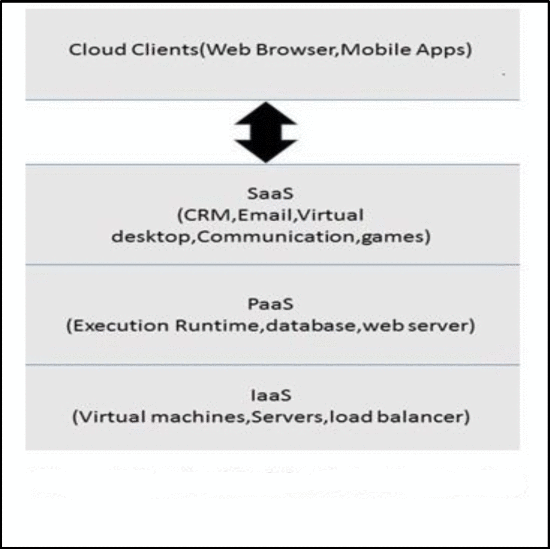
\includegraphics[width=0.75\linewidth]{gambar/Cloud Computing Service Models.png}
    \caption{\textit{Service models} pada \textit{cloud computing}}
    \label{figure:Cloud Computing Service Models}
\end{figure}

Model layanan pada \textit{cloud computing} menentukan tingkat kontrol pengguna atas sumber daya. Model pertama adalah \textit{Infrastructure as a Service} (IaaS), yang menyediakan entitas komputasi esensial seperti jaringan, penyimpanan, dan sumber daya komputasi lainnya. Pada model ini, pengguna tidak mengelola infrastruktur fisik \textit{cloud}, tetapi memiliki kontrol penuh atas sistem operasi, penyimpanan, dan aplikasi yang diimplementasikan, serta beberapa komponen jaringan tertentu. Model kedua, \textit{Platform as a Service} (PaaS), menyediakan platform berupa perangkat keras dan perangkat lunak yang dibutuhkan pengguna untuk mengembangkan dan menjalankan aplikasinya. Penyedia layanan mengelola infrastruktur secara keseluruhan, sehingga pengguna tidak perlu mengadakan perangkat keras atau perangkat lunak internal dan dapat fokus pada siklus pengembangan aplikasi. Model ketiga adalah \textit{Software as a Service} (SaaS), di mana pengguna dapat langsung mengakses dan menggunakan aplikasi perangkat lunak melalui internet dari berbagai perangkat. Layanan ini dikelola sepenuhnya oleh penyedia, termasuk pembaruan dan pemeliharaan, sehingga dapat diakses kapan saja dan dari mana saja \parencite{Sakshi2016}.

\subsection{\textit{Cloud Task Scheduling}}
\textit{Cloud task scheduling} adalah proses penentuan urutan dan alokasi tugas ke sumber daya komputasi yang tersedia dalam lingkungan \textit{cloud computing} untuk mencapai tujuan tertentu seperti minimalisasi \textit{makespan} (waktu penyelesaian total), peningkatan pemanfaatan sumber daya, dan pengurangan biaya operasi. Penjadwalan tugas merupakan salah satu aspek penting dalam \textit{cloud computing} untuk memastikan bahwa sumber daya komputasi digunakan secara efisien dan efektif \parencite{Awad2022}.

Konsep dasar \textit{cloud computing} menyediakan layanan komputasi melalui internet, yang mencakup infrastruktur, platform, dan aplikasi perangkat lunak. Dalam lingkungan \textit{cloud}, berbagai tugas dari banyak pengguna perlu dijadwalkan secara optimal pada sumber daya komputasi yang tersedia, baik itu mesin fisik maupun mesin virtual. Penjadwalan tugas di \textit{cloud} melibatkan pengelolaan tugas-tugas dari berbagai pengguna untuk menggunakan sumber daya secara efisien dalam lingkungan yang bersifat dinamis dan terdistribusi \parencite{Buyya2009}.

\subsection{\textit{Swarm Intelligence}}
\textit{Swarm Intelligence} adalah pendekatan kecerdasan buatan yang terinspirasi oleh perilaku kolektif dari sistem desentralisasi seperti kawanan burung, koloni semut, dan kawanan ikan. Prinsip dasar dari \textit{Swarm Intelligence} meliputi desentralisasi, interaksi lokal, dan emergensi, di mana perilaku global yang kompleks muncul dari interaksi sederhana antara agen individu. Algoritma yang terkenal dalam \textit{Swarm Intelligence} mencakup \textit{Ant Colony Optimization} (ACO), \textit{Particle Swarm Optimization} (PSO), dan \textit{Artificial Bee Colony} (ABC). Masing-masing algoritma ini meniru mekanisme alamiah untuk memecahkan masalah optimasi dengan cara yang adaptif.

Dalam konteks komputasi awan, \textit{Swarm Intelligence} telah diterapkan untuk penjadwalan tugas yang efisien dan penggunaan sumber daya yang optimal. Penelitian oleh Wang Xiang dan Wang Yancheng menunjukkan bahwa algoritma \textit{Swarm Intelligence}, seperti PSO dan ABC dapat secara signifikan meningkatkan efisiensi penjadwalan tugas di lingkungan \textit{cloud} dengan memperkenalkan strategi optimasi multi-objektif dan fungsi \textit{fitness} yang diperbaiki \parencite{Xiang2023}. Selain itu, algoritma ABC yang telah ditingkatkan menunjukkan kinerja yang lebih baik dalam hal mengurangi \textit{makespan} dan penyeimbangan beban pada mesin virtual di lingkungan \textit{cloud} yang heterogen \parencite{Kimpan2016}. \textit{Swarm Intelligence} menawarkan solusi yang adaptif dan efektif untuk berbagai tantangan kompleks dalam dunia komputasi awan.

\subsection{\textit{Artificial Bee Colony}}
\textit{Artificial Bee Colony} (ABC) adalah sebuah algoritma optimasi yang mekanismenya terinspirasi dari perilaku koloni lebah madu dalam mencari makan. Dalam analogi yang digunakan pada algoritma ini, posisi sumber makanan di alam direpresentasikan sebagai kandidat solusi dalam sebuah ruang pencarian. Koloni lebah di dalam algoritma ini terdiri dari tiga jenis lebah, yaitu \textit{employed bees} (lebah pekerja), \textit{onlooker bees} (lebah pengamat), dan \textit{scout bees} (lebah pengintai) \parencite{Wang2021}.

Setiap fase dalam algoritma ABC, memiliki rumus khusus yang digunakan untuk memodifikasi posisi solusi berdasarkan interaksi antara koloni lebah. Fase pertama dalam algoritma ini adalah fase \textit{employed bees}, di mana lebah pekerja mencari solusi yang lebih baik di sekitar solusi yang sedang dieksplorasi. Pada persamaaan \ref{equation:Fase Employed Bees ABC} menghitung posisi solusi baru.

\begin{equation}
\label{equation:Fase Employed Bees ABC}
    v_{mi} = x_{mi} + \varphi_{mi} \cdot (x_{mi} - x_{ki})
\end{equation}

Di mana \(v_{mi}\) adalah posisi sumber makanan baru yang dihasilkan, \(x_{mi}\) adalah posisi sumber makanan yang sedang dieksplorasi, \(x_{ki}\) adalah sumber makanan tetangga yang dipilih secara acak, \(\varphi_{mi}\) adalah nilai acak yang berada dalam rentang \([-a, a]\), dan \(a\) adalah parameter yang mengontrol ruang pencarian. Setelah menghasilkan sumber makanan baru, nilai \textit{fitness} dari solusi \(v_{mi}\) dihitung dan seleksi dengan metode \textit{greedy} yang diterapkan antara solusi \(v_{mi}\) dan \(x_{mi}\) untuk memilih solusi terbaik \parencite{Karaboga2010}.

Pada fase \textit{onlooker bees}, koloni lebah terdiri dari dua kelompok, yaitu lebah pengamat dan lebah pengintai. Lebah pekerja berbagi informasi mengenai sumber makanan yang mereka temukan dengan lebah pengamat yang berada di dalam sarang. Berdasarkan informasi ini, lebah pengamat kemudian memilih sumber makanan dengan probabilitas yang dihitung berdasarkan nilai \textit{fitness} yang diberikan oleh lebah pekerja. Untuk keperluan ini, digunakan metode seleksi berbasis \textit{fitness}, seperti seleksi roda \textit{roulette}, di mana nilai \textit{fitness} sumber makanan menjadi faktor utama dalam pemilihan solusi. Probabilitas \(p_{mi}\) dengan mana sumber makanan \(x_m\) dipilih oleh lebah pengamat dapat dihitung dengan menggunakan persamaan \ref{equation:Fase Onlooker Bees ABC} \parencite{Karaboga2010}.

\begin{equation}
\label{equation:Fase Onlooker Bees ABC}
    p_m = \frac{\text{fit}_m(x_m)}{\sum_{m=1}^{SN} \text{fit}_m(x_m)}
\end{equation}

Di mana \(\text{fit}_m(x_m)\) adalah nilai \textit{fitness} dari sumber makanan \(x_m\) pada iterasi ke-\(m\), dan \(SN\) adalah ukuran populasi sumber makanan. Setelah sumber makanan \(x_m\) dipilih secara probabilistik oleh lebah pengamat, sebuah sumber makanan tetangga \(v_m\) ditentukan menggunakan persamaan \ref{equation:Fase Employed Bees ABC}, dan nilai \textit{fitness} nya dihitung.

Pada fase \textit{scout bees}, lebah yang tidak dapat meningkatkan solusi mereka melalui sejumlah percobaan yang telah ditentukan, yang disebut dengan \textit{limit}, akan bertransformasi menjadi lebah pengintai. Lebah pekerja yang solusinya tidak dapat diperbaiki dalam jumlah percobaan yang telah ditetapkan oleh pengguna algoritma ABC, akan dianggap sebagai lebah pengintai, dan solusi yang mereka bawa akan ditinggalkan. Setelah itu, lebah pengintai mulai mencari solusi baru secara acak. Misalnya, jika solusi \( x_m \) telah ditinggalkan, solusi baru yang ditemukan oleh lebah pengintai yang sebelumnya merupakan lebah pekerja dari \( x_m \) akan menggantikan solusi yang telah ditinggalkan tersebut. Proses ini memastikan bahwa solusi yang awalnya buruk atau telah menjadi buruk akibat eksploitasi, akan digantikan dengan solusi baru yang lebih baik, menghindari terjebaknya algoritma dalam solusi yang tidak optimal \parencite{Karaboga2010}. 

ABC telah diterapkan dalam berbagai masalah optimasi, termasuk penjadwalan tugas di \textit{cloud}. Algoritma ini menunjukkan kemampuan untuk menemukan solusi global dan menghindari perangkap lokal, yang menjadikannya cocok untuk lingkungan komputasi yang dinamis dan kompleks. Penelitian yang dilakukan oleh Warangkhana Kimpan dan Boonhatai Kruekaew menunjukkan bahwa algoritma ABC dapat digunakan untuk penjadwalan tugas pada mesin virtual di \textit{cloud computing}. Mereka memperkenalkan \textit{heuristic task scheduling} dengan algoritma ABC untuk mesin virtual dalam lingkungan \textit{cloud} yang heterogen. Hasil eksperimen menunjukkan bahwa penggunaan ABC dapat meningkatkan efisiensi penjadwalan tugas dan penyeimbangan beban mesin virtual, serta meminimalkan \textit{makespan} \parencite{Kimpan2016}.

\subsection{\textit{Particle Swarm Optimization} (PSO)}
\textit{Particle Swarm Optimization} (PSO) merupakan algoritma optimasi yang dirancang untuk menyelesaikan masalah optimasi kontinu. Berbeda dengan algoritma genetika (\textit{Genetic Algorithm}) yang terinspirasi dari teori evolusi Darwin, PSO mengambil inspirasi dari perilaku sosial kawanan burung dalam mencari lokasi pendaratan terbaik. Dalam konteks ini, gerakan partikel dalam PSO diibaratkan sebagai kawanan burung yang secara sinkron bergerak untuk menentukan tempat pendaratan yang optimal dengan mempertimbangkan berbagai faktor, seperti ketersediaan makanan atau risiko predator. Karena terinspirasi oleh perilaku sosial, PSO diklasifikasikan sebagai bagian dari algoritma \textit{Swarm Intelligence} \parencite{Vanneschi2023}.

\subsection{\textit{Genetic Algorihm} (GA)}
\textit{Genetic Algorithm} (GA) merupakan keluarga model komputasi yang terinspirasi oleh proses evolusi biologis. Algoritma ini merepresentasikan solusi potensial untuk suatu masalah dalam bentuk struktur data yang menyerupai kromosom sederhana. GA menggunakan operator rekombinasi untuk memanipulasi struktur ini dengan tujuan mempertahankan informasi penting yang dapat meningkatkan kualitas solusi. Proses GA dimulai dengan inisialisasi populasi yang terdiri dari kromosom-kromosom yang biasanya dipilih secara acak. Setiap kromosom dievaluasi untuk menentukan tingkat kecocokan \textit{fitness} terhadap masalah yang dihadapi. Berdasarkan evaluasi tersebut, kromosom yang mewakili solusi yang lebih baik mendapatkan peluang reproduksi yang lebih besar dibandingkan dengan kromosom yang kualitasnya lebih rendah. Dengan cara ini, GA secara bertahap mengarahkan populasi menuju solusi yang lebih optimal melalui mekanisme seleksi alam dan rekombinasi \parencite{Mathew2019}.

\subsection{CloudSim}
CloudSim adalah \textit{toolkit} simulasi yang dirancang untuk memodelkan dan mensimulasikan lingkungan komputasi awan. Dikembangkan oleh Buyya, CloudSim menyediakan platform bagi peneliti untuk menguji dan mengevaluasi berbagai algoritma penjadwalan sumber daya dan teknik manajemen tanpa memerlukan infrastruktur \textit{cloud} fisik. Ini memungkinkan eksperimen dilakukan dalam lingkungan yang terkendali dan hasilnya dapat direplikasi dengan mudah. CloudSim terdiri dari beberapa komponen utama seperti \textit{data center}, \textit{host}, \textit{virtual machine} (VM), \textit{cloudlet}, dan broker, yang semuanya bekerja sama untuk memodelkan infrastruktur dan layanan \textit{cloud} secara efisien \parencite{Buyya2009}.

Salah satu keunggulan CloudSim adalah kemampuannya untuk mensimulasikan berbagai skenario komputasi awan, termasuk pengelolaan beban kerja yang dinamis dan heterogen. Selain itu, CloudSim mendukung perluasan dan modifikasi, memungkinkan peneliti untuk menambahkan fungsionalitas baru atau menyesuaikan perilaku komponen yang ada sesuai dengan kebutuhan spesifik mereka. Penelitian oleh Long dan Zhao memperluas CloudSim dengan menambahkan fungsi manajemen replikasi data dan pengelolaan \textit{striping file}, meningkatkan kemampuannya untuk simulasi penyimpanan data \textit{cloud} \parencite{Long2012}. Fitur-fitur baru ini memungkinkan pengguna CloudSim untuk mengintegrasikan strategi manajemen replikasi dan tata letak \textit{file} ke dalam penjadwalan tugas \textit{cloud}, yang berguna untuk meningkatkan kinerja sistem secara keseluruhan.

\subsection{Docker}
Docker adalah sebuah alat yang memungkinkan proses pembuatan artefak aplikasi yang dapat didistribusikan dengan mudah, penerapan aplikasi secara skala besar di berbagai lingkungan, serta memperlancar alur kerja dan responsifitas organisasi pengembangan perangkat lunak yang mengadopsi metodologi \textit{agile}. Dengan Docker, aplikasi dan seluruh dependensinya dikemas dalam sebuah \textit{container} yang portabel dan terisolasi, sehingga dapat dijalankan konsisten di berbagai platform perangkat keras dan sistem operasi \parencite{Matthias2015}.

Pemilihan Docker sebagai alat \textit{containerization} dalam studi ini didasarkan pada kesederhanaannya, portabilitas yang tinggi, dukungan komunitas yang kuat, serta pangsa pasar yang dominan di bidang \textit{containerization} \parencite{Novotny2023}.

\subsection{\textit{Elite Opposition-Based Learning}}
\textit{Elite Opposition-Based Learning} (EOBL) adalah teknik optimasi yang dikembangkan untuk meningkatkan kinerja algoritma optimasi dengan memanfaatkan konsep pembelajaran berbasis oposisi. Teknik ini berfokus pada penggunaan solusi oposisi dari individu \textit{elite} terpilih dalam populasi saat ini untuk mempercepat konvergensi algoritma menuju solusi optimal. Dalam EOBL, solusi oposisi dihitung untuk beberapa individu \textit{elite} pada probabilitas tertentu, dan populasi oposisi yang dihasilkan bersaing dengan populasi asli untuk memberikan lebih banyak peluang menemukan solusi global\parencite{Rahnamayan2008}.

Penggunaan \textit{Elite Opposition-Based Learning} (EOBL) dalam optimasi penjadwalan tugas di lingkungan \textit{cloud} dapat meningkatkan keberagaman solusi dengan memanfaatkan konsep \textit{generation jumping}, yaitu mengatur probabilitas terjadinya operasi oposisi sebagai pola mutasi untuk mendorong eksplorasi solusi yang lebih luas. EOBL mengutamakan penggunaan individu \textit{elite} dari populasi saat ini, menggantikan individu biasa pada OBL konvensional, sehingga solusi oposisi yang dihasilkan lebih mungkin berada di wilayah yang lebih baik dan mendekati solusi global optimal. Pendekatan ini memungkinkan algoritma untuk mempercepat konvergensi menuju solusi optimal, membantu menghindari jebakan pada solusi lokal, dan secara potensial meningkatkan efisiensi dalam penjadwalan tugas seperti pengurangan \textit{imbalance degree} \parencite{Zhou2013}.

\subsection{\textit{Dataset The san Diego Supercomputer} (SDSC) \textit{Blue Horizon Log}}
\textit{Dataset San Diego Supercomputer Center} (SDSC) \textit{Blue Horizon Log} merupakan kumpulan data rekaman jejak tugas (\textit{job trace}) yang dikumpulkan dari sistem Cray X-MP yang menjalankan sistem operasi CTSS pada bulan Oktober dan November 1989. Dataset ini mencakup lebih dari satu juta catatan tugas yang berisi informasi nama tugas, waktu mulai dan selesai, serta statistik pemakaian sumber daya seperti waktu CPU, waktu saluran input/\textit{output}, dan produk ruang-waktu memori. Untuk analisis, tugas-tugas diklasifikasikan berdasarkan nama perintah yang dijalankan, yang dibedakan menjadi perintah publik (dapat diakses oleh semua pengguna) dan perintah privat (khusus untuk pengguna tertentu). Karakterisasi statis dari dataset dilakukan dengan membuat representasi tugas rata-rata untuk setiap perintah, yang mewakili konsumsi sumber daya rata-rata dari seluruh tugas dengan nama perintah tersebut. Selanjutnya, tugas representatif ini diberi bobot sesuai dengan frekuensi relatif kemunculannya dalam keseluruhan data. Agar data lebih homogen dan \textit{outlier} dapat terisolasi, dilakukan transformasi logaritmik dan penskalaan. Data kemudian dikelompokkan menggunakan algoritma klaster \textit{k-means} dengan jarak \textit{euclidean} berbobot, mempertimbangkan tiga parameter utama pemakaian sumber daya, yaitu waktu CPU, waktu input/\textit{output}, dan produk ruang-waktu memori. Hasil klasterisasi ini membagi tugas menjadi tujuh klaster yang menggambarkan pola penggunaan sumber daya yang berbeda dalam sistem SDSC \textit{Blue Horizon} \parencite{Pasquale1988}.

\subsection{Parameter Penggunaan Sumber Daya \textit{Cloud}}
Beberapa parameter yang digunakan untuk menilai efisiensi dan kinerja sistem \textit{task scheduling} dalam pemanfaatan sumber daya \textit{cloud}.
\subsubsection{A. \textit{Makespan}}
\textit{Makespan} adalah interval waktu antara dimulainya tugas pertama hingga selesainya tugas terakhir dalam suatu proses penjadwalan. Nilai \textit{makespan} yang lebih kecil menunjukkan kinerja sistem yang lebih baik karena tugas dapat diselesaikan lebih cepat. Secara matematis, \textit{makespan} dinyatakan sebagai waktu penyelesaian maksimum dari seluruh tugas seperti pada persamaan \ref{equation:Makespan}.

\begin{equation}
\label{equation:Makespan}
    \text{\textit{Makespan}} = \max_{i \in \text{\textit{tasks}}} \{F_i\}
\end{equation}

Di mana $F_i$ adalah waktu penyelesaian (\textit{finishing time}) dari tugas ke-$i$ \parencite{Ciptaningtyas2024}.

\subsubsection{B. \textit{Average Start Time}}
\textit{Average start time} (waktu mulai rata-rata) adalah durasi rata-rata yang diperlukan untuk memulai pemrosesan semua tugas dalam sistem. Waktu mulai yang lebih awal menunjukkan efisiensi yang lebih baik dalam penjadwalan tugas. \textit{Average start time} dapat dihitung seperti pada persamaan \ref{equation:Average Start Time}.

\begin{equation}
\label{equation:Average Start Time}
    \text{\textit{Average start time}} = \frac{\sum_{i=1}^{n} \text{\textit{start time of} } R_i}{nR}
\end{equation}

Di mana $R_i$ adalah sumber daya ke-$i$, dan $nR$ adalah jumlah total sumber daya \parencite{Ciptaningtyas2024}.

\subsubsection{C. \textit{Average Finish Time}}
\textit{Average finish time} (waktu selesai rata-rata) adalah durasi rata-rata yang dibutuhkan untuk menyelesaikan seluruh tugas secara sukses. Waktu selesai yang lebih awal menunjukkan kinerja penjadwalan yang lebih baik. \textit{Average finish time} dapat dihitung seperti pada persamaan \ref{equation:Average Finish Time}.

\begin{equation}
\label{equation:Average Finish Time}
    \text{\textit{Average finish time}} = \frac{\sum_{i=1}^{n} \text{\textit{finish time of} } R_i}{nR}
\end{equation}

Di mana $R_i$ adalah sumber daya ke-$i$ dan $nR$ adalah jumlah total sumber daya \parencite{Ciptaningtyas2024}.

\subsubsection{D. \textit{Average Execution Time}}
\textit{Average execution time} (waktu eksekusi rata-rata) mengacu pada durasi rata-rata yang dibutuhkan untuk menyelesaikan suatu tugas tertentu. Waktu eksekusi yang lebih pendek menunjukkan efisiensi yang lebih baik dalam pelaksanaan tugas. \textit{Average execution time} dapat dihitung seperti pada persamaan \ref{equation:Average Execution Time}.

\begin{equation}
\label{equation:Average Execution Time}
    \text{\textit{Average execution time}} = \frac{\sum_{i=1}^{n} \text{times } T_i}{nT}
\end{equation}

Di mana $T_i$ adalah waktu penyelesaian tugas ke-$i$ dan $nT$ adalah jumlah total tugas \parencite{Ciptaningtyas2024}.

\subsubsection{E. \textit{Average Waiting Time}}
\textit{Average waiting time} adalah rata-rata waktu yang dibutuhkan oleh proses untuk menunggu sebelum dieksekusi dalam antrean. Waktu tunggu ini dihitung dari saat proses memasuki antrean hingga proses tersebut benar-benar dimulai. \textit{Average waiting time} memberikan gambaran seberapa efisien sistem dalam menangani antrean, di mana semakin kecil semakin cepat proses dapat dieksekusi setelah masuk antrean \parencite{Belferik2025}. Secara matematis, rumusnya seperti pada persamaan \ref{equation:Average Waiting Time}.

\begin{equation}
\label{equation:Average Waiting Time}
    \text {\textit{Average waiting time}} = \frac{\text{\textit{TotalDelay}}}{n}
\end{equation}

Untuk menghitung \textit{average waiting time}, kita menggunakan rumus yang lebih umum, yaitu dengan menjumlahkan seluruh \textit{waiting time} dari setiap proses dalam antrean, kemudian membaginya dengan jumlah total proses yang ada. 

\subsubsection{F. \textit{Scheduling Length}}
\textit{Scheduling length} merupakan jumlah total waktu penyelesaian seluruh tugas dalam sistem penjadwalan. Parameter ini mengukur keseluruhan durasi yang dihabiskan untuk mengeksekusi semua tugas, sehingga nilai yang lebih kecil menunjukkan efisiensi penjadwalan yang lebih baik. Secara matematis, \textit{scheduling length} ($SL$) dihitung sebagai total penjumlahan waktu penyelesaian semua tugas seperti pada persamaan \ref{equation:Scheduling Length} \parencite{Emara2021}.

\begin{equation}
\label{equation:Scheduling Length}
    \text{\textit{Scheduling length}} = \text {\textit{scheduling time}} + \textit{makespan}
\end{equation}

\subsubsection{G. \textit{Throughput}}
\textit{Throughput} adalah laju maksimum eksekusi tugas dalam satu satuan waktu. Dengan kata lain, \textit{throughput} mengukur jumlah total tugas yang berhasil diselesaikan per unit waktu. Parameter ini penting untuk menilai performa sistem dalam memproses tugas secara efisien. \textit{Throughput} dapat dihitung seperti pada persamaan \ref{equation:Throughput}.

\begin{equation}
\label{equation:Throughput}
    Throughput = \frac{nT}{makespan}
\end{equation}

Di mana $nT$ adalah jumlah total tugas yang diselesaikan dan $makespan$ adalah waktu penyelesaian tugas terakhir. Dengan nilai \textit{throughput} yang lebih tinggi, sistem dianggap mampu menyelesaikan lebih banyak tugas dalam waktu yang lebih singkat \parencite{Emara2021}.

\subsubsection{H. \textit{Resource Utilization}}
\textit{Resource utilization} (pemanfaatan sumber daya) mengukur efektivitas penggunaan sumber daya fisik, seperti CPU dalam sistem komputasi awan. Pemanfaatan CPU pada sumber daya fisik tertentu dihitung dengan menjumlahkan beban kerja dari setiap \textit{virtual machine}(VM) yang ditempatkan di sumber daya tersebut, lalu dibagi dengan kapasitas CPU sumber daya fisik tersebut. Dalam hal ini, VM yang ditempatkan di sumber daya tersebut dianggap memberikan kontribusi pada beban kerja total \parencite{Emara2021}. \textit{Resource utilization} secara matematis dapat dihitung seperti pada persamaan \ref{equation:Resource Utilization}.

\begin{equation}
\label{equation:Resource Utilization}
    \text{\textit{Resource utilization}} = \frac{\sum_{i=1}^{n} \text{\textit{finish time of} } R_i}{\text{\textit{makespan}} \times nR}
\end{equation}

\subsubsection{I. \textit{Energy Consumption}}
\textit{Energy consumption} (konsumsi energi) dalam sistem \textit{cloud computing} mengacu pada jumlah energi yang digunakan oleh sumber daya fisik untuk menjalankan tugas-tugas yang dialokasikan \parencite{Emara2021}.

\subsubsection{J. \textit{Imbalance Degree}}
\textit{Imbalance degree} (derajat ketidakseimbangan) mengukur seberapa merata distribusi beban kerja di antara \textit{virtual machine} (VM) dalam sistem \textit{cloud computing}, berdasarkan kemampuan eksekusi masing-masing VM. Untuk kebijakan penjadwalan yang ideal, nilai \textit{imbalance degree} harus serendah mungkin, karena nilai yang tinggi menunjukkan distribusi beban yang tidak merata yang dapat menyebabkan beban berlebih pada beberapa VM dan beban kurang pada VM lainnya \parencite{Tomar2022}. \textit{Imbalance degree} dapat dihitung seperti pada persamaan \ref{equation:Imbalance Degree}.

\begin{equation}
\label{equation:Imbalance Degree}
    \text{\textit{Imbalance degree}} = \frac{ET_{\max} - ET_{\min}}{ET_{\text{avg}}}
\end{equation}

di mana $ET_{\max}$ adalah waktu maksimum yang dihabiskan oleh VM dalam mengeksekusi semua \textit{cloudlet} yang diberikan, $ET_{\min}$ adalah waktu minimum, dan $ET_{\text{avg}}$ adalah waktu rata-rata eksekusi pada seluruh VM.
\cleardoublepage

% Bab 3 metodologi
\chapter{METODOLOGI}

\section{Metode yang digunakan}
Bab ini akan dijelaskan secara rinci metodologi yang digunakan dalam penelitian. Metodologi ini mencakup langkah-langkah sistematis yang dilakukan mulai dari persiapan data, simulasi dan implementasi algoritma, hingga pengujian dan evaluasi hasil. Sebagai bagian dari perencanaan dan pelaksanaan penelitian, dibuat diagram alur yang menggambarkan tahapan-tahapan penelitian secara sistematis yang dapat dilihat pada gambar \ref{figure:Flowchart Rancangan Metodologi Penelitian}.

\begin{figure} [H]
  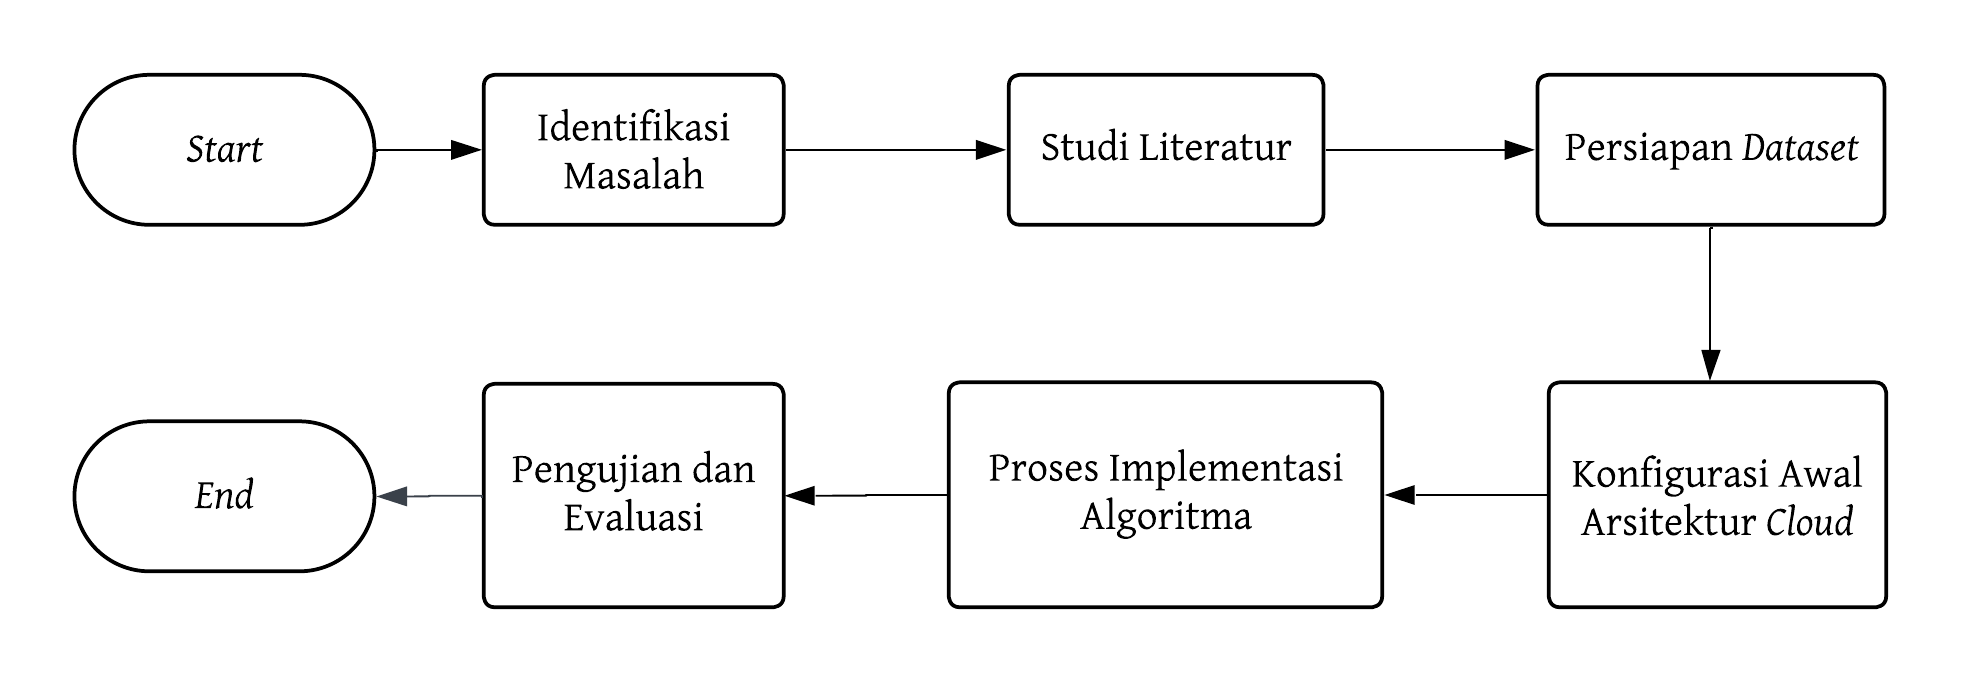
\includegraphics[width=1\linewidth]{gambar/Flowchart Rancangan Metodologi Penelitian.png}
  \caption{Rancangan metodologi penelitian}
  \label{figure:Flowchart Rancangan Metodologi Penelitian}
\end{figure}

\subsection{Identifikasi Masalah}
Penelitian ini mengidentifikasi masalah utama dalam penjadwalan tugas di lingkungan \textit{cloud} yang meliputi kebutuhan untuk memaksimalkan pemanfaatan sumber daya sekaligus mengurangi makespan dan ketidakseimbangan beban kerja antar sumber daya. Algoritma \textit{Artificial Bee Colony} (ABC), meskipun efektif dalam eksplorasi ruang solusi, memiliki keterbatasan pada aspek eksploitasi sehingga sering gagal mengoptimalkan penggunaan sumber daya dan berpotensi terjebak pada solusi lokal yang suboptimal. Kombinasi ABC dengan \textit{Elite Opposition-Based Learning} (EOBL) diharapkan dapat mengatasi permasalahan tersebut dengan meningkatkan eksploitasi dan diversitas populasi, sehingga dapat menghasilkan penjadwalan yang lebih optimal dan efisien.

\subsection{Studi Literatur}
Pada tahap ini, dilakukan studi literatur yang mendalam untuk memahami berbagai pendekatan dan metode yang telah digunakan dalam penjadwalan tugas di lingkungan \textit{cloud computing}. Studi ini mencakup kajian terhadap penelitian-penelitian terdahulu dengan fokus pada kelebihan, kelemahan, serta strategi peningkatan performa seperti studi berbasis oposisi dan penyesuaian parameter dinamis. Selain itu, informasi terkait permasalahan penjadwalan dikumpulkan melalui berbagai sumber referensi, termasuk makalah, buku, dan jurnal yang memiliki relevansi dengan permasalahan penelitian ini. Hasil studi literatur ini menjadi landasan teoritis yang kuat untuk pengembangan algoritma yang lebih efisien serta menjadi acuan dalam merancang metode simulasi dan evaluasi pada penelitian ini.

\subsection{Persiapan \textit{Dataset}}
Penelitian ini menggunakan tiga set data utama. Pertama, SDSC (\textit{San Diego Supercomputer Center}) yang berisi tugas-tugas dari lingkungan superkomputer. \textit{Dataset} ini membutuhkan \textit{preprocessing} untuk mempersiapkan data sebelum digunakan. Kedua, \textit{Simple Random
Dataset}, yang dibuat secara acak menggunakan rumus pada Excel untuk menghasilkan tugas secara acak. Ketiga, \textit{Stratified Random}, yang dihasilkan berdasarkan rentang nilai minimum dan maksimum dari nilai minimum dan maksimum SDSC.

\subsection{Konfigurasi Awal Arsitektur \textit{Cloud}}
\subsubsection{Konfigurasi Awal Simulasi Arsitektur \textit{Cloud}}
Pada tahap ini, \textit{cloud simulator} akan digunakan untuk mengonfigurasi sistem dan mereplikasi skenario pengujian. Kebutuhan penelitian akan menentukan parameter seperti jumlah tugas, kapasitas server, dan distribusi sumber daya. Tujuan utama konfigurasi ini adalah untuk menjamin bahwa lingkungan simulasi secara akurat menggambarkan situasi manajemen sumber daya \textit{cloud} yang sebenarnya. Konfigurasi arsitektur simulasi dapat dilihat pada gambar \ref{figure:Arsitektur Simulasi CloudSim}

\begin{figure} [H]
  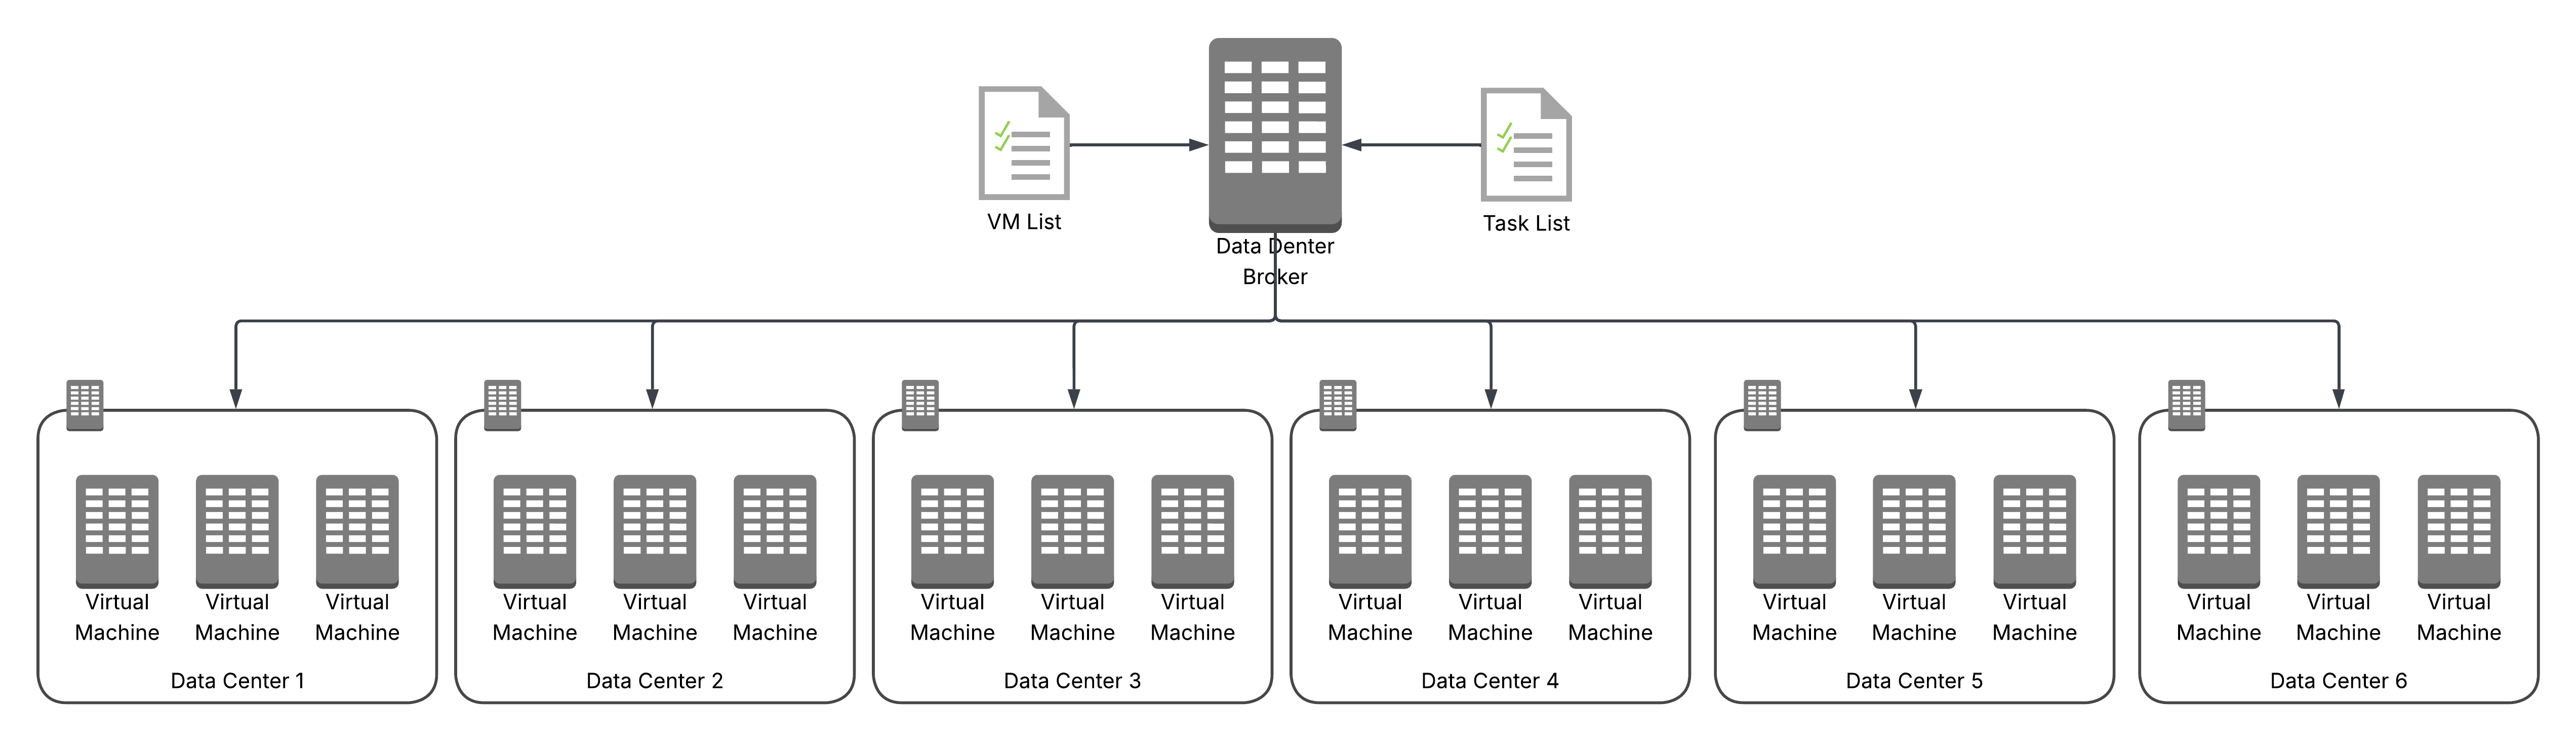
\includegraphics[width=1\linewidth]{gambar/Arsitektur Simulasi CloudSim.png}
  \caption{Arsitektur simulasi CloudSim}
  \label{figure:Arsitektur Simulasi CloudSim}
\end{figure}

Setiap \textit{virtual machine} dan \textit{data center} memiliki spesifikasi masing-masing. Adapun spesifikasi pada tiap sumber daya yang digunakan dalam penelitian ini dapat dilihat dalam tabel \ref{tabel:Spesifikasi Virtual Machine Simulasi}, tabel \ref{tabel:Spesifikasi Host Simulasi}, dan tabel \ref{tabel:Spesifikasi Data Center Simulasi}.

\begin{table} [H]
    \centering
    \caption{Spesifikasi \textit{virtual machine} CloudSim}
    \label{tabel:Spesifikasi Virtual Machine Simulasi}
    \begin{tabular}{|>{\centering\arraybackslash}m{0.1\linewidth}|
                    >{\raggedleft\arraybackslash}m{0.17\linewidth}|
                    >{\raggedleft\arraybackslash}m{0.12\linewidth}|
                    >{\raggedleft\arraybackslash}m{0.15\linewidth}|
                    >{\raggedleft\arraybackslash}m{0.12\linewidth}|
                    >{\raggedleft\arraybackslash}m{0.12\linewidth}|}
        \rowcolor{blue!30}
        \hline
        \multicolumn{1}{|>{\centering\arraybackslash}m{0.1\linewidth}|}{\textbf{ID}} & 
        \multicolumn{1}{>{\centering\arraybackslash}m{0.17\linewidth}|}{\textbf{Memori (MB)}} & 
        \multicolumn{1}{>{\centering\arraybackslash}m{0.12\linewidth}|}{\textbf{RAM (MB)}} & 
        \multicolumn{1}{>{\centering\arraybackslash}m{0.15\linewidth}|}{\textbf{MIPS per Prosesor}} & 
        \multicolumn{1}{>{\centering\arraybackslash}m{0.12\linewidth}|}{\textbf{Jumlah Prosesor}} & 
        \multicolumn{1}{>{\centering\arraybackslash}m{0.12\linewidth}|}{\textbf{Tipe VM}} \\
        \hline
        VM1 & 1.000 & 512  & 400 & 1 & VM 1 \\
        \hline
        VM2 & 1.000 & 1.024 & 500 & 1 & VM 2 \\
        \hline
        VM3 & 1.000 & 2.048 & 600 & 1 & VM 3 \\
        \hline
    \end{tabular}
\end{table}

\newpage

\begin{table} [H]
    \centering
    \caption{Spesifikasi \textit{host} CloudSim}
    \label{tabel:Spesifikasi Host Simulasi}
    \begin{tabular}{|>{\centering\arraybackslash}m{0.07\linewidth}|
                    >{\raggedleft\arraybackslash}m{0.1\linewidth}|
                    >{\raggedleft\arraybackslash}m{0.1\linewidth}|
                    >{\raggedleft\arraybackslash}m{0.1\linewidth}|
                    >{\raggedleft\arraybackslash}m{0.1\linewidth}|
                    >{\raggedleft\arraybackslash}m{0.1\linewidth}|
                    >{\raggedleft\arraybackslash}m{0.1\linewidth}|
                    >{\raggedleft\arraybackslash}m{0.1\linewidth}|}
        \rowcolor{blue!30}
        \hline
        \multicolumn{1}{|>{\centering\arraybackslash}m{0.07\linewidth}|}{\textbf{ID}} & 
        \multicolumn{1}{>{\centering\arraybackslash}m{0.1\linewidth}|}{\textbf{Memori (MB)}} &
        \multicolumn{1}{>{\centering\arraybackslash}m{0.1\linewidth}|}{\textbf{Jumlah \textit{Core}}} &
        \multicolumn{1}{>{\centering\arraybackslash}m{0.1\linewidth}|}{\textbf{Jumlah \textit{Core}}} & 
        \multicolumn{1}{>{\centering\arraybackslash}m{0.1\linewidth}|}{\textbf{MIPS \textit{Core} 1}} & 
        \multicolumn{1}{>{\centering\arraybackslash}m{0.1\linewidth}|}{\textbf{MIPS \textit{Core} 2}} & 
        \multicolumn{1}{>{\centering\arraybackslash}m{0.1\linewidth}|}{\textbf{MIPS \textit{Core} 3}} & 
        \multicolumn{1}{>{\centering\arraybackslash}m{0.1\linewidth}|}{\textbf{MIPS \textit{Core} 4}} \\
        \hline
        H1 & 1.000.000 & 128.000 & 4 & 300 & 400 & 500 & 600 \\
        \hline
        H2 & 1.000.000 & 128.000 & 4 & 300 & 400 & 500 & 600 \\
        \hline
        H3 & 1.000.000 & 128.000 & 4 & 300 & 400 & 500 & 600 \\
        \hline
    \end{tabular}
\end{table}

\begin{table} [H]
    \centering
    \caption{Spesifikasi \textit{data center} CloudSim}
    \label{tabel:Spesifikasi Data Center Simulasi}
    \begin{tabular}{|>{\centering\arraybackslash}m{0.07\linewidth}|
                    >{\raggedleft\arraybackslash}m{0.12\linewidth}|
                    >{\raggedleft\arraybackslash}m{0.1\linewidth}|
                    >{\raggedleft\arraybackslash}m{0.12\linewidth}|
                    >{\raggedleft\arraybackslash}m{0.1\linewidth}|
                    >{\raggedleft\arraybackslash}m{0.15\linewidth}|
                    >{\raggedleft\arraybackslash}m{0.1\linewidth}|}
        \rowcolor{blue!30}
        \hline
        \multicolumn{1}{|>{\centering\arraybackslash}m{0.07\linewidth}|}{\textbf{ID}} & 
        \multicolumn{1}{>{\centering\arraybackslash}m{0.12\linewidth}|}{\textbf{Memori (MB)}} &
        \multicolumn{1}{>{\centering\arraybackslash}m{0.1\linewidth}|}{\textbf{RAM (MB)}} &
        \multicolumn{1}{>{\centering\arraybackslash}m{0.12\linewidth}|}{\textbf{Jumlah Prosesor}} &
        \multicolumn{1}{>{\centering\arraybackslash}m{0.1\linewidth}|}{\textbf{Jumlah \textit{Host}}} & 
        \multicolumn{1}{>{\centering\arraybackslash}m{0.15\linewidth}|}{\textbf{\textit{Bandwidth} (Gbps)}} & 
        \multicolumn{1}{>{\centering\arraybackslash}m{0.1\linewidth}|}{\textbf{\textit{Latency} (ms)}}  \\
        \hline
        D1 & 100.000 & 128 & 6 & 3 & 10 & 6 \\
        \hline
        D2 & 100.000 & 128 & 6 & 3 & 10 & 6 \\
        \hline
        D3 & 100.000 & 128 & 6 & 3 & 10 & 8 \\
        \hline
        D4 & 100.000 & 128 & 6 & 3 & 10 & 8 \\
        \hline
        D5 & 100.000 & 128 & 6 & 3 & 10 & 10 \\
        \hline
        D6 & 100.000 & 128 & 6 & 3 & 10 & 10 \\
        \hline
    \end{tabular}
\end{table}


\subsubsection{Konfigurasi Awal Implementasi \textit{Real} Arsitektur \textit{Cloud}}
Implementasi \textit{real} arsitektur \textit{cloud} pada penelitian ini menggunakan empat buah \textit{virtual machine} (VM) yang berfungsi sebagai lingkungan uji coba. Dari keempat VM tersebut, satu VM berperan sebagai broker yang bertugas sebagai pusat kendali dalam sistem. Broker ini bertanggung jawab untuk menjalankan algoritma optimasi \textit{scheduling} yang digunakan untuk menentukan distribusi task secara efisien ke VM lainnya.

Tiga VM lainnya berperan sebagai \textit{host}, yang masing-masing menjalankan dua \textit{container} berbasis Docker. Dengan konfigurasi ini, total terdapat enam \textit{container}. \textit{Container-container} ini bertugas menjalankan \textit{task} yang telah didistribusikan oleh broker. Konfigurasi ini memungkinkan simulasi lingkungan \textit{cloud} yang nyata, sehingga dapat menguji efektivitas algoritma \textit{scheduling} dalam lingkungan terdistribusi.

Gambar \ref{figure:Arsitektur Implementasi Real} memperlihatkan skema arsitektur sistem secara umum yang menggambarkan hubungan antara broker dan \textit{host} serta \textit{container-container} di dalam \textit{host}. Selain itu, spesifikasi \textit{hardware} dari masing-masing VM yang digunakan pada \textit{real environment} dapat dilihat pada tabel \ref{tabel:Spesifikasi VM Real Environment} dan tabel \ref{tabel:Spesifikasi Broker dan Host Real Environment}, yang menjelaskan secara rinci konfigurasi sumber daya yang digunakan, seperti CPU, RAM, dan penyimpanan.

\newpage

\begin{figure} [H]
  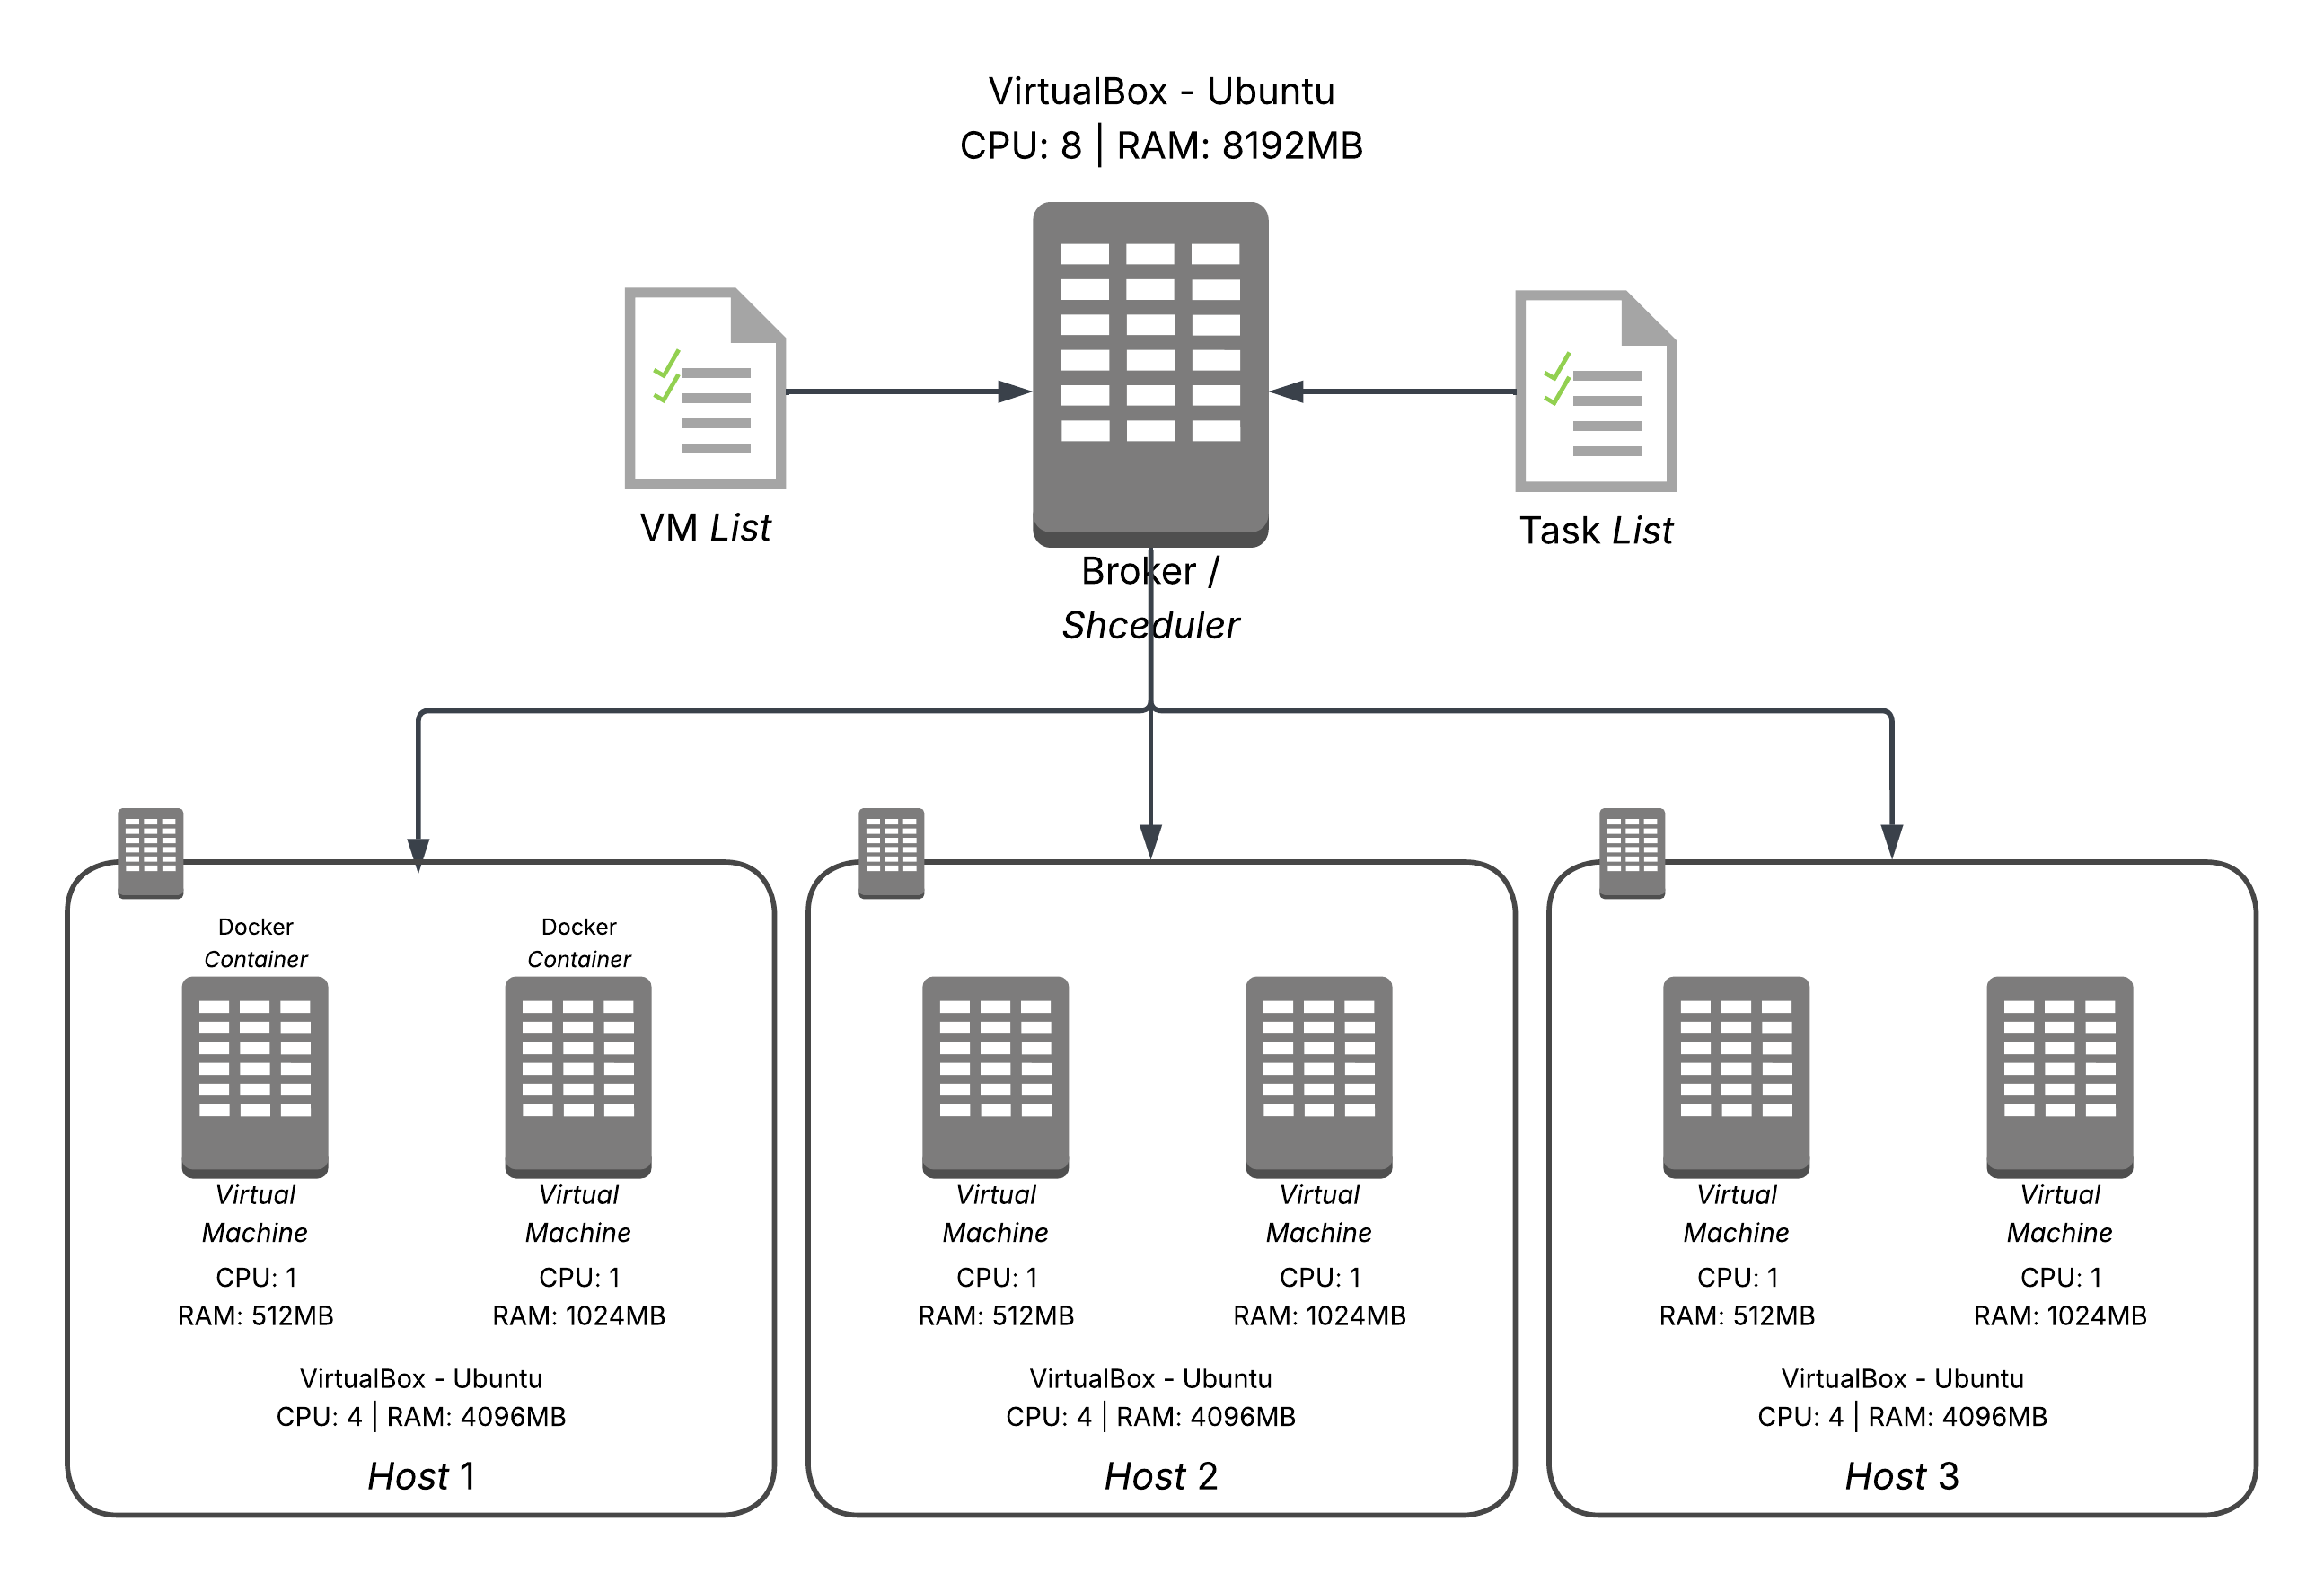
\includegraphics[width=1.1\linewidth]{gambar/Arsitektur Implementasi CloudSim.png}
  \caption{Arsitektur \textit{real environment}}
  \label{figure:Arsitektur Implementasi Real}
\end{figure}

Setiap \textit{virtual machine} dan broker memiliki spesifikasi masing-masing. Adapun spesifikasi pada tiap sumber daya yang digunakan dalam penelitian ini dapat dilihat dalam tabel \ref{tabel:Spesifikasi VM Real Environment}, dan tabel \ref{tabel:Spesifikasi Broker dan Host Real Environment}.

\begin{table} [H]
    \centering
    \caption{Spesifikasi \textit{virtual machine real environment}}
    \label{tabel:Spesifikasi VM Real Environment}
    \begin{tabular}{|>{\centering\arraybackslash}m{0.15\linewidth}|
                    >{\raggedleft\arraybackslash}m{0.20\linewidth}|
                    >{\raggedleft\arraybackslash}m{0.15\linewidth}|}
    \rowcolor{blue!30}
        \hline
        \multicolumn{1}{|>{\centering\arraybackslash}m{0.15\linewidth}|}{\textbf{ID}} & 
        \multicolumn{1}{>{\centering\arraybackslash}m{0.20\linewidth}|}{\textbf{RAM (MB)}} &
        \multicolumn{1}{>{\centering\arraybackslash}m{0.15\linewidth}|}{\textbf{CPU}} \\
        \hline
        VM1 & 512 & 1 \\
        \hline
        VM2 & 1024 & 1 \\
        \hline
    \end{tabular}
\end{table}

\begin{table} [H]
    \centering
    \caption{Spesifikasi broker dan \textit{host real environment}}
    \label{tabel:Spesifikasi Broker dan Host Real Environment}
    \begin{tabular}{|>{\centering\arraybackslash}m{0.2\linewidth}|
                    >{\raggedleft\arraybackslash}m{0.2\linewidth}|
                    >{\raggedleft\arraybackslash}m{0.15\linewidth}|}
    \rowcolor{blue!30}
        \hline
        \multicolumn{1}{|>{\centering\arraybackslash}m{0.2\linewidth}|}{\textbf{ID}} & 
        \multicolumn{1}{>{\centering\arraybackslash}m{0.2\linewidth}|}{\textbf{RAM (MB)}} &
        \multicolumn{1}{>{\centering\arraybackslash}m{0.15\linewidth}|}{\textbf{CPU}} \\
        \hline
        Broker & 8192 & 8 \\
        \hline
        Host 1 & 4096 & 4 \\
        \hline
        Host 2 & 4096 & 4 \\
        \hline
        Host 3 & 4096 & 4 \\
        \hline
    \end{tabular}
\end{table}

\newpage

\subsection{Implementasi Algoritma}
Tahap implementasi dilakukan setelah desain dan konfigurasi sistem selesai. Pada tahap ini, \textit{pseudocode} yang telah di analisa sebelumnya diubah menjadi program yang dapat dijalankan pada platform CloudSim. Penelitian ini mengimplementasikan algoritma \textit{Artificial Bee Colony} (ABC) yang dikombinasikan dengan metode \textit{Elite Opposition-Based Learning} (EOBL). 

\begin{table} [H]
    \centering
    \caption{\textit{Pseudocode} dari proses \textit{Artificial Bee Colony} (ABC)}
    \begin{tabular}{|p{0.95\linewidth}|}
    \hline
    \textbf{Input:} Daftar tugas (\textit{task/cloudlets}) dan daftar \textit{virtual machine} (VM). \\
    \textbf{\textit{Output}:} Solusi terbaik dari alokasi tugas. \\
    \textbf{Langkah:} 
    \begin{enumerate}[leftmargin=*,label=\arabic*.,itemsep=0pt,parsep=0pt]
        \item Mulai.
        \item Tetapkan iterasi $t = 1$.
        \item Definisikan dimensi masalah.
        \item Hasilkan populasi awal.
        \item Evaluasi \textit{fitness} dari setiap individu.
        \item \textbf{\textit{while}} kondisi terminasi belum terpenuhi \textbf{\textit{do}}
        \item \hspace{1em} Untuk setiap lebah pekerja (\textit{employed bees}) \textbf{\textit{do}}
        \item \hspace{2em} Temukan sumber makanan baru dan evaluasi \textit{fitness}.
        \item \hspace{2em} Terapkan mekanisme seleksi \textit{greedy}.
        \item \hspace{1em} \textbf{\textit{end for}}
        \item \hspace{1em} Hitung probabilitas untuk setiap sumber makanan.
        \item \hspace{1em} Untuk setiap lebah pengamat (\textit{onlooker bees}) \textbf{\textit{do}}
        \item \hspace{2em} Pilih sumber makanan.
        \item \hspace{2em} Hasilkan sumber makanan baru.
        \item \hspace{2em} Evaluasi \textit{fitness}.
        \item \hspace{2em} Terapkan mekanisme seleksi \textit{greedy}.
        \item \hspace{1em} \textbf{\textit{end for}}
        \item \hspace{1em} Fase lebah pengintai (\textit{scout bees}):
        \item \hspace{2em} \textbf{\textit{if}} ada lebah pekerja yang menjadi lebah pengintai \textbf{then}
        \item \hspace{3em} Kirim lebah pengintai ke sumber makanan acak.
        \item \hspace{2em} \textbf{\textit{end if}}
        \item \hspace{1em} Set iterasi $t = t + 1$.
        \item \textbf{\textit{end while}}
        \item Selesai.
    \end{enumerate} \\
    \hline
    \end{tabular}
\end{table}

\newpage

\begin{figure} [H] 
  \centering
  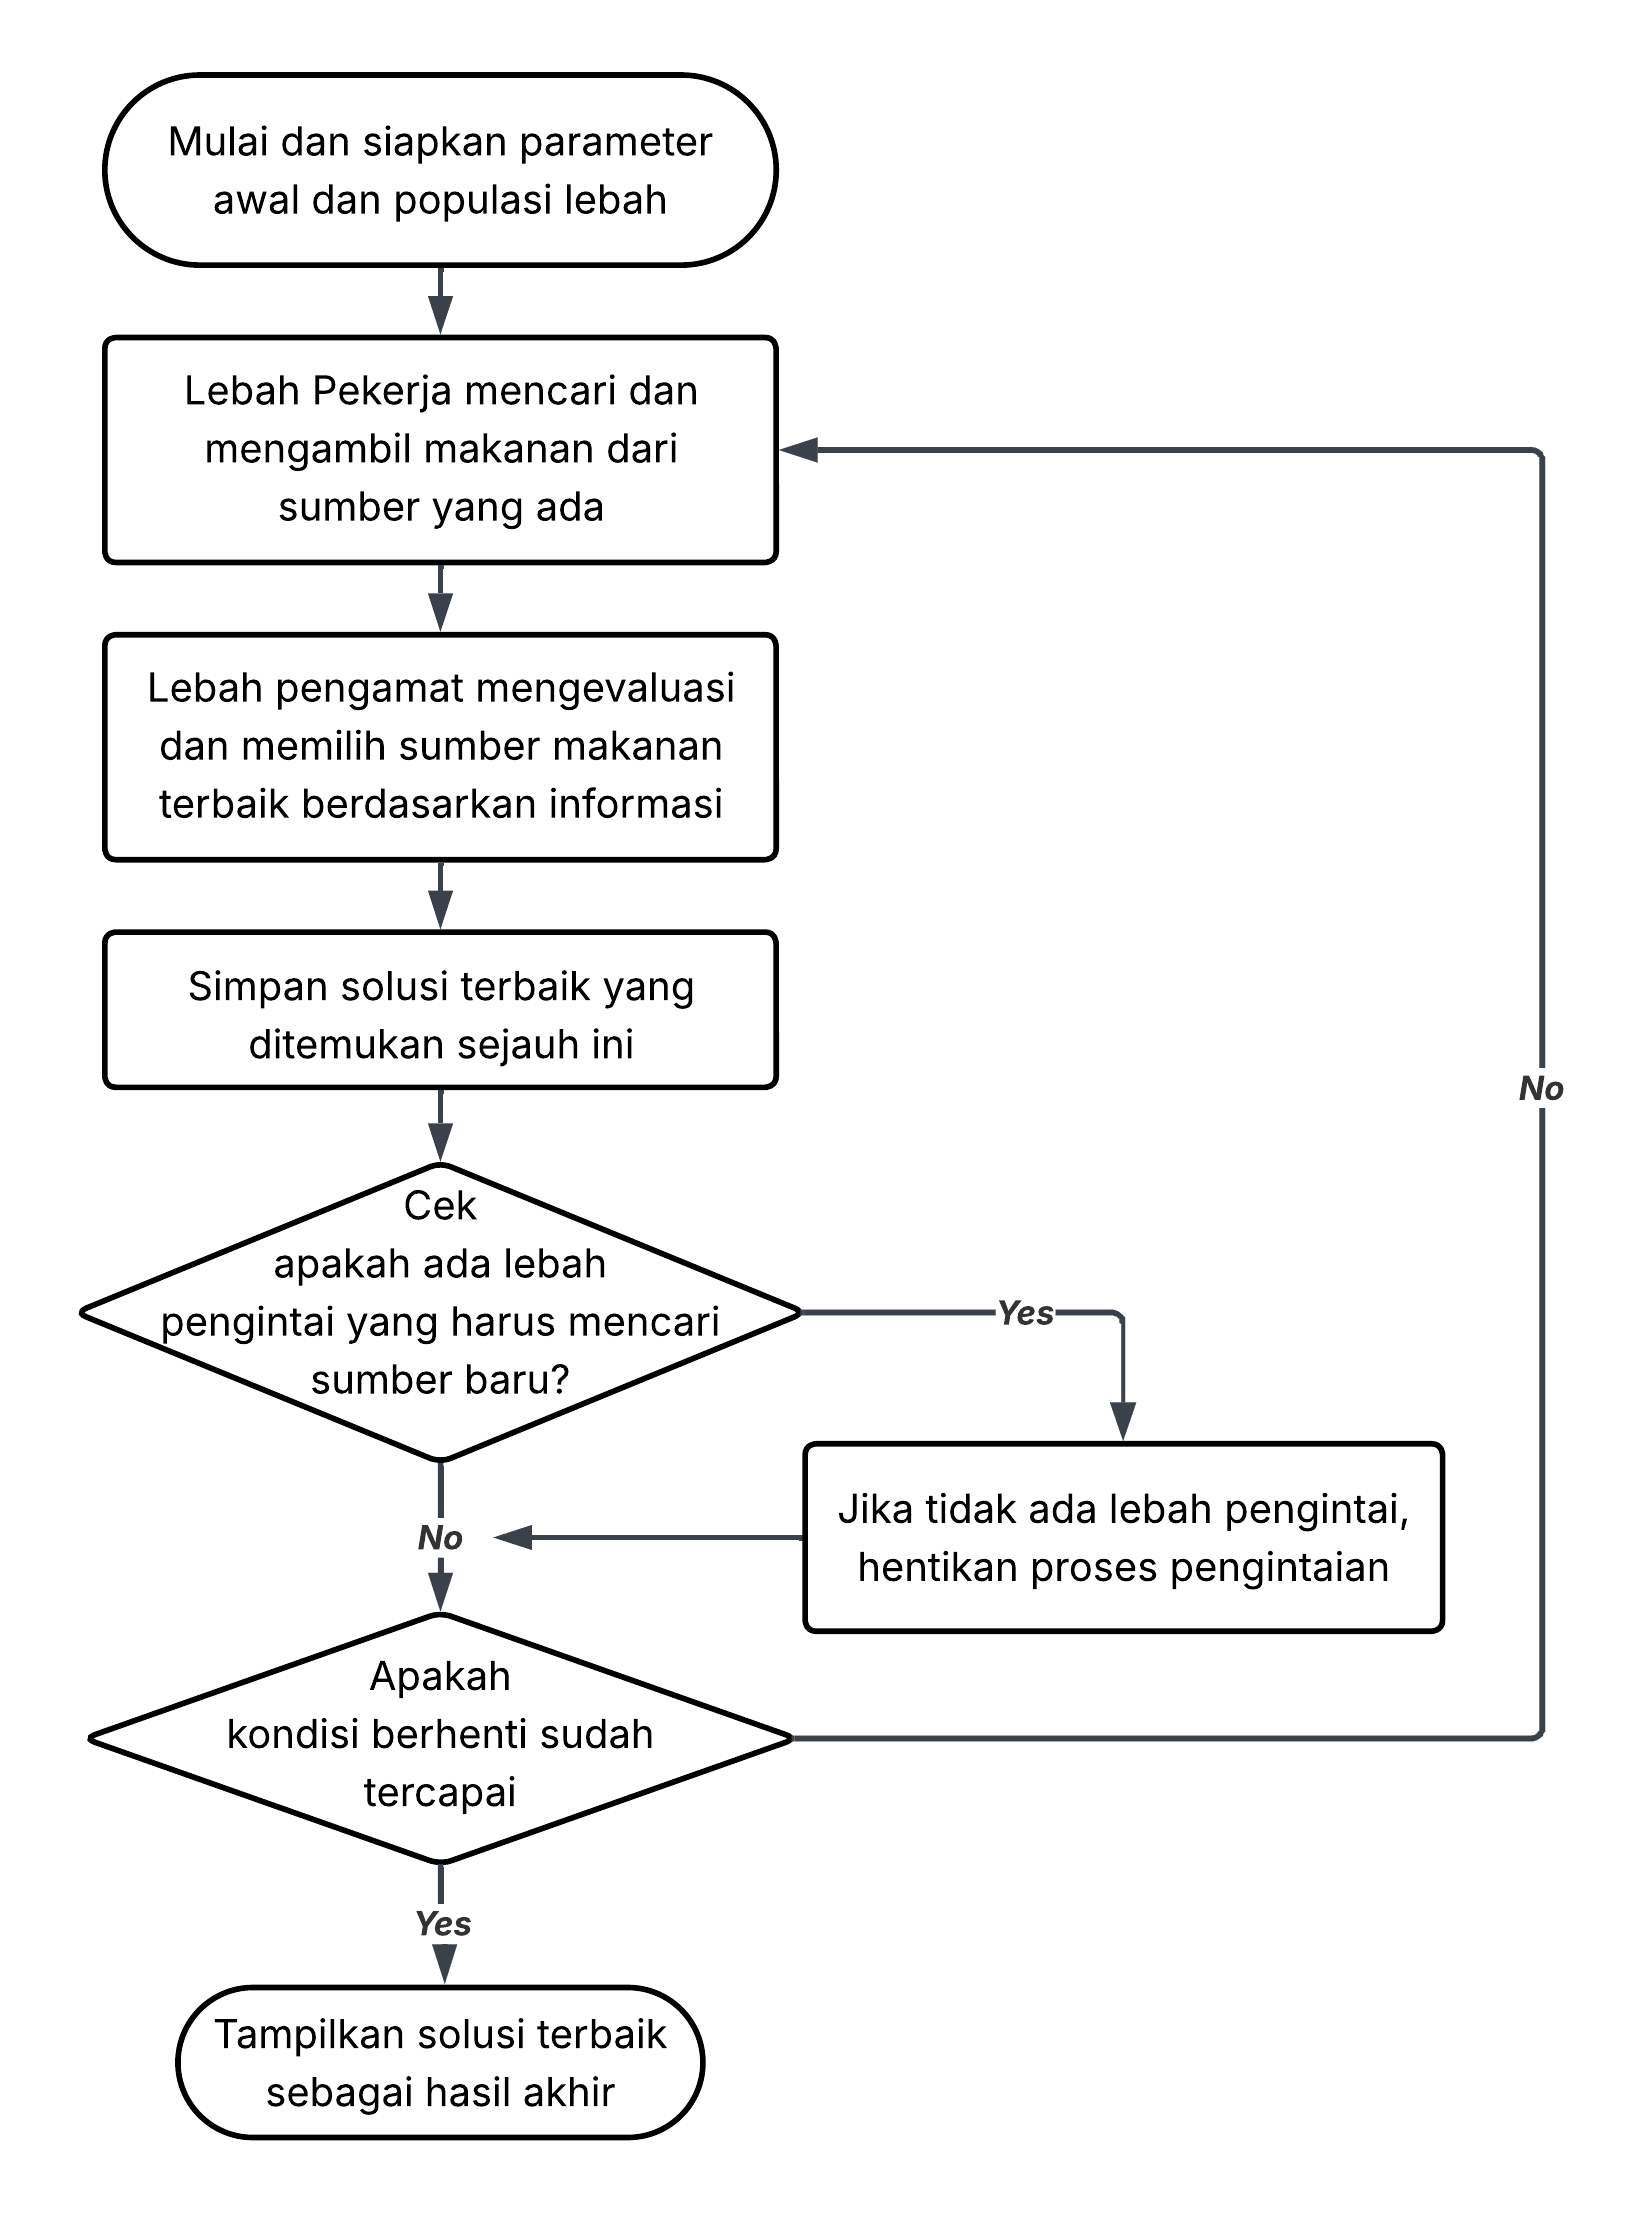
\includegraphics[width=0.85\linewidth]{gambar/Flowchart ABC Algorithm.png}
  \caption{Flowchart dari \textit{Artificial Bee Colony} (ABC)}
  \label{figure:Flowchart ABC Algorithm}
\end{figure}

\begin{table}[H]
    \centering
    \caption{\textit{Pseudocode} proses \textit{Elite Opposition-Based Artificial Bee Colony} (ABC-EOBL)}
    \begin{tabular}{|p{0.95\linewidth}|}
    \hline
    \textbf{Input:} Daftar tugas (\textit{task/cloudlets}) dan daftar \textit{virtual machine} (VM). \\
    \textbf{\textit{Output}:} Solusi terbaik dari alokasi tugas. \\
    \textbf{Langkah:}
    \begin{enumerate}[leftmargin=*, label=\arabic*., itemsep=0pt, parsep=0pt]
        \item Mulai.
        \item Tetapkan iterasi $t = 0$.
        \item Tetapkan evaluasi fungsi $FEs = 0$.
        \item Inisialisasi populasi.
        \item Evaluasi \textit{fitness} setiap individu.
        \item \textbf{\textit{while}} ($FEs < MAX\_FEs$) \textbf{\textit{do}}
        \item \hspace{1em} Hasilkan probabilitas acak $Pr = \text{rand}(0, 1)$.
        \item \hspace{1em} \textbf{\textit{if}} ($Pr < P_e$) \textbf{\textit{then}}
        \item \hspace{2em} Pilih $EN$ solusi \textit{elite} dari populasi saat ini.
        \item \hspace{2em} Hitung batas bawah dan atas ruang pencarian.
        \item \hspace{2em} Inisialisasi populasi \textit{elite opposition} $\mathbf{EOP} = \{\}$.
        \item \hspace{2em} \textbf{\textit{for each}} individu $i$ dalam populasi \textbf{\textit{do}}
        \item \hspace{3em} Hasilkan nilai acak $k = \text{rand}(0, 1)$.
        \item \hspace{3em} Buat solusi \textit{elite opposition} $EO_i$ untuk individu $X_i$.
        \item \hspace{3em} Evaluasi \textit{fitness} $EO_i$.
        \item \hspace{3em} Tambahkan $EO_i$ ke populasi \textit{opposition}: $\mathbf{EOP} = \mathbf{EOP} \cup \{EO_i\}$.
        \item \hspace{3em} Tambahkan evaluasi fungsi: $FEs = FEs + 1$.
        \item \hspace{2em} \textbf{\textit{end for}}
        \item \hspace{2em} Gabungkan populasi $P$ dan populasi \textit{opposition} $\mathbf{EOP}$.
        \item \hspace{2em} Pilih $SN$ solusi terbaik untuk generasi berikutnya.
        \item \hspace{1em} \textbf{else}
        \item \hspace{2em} Jalankan algoritma ABC.
        \item \hspace{1em} \textbf{\textit{end if}}
        \item \hspace{1em} Tetapkan iterasi $t = t + 1$.
        \item \textbf{\textit{end while}}
        \item Kembalikan solusi terbaik yang ditemukan.
        \item Selesai.
    \end{enumerate} \\
    \hline
    \end{tabular}
\end{table}

\begin{figure} [H]
    \centering
    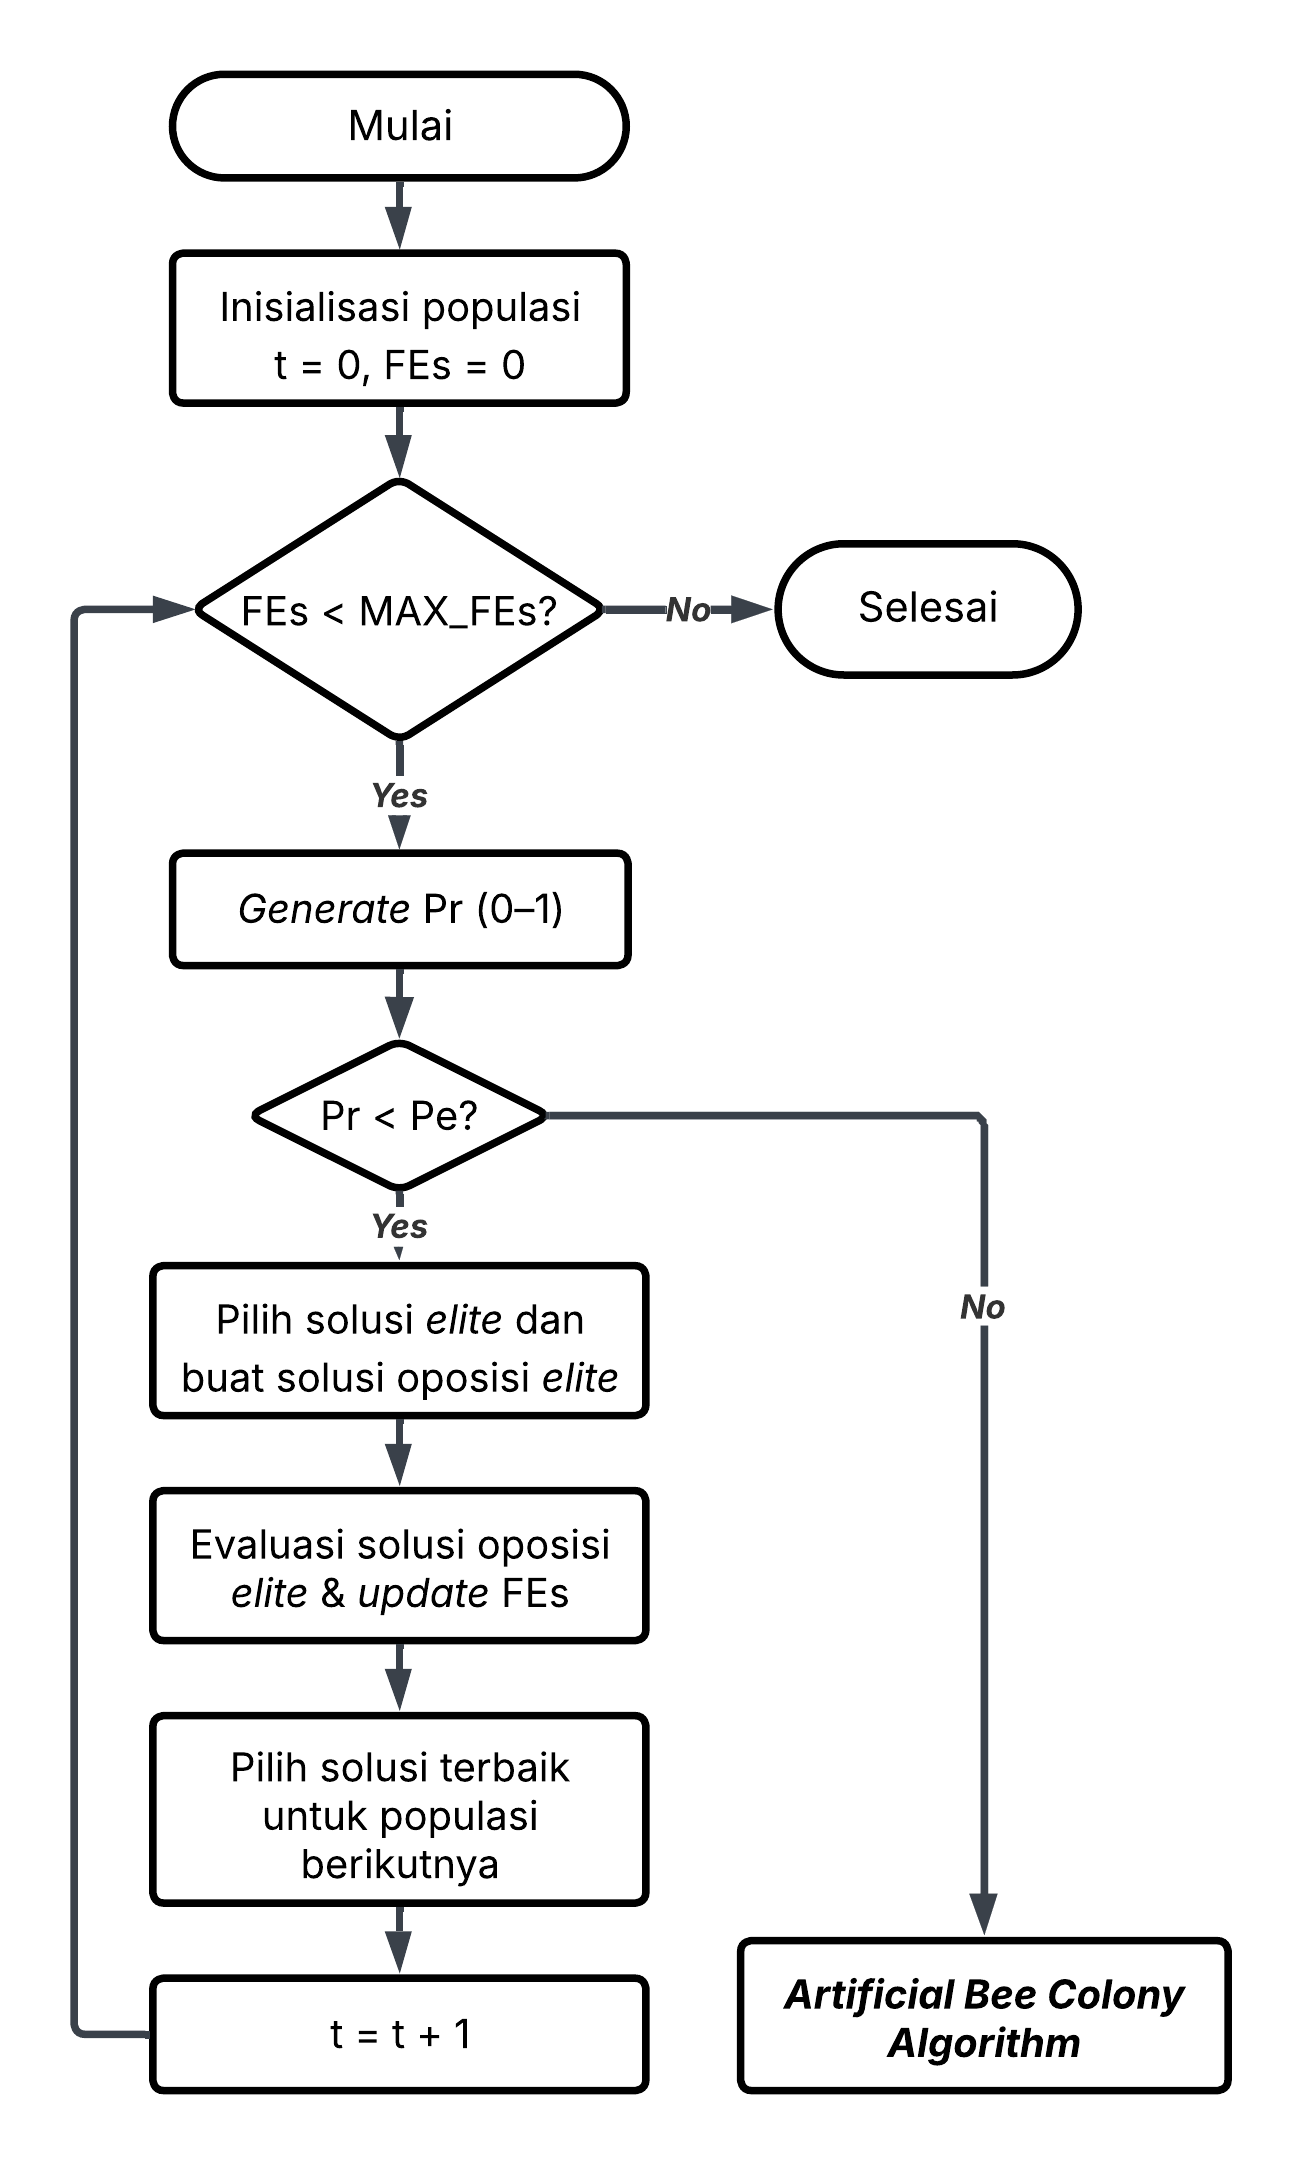
\includegraphics[width=0.85\linewidth]{gambar/Flowchart EOBL.png}
    \caption{\textit{Flowchart Elite Opposition Based Learning}}
    \label{figure:Flowchart EOBL}
\end{figure}

\subsection{Pengujian dan Evaluasi}
Pengujian dilakukan setelah implementasi untuk mengukur kinerja sistem. Pengukuran parameter yang telah ditentukan dan perbandingan dengan algoritma pembanding, seperti algoritma \textit{Swarm Intellegence}, yaitu \textit{Particle Swarm Optimization} dan algoritma \textit{metaheuristik}, yaitu \textit{Genetic Algorithm} digunakan untuk evaluasi. Dibandingkan dengan metode sebelumnya, hasil penilaian digunakan untuk memastikan sistem yang dikembangkan lebih efektif, efisien, dan ideal. Perbandingan didasarkan pada beberapa parameter sesuai dengan tabel \ref{tabel:Parameter Pengujian}.

\begin{table}[H]
    \centering
    \caption{Parameter pengujian}
    \label{tabel:Parameter Pengujian}
    \renewcommand{\arraystretch}{2.5}
    \begin{tabular}{|c|c|c|}
        \hline
        \rowcolor{blue!30}
        \textbf{No} & \textbf{Parameter} & \textbf{Rumus} \\
        \hline
        1 & \textit{Makespan} & 
        $\displaystyle \max_{i \in \text{\textit{tasks}}} \{F_i\}$ \\
        \hline
        2 & \textit{Throughput} & 
        $\displaystyle \frac{nT}{makespan}$ \\
        \hline
        3 & \textit{Average Start Time} & 
        $\displaystyle \frac{\sum_{i=1}^{n} \text{\textit{start time of} } R_i}{nR}$ \\
        \hline
        4 & \textit{Average Execution Time} & 
        $\displaystyle \frac{\sum_{i=1}^{n} \text{times } T_i}{nT}$ \\
        \hline
        5 & \textit{Average Finish Time} & 
        $\displaystyle \frac{\sum_{i=1}^{n} \text{\textit{finish time of} } R_i}{nR}$ \\
        \hline
        6 & \textit{Average Waiting Time} & 
        $\displaystyle \frac{\text{\textit{TotalDelay}}}{n}$ \\
        \hline
        7 & \textit{Imbalance Degree (\%)} & 
        $\displaystyle \frac{ET_{\max} - ET_{\min}}{ET_{\text{avg}}}$\\
        \hline
        8 & \textit{Scheduling Length} & 
        \text {\textit{scheduling time}} + \textit{makespan} \\
        \hline
        9 & \textit{Resource Utilization (\%)} & 
        $\displaystyle \frac{\sum_{i=1}^{n} \text{\textit{finish time of} } R_i}{\text{\textit{makespan}} \times nR}$ \\
        \hline
        10 & \textit{Energy Consumption} & 
        \textit{Total energy consumption} \\
        \hline
    \end{tabular}
\end{table}

\section{Bahan dan Peralatan yang digunakan}
Penelitian ini memanfaatkan berbagai perangkat lunak dan perangkat keras untuk mendukung proses simulasi, implementasi, serta analisis hasil pengujian algoritma penjadwalan tugas di lingkungan \textit{cloud computing}. Di sisi perangkat lunak, digunakan beberapa program pendukung, antara lain:
\begin{itemize} [nolistsep]
    \item \textbf{Eclipse}: digunakan sebagai \textit{Integrated Development Environment (IDE)} untuk mengembangkan kode berbasis Java.
    \item \textbf{Apache Commons Math}: \textit{library} yang berfungsi dalam komputasi matematika, termasuk analisis statistik dan optimasi.
    \item \textbf{Microsoft Excel}: digunakan untuk visualisasi data dalam bentuk grafik serta analisis hasil simulasi.
    \item \textbf{Python}: dimanfaatkan dalam pembuatan \textit{dataset stratified}.
\end{itemize}

Berikut adalah \textit{dataset} yang digunakan dalam penelitian ini:
\begin{itemize} [nolistsep]
    \item \textbf{SDSC \textit{Blue Horizon Log}}: mencakup data tugas masa lalu dari superkomputer SDSC, seperti jumlah prosesor yang digunakan, waktu mulai, dan waktu pengiriman.
    \item \textbf{\textit{Stratified Random}}: untuk memberikan distribusi pekerjaan yang lebih merata berdasarkan rentang data SDSC, kumpulan data pengambilan sampel bertingkat dikembangkan dengan menggunakan pendekatan stratifikasi.
    \item \textbf{\textit{Simple Random}}: skenario tugas umum yang disimulasikan dan dibuat dengan Excel dan memiliki antara 1.000 hingga 10.000 tugas.
\end{itemize}

Pada aspek perangkat keras untuk mendukung proses simulasi, pengembangan, dan implementasi, penelitian menggunakan perangkat keras dengan spesifikasi sebagai berikut:
\begin{itemize} [nolistsep]
    \item \textbf{Prosesor}: AMD Ryzen 5 5600U \textit{hexa-core processor}.
    \item \textbf{Memori}: RAM 16 GB.
    \item \textbf{Penyimpanan}: SSD 512 GB.
    \item \textbf{Kartu Grafis}: NVIDIA GeForce RTX 3050 (4GB GDDR6).
    \item \textbf{Sistem Operasi}: Windows 11 \textit{Home} + \textit{Office Home Student} 2021 64-bit.
\end{itemize}

Dengan pemilihan perangkat lunak dan perangkat keras yang tepat, penelitian ini menjamin bahwa proses simulasi dan implementasi berjalan lancar, menghasilkan data yang valid dan dapat diandalkan. Kombinasi alat dan bahan ini juga memungkinkan evaluasi performa algoritma penjadwalan dilakukan secara menyeluruh dan realistis, sehingga hasil penelitian dapat diaplikasikan pada kondisi nyata di lingkungan \textit{cloud computing}.

\section{Implementasi}
\subsection{Persiapan \textit{Dataset}}
Persiapan \textit{dataset} merupakan tahap awal untuk memastikan validitas dan keakuratan simulasi penjadwalan tugas. \textit{Dataset} yang dipersiapkan terdiri dari data acak yang dihasilkan secara manual melalui Microsoft Excel, \textit{dataset} log aktivitas dari SDSC, serta data hasil pengambilan sampel stratifikasi dari \textit{dataset} SDSC. Proses pembuatan dan format penyimpanan \textit{dataset} disesuaikan agar dapat digunakan secara efektif pada simulasi.

\subsubsection{\textit{Dataset Simple Random}}
\textit{Dataset Simple Random} dibuat dengan menggunakan Microsoft Excel, memanfaatkan fungsi \textit{RANDBETWEEN} untuk menghasilkan nilai acak dalam rentang antara 10.000 hingga 40.000. Fungsi ini memastikan bahwa nilai yang dihasilkan berada dalam batas yang telah ditentukan dan dilakukan secara berulang hingga mencapai jumlah baris yang diinginkan.

Proses pembuatan \textit{dataset} ini dilakukan secara bertahap, mulai dari 1.000 baris, kemudian 2.000, 3.000, hingga mencapai 10.000 baris. Setiap nilai yang dihasilkan mewakili panjang tugas (\textit{task length}) yang akan digunakan dalam simulasi penjadwalan. Setelah proses pembuatan selesai, \textit{dataset} disimpan dalam format \textit{file} teks agar dapat diintegrasikan langsung ke dalam proses simulasi penjadwalan tugas \textit{cloud}.

\begin{lstlisting} [caption={Fungsi RANDBETWEEN untuk Simple Random Dataset}, label={listing:Randbetween}, language=Java]
=RANDBETWEEN(10000, 40000)
\end{lstlisting}

Contoh fungsi yang digunakan pada Microsoft Excel terdapat pada Kode Sumber \ref{listing:Randbetween}

\begin{figure} [H]
    \centering
    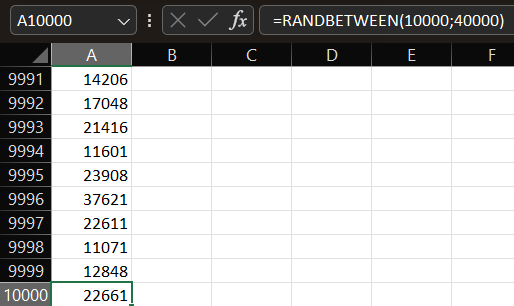
\includegraphics[width=0.5\linewidth]{gambar/Dataset Simple Random.png}
    \caption{Contoh hasil pembuatan \textit{dataset Simple Random} menggunakan Microsoft Excel}
    \label{figure:Dataset Simple Random}
\end{figure}

Gambar \ref{figure:Dataset Simple Random} menunjukkan hasil contoh pembuatan \textit{dataset Simple Random} menggunakan Microsoft Excel, yang kemudian diubah ke format teks untuk keperluan simulasi.

\subsubsection{\textit{Dataset} SDSC (\textit{The San Diego Supercomputer Center}) \textit{Blue Horizon Logs}}
\textit{Dataset} SDSC \textit{Blue Horizon Logs} merupakan \textit{dataset workload} yang berisi informasi mengenai pekerjaan atau tugas komputasi yang dijalankan pada sebuah superkomputer. \textit{Dataset} ini diambil dari laman SDSC dengan versi SDSC-BLUE-2000-4.2-cln, yang mencatat aktivitas tugas pada sistem \textit{Blue Horizon}.

Tabel \ref{tabel:SDSC} menampilkan contoh data yang diambil secara acak dari \textit{dataset} tersebut. \textit{Dataset} ini terdiri dari berbagai kolom yang merekam detail pekerjaan, seperti jumlah prosesor yang dialokasikan, waktu CPU rata-rata yang digunakan, serta berbagai atribut tambahan. Namun, \textit{dataset} asli ini mengandung banyak nilai \textit{missing} atau anomali yang ditandai dengan angka -1 pada beberapa kolomnya, yang menunjukkan ketidaklengkapan atau kehilangan data.

\begin{table} [H]
    \centering
    \small
    \caption{\textit{Dataset} SDSC \textit{Blue Horizon Logs}}
    \label{tabel:SDSC}
    \renewcommand{\arraystretch}{1.1}
    \begin{adjustbox}{max width=\textwidth}
    \begin{tabular}{rrrrrrrrrrrrrrrrrr}
    \hline
    9 & 430593 & 13 & 50866 & 256 & 25381 & -1 & 256 & 64800 & -1 & 1 & 95 & -1 & -1 & 4 & -1 & -1 & -1 \\
    10 & 430730 & 31 & 10770 & 256 & 5343 & -1 & 256 & 28800 & -1 & 1 & 95 & -1 & -1 & 4 & -1 & -1 & -1 \\
    11 & 433750 & 1878 & 12701 & 256 & 6307 & -1 & 256 & 64500 & -1 & 1 & 14 & -1 & -1 & 3 & -1 & -1 & -1 \\
    12 & 437926 & 27 & 2794 & 64 & 2601 & -1 & 64 & 60000 & -1 & 1 & 34 & -1 & -1 & 2 & -1 & -1 & -1 \\
    \multicolumn{18}{c}{\dots} \\
    250439 & 84590570 & 11 & 129758 & 32 & 93333 & -1 & 32 & 129600 & -1 & 5 & 126 & -1 & -1 & 3 & -1 & -1 & -1 \\
    250440 & 84590739 & 13 & 42 & 8 & 2.12 & -1 & 8 & 7200 & -1 & 1 & 35 & -1 & -1 & 1 & -1 & -1 & -1 \\
    \hline
    \end{tabular}
    \end{adjustbox}
\end{table}

Untuk memanfaatkan \textit{dataset} ini secara optimal dalam simulasi penjadwalan, dilakukan proses \textit{preprocessing} untuk membersihkan data dari nilai-nilai anomali tersebut. Setelah proses pembersihan, hanya dua kolom penting yang dipertahankan, yaitu \textit{allocated processors} dan \textit{average} CPU \textit{time used}.

Selanjutnya, dari dua kolom ini dilakukan perhitungan untuk memperoleh nilai \textit{task length}, yang diperoleh dengan mengalikan jumlah prosesor yang dialokasikan dengan waktu CPU rata-rata yang digunakan. Hasil pembersihan dan pengolahan ini mengurangi jumlah data dari sekitar 243.000 baris menjadi tersisa 7.395 baris yang valid untuk digunakan.

\begin{table} [H]
    \centering
    \caption{Hasil bersih \textit{dataset} SDSC}
    \label{tabel:Hasil Bersih Dataset SDSC}
    \begin{tabular}{c c c}
    \toprule
    \textit{Allocated Processors} & \textit{Average} CPU \textit{Time Used} & \textit{Task Length} \\
    \midrule
    256 & 25381   & 6497536 \\
    256 & 5343    & 1367808 \\
    256 & 6307    & 1614592 \\
    64  & 2601    & 166464 \\
    \multicolumn{1}{c}{\dots} & \multicolumn{1}{c}{\dots} & \multicolumn{1}{c}{\dots} \\
    8   & 124.38  & 995.04 \\
    8   & 0.25    & 2 \\
    \bottomrule
    \end{tabular}
\end{table}

Tabel \ref{tabel:Hasil Bersih Dataset SDSC} memperlihatkan hasil bersih \textit{dataset} SDSC setelah proses \textit{preprocessing}, yang mencakup nilai alokasi prosesor, waktu CPU yang digunakan, dan panjang \textit{task} yang akan dipakai dalam simulasi penjadwalan. Data hasil \textit{preprocessing} ini kemudian disimpan dalam format dokumen teks (.txt) untuk digunakan sebagai input pada simulasi \textit{task scheduling} di CloudSim.

\subsubsection{\textit{Stratified Random}}
\textit{Dataset Stratified Random} dibuat dengan mengamati dan menganalisis distribusi nilai dari \textit{dataset} SDSC \textit{Blue Horizon Logs}. Tahap awal dilakukan dengan menentukan nilai minimum dan maksimum dari \textit{dataset}, yang masing-masing sebesar 0,96 dan 8.783.872. Nilai ini diperoleh dengan menggunakan fungsi \textit{MIN} dan \textit{MAX} pada Microsoft Excel.

Selanjutnya, rentang data tersebut dibagi menjadi 100 kelas (\textit{strata}) dengan ukuran kelas yang sama. Cara pembagiannya, yaitu dengan membagi nilai maksimum dengan jumlah kelas, sehingga diperoleh batas atas kelas sebesar 88.000 (pembulatan dari 87.839,72). Dengan demikian, kelas pertama mencakup rentang nilai dari 0 hingga 88.000, kelas kedua dari 88.000 hingga 176.000, dan seterusnya hingga kelas ke-100 yang mencakup nilai sampai batas maksimum \textit{dataset}.

Setiap kelas memiliki batas bawah dan batas atas yang jelas, sehingga distribusi data menjadi lebih terstruktur dan representatif. Dari setiap kelas, dihitung persentase jumlah data terhadap total keseluruhan data pada \textit{dataset} SDSC. Persentase ini kemudian digunakan sebagai dasar untuk mengambil sampel data secara proporsional pada setiap kelas saat membuat \textit{dataset} baru dengan jumlah tertentu.

Misalnya, untuk membuat \textit{dataset} baru sebanyak 1.000 data, jika kelas pertama memiliki persentase 86,27\%, maka sekitar 862 data akan diambil dari rentang nilai kelas pertama tersebut. Dengan cara ini, \textit{dataset} yang dihasilkan tetap mempertahankan karakteristik distribusi asli dari data SDSC, namun dalam jumlah yang lebih kecil dan terstruktur. Data yang telah dipilah sesuai kelas ini kemudian akan disimpan dalam \textit{file} teks (.txt) secara berurutan untuk berbagai ukuran \textit{dataset}, mulai dari 1.000, 2.000, 3.000 hingga 10.000 data.

\newpage

\begin{table} [H]
    \centering
    \caption{Contoh persebaran data \textit{stratified random}}
    \renewcommand{\arraystretch}{1.2}
    \begin{tabular}{|c|c|c|c|}
    \hline
    \textbf{Kelas} & \textbf{Jumlah Data Per-kelas} & \textbf{Persentase} & \textbf{Batas Atas-Bawah} \\
    \hline
    1   & 6.380 & 86,27\% & 0 - 88.000 \\
    2   & 233   & 3,15\%  & 88.000 - 176.000 \\
    3   & 101   & 1,37\%  & 176.000 - 264.000 \\
    4   & 48    & 0,65\%  & 264.000 - 352.000 \\
    5   & 73    & 0,99\%  & 352.000 - 440.000 \\
    \multicolumn{1}{|c|}{\dots} & \multicolumn{1}{c|}{\dots} & \multicolumn{1}{c|}{\dots} &     \multicolumn{1}{c|}{\dots} \\
    100 & 1    & 0,01\%  & 8.712.000 - 8.800.000 \\
    \hline
    \end{tabular}
\end{table}

\subsection{Pembuatan \textit{Task Cloud Computing} Pada \textit{Real Environment}}
Pada \textit{real environment} pada \textit{cloud computing}, \textit{task} atau tugas yang dijalankan dapat dikategorikan berdasarkan kompleksitas pemrosesan data. Dalam penelitian ini, \textit{task} dibagi menjadi tiga jenis utama, yaitu \textit{task} ringan, sedang, dan berat. Setiap jenis \textit{task} memiliki karakteristik pemrosesan dan beban yang berbeda, yang memengaruhi cara tugas-tugas ini dikelola dan dijalankan di dalam lingkungan \textit{cloud}.

\subsubsection{A. \textit{Task} Ringan}
\textit{Task} ringan dirancang untuk memiliki beban CPU yang rendah, dengan proses yang lebih cepat dan membutuhkan waktu eksekusi yang singkat. \textit{Task} ringan dapat dilihat pada kode sumber \ref{listing:Task Ringan}

\begin{lstlisting} [caption={\textit{Task} ringan}, label={listing:Task Ringan}, language=Java]
const task = req.body.task || 'ringan';
  const db = new sqlite3.Database('./cloud_tasks.db');
  
  if (task === 'ringan') {
    const startTime = Date.now()
    db.all("SELECT name FROM products LIMIT 8000", (err, rows) => {
      if (err) return res.status(500).json({ error: err.message });

      let hashTotal = 0;
      for (let i = 0; i < 10000; i++) {
        const val = rows[0]?.name || 'default';
        hashTotal += crypto.createHash('md5').update(`light_${i}_${val}`).digest('hex').length;
      }
\end{lstlisting}

Pada \textit{task} ringan ini, program akan mengambil 8.000 nama produk dari \textit{database} dan kemudian melakukan \textit{hashing} berulang sebanyak 10.000 kali. Proses ini mensimulasikan beban CPU yang lebih rendah. Pada \textit{task} ringan, waktu eksekusi tercatat lebih cepat dibandingkan dengan \textit{task} sedang dan berat. Berdasarkan hasil dari Postman, \textit{task} ringan menunjukkan waktu eksekusi yang sangat cepat, yaitu hanya 73 ms. Proses ini dirancang untuk melakukan pemrosesan yang lebih ringan dengan beban CPU yang rendah.

\newpage

\begin{figure} [H]
    \centering
    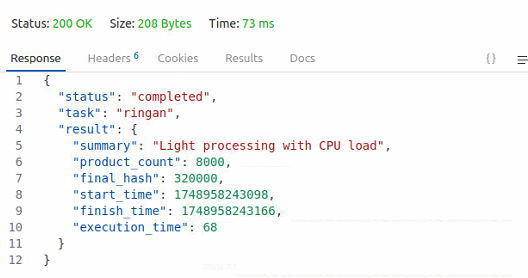
\includegraphics[width=0.75\linewidth]{gambar/Task Ringan.png}
    \caption{\textit{Task} ringan}
    \label{figure:Task Ringan}
\end{figure}

\subsubsection{B. \textit{Task} Sedang}
\textit{Task} sedang memiliki beban pemrosesan yang lebih tinggi dibandingkan dengan \textit{task} ringan. \textit{Task} sedang dapat dilihat pada kode sumber \ref{listing:Task Sedang}

\begin{lstlisting} [caption={\textit{Task} sedang}, label={listing:Task Sedang}, language=Java]
else if (task === 'sedang') {
    const startTime = Date.now()
    db.all("SELECT id FROM products LIMIT 10000", (err1, prodRows) => {
      if (err1) return res.status(500).json({ error: err1.message });
      const product_ids = prodRows.map(r => r.id);

      db.all("SELECT id FROM users LIMIT 10000", (err2, userRows) => {
        if (err2) return res.status(500).json({ error: err2.message });
        const user_ids = userRows.map(r => r.id);

        const combined_hashes = [];
        let count = 0;
        const max = 100000;

        outer:
        for (let p of product_ids) {
          for (let u of user_ids) {
            if (count >= max) break outer;
            const str = `${p}_heavy_${u}_processing`;
            const h = crypto.createHash('sha256').update(str).digest('hex');
            combined_hashes.push(h);
            count++;
          }
        }
\end{lstlisting}

Dalam \textit{task} ini, program menggabungkan ID produk dan ID pengguna untuk menghasilkan \textit{hash} SHA-256. Proses ini melibatkan pemrosesan lebih banyak data, dengan membatasi kombinasi pasangan ID produk dan pengguna hingga 100.000 pasangan. Pada \textit{task} sedang, waktu eksekusinya lebih lama dibandingkan dengan \textit{task} ringan, tetapi lebih cepat jika dibandingkan dengan \textit{task} berat. Berdasarkan hasil dari Postman, \textit{task} sedang ini menunjukkan waktu eksekusi tercatat sebesar 569 ms. \textit{Task} ini seimbang untuk pemrosesan data dengan beban CPU menengah.

\begin{figure} [H]
    \centering
    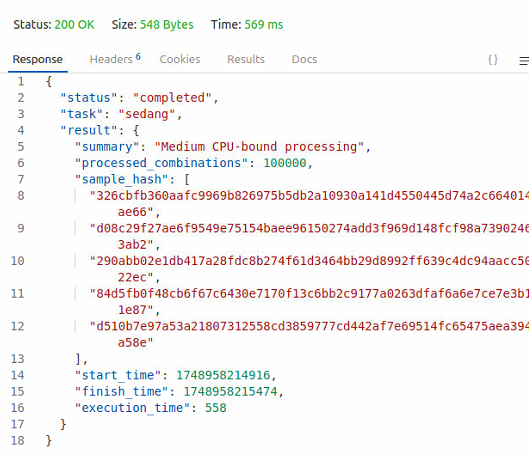
\includegraphics[width=0.75\linewidth]{gambar/Task Sedang.png}
    \caption{\textit{Task} sedang}
    \label{figure:Task Sedang}
\end{figure}

\subsubsection{C. \textit{Task} Berat}
\textit{Task} berat memiliki beban pemrosesan yang paling tinggi di antara \textit{task} ringan dan sedang. \textit{Task} berat dapat dilihat pada kode sumber \ref{listing:Task Berat}

\begin{lstlisting} [caption={\textit{Task} berat}, label={listing:Task Berat}, language=Java]
else if (task === 'berat') {
    const startTime = Date.now()
    db.all("SELECT price FROM products ORDER BY price DESC LIMIT 10000", (err, rows) => {
      if (err) return res.status(500).json({ error: err.message });

      const prices = rows.map(r => r.price);
      let total = 0;

      for (let i = 0; i < 30000; i++) {
        total += Math.floor(prices.reduce((a, b) => a + b, 0) * i % 99997);
      }
      const finishedTime = Date.now()
      const executionTime = finishedTime - startTime

      const avg = prices.reduce((a, b) => a + b, 0) / prices.length;
\end{lstlisting}

Pada \textit{task} berat ini, program akan mengurutkan harga produk secara \textit{descending} dan melakukan perhitungan matematis yang intensif untuk mensimulasikan beban yang lebih berat pada CPU dan memori. \textit{Task} berat ini memiliki waktu eksekusi yang lebih lama dibandingkan dengan \textit{task} ringan dan sedang. Berdasarkan hasil dari Postman, \textit{task} berat menunjukkan rata-rata waktu eksekusi sekitar 1.97 s, yang lebih lama daripada \textit{task} ringan dan sedang hal ini menunjukkan bahwa memerlukan waktu yang lebih lama untuk menyelesaikan pemrosesan \textit{task}. Hal ini menggambarkan bagaimana beban CPU yang lebih tinggi berdampak langsung pada durasi eksekusi dalam sistem \textit{real environment}.

\begin{figure} [H]
    \centering
    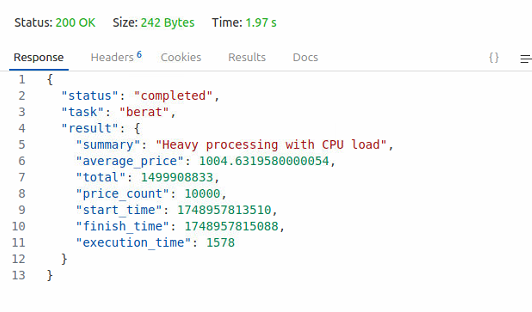
\includegraphics[width=0.75\linewidth]{gambar/Task Berat.png}
    \caption{\textit{Task} berat}
    \label{figure:Task Berat}
\end{figure}

Analisis kecepatan eksekusi setiap jenis \textit{task} (ringan, sedang, dan berat) dilakukan dengan mengulang eksekusi sebanyak 10 kali iterasi. Hasil dari percobaan ini menunjukkan rata-rata waktu eksekusi untuk setiap jenis \textit{task}, yang dapat dilihat pada tabel \ref{tabel:Execution Time Task Real Environment}. Hasil rata-rata ini memberikan gambaran yang lebih jelas mengenai perbedaan performa antara \textit{task} ringan, sedang, dan berat. \textit{Task} ringan menunjukkan waktu eksekusi tercepat, sementara \textit{task} berat membutuhkan waktu eksekusi yang lebih lama, sesuai dengan kompleksitas dan beban pemrosesan yang lebih tinggi.

\newpage

\begin{table} [H]
    \centering
    \caption{Analisis \textit{execution time} pada \textit{task real environment}}
    \label{tabel:Execution Time Task Real Environment}
    \begin{tabular}{|>{\raggedleft\arraybackslash}m{0.1\linewidth}|
                >{\raggedleft\arraybackslash}m{0.17\linewidth}|
                >{\raggedleft\arraybackslash}m{0.17\linewidth}|
                >{\raggedleft\arraybackslash}m{0.17\linewidth}|}
    \rowcolor{blue!30}
    \hline
    \multicolumn{1}{|>{\centering\arraybackslash}m{0.1\linewidth}|}{\textbf{Iterasi}} & 
    \multicolumn{1}{>{\centering\arraybackslash}m{0.17\linewidth}|}{\textbf{\textit{Task} Ringan (ms)}} & 
    \multicolumn{1}{>{\centering\arraybackslash}m{0.17\linewidth}|}{\textbf{\textit{Task} Sedang (ms)}} & 
    \multicolumn{1}{>{\centering\arraybackslash}m{0.17\linewidth}|}{\textbf{\textit{Task} Berat (ms)}} \\
    \hline
    1 & 40 & 359 & 1100 \\
    \hline
    2 & 39 & 296 & 1080 \\
    \hline
    3 & 34 & 373 & 1110 \\
    \hline
    4 & 30 & 323 & 1111 \\
    \hline
    5 & 50 & 266 & 1100 \\
    \hline
    6 & 42 & 334 & 978 \\
    \hline
    7 & 40 & 569 & 982 \\
    \hline
    8 & 48 & 320 & 1080 \\
    \hline
    9 & 73 & 372 & 1090 \\
    \hline
    10 & 33 & 326 & 1970 \\
    \hline
    \textbf{AVG} & 42,9 & 353,8 & 1160 \\
    \hline
    \end{tabular}
\end{table}

Ketiga macam \textit{task} ini kemudian akan diacak hingga mencapai total 1.000 \textit{task} yang harus dieksekusi dalam sistem. Setiap \textit{task} yang teracak akan dipresentasikan dalam format JSON yang berisi daftar tugas. Format ini memudahkan integrasi dengan API yang digunakan dalam pengelolaan dan eksekusi \textit{task} di broker. \textit{Task} dalam bentuk .json dapat dilihat pada gambar \ref{figure:Task JSON}

\begin{figure} [H]
    \centering
    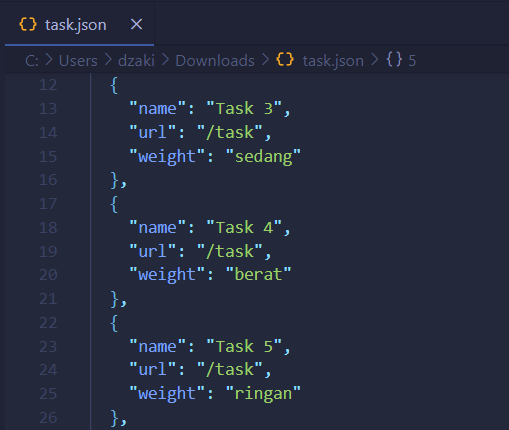
\includegraphics[width=0.5\linewidth]{gambar/Task pada Format .json.png}
    \caption{\textit{Task} pada format .json}
    \label{figure:Task JSON}
\end{figure}

Dengan menggunakan format .json, \textit{task-task} ini dapat dikirim dan diproses secara efisien dalam sistem \textit{cloud}, memanfaatkan API yang telah dikembangkan untuk mengeksekusi dan mengelola tugas-tugas tersebut di broker.

\subsection{Konfigurasi \textit{Cloud Simulator}}
\subsubsection{Pengaturan Konfigurasi pada CloudSim}
CloudSim adalah \textit{framework} simulasi \textit{cloud computing} yang memungkinkan pemodelan dan evaluasi performa algoritma penjadwalan dalam lingkungan virtualisasi. Konfigurasi awal dilakukan pada komponen utama, yaitu \textit{cloudlet} (\textit{task}), \textit{virtual machine}, dan pengaturan \textit{host} serta \textit{data center}.

\subsubsection{A. Pengaturan pada \textit{Task} atau \textit{Cloudlet} CloudSim}
Pada simulasi ini, pengaturan \textit{task} atau \textit{cloudlet} diimplementasikan melalui fungsi \textit{createCloudlet()} yang bertugas membuat dan mengonfigurasi sejumlah \textit{cloudlet} dengan parameter-parameter tertentu. Fungsi ini mengambil dua parameter yaitu ID pengguna dan jumlah \textit{cloudlet} yang akan dibuat. Implementasi pengaturan \textit{cloudlet} dapat dilihat pada kode sumber \ref{listing:createCloudlet}

\begin{lstlisting} [caption={Fungsi \textit{createCloudlet} untuk pengaturan \textit{cloudlet} CloudSim.}, label={listing:createCloudlet}, language=Java]
private static List<Cloudlet> createCloudlet(int userId, int cloudlets) {
        // Mendapatkan nilai panjang tugas dari file dataset
        ArrayList<Double> randomSeed = getSeedValue(cloudlets);

        LinkedList<Cloudlet> list = new LinkedList<Cloudlet>();

        // Parameter cloudlet
        long fileSize = 300; // Ukuran file input (byte)
        long outputSize = 300; // Ukuran file output (byte)
        int pesNumber = 1; // Jumlah CPU core yang dibutuhkan
        UtilizationModel utilizationModel = new UtilizationModelFull();

        // Membuat cloudlet dengan panjang tugas yang berbeda
        for (int i = 0; i < cloudlets; i++) {
            long length = 0;

            if (randomSeed.size() > i) {
                length = Double.valueOf(randomSeed.get(i)).longValue();
            }

            Cloudlet cloudlet = new Cloudlet(i, length, pesNumber, fileSize, outputSize, utilizationModel, utilizationModel, utilizationModel);
            cloudlet.setUserId(userId);
            list.add(cloudlet);
        }
        // Mengacak urutan cloudlet untuk simulasi yang lebih realistis
        Collections.shuffle(list);

        return list;
    }
\end{lstlisting}

Setiap \textit{cloudlet} dikonfigurasi dengan beberapa parameter penting untuk simulasi komputasi awan. Setiap \textit{cloudlet} memiliki ID yang diatur secara berurutan mulai dari 0 hingga jumlah\textit{ cloudlet}-1 dan panjang instruksi (\textit{length}) dalam \textit{Million Instructions} (MI) yang diambil dari \textit{dataset} eksternal melalui fungsi \textit{getSeedValue()}. Ukuran \textit{file} input dan \textit{output} ditetapkan masing-masing sebesar 300 byte, sementara jumlah \textit{Processing Elements} (PE) yang dibutuhkan oleh setiap \textit{cloudlet} diatur sebanyak 1 PE. Semua \textit{cloudlet} menggunakan model utilisasi penuh (\textit{UtilizationModelFull}) yang menunjukkan bahwa \textit{cloudlet} akan menggunakan seluruh sumber daya yang dialokasikan selama proses eksekusi.

Nilai \textit{length cloudlet} diambil dari tiga jenis \textit{dataset} berbeda yaitu SDSC, \textit{Random Simple}, dan \textit{Random Stratified} melalui fungsi \textit{getSeedValue()}. Penggunaan \textit{dataset} yang bervariasi ini memungkinkan evaluasi performa algoritma pada beban kerja yang berbeda-beda. Setelah semua \textit{cloudlet} dibuat, daftar \textit{cloudlet} diacak menggunakan \textit{Collections.shuffle()} untuk memastikan urutan eksekusi yang berbeda pada setiap pengujian, sehingga meningkatkan keandalan hasil simulasi.

\textit{Cloudlet} yang telah dibuat kemudian dialokasikan ke broker dengan perintah \textit{brokersubmitCloudletList(cloudletList)} pada fungsi \textit{runSimulation()}. Broker memiliki tanggung jawab untuk meneruskan \textit{cloudlet} ke \textit{virtual machine} yang sesuai berdasarkan algoritma penjadwalan yang digunakan untuk mencari solusi terbaik dalam alokasi sumber daya komputasi awan.

\subsubsection{B. Pengaturan pada \textit{Virtual Machine} CloudSim}
Fungsi \textit{createVM()} dalam simulasi ini dirancang untuk mengatur dan menginisialisasi sejumlah \textit{virtual machine} (VM) dengan berbagai spesifikasi yang akan digunakan dalam lingkungan \textit{cloud}. Implementasi fungsi ini menerima dua parameter input, yaitu ID pengguna dan jumlah VM yang akan dibuat. Kode implementasi pengaturan VM dapat dilihat pada kode sumber \ref{listing:createVM}

\begin{lstlisting} [caption={Fungsi \textit{createVM} untuk pengaturan \textit{virtual machine} CloudSim.}, label={listing:createVM}, language=Java]
private static List<Vm> createVM(int userId, int vms) {
        LinkedList<Vm> list = new LinkedList<Vm>();

        // Parameter VM
        long size = 10000; // Ukuran image (MB)
        int[] ram = { 512, 1024, 2048 }; // RAM (MB) untuk setiap jenis VM
        int[] mips = { 400, 500, 600 }; // Kecepatan processor (MIPS) untuk setiap jenis VM
        long bw = 1000; // Bandwidth (Mb/s)
        int pesNumber = 1; // Jumlah CPU core
        String vmm = "Xen"; // Virtual Machine Monitor

        Vm[] vm = new Vm[vms];

        // Membuat VM dengan karakteristik yang berbeda-beda
        for (int i = 0; i < vms; i++) {
            vm[i] = new Vm(i, userId, mips[i % 3], pesNumber, ram[i % 3], bw, size, vmm, new CloudletSchedulerSpaceShared());
            list.add(vm[i]);
        }

        return list;
    }
\end{lstlisting}

Dalam fungsi ini, setiap VM dikonfigurasi dengan spesifikasi yang bervariasi untuk mensimulasikan lingkungan komputasi awan yang heterogen. Parameter utama yang ditetapkan meliputi ukuran \textit{image} VM sebesar 10.000 MB, kapasitas RAM yang bervariasi (512, 1024, atau 2048 MB), kecepatan pemrosesan (MIPS) yang juga bervariasi (400, 500, atau 600 MIPS), \textit{bandwidth} sebesar 1000 Mbps, dan jumlah \textit{Processing Elements} (pesNumber) sebanyak 1 unit per VM. Semua VM menggunakan Xen sebagai \textit{Virtual Machine Monitor} (VMM) dan menerapkan \textit{CloudletSchedulerSpaceShared} untuk penjadwalan \textit{cloudlet}.

Fungsi ini membuat \textit{array} VM dengan ukuran sesuai parameter input lalu mengisi \textit{array} tersebut dengan VM baru yang memiliki spesifikasi berbeda. Penggunaan operator modulo (\%) pada penentuan nilai MIPS dan RAM memastikan bahwa VM akan memiliki tiga jenis spesifikasi yang berbeda yang diulang secara siklis. Hal ini berguna untuk mensimulasikan heterogenitas dalam lingkungan \textit{cloud} yang sebenarnya, di mana VM dengan spesifikasi berbeda tersedia untuk melaksanakan berbagai tugas. Setelah semua VM dibuat, daftar VM dikembalikan untuk kemudian digunakan dalam proses simulasi yang akan mengalokasikan \textit{cloudlet} ke VM yang paling optimal untuk meminimalkan waktu eksekusi dan konsumsi energi.

\subsubsection{C. Pengaturan pada \textit{Host} dan \textit{Data Center} CloudSim}
Fungsi \textit{createDatacenter()} dalam simulasi ini berperan penting untuk mengatur dan menginisialisasi \textit{data center} beserta \textit{host-host} yang ada di dalamnya. Implementasi fungsi ini menerima dua parameter, yaitu nama \textit{data center} dan ID awal untuk \textit{host}. Implementasi fungsi yang mengatur spesifikasi \textit{host} dan \textit{data center} dapat dilihat pada kode sumber \ref{createDatacenter}

\begin{lstlisting} [caption=Fungsi \textit{createDatacenter} untuk pengaturan \textit{host} dan \textit{data center} CloudSim, label={createDatacenter}, language=Java]
private static PowerDatacenter createDatacenter(String name, int hostId) {
        // Daftar host di pusat data
        List<PowerHost> hostList = new ArrayList<PowerHost>();

        // Daftar Processing Elements (PE) untuk setiap host
        List<Pe> peList1 = new ArrayList<Pe>();
        
        ... //peList2 - peList3//...

        // Kecepatan PE untuk setiap host
        int mipsunused = 300; // MIPS yang tidak digunakan
        int mips1 = 400; // MIPS untuk host 1
        int mips2 = 500; // MIPS untuk host 2
        int mips3 = 600; // MIPS untuk host 3

        // Menambahkan PE ke daftar PE untuk setiap host
        peList1.add(new Pe(0, new PeProvisionerSimple(mips1))); 
        peList1.add(new Pe(1, new PeProvisionerSimple(mips1)));
        peList1.add(new Pe(2, new PeProvisionerSimple(mips1)));
        peList1.add(new Pe(3, new PeProvisionerSimple(mipsunused)));
        
        ... //peList2 - peList3//...

        // Parameter host
        int ram = 128000; // RAM (MB)
        long storage = 1000000; // Storage (MB)
        int bw = 10000; // Bandwidth (Mb/s)
        int maxpower = 117; // Konsumsi daya maksimum
        int staticPowerPercentage = 50; // Persentase daya statis

        // Membuat host dan menambahkannya ke daftar host
        hostList.add(
            new PowerHostUtilizationHistory(
                hostId, new RamProvisionerSimple(ram),
                new BwProvisionerSimple(bw),
                storage,
                peList1,
                new VmSchedulerTimeShared(peList1),
                new PowerModelLinear(maxpower, staticPowerPercentage)));
        hostId++;
        
        ... // peList1 - peList2 // ...

        // Karakteristik pusat data
        String arch = "x86"; // Arsitektur
        String os = "Linux"; // Sistem operasi
        String vmm = "Xen"; // Virtual Machine Monitor
        double time_zone = 10.0; // Zona waktu
        double cost = 3.0; // Biaya penggunaan per jam
        double costPerMem = 0.05; // Biaya per GB RAM
        double costPerStorage = 0.1; // Biaya per GB storage
        double costPerBw = 0.1; // Biaya per Gb/s bandwidth
        LinkedList<Storage> storageList = new LinkedList<Storage>();

        // Membuat karakteristik pusat data
        DatacenterCharacteristics characteristics = new DatacenterCharacteristics(
            arch, os, vmm, hostList, time_zone, cost, costPerMem, costPerStorage, costPerBw);

        // Membuat pusat data
        PowerDatacenter datacenter = null;
        try {
            datacenter = new PowerDatacenter(name, characteristics, new PowerVmAllocationPolicySimple(hostList), storageList, 9); 
        } catch (Exception e) {
            e.printStackTrace();
        }

        return datacenter;
    }
\end{lstlisting}

Dalam fungsi ini terdapat dua bagian utama, yaitu konfigurasi \textit{host} dan konfigurasi \textit{data center}. Untuk konfigurasi \textit{host}, fungsi ini membuat tiga jenis \textit{host} dengan spesifikasi yang berbeda. Setiap \textit{host} dilengkapi dengan \textit{Processing Elements} (PE) dengan kecepatan pemrosesan yang bervariasi (400, 500, dan 600 MIPS). Setiap \textit{host} memiliki empat PE, dengan tiga PE aktif dan satu PE cadangan dengan kecepatan 300 MIPS. Selain itu, setiap \textit{host} dikonfigurasi dengan kapasitas RAM sebesar 128.000 MB, penyimpanan sebesar 1.000.000 MB, dan \textit{bandwidth} sebesar 10.000 Mbps.

\textit{Host-host} ini juga menggunakan model daya linear dengan daya maksimum 117 Watt dan persentase daya statis sebesar 50\%. Penggunaan model daya ini penting untuk mensimulasikan konsumsi energi dalam lingkungan \textit{cloud computing}, yang menjadi salah satu metrik evaluasi performa algoritma penjadwalan. Semua \textit{host} menggunakan aturan \textit{VmSchedulerTimeShared} untuk alokasi waktu prosesor di antara VM yang berjalan.

Untuk konfigurasi \textit{data center}, fungsi ini menetapkan karakteristik seperti arsitektur "x86", sistem operasi "Linux", VMM "Xen", dan berbagai parameter biaya operasional (\textit{cost} per CPU, \textit{memory}, \textit{storage}, dan \textit{bandwidth}). \textit{Data center} menggunakan aturan \textit{PowerVmAllocationPolicySimple} untuk alokasi VM ke \textit{host}.

Dalam simulasi ini, enam \textit{data center} identik dibuat dengan tiga \textit{host} per \textit{data center}. Pendekatan ini memungkinkan evaluasi performa algoritma penjadwalan dalam lingkungan \textit{cloud} yang terdistribusi dan heterogen, menyerupai infrastruktur \textit{cloud} di dunia nyata. Pengukuran konsumsi energi dari seluruh \textit{data center} kemudian digunakan sebagai salah satu metrik utama untuk mengevaluasi efisiensi algoritma penjadwalan tersebut.

\subsubsection{Pengaturan Parameter Penilaian pada CloudSim}
Konfigurasi parameter penilaian dilakukan untuk mengevaluasi performa algoritma dalam simulasi penjadwalan tugas. Pengaturan parameter penilaian ini disesuaikan dengan konfigurasi parameter pengujian yang telah ditentukan sebelumnya.

\subsubsection{A. \textit{Makespan} pada CloudSim}
\textit{Makespan} merupakan parameter yang mengukur waktu total yang diperlukan untuk menyelesaikan seluruh tugas dalam simulasi. Parameter ini diimplementasikan dengan menginisialisasi variabel \textit{makespan} bernilai 0.0, yang kemudian diperbarui dengan waktu selesai (\textit{finish time}) dari \textit{cloudlet} terakhir yang dieksekusi.

Perhitungan ini dilakukan dengan mengakses properti \textit{getFinishTime()} dari \textit{cloudlet} terakhir, yang memberikan waktu penyelesaian paling akhir dari seluruh tugas.

\begin{lstlisting} [caption={Fungsi perhitungan \textit{makespan} CloudSim}, language=Java]
// Inisialisasi makespan
double makespan = 0.0;

// Perhitungan makespan total dengan menambahkan finish time cloudlet terakhir
double makespan_total = makespan + cloudlet.getFinishTime();

// Menampilkan hasil makespan
System.out.println(String.format("Makespan: %,f", makespan_total));
\end{lstlisting}

\subsubsection{B. \textit{Average Start Time} pada CloudSim}
\textit{Average start time} merupakan parameter yang mengukur rata-rata waktu dimulainya eksekusi setiap \textit{cloudlet} dalam simulasi. Parameter ini menunjukkan kecepatan sistem dalam memulai proses tugas dan dihitung dengan menjumlahkan waktu mulai seluruh \textit{cloudlet}, kemudian membaginya dengan jumlah total \textit{cloudlet}. Implementasinya dimulai dengan menginisialisasi variabel \textit{totalStartTime} bernilai 0.0, dilanjutkan dengan iterasi melalui setiap \textit{cloudlet} untuk mengumpulkan waktu mulai menggunakan metode \textit{getExecStartTime()}.

\begin{lstlisting} [caption={Fungsi perhitungan \textit{average start time} CloudSim}, language=Java]
// Inisialisasi total waktu mulai
double totalStartTime = 0.0;

// Menghitung total waktu mulai dari semua cloudlet
for (int i = 0; i < size; i++) {
    totalStartTime += cloudletList.get(i).getExecStartTime();
}

// Menghitung rata-rata waktu mulai
double avgStartTime = totalStartTime / size;

// Menampilkan hasil average start time
System.out.println(String.format("Average StartTime: %,6f", avgStartTime));
\end{lstlisting}

\subsubsection{C. \textit{Average Finish Time} pada CloudSim}
\textit{Average finish time} mengukur rata-rata waktu yang diperlukan untuk menyelesaikan seluruh \textit{cloudlet} dalam simulasi. Parameter ini menunjukkan efisiensi sistem dalam menuntaskan beban kerja komputasi dan dihitung dengan menjumlahkan waktu selesai seluruh \textit{cloudlet}, lalu membaginya dengan jumlah total \textit{cloudlet}. Implementasinya dimulai dengan menginisialisasi variabel \textit{totalTime} bernilai 0.0, dilanjutkan dengan iterasi untuk mengumpulkan waktu selesai setiap \textit{cloudlet} menggunakan \textit{getFinishTime()}. 

\begin{lstlisting} [caption={Fungsi perhitungan \textit{average finish time} CloudSim}, language=Java]
// Inisialisasi total waktu selesai
double totalTime = 0.0;

// Menghitung total waktu selesai dari semua cloudlet
for (int i = 0; i < size; i++) {
    totalTime += cloudletList.get(i).getFinishTime();
}

// Menghitung rata-rata waktu selesai
double avgTAT = totalTime / size;

// Menampilkan hasil average finish time
System.out.println(String.format("Average FinishTime: %,6f", avgTAT));
\end{lstlisting}

\textit{Average finish time} mengindikasikan kecepatan sistem dalam menyelesaikan tugas, efisiensi pengelolaan sumber daya, dan kemampuan menangani beban kerja.

\subsubsection{D. \textit{Average Execution Time} pada CloudSim}
\textit{Average execution time} mengukur rata-rata waktu yang diperlukan untuk menjalankan setiap \textit{cloudlet} dalam simulasi. Parameter ini menunjukkan efisiensi sistem dalam memproses beban kerja komputasi dan dihitung dengan menjumlahkan waktu eksekusi aktual seluruh \textit{cloudlet}, kemudian membaginya dengan jumlah total \textit{cloudlet}. Implementasinya dimulai dengan menginisialisasi variabel \textit{ExecTime} bernilai 0.0, dilanjutkan dengan iterasi untuk mengumpulkan waktu eksekusi setiap \textit{cloudlet} menggunakan \textit{getActualCPUTime()}. 

\begin{lstlisting} [caption={Fungsi perhitungan \textit{average execution time} CloudSim}, language=Java]
// Inisialisasi total waktu eksekusi
double ExecTime = 0.0;

// Menghitung total waktu eksekusi dari semua cloudlet
for (int i = 0; i < size; i++) {
    ExecTime += cloudletList.get(i).getActualCPUTime();
}

// Menghitung rata-rata waktu eksekusi
double avgExecTime = ExecTime / size;

// Menampilkan hasil average execution time
System.out.println(String.format("Average Execution Time: %,6f", avgExecTime));
\end{lstlisting}

\textit{Average execution time} menggambarkan efisiensi penggunaan sumber daya CPU, mengindikasikan kecepatan pemrosesan tugas, dan membantu evaluasi kemampuan sistem dalam menangani beban kerja komputasi.

\subsubsection{E. \textit{Average Waiting Time} pada CloudSim}
\textit{Average waiting time} mengukur rata-rata waktu yang dihabiskan \textit{cloudlet} dalam antrian sebelum diproses. Parameter ini menggambarkan efisiensi sistem dalam mengelola antrian tugas dan responsivitas terhadap permintaan eksekusi baru. Perhitungannya sederhana, yaitu dengan mengambil waktu tunggu dari \textit{cloudlet} terakhir menggunakan \textit{getWaitingTime()}, kemudian membaginya dengan jumlah total \textit{cloudlet}. 

\begin{lstlisting} [caption={Fungsi perhitungan \textit{average waiting time} CloudSim}, language=Java]
// Menghitung rata-rata waktu tunggu
double avgWT = cloudlet.getWaitingTime() / size;

// Menampilkan hasil average waiting time
System.out.println(String.format("Average Waiting time: %,6f", avgWT));
\end{lstlisting}

\textit{Average waiting time} mengindikasikan kemampuan sistem mengelola antrian, mengidentifikasi \textit{bottleneck} dalam proses penjadwalan, dan menunjukkan kecepatan respons terhadap tugas baru.

\subsubsection{F. \textit{Scheduling Length} pada CloudSim}
\textit{Scheduling length} mengukur total waktu yang diperlukan untuk menjadwalkan dan menjalankan seluruh tugas dalam simulasi. Parameter ini memberikan gambaran komprehensif tentang efisiensi sistem dengan mempertimbangkan keseluruhan proses dari waktu tunggu hingga eksekusi. Perhitungannya sederhana yaitu menjumlahkan total waktu tunggu (\textit{waitTimeSum}) dan total \textit{makespan} (\textit{makespan\_total}). Implementasinya melibatkan akumulasi waktu tunggu dari setiap \textit{cloudlet} menggunakan \textit{getWaitingTime()}, kemudian menambahkannya dengan total \textit{makespan}. 

\begin{lstlisting} [caption={Fungsi perhitungan \textit{scheduling length} CloudSim}, language=Java]
// Menghitung scheduling length
double scheduling_length = waitTimeSum + makespan_total;

// Menampilkan hasil scheduling length
Log.printLine(String.format("Scheduling Length: %,f", scheduling_length));
\end{lstlisting}

\textit{Scheduling length} menunjukkan efisiensi keseluruhan proses penjadwalan, mengidentifikasi waktu total penyelesaian beban kerja, dan mengevaluasi kemampuan sistem dalam mengoptimalkan alokasi sumber daya.

\subsubsection{G. \textit{Throughput} pada CloudSim}
\textit{Throughput} mengukur jumlah \textit{cloudlet} yang berhasil diselesaikan per satuan waktu, menggambarkan produktivitas sistem dalam menyelesaikan tugas komputasi. Perhitungannya dilakukan dengan membagi jumlah total \textit{cloudlet} dengan waktu selesai maksimum (\textit{maxFT}) dari seluruh \textit{cloudlet}. Implementasinya melibatkan pencarian waktu selesai terpanjang melalui iterasi setiap \textit{cloudlet}, membandingkan nilai \textit{getFinishTime()} dengan \textit{maxFT}, kemudian membagi jumlah \textit{cloudlet} dengan nilai \textit{maxFT} tertinggi.

\begin{lstlisting} [caption={Fungsi perhitungan \textit{throughput} CloudSim}, language=Java]
// Inisialisasi waktu selesai maksimum
double maxFT = 0.0;

// Mencari waktu selesai maksimum di antara semua cloudlet
for (int i = 0; i < size; i++) {
    double currentFT = cloudletList.get(i).getFinishTime();
    if (currentFT > maxFT) {
        maxFT = currentFT;
    }
}

// Menghitung throughput
double throughput = size / maxFT;

// Menampilkan hasil throughput
System.out.println(String.format("Throughput: %,9f", throughput));
\end{lstlisting}

\textit{Throughput} mengindikasikan tingkat produktivitas sistem, efisiensi pemrosesan beban kinerja, dan kapasitas penanganan jumlah tugas per satuan waktu.

\subsubsection{H. \textit{Resource Utilization} pada CloudSim}
\textit{Resource utilization} mengukur efisiensi penggunaan sumber daya komputasi dalam simulasi. Parameter ini menunjukkan seberapa optimal sistem memanfaatkan sumber daya yang tersedia dan dihitung dengan membagi total waktu CPU (\textit{CPUTimeSum}) dengan hasil kali antara \textit{makespan} dan jumlah VM (54), kemudian dikonversi menjadi persentase. Implementasinya melibatkan akumulasi waktu CPU dari setiap \textit{cloudlet} menggunakan \textit{getActualCPUTime()}, pembagian dengan nilai \textit{makespan\_total} dikalikan jumlah VM, dan pengkonversian ke persentase. 

\begin{lstlisting} [caption={Fungsi perhitungan \textit{resource utilization} CloudSim}, language=Java]
// Menghitung resource utilization
double resource_utilization = (CPUTimeSum / (makespan_total * 54)) * 100;

// Menampilkan hasil resource utilization
Log.printLine(String.format("Resouce Utilization: %,f", resource_utilization));
\end{lstlisting}

\textit{Resource utilization} mengindikasikan efisiensi pemanfaatan sumber daya, membantu identifikasi \textit{underutilization} atau \textit{overutilization}, dan menunjukkan keseimbangan beban kerja antar VM.

\subsubsection{I. \textit{Energy Consumption} pada CloudSim}
\textit{Energy consumption} mengukur total energi yang digunakan oleh sistem selama simulasi. Parameter ini menggambarkan efisiensi energi dalam menjalankan dan menyelesaikan tugas komputasi, dihitung dengan menjumlahkan daya dari semua \textit{data center} dan mengkonversinya ke \textit{kilowatt-hour} (kWh). Implementasinya melibatkan akumulasi daya dari masing-masing \textit{data center} menggunakan \textit{getPower()}, kemudian mengkonversinya dari \textit{watt-second} ke kWh dengan membagi hasil penjumlahan dengan 3600 (detik dalam satu jam) dan 1000 (watt ke kilowatt). 

\begin{lstlisting} [caption={Fungsi Perhitungan \textit{energy consumption} CloudSim}, language=Java]
// Menghitung total energy consumption
double totalEnergy = (datacenter1.getPower() + datacenter2.getPower() + datacenter3.getPower() + 
                    datacenter4.getPower() + datacenter5.getPower() + datacenter6.getPower()) / (3600 * 1000);

// Menampilkan hasil energy consumption
Log.printLine(String.format("Total Energy Consumption: %,2f kWh", totalEnergy));
\end{lstlisting}

Energy consumption mengindikasikan efisiensi energi sistem, membantu identifikasi pemborosan daya, dan menunjukkan dampak lingkungan dari operasi \textit{cloud computing}.

\subsubsection{J. \textit{Imbalance Degree} pada CloudSim}
\textit{Imbalance degree} mengukur tingkat ketidakmerataan beban kerja antara waktu eksekusi tertinggi dan terendah pada prosesor. Parameter ini menunjukkan keseimbangan distribusi tugas antar VM dalam sistem dan dihitung dengan membagi selisih antara nilai maksimum dan minimum waktu eksekusi dengan rata-rata waktu CPU. Implementasinya memanfaatkan \textit{DoubleSummaryStatistics} dari \textit{array response\_time} untuk mendapatkan nilai maksimum dan minimum secara efisien, kemudian membagi selisihnya dengan rata-rata waktu CPU (\textit{CPUTimeSum/totalValues}). 

\begin{lstlisting} [caption={Fungsi perhitungan \textit{imbalance degree} CloudSim}, language=Java]
// Mendapatkan statistik dari response_time
DoubleSummaryStatistics stats = DoubleStream.of(response_time).summaryStatistics();

// Menghitung imbalance degree
double degree_of_imbalance = (stats.getMax() - stats.getMin()) / (CPUTimeSum / totalValues);

// Menampilkan hasil imbalance degree
System.out.println(String.format("Imbalance Degree: %,3f", degree_of_imbalance));
\end{lstlisting}

\textit{Imbalance degree} mengindikasikan keseimbangan distribusi beban kerja, membantu identifikasi \textit{bottleneck} akibat ketidakseimbangan, dan mengevaluasi efektivitas algoritma dalam menyeimbangkan beban antar VM.

\subsection{Konfigurasi Implementasi \textit{Real Environment}}
Implementasi lingkungan nyata untuk pengujian algoritma ABC dilakukan menggunakan kombinasi VirtualBox sebagai \textit{host} dan Docker untuk virtualisasi \textit{container}. Pendekatan ini dipilih untuk mensimulasikan lingkungan \textit{cloud computing} yang lebih realistis dengan kemampuan kontrol sumber daya yang lebih baik dan terukur.

\subsubsection{Konfigurasi \textit{Container Virtual Machine} pada \textit{Real Environment}}
Konfigurasi \textit{container} Docker diatur menggunakan Dockerfile yang menggunakan Node.js versi 18 sebagai \textit{base image}. Dockerfile mendefinisikan langkah-langkah pembuatan \textit{container}, instalasi dependensi dari \textit{package.json}, hingga penyalinan kode aplikasi dan perintah untuk menjalankan aplikasi. Struktur ini memastikan konsistensi \textit{environment} untuk setiap \textit{instance} aplikasi yang dijalankan.

\begin{lstlisting} [caption={Dockerfile}, language=Java]
FROM node:18
WORKDIR /app
COPY package*.json ./
RUN npm install
COPY . .
CMD ["node", "index.js"]
\end{lstlisting}

\textit{Container} dikelola menggunakan \textit{docker-compose.yml} yang mendefinisikan dua \textit{service} utama: vm1 dan vm2. Kedua \textit{service} ini memiliki spesifikasi \textit{resource} yang berbeda untuk mensimulasikan heterogenitas dalam lingkungan \textit{cloud}. VM1 dikonfigurasi dengan 1 CPU \textit{core} dan 512MB RAM, sementara VM2 memiliki 1 CPU \textit{core} dengan 1024MB RAM. Setiap \textit{container} memiliki \textit{port mapping} yang berbeda (31001 dan 31002) yang diarahkan ke port 3000 \textit{internal container}, memungkinkan akses dari luar \textit{container}.

\begin{lstlisting} [caption={docker-compose.yml}, language=Java]
services:
       vm1:
         build:
           context: ./app
           dockerfile: Dockerfile
         container_name: vm1
         ports:
           - "31001:3000"
         deploy:
           resources:
             limits:
               cpus: '1'
               memory: 512m
         networks:
           - ts-network
  vm2:
    # Konfigurasi serupa dengan spesifikasi berbeda
    memory: 1024m
    # ...
\end{lstlisting}

\subsubsection{Konfigurasi \textit{Host} dan Broker pada \textit{Real Environment}}
Pada implementasi sistem ini, konfigurasi \textit{host} dan broker dilakukan menggunakan VirtualBox dengan sistem operasi Ubuntu. Setiap \textit{host} dan broker memiliki spesifikasi perangkat keras yang mendukung tugas komputasi awan secara efisien, yaitu CPU 4 \textit{core} dan RAM 4 GB. Broker berperan sebagai entitas utama dalam mengelola penjadwalan tugas (\textit{task scheduling}) dan mengatur interaksi antar komponen sistem yang mengkoordinasikan alokasi sumber daya ke mesin virtual. Broker dikonfigurasi dengan spesifikasi lebih tinggi, yaitu CPU 8 \textit{core} dan RAM 8 GB. Detail lebih lanjut mengenai spesifikasi \textit{host} dan broker dapat dilihat pada gambar \ref{figure:Spesifikasi Host pada Real Environment} dan gambar \ref{figure:Spesifikasi Broker Environment}.

\newpage

\begin{figure} [H]
    \centering
    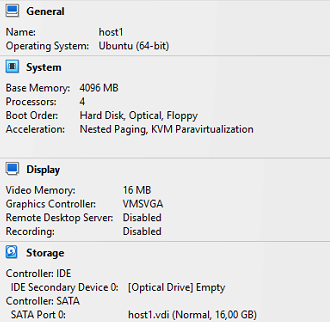
\includegraphics[width=0.5\linewidth]{gambar/Spesifikasi Host pada Real Environment.png}
    \caption{Spesifikasi \textit{host} pada \textit{real environment}}
    \label{figure:Spesifikasi Host pada Real Environment}
\end{figure}

\begin{figure} [H]
    \centering
    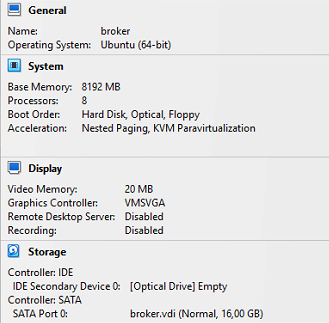
\includegraphics[width=0.5\linewidth]{gambar/Spesifikasi Broker.png}
    \caption{Spesifikasi \textit{broker} pada \textit{real environment}}
    \label{figure:Spesifikasi Broker Environment}
\end{figure}

\subsubsection{Pengaturan Parameter Penilaian pada \textit{Real Environment}}
\subsubsection{A. \textit{Makespan} pada \textit{Real Environment}}
\textit{Makespan} merupakan parameter penilaian yang mengukur total waktu yang dibutuhkan untuk menyelesaikan seluruh \textit{task} dalam sistem \textit{cloud}. Dalam implementasinya, perhitungan \textit{makespan} dilakukan dengan mencatat dua \textit{timestamp} utama menggunakan fungsi \textit{Date.now():} \textit{timestamp} awal (\textit{makespanStart}) yang direkam saat \textit{task} pertama mulai diproses, dan \textit{timestamp} akhir (\textit{makespanEnd}) yang direkam saat task terakhir selesai dieksekusi. Perhitungan \textit{makespan} dilakukan dengan mengurangi \textit{makespanEnd} dengan \textit{makespanStart} untuk mendapatkan total durasi dalam milidetik, yang kemudian dikonversi ke dalam satuan detik dengan membagi hasil tersebut dengan 1000.

\begin{lstlisting} [caption={Fungsi perhitungan \textit{makespan} pada \textit{real environment}}, language=Java]
// Mencatat waktu mulai saat task pertama diproses
if (!makespanStart) makespanStart = Date.now();

// Setelah semua task selesai, hitung makespan
if (completedTasks === totalTasks) {
  makespanEnd = Date.now();
  const makespanDurationSec = (makespanEnd - makespanStart) / 1000;
}
\end{lstlisting}

\subsubsection{B. \textit{Average Start Time} pada \textit{Real Environment}}
\textit{Average start time} merupakan parameter yang mengukur rata-rata waktu dimulainya eksekusi setiap \textit{task} dalam sistem \textit{cloud}. Implementasinya dilakukan dengan mengumpulkan waktu mulai (\textit{start time}) dari setiap \textit{task} ke dalam \textit{array startTimes}, di mana waktu yang dicatat adalah relatif terhadap waktu mulai \textit{makespan}. Perhitungan \textit{average start time} dilakukan dengan menjumlahkan seluruh waktu mulai menggunakan fungsi \textit{reduce()}, kemudian membagi total tersebut dengan jumlah \textit{task} yang telah dieksekusi (\textit{startTimes.length}).

\begin{lstlisting} [caption={Fungsi perhitungan \textit{average start time} pada \textit{real environment}}, language=Java]
// Mencatat waktu mulai relatif
const relativeStartTime = startTime - makespanStart;
startTimes.push(relativeStartTime);

// Setelah semua task selesai, hitung average start time
if (completedTasks === totalTasks) {
  const avgStart = startTimes.reduce((a, b) => a + b, 0) / startTimes.length;
  ...
}
\end{lstlisting}

\subsubsection{C. \textit{Average Finish Time} pada \textit{Real Environment}}
\textit{Average finish time} merupakan parameter yang mengukur rata-rata waktu penyelesaian seluruh \textit{task} dalam sistem \textit{cloud}. Implementasinya dilakukan dengan mencatat waktu selesai (\textit{finish time}) setiap \textit{task} yang berhasil dieksekusi ke dalam \textit{array finishTimes}, di mana waktu yang disimpan adalah relatif terhadap waktu mulai \textit{makespan}. Setiap kali sebuah \textit{task} selesai dieksekusi, sistem menyimpan \textit{timestamp} penyelesaiannya. Perhitungan \textit{average finish time} dilakukan dengan menjumlahkan seluruh waktu penyelesaian menggunakan fungsi \textit{reduce()}, kemudian membagi total tersebut dengan jumlah keseluruhan \textit{task} yang telah selesai dieksekusi (\textit{finishTimes.length}).

\begin{lstlisting} [caption={Fungsi perhitungan \textit{average finish time} pada \textit{real environment}}, language=Java]
// Mencatat waktu selesai relatif
const relativeFinishTime = finishTime - makespanStart;
finishTimes.push(relativeFinishTime);

// Setelah semua task selesai, hitung average finish time
if (completedTasks === totalTasks) {
  const avgFinish = finishTimes.reduce((a, b) => a + b, 0) / finishTimes.length;
  ...
}
\end{lstlisting}

\subsubsection{D. \textit{Average Execution Time} pada \textit{Real Environment}}
\textit{Average execution time} merupakan parameter yang mengukur rata-rata waktu yang dibutuhkan untuk mengeksekusi setiap \textit{task} dalam sistem \textit{cloud}. Implementasinya dilakukan dengan mencatat durasi eksekusi (\textit{execution time}) setiap \textit{task} yang diproses ke dalam \textit{array executionTimes}. Waktu eksekusi ini diperoleh langsung dari \textit{response worker} setelah menyelesaikan \textit{task} dan merepresentasikan durasi aktual yang dibutuhkan \textit{worker} untuk memproses sebuah \textit{task}. Perhitungan \textit{average execution time} dilakukan dengan menjumlahkan seluruh waktu eksekusi menggunakan fungsi \textit{reduce()}, kemudian membagi total tersebut dengan jumlah \textit{task} yang telah dieksekusi (\textit{executionTimes.length}).

\begin{lstlisting} [caption={Fungsi perhitungan \textit{average execution time} pada \textit{real environment}}, language=Java]
// Mendapatkan execution time dari response worker
const execTime = response.data?.result?.execution_time || 0;
executionTimes.push(execTime);

// Setelah semua task selesai, hitung average execution time
if (completedTasks === totalTasks) {
  const avgExec = executionTimes.reduce((a, b) => a + b, 0) / executionTimes.length;
  ...
}
\end{lstlisting}

\subsubsection{E. \textit{Average Waiting Time} pada \textit{Real Environment}}
\textit{Average waiting time} merupakan parameter yang mengukur rata-rata waktu tunggu setiap \textit{task} sebelum dieksekusi dalam sistem \textit{cloud}. Implementasinya dilakukan dengan menghitung waktu tunggu, di mana \textit{task} pertama memiliki waktu tunggu 0, sementara \textit{task-task} berikutnya memiliki waktu tunggu berdasarkan waktu penyelesaian relatif \textit{task} sebelumnya. Setiap waktu tunggu disimpan dalam \textit{array waitingTimes}. Perhitungan \textit{average waiting time} dilakukan dengan menjumlahkan seluruh waktu tunggu menggunakan fungsi \textit{reduce()} dan membaginya dengan total jumlah \textit{task} (\textit{totalTasks}).

\begin{lstlisting} [caption={Fungsi perhitungan \textit{average waiting time} pada \textit{real environment}}, language=Java]
// Implementasi waiting time sesuai jurnal
let waitingTime;
if (completedTasks === 0) {
  waitingTime = 0;
} else {
  waitingTime = lastFinishTime; // Waktu tunggu relatif terhadap awal simulasi
}
waitingTimes.push(waitingTime);

// Update waktu penyelesaian terakhir (untuk waktu tunggu task berikutnya)
lastFinishTime = relativeFinishTime;

// Setelah semua task selesai, hitung average waiting time
if (completedTasks === totalTasks) {
  const totalWaitingTime = waitingTimes.reduce((a, b) => a + b, 0);
  const avgWaitingTime = totalWaitingTime / totalTasks;
  ...
}
\end{lstlisting}

\subsubsection{F. \textit{Scheduling Length} pada \textit{Real Environment}}
\textit{Scheduling length} merupakan parameter penilaian yang mengukur total waktu penyelesaian keseluruhan proses penjadwalan \textit{task}, termasuk waktu tunggu. Dalam implementasinya, perhitungan \textit{scheduling length} dilakukan dengan menjumlahkan total waktu tunggu (\textit{totalWaitingTime}) dengan total durasi pelaksanaan (\textit{makespan} dalam milidetik). Berbeda dengan \textit{makespan} yang hanya mengukur waktu dari \textit{task} pertama dimulai hingga \textit{task} terakhir selesai, \textit{scheduling length} mencakup keseluruhan waktu dari perspektif sistem termasuk waktu tunggu kumulatif semua \textit{task}. 

\begin{lstlisting} [caption={Fungsi perhitungan \textit{scheduling length} pada \textit{real environment}}, language=Java]
if (completedTasks === totalTasks) {
  // Menghitung total waktu tunggu
  const totalWaitingTime = waitingTimes.reduce((a, b) => a + b, 0);
  
  // Menghitung scheduling length
  const schedulingLength = totalWaitingTime + (makespanEnd - makespanStart);
  ...
}
\end{lstlisting}

\subsubsection{G. \textit{Throughput} pada \textit{Real Environment}}
\textit{Throughput} merupakan parameter yang mengukur jumlah \textit{task} yang berhasil diselesaikan per satuan waktu dalam sistem \textit{cloud}. Implementasinya dilakukan dengan membagi total jumlah \textit{task} (\textit{totalTasks}) dengan durasi \textit{makespan} dalam satuan detik (\textit{makespanDurationSec}). Durasi \textit{makespan} dihitung dengan mengurangi waktu akhir (\textit{makespanEnd}) dengan waktu awal (\textit{makespanStart}) dan dikonversi ke dalam satuan detik.

\begin{lstlisting} [caption={Fungsi perhitungan \textit{throughput} pada \textit{real environment}}, language=Java]
if (completedTasks === totalTasks) {
  makespanEnd = Date.now();
  const makespanDurationSec = (makespanEnd - makespanStart) / 1000;
  const throughput = totalTasks / makespanDurationSec;
  ...
}
\end{lstlisting}

\subsubsection{H. \textit{Resource Utilization} pada \textit{Real Environment}}
\textit{Resource utilization} merupakan parameter yang mengukur tingkat pemanfaatan sumber daya CPU pada sistem \textit{cloud}. Implementasinya dilakukan dengan mengumpulkan data penggunaan CPU dari setiap \textit{worker} melalui \textit{endpoint '/cpu-usage-report'} yang menerima laporan penggunaan CPU secara \textit{real-time}. Setiap \textit{worker} mengirimkan data berupa \textit{host} (identifikasi \textit{worker}) dan nilai rata-rata penggunaan CPU (\textit{avgCpu}) yang disimpan dalam \textit{array cpuUsages}. Perhitungan \textit{resource utilization} dilakukan dengan mengelompokkan data penggunaan CPU berdasarkan \textit{host} menggunakan objek \textit{grouped}, menghitung rata-rata penggunaan CPU untuk setiap \textit{host}, kemudian menghitung rata-rata keseluruhan dari semua \textit{host}.

\begin{lstlisting} [caption={Fungsi perhitungan \textit{resource utilization} pada \textit{real environment}}, language=Java]
// Endpoint untuk menerima laporan penggunaan CPU
app.post('/cpu-usage-report', (req, res) => {
  const { host, avgCpu } = req.body;
  cpuUsages.push({ time: Date.now(), host, avgCpu });
  res.json({ status: 'received' });
});

// Perhitungan resource utilization setelah semua task selesai
if (completedTasks === totalTasks) {
  // Mengelompokkan data CPU usage berdasarkan host
  const grouped = {};
  cpuUsages.forEach(entry => {
    if (!grouped[entry.host]) grouped[entry.host] = [];
    grouped[entry.host].push(entry.avgCpu);
  });

  // Menghitung rata-rata penggunaan CPU untuk setiap host
  let ruSum = 0;
  let ruCount = 0;
  for (const host in grouped) {
    const hostAvg = grouped[host].reduce((a, b) => a + b, 0) / grouped[host].length;
    ruSum += hostAvg;
    ruCount++;
  }

  // Menghitung rata-rata keseluruhan (resource utilization)
  const resourceUtilization = ruCount > 0 ? ruSum / ruCount : 0;
  ...
}
\end{lstlisting}

\subsubsection{I. \textit{Imbalance Degree} pada \textit{Real Environment}}
\textit{Imbalance degree} merupakan parameter yang mengukur tingkat ketidakseimbangan beban kerja antar \textit{worker} dalam sistem \textit{cloud}. Implementasinya dilakukan dengan mencatat waktu eksekusi kumulatif untuk setiap \textit{worker} dalam objek \textit{executionTimeByWorker}, yang diperbarui setiap kali \textit{task} selesai dieksekusi. Setelah seluruh \textit{task} selesai diproses, perhitungan \textit{imbalance degree} dilakukan dengan menghitung selisih antara waktu eksekusi kumulatif tertinggi (\textit{Tmax}) dan terendah (\textit{Tmin}) di antara semua \textit{worker}, kemudian membaginya dengan rata-rata waktu eksekusi kumulatif (\textit{Tavg}).

\begin{lstlisting} [caption={Fungsi Perhitungan \textit{imbalance degree} pada \textit{real environment}}, language=Java]
// Mencatat execution time untuk setiap worker
if (!executionTimeByWorker[workerURL]) {
  executionTimeByWorker[workerURL] = 0;
}
executionTimeByWorker[workerURL] += execTime;

// Setelah semua task selesai, hitung imbalance degree
if (completedTasks === totalTasks) {
  const allExecs = Object.values(executionTimeByWorker);
  const totalCPUTime = allExecs.reduce((a, b) => a + b, 0);
  const totalValues = allExecs.length;
  const Tavg = totalCPUTime / totalValues;
  const Tmax = Math.max(...allExecs);
  const Tmin = Math.min(...allExecs);
  const imbalanceDegree = (Tmax - Tmin) / Tavg;
  
  ...
}
\end{lstlisting}

\subsection{Implementasi Algoritma ABC pada CloudSim}
\subsubsection{Implementasi Simulasi Algoritma ABC}
Implementasi algoritma \textit{Artificial Bee Colony} (ABC) melibatkan serangkaian tahapan yang terstruktur, dimulai dari pengaturan variabel dan konstruktor untuk algoritma, dilanjutkan dengan proses inisialisasi populasi, evaluasi nilai \textit{fitness}, hingga penerapan mekanisme pencarian makanan oleh lebah yang mensimulasikan optimasi.

\subsubsection{A. Pengaturan Variabel dan Konstruktor ABC pada CloudSim}
Algoritma ABC menggunakan beberapa variabel yang mengontrol proses optimasi. Implementasi variabel-variabel utama dalam algoritma ABC dapat dilihat pada kode sumber \ref{listing:Variabel ABC CloudSim}.

\begin{lstlisting} [caption={Variabel ABC pada CloudSim}, label={listing:Variabel ABC CloudSim}, language=Java]
private int Imax; // Jumlah maksimum iterasi
private int populationSize; // Ukuran populasi (ukuran koloni lebah)
private int employedBeeCount; // Jumlah lebah pekerja (50% dari populasi)
private int onlookerBeeCount; // Jumlah lebah pengamat (50% dari populasi)
private int scoutBeeCount; // Jumlah lebah penjelajah (tepat 1)
private double limit; // Batas untuk fase lebah penjelajah
private int[] abandonmentCounter; // Pelacak sumber makanan yang ditinggalkan
private double d; // Koefisien EOABC
private boolean useEOABC; // Flag untuk mengaktifkan/menonaktifkan EOABC

private List<Cloudlet> cloudletList; // Daftar cloudlet (tugas)
private List<Vm> vmList; // Daftar VM (mesin virtual)

private int numberOfDataCenters = 6; // Jumlah pusat data
private double[] globalBestFitnesses; // Menyimpan nilai fitness terbaik untuk setiap pusat data
private int[][] globalBestPositions; // Menyimpan posisi terbaik untuk setiap pusat data
\end{lstlisting}

Dalam implementasi ini, variabel-variabel utama meliputi parameter kontrol seperti jumlah iterasi maksimum (\textit{Imax}), ukuran populasi lebah (\textit{populationSize}), jumlah lebah pekerja (\textit{employedBeeCount}), jumlah lebah pengamat (\textit{onlookerBeeCount}), dan jumlah lebah penjelajah (\textit{scoutBeeCount}). Variabel \textit{limit} berperan penting dalam menentukan kapan sumber makanan harus ditinggalkan, sementara \textit{abandonmentCounter} melacak berapa kali sumber makanan tertentu tidak mengalami peningkatan. Parameter \textit{d} dan \textit{useEOBL} berhubungan dengan peningkatan opsional pada algoritma dasar menggunakan \textit{Elite Opposition-Based Learning}.

Algoritma ABC juga memerlukan variabel untuk menyimpan informasi tentang \textit{cloudlet} dan VM, serta variabel untuk melacak solusi terbaik global seperti \textit{globalBestFitnesses} dan \textit{globalBestPositions} untuk setiap \textit{data center}. Konstruktor ABC berfungsi untuk menginisialisasi variabel-variabel dengan nilai yang sesuai.

\begin{lstlisting} [caption={Konstruktor ABC pada CloudSim}, language=Java]
public ABC(int Imax, int populationSize, double limit, double d, boolean useEOABC,
               List<Cloudlet> cloudletList, List<Vm> vmList, int chromosomeLength) {
        this.Imax = Imax;
        this.populationSize = populationSize;
        this.limit = limit;
        this.d = d;
        this.useEOABC = useEOABC;
        this.cloudletList = cloudletList;
        this.vmList = vmList;
        
        // Definisikan jumlah lebah sesuai dengan persyaratan
        this.employedBeeCount = populationSize / 2; // 50% lebah pekerja
        this.onlookerBeeCount = populationSize / 2; // 50% lebah pengamat
        this.scoutBeeCount = 1; // Selalu 1 lebah penjelajah
        
        // Inisialisasi penghitung ditinggalkan untuk setiap sumber makanan
        this.abandonmentCounter = new int[populationSize];
        
        // Inisialisasi penyimpanan solusi terbaik untuk setiap pusat data
        globalBestFitnesses = new double[numberOfDataCenters];
        globalBestPositions = new int[numberOfDataCenters][];

        // Inisialisasi nilai fitness terbaik dan posisi
        for (int i = 0; i < numberOfDataCenters; i++) {
            globalBestFitnesses[i] = Double.NEGATIVE_INFINITY;
            globalBestPositions[i] = null;
        }
    }
\end{lstlisting}

Konstruktor menerima parameter seperti jumlah iterasi maksimum, ukuran populasi, nilai batas untuk penghentian pencarian, koefisien EOBL, \textit{flag} untuk mengaktifkan EOBL, serta daftar \textit{cloudlet} dan VM. Konstuktor juga menentukan jumlah lebah pekerja dan pengamat masing-masing sebesar 50\% dari ukuran populasi, sementara jumlah lebah penjelajah selalu tepat satu sesuai dengan algoritma ABC. 

\textit{Array abandonmentCounter} diinisialisasi dengan ukuran yang sama dengan populasi untuk melacak berapa kali setiap sumber makanan tidak mengalami peningkatan. \textit{Array globalBestFitnesses} dan \textit{globalBestPositions} diinisialisasi untuk menyimpan nilai \textit{fitness} terbaik dan posisi terbaik untuk setiap \textit{data center}, dengan nilai awal \textit{fitness} terbaik diatur ke \textit{Double.NEGATIVE\_INFINITY} dan posisi terbaik diatur ke \textit{null} untuk memastikan bahwa solusi awal dapat diperbarui dengan solusi yang lebih baik yang ditemukan selama proses optimasi.

\subsubsection{B. Pengaturan Variabel dan Konstruktor Individual pada CloudSim}
Dalam algoritma \textit{Artificial Bee Colony} (ABC), representasi solusi diimplementasikan melalui kelas individual yang mewakili sumber makanan yang akan dievaluasi oleh lebah. Implementasi variabel utama dalam kelas individual dapat dilihat pada kode sumber \ref{listing:Variabel Individual ABC}.

\begin{lstlisting} [caption={Variabel individual ABC pada CloudSim}, label={listing:Variabel Individual ABC}, language=Java]
public class Individual {
    private int[] chromosome;
    private double fitness = -1;
}
\end{lstlisting}

Individual memiliki dua variabel utama, yaitu \textit{chromosome} yang merepresentasikan solusi dalam bentuk \textit{array} integer dan \textit{fitness} yang merepresentasikan kualitas solusi, diinisialisasi dengan nilai -1 untuk menandakan bahwa solusi belum dievaluasi. Pada algoritma ABC, kromosom berisi penugasan \textit{cloudlet} ke VM tertentu, di mana indeks \textit{array} merepresentasikan \textit{cloudlet} dan nilai pada indeks tersebut merepresentasikan VM yang ditugaskan.

Kelas individual memiliki dua konstruktor untuk mendukung pembuatan individu dengan cara yang berbeda.

\begin{lstlisting} [caption={Konstruktor individual ABC pada CloudSim}, language=Java]
    public Individual(int[] chromosome) {
        this.chromosome = chromosome;
    }

    public Individual(int chromosomeLength, int dataCenterIterator) {
        this.chromosome = new int[chromosomeLength];

        dataCenterIterator = dataCenterIterator - 1;
        int max = 8 + 9 * dataCenterIterator;
        int min = 0 + 9 * dataCenterIterator;
        int range = max - min + 1;

        Random random = new Random();

        for (int gene = 0; gene < chromosomeLength; gene++) {
            int rand = random.nextInt(range) + min;
            setGene(gene, rand);
        }
    }
\end{lstlisting}

Konstruktor pertama menerima kromosom yang sudah ada, berguna untuk membuat salinan individu atau membuat individu baru dengan kromosom tertentu. Konstruktor kedua lebih kompleks, digunakan untuk inisialisasi acak individu baru. Konstruktor ini menerima parameter panjang kromosom dan indeks \textit{data center}, kemudian membuat kromosom dengan nilai acak dalam rentang yang ditentukan berdasarkan \textit{data center}.

Dalam konstruktor ini, batas nilai kromosom ditentukan berdasarkan indeks \textit{data center} (dikurangi 1 karena penomoran dimulai dari 1 tetapi indeks \textit{array} dimulai dari 0). Nilai minimum dan maksimum dihitung untuk membatasi pengalokasian VM hanya pada VM yang ada di \textit{data center} tertentu. Misalnya, jika \textit{data center} memiliki 9 VM (0-8), maka batas untuk \textit{data center} pertama adalah 0-8, \textit{data center} kedua 9-17, dan seterusnya. Setiap gen dalam kromosom diinisialisasi dengan nilai acak dalam rentang tersebut.

Selain variabel dan konstruktor, kelas individual juga memiliki berbagai metode untuk mengakses dan memodifikasi kromosom dan nilai \textit{fitness}.

\begin{lstlisting} [caption={Fungsi individual metode modifikasi kromosom dan \textit{fitness} pada CloudSim}, language=Java]
    public int[] getChromosome() {
        return this.chromosome;
    }

    public int getChromosomeLength() {
        return this.chromosome.length;
    }

    public void setGene(int offset, int gene) {
        this.chromosome[offset] = gene;
    }

    public int getGene(int offset) {
        return this.chromosome[offset];
    }

    public void setFitness(double fitness) {
        this.fitness = fitness;
    }

    public double getFitness() {
        return this.fitness;
    }
\end{lstlisting}

Metode-metode ini penting untuk algoritma ABC dalam memanipulasi individu selama fase lebah pekerja, lebah pengamat, dan lebah penjelajah. Dalam fase lebah pekerja, individu dimodifikasi dengan mengubah gen tertentu. Dalam fase lebah pengamat, nilai \textit{fitness} individu digunakan untuk menentukan probabilitas seleksi. Dalam fase lebah penjelajah, individu yang tidak mengalami peningkatan diganti dengan individu baru yang dibuat secara acak.

\subsubsection{C. Inisiasi Populasi pada CloudSim}
Dalam algoritma \textit{Artificial Bee Colony} (ABC), inisialisasi populasi merupakan langkah awal yang krusial untuk membentuk kumpulan sumber makanan yang akan dievaluasi dan dioptimalkan oleh koloni lebah. Fungsi \textit{initPopulation} dalam kelas ABC bertanggung jawab untuk menciptakan populasi awal dari individu (sumber makanan) dengan nilai acak yang valid. Implementasi fungsi tersebut dapat dilihat dalam kode sumber \ref{listing:initPopulation ABC CloudSim}.

\begin{lstlisting} [caption={Fungsi \textit{initPopulasi} ABC pada CloudSim}, label={listing:initPopulation ABC CloudSim}, language=Java]
public Population initPopulation(int chromosomeLength, int dataCenterIterator) {
        Population population = new Population(this.populationSize, chromosomeLength, dataCenterIterator);
        return population;
    }
\end{lstlisting}

Fungsi \textit{initPopulation} menerima dua parameter penting, yaitu \textit{chromosomeLength} yang menentukan panjang kromosom setiap individu (jumlah \textit{cloudlet} yang akan dijadwalkan per \textit{data center}) dan \textit{dataCenterIterator} yang menentukan \textit{data center} mana yang sedang ditangani. Fungsi ini membuat objek \textit{population} baru dengan ukuran populasi yang telah ditentukan sebelumnya dalam konstruktor ABC. 

Untuk mendukung inisialisasi populasi, kelas \textit{population} memiliki struktur dan konstruktor seperti pada kode sumber \ref{listing:Konstruktor ABC CloudSim}.
\begin{lstlisting} [caption={Konstruktor \textit{population} ABC pada CloudSim}, label={listing:Konstruktor ABC CloudSim}, language=Java]
    public Individual population[];

    public Population(int populationSize) {
        this.population = new Individual[populationSize];
    }

    public Population(int populationSize, int chromosomeLength, int dataCenterIterator) {
        this.population = new Individual[populationSize];

        for (int individualCount = 0; individualCount < populationSize; individualCount++) {
            Individual individual = new Individual(chromosomeLength, dataCenterIterator);
            this.population[individualCount] = individual;
        }
    }
\end{lstlisting}

Kelas \textit{population} memiliki dua konstruktor, yaitu konstruktor pertama hanya mengalokasikan \textit{array} untuk menyimpan individu tanpa menginisialisasinya, sementara konstruktor kedua melakukan inisialisasi lengkap dengan membuat setiap individu baru menggunakan konstruktor individual yang telah dibahas sebelumnya.

Pada algoritma ABC, populasi merepresentasikan kumpulan sumber makanan yang potensial, di mana setiap sumber makanan (individual) mewakili solusi kandidat untuk masalah penjadwalan \textit{cloud}. Konstruktor kedua \textit{population} memanggil konstruktor individual untuk setiap anggota populasi, memberikan parameter panjang kromosom dan \textit{data center iterator} yang sama.

Seperti yang telah dijelaskan pada bagian individual, setiap individu dalam populasi memiliki kromosom yang diinisialisasi secara acak dalam batas yang ditentukan oleh \textit{data center iterator}. Hal ini memastikan bahwa setiap sumber makanan awal berada dalam ruang pencarian yang valid dan hanya mengalokasikan \textit{cloudlet} ke VM yang tersedia dalam \textit{data center} tersebut.

Kelas \textit{population} juga menyediakan berbagai metode untuk mengakses dan memodifikasi individu dalam populasi.

\begin{lstlisting} [caption={Fungsi \textit{population} metode modifikasi individu dalam populasi}, language=Java]
    public Individual[] getIndividuals() {
        return this.population;
    }

    public int size() {
        return this.population.length;
    }

    public Individual setIndividual(int offset, Individual individual) {
        return population[offset] = individual;
    }

    public Individual getIndividual(int offset) {
        return population[offset];
    }
\end{lstlisting}

Metode-metode ini digunakan dalam berbagai fase algoritma ABC untuk mengakses dan memodifikasi individu dalam populasi, seperti dalam fase lebah pekerja ketika mereka memodifikasi sumber makanan yang ada, atau dalam fase lebah penjelajah ketika sumber makanan yang tidak produktif diganti dengan yang baru.

\subsubsection{D. Evaluasi \textit{Fitness} pada CloudSim}
Evaluasi \textit{fitness} adalah komponen krusial dalam algoritma \textit{Artificial Bee Colony} (ABC) yang bertujuan untuk menilai kualitas setiap sumber makanan (solusi) dalam populasi. Pada penjadwalan \textit{cloudlet}, nilai \textit{fitness} mencerminkan seberapa efisien alokasi \textit{cloudlet} ke VM berdasarkan waktu eksekusi dan biaya. Implementasi fungsi evaluasi \textit{fitness} dalam algoritma ABC dapat dilihat pada kode sumber \ref{listing:evaluateFitness CloudSim}.

\begin{lstlisting} [caption={Fungsi \textit{evaluateFitness} pada CloudSim}, label={listing:evaluateFitness CloudSim}, language=Java]
public void evaluateFitness(Population population, int dataCenterIterator, int cloudletIteration) {
        for (Individual individual : population.getIndividuals()) {
            // Hitung nilai fitness untuk setiap individu
            double fitness = calcFitness(individual, dataCenterIterator, cloudletIteration);
            individual.setFitness(fitness);

            // Perbarui solusi terbaik global jika ditemukan solusi yang lebih baik
            int dcIndex = dataCenterIterator - 1;
            if (fitness > globalBestFitnesses[dcIndex]) {
                globalBestFitnesses[dcIndex] = fitness;
                globalBestPositions[dcIndex] = individual.getChromosome().clone();
            }
        }
    }
\end{lstlisting}

Fungsi \textit{evaluateFitness} menerima objek populasi, indeks \textit{data center}, dan indeks iterasi \textit{cloudlet} sebagai parameter. Untuk setiap individu dalam populasi, fungsi ini menghitung nilai \textit{fitness} dengan memanggil fungsi \textit{calcFitness}, kemudian menyimpan nilai \textit{fitness} tersebut dalam individu. Selain itu, fungsi ini juga memperbarui informasi terbaik global jika individu saat ini memiliki nilai \textit{fitness} yang lebih baik daripada yang terbaik sebelumnya untuk \textit{data center} tertentu.

Perhitungan nilai \textit{fitness} dilakukan melalui fungsi \textit{calcFitness} yang mengimplementasikan logika untuk mengevaluasi kualitas solusi.

\begin{lstlisting} [caption={Fungsi \textit{calculateFitness} ABC pada CloudSim}, language=Java]
public double calcFitness(Individual individual, int dataCenterIterator, int cloudletIteration) {
        double totalExecutionTime = 0;
        double totalCost = 0;
        int iterator = 0;
        dataCenterIterator = dataCenterIterator - 1;

        // Hitung waktu eksekusi total dan biaya untuk semua cloudlet
        for (int i = 0 + dataCenterIterator * 9 + cloudletIteration * 54;
             i < 9 + dataCenterIterator * 9 + cloudletIteration * 54; i++) {
            int gene = individual.getGene(iterator);
            double mips = calculateMips(gene % 9);

            totalExecutionTime += cloudletList.get(i).getCloudletLength() / mips;
            totalCost += calculateCost(vmList.get(gene % 9), cloudletList.get(i));
            iterator++;
        }

        // Hitung fitness untuk makespan dan biaya
        double makespanFitness = calculateMakespanFitness(totalExecutionTime);
        double costFitness = calculateCostFitness(totalCost);
        
        // Gabungkan fitness makespan dan biaya
        double fitness = makespanFitness + costFitness;

        return fitness;
    }
\end{lstlisting}

Fungsi \textit{calcFitness} merupakan inti dari evaluasi kualitas solusi dalam algoritma ABC. Fungsi ini bekerja dengan memeriksa setiap gen dalam kromosom individu yang merepresentasikan penugasan \textit{cloudlet} ke VM tertentu. Untuk setiap \textit{cloudlet}, fungsi ini mengidentifikasi VM yang ditugaskan melalui nilai gen dalam kromosom, lalu menghitung kapasitas pemrosesan (MIPS) dari VM tersebut menggunakan fungsi \textit{calculateMips}. Waktu eksekusi \textit{cloudlet} dihitung dengan membagi panjang \textit{cloudlet} (dalam \textit{Million Instructions}) dengan MIPS dari VM yang ditugaskan, sementara biaya eksekusi dihitung berdasarkan tarif VM dan waktu penggunaan melalui fungsi \textit{calculateCost}. Kedua nilai ini diakumulasikan untuk semua \textit{cloudlet} yang ditangani oleh \textit{data center} tertentu. Setelah akumulasi selesai, fungsi ini mengkonversi total waktu eksekusi dan biaya menjadi komponen \textit{fitness} melalui fungsi \textit{calculateMakespanFitness} dan \textit{calculateCostFitness}, yang mengambil kebalikan dari nilai-nilai tersebut untuk mencerminkan bahwa nilai yang lebih kecil dari waktu eksekusi dan biaya lebih diinginkan. Kedua komponen \textit{fitness} ini kemudian dijumlahkan untuk menghasilkan nilai \textit{fitness} total yang merepresentasikan kualitas keseluruhan dari solusi penjadwalan.

\begin{lstlisting} [caption={Fungsi \textit{calculateMips} pada CloudSim}, language=Java]
    private double calculateMips(int vmIndex) {
        double mips = 0;
        if (vmIndex % 9 == 0 || vmIndex % 9 == 3 || vmIndex % 9 == 6) {
            mips = 400;
        } else if (vmIndex % 9 == 1 || vmIndex % 9 == 4 || vmIndex % 9 == 7) {
            mips = 500;
        } else if (vmIndex % 9 == 2 || vmIndex % 9 == 5 || vmIndex % 9 == 8) {
            mips = 600;
        }
        return mips;
    }
\end{lstlisting}

Fungsi \textit{calculateMips} menentukan kapasitas komputasi VM berdasarkan indeks modulo 9, mencerminkan heterogenitas lingkungan \textit{cloud} dengan tiga tingkat performa VM: 400, 500, dan 600 MIPS. Pengaturan ini memungkinkan algoritma untuk memodelkan lingkungan \textit{cloud} yang realistis di mana VM memiliki kapasitas berbeda dan memengaruhi waktu eksekusi \textit{cloudlet} secara signifikan.

\begin{lstlisting} [caption={Fungsi \textit{calculateCost} pada CloudSim}, language=Java]
    private double calculateCost(Vm vm, Cloudlet cloudlet) {
      double costPerMips = vm.getCostPerMips();
      double cloudletLength = cloudlet.getCloudletLength();
      double mips = vm.getMips();
      double executionTime = cloudletLength / mips;
      return costPerMips * executionTime;
    }

    private double calculateMakespanFitness(double totalExecutionTime) {
      // Semakin tinggi makespan, semakin rendah fitness
      return 1.0 / totalExecutionTime;
    }

    private double calculateCostFitness(double totalCost) {
      // Semakin rendah biaya, semakin tinggi fitness
      return 1.0 / totalCost;
    }
\end{lstlisting}

Fungsi \textit{calculateCost}, calculateMakespanFitness, dan calculateCostFitness merupakan fungsi pendukung yang memungkinkan perhitungan nilai fitness yang komprehensif. Fungsi calculateCost menghitung biaya eksekusi cloudlet berdasarkan tarif VM per MIPS dan waktu eksekusi, sementara fungsi calculateMakespanFitness dan calculateCostFitness mengkonversi nilai waktu eksekusi dan biaya menjadi komponen fitness dengan mengambil kebalikan dari nilai-nilai tersebut, sehingga waktu eksekusi dan biaya yang lebih rendah menghasilkan nilai fitness yang lebih tinggi. Pendekatan ini memungkinkan algoritma ABC untuk mencari solusi optimal yang meminimalkan baik waktu eksekusi maupun biaya operasional.

\subsubsection{E. Fase Lebah Pekerja (\textit{Employed Bee Phase}) pada CloudSim}
Fase lebah pekerja merupakan tahap pertama dalam siklus pencarian makanan algoritma \textit{Artificial Bee Colony} (ABC), di mana lebah pekerja bertugas untuk mengeksplorasi sumber makanan yang ada dan mencoba menemukan sumber makanan baru yang lebih baik di sekitarnya. Implementasi fase lebah pekerja dalam algoritma ABC dapat dilihat pada kode sumber \ref{listing:Fase Lebah Pekerja CloudSim}.

\begin{lstlisting} [caption={Fungsi fase lebah pekerja pada CloudSim}, label={listing:Fase Lebah Pekerja CloudSim}, language=Java]
private void employedBeePhase(Population population, int dataCenterIterator, int cloudletIteration) {
        Random random = new Random();
        
        System.out.println("Employed Bee Phase: Processing " + employedBeeCount + " employed bees");
        
        // Proses hanya untuk lebah pekerja (separuh pertama dari populasi)
        for (int i = 0; i < employedBeeCount; i++) {
            Individual currentBee = population.getIndividual(i);
            
            // Langkah 8: Temukan sumber makanan baru
            // Buat solusi baru dengan memodifikasi solusi saat ini
            int[] newSolution = currentBee.getChromosome().clone();
            
            // Pilih dimensi acak untuk dimodifikasi
            int dimension = random.nextInt(currentBee.getChromosomeLength());
            
            // Pilih sumber makanan lain (tidak termasuk saat ini)
            int partnerIndex;
            do {
                partnerIndex = random.nextInt(employedBeeCount);
            } while (partnerIndex == i);
            
            Individual partner = population.getIndividual(partnerIndex);
            
            // Terapkan batas posisi
            int minPosition = (dataCenterIterator - 1) * 9;
            int maxPosition = ((dataCenterIterator) * 9) - 1;
            
            // Hitung posisi baru menggunakan rumus ABC: vij = xij + ij(xij - xkj)
            int phi = random.nextInt(3) - 1; // Nilai acak antara -1, 0, 1
            int newValue = currentBee.getGene(dimension) + phi * (currentBee.getGene(dimension) - partner.getGene(dimension));
            
            // Pastikan posisi baru berada dalam batas
            if (newValue < minPosition) {
                newValue = minPosition;
            } else if (newValue > maxPosition) {
                newValue = maxPosition;
            }
            
            newSolution[dimension] = newValue;
            
            // Buat solusi baru dan evaluasi
            Individual newBee = new Individual(newSolution);
            double newFitness = calcFitness(newBee, dataCenterIterator, cloudletIteration);
            newBee.setFitness(newFitness);
            
            // Langkah 9: Terapkan mekanisme seleksi greedy
            // Jika lebih baik, gantikan solusi saat ini
            if (newFitness > currentBee.getFitness()) {
                population.setIndividual(i, newBee);
                abandonmentCounter[i] = 0; // Reset penghitung ditinggalkan
                
                // Perbarui solusi terbaik global jika diperlukan
                int dcIndex = dataCenterIterator - 1;
                if (newFitness > globalBestFitnesses[dcIndex]) {
                    globalBestFitnesses[dcIndex] = newFitness;
                    globalBestPositions[dcIndex] = newBee.getChromosome().clone();
                }
            } else {
                // Tingkatkan penghitung ditinggalkan untuk sumber makanan ini
                abandonmentCounter[i]++;
            }
        }
    }
\end{lstlisting}

Fungsi \textit{employedBeePhase} mengimplementasikan proses pencarian makanan oleh lebah pekerja, yang merupakan analogi untuk eksplorasi solusi dalam ruang pencarian algoritma ABC. Proses ini hanya melibatkan setengah pertama dari populasi, yang merepresentasikan lebah pekerja. Untuk setiap lebah pekerja, fungsi ini membuat solusi baru dengan memodifikasi solusi yang ada. Pertama, fungsi mengkloning kromosom lebah saat ini dan memilih dimensi acak (indeks gen) yang akan dimodifikasi. Kemudian, fungsi memilih lebah pekerja lain secara acak sebagai partner untuk perhitungan posisi baru. Batasan posisi ditentukan berdasarkan \textit{data center} yang sedang diproses, memastikan bahwa posisi baru tetap valid dalam konteks penjadwalan.

Perhitungan posisi baru menggunakan formula ABC $v_{mi} = x_{mi} + \varphi_{mi} \cdot (x_{mi} - x_{ki})$, di mana $x_{mi}$ adalah posisi saat ini, $x_{ki}$ adalah posisi partner, dan $\varphi_{mi}$ adalah koefisien acak (dalam implementasi ini, nilai random antara -1, 0, atau 1). Formula ini memungkinkan lebah untuk mengeksplorasi sekitar posisi saat ini dengan memanfaatkan perbedaan antara posisi saat ini dan posisi lebah lain. Setelah nilai baru dihitung, dilakukan pemeriksaan untuk memastikan bahwa nilai tersebut berada dalam batasan yang valid.

Setelah solusi baru dibuat, nilai \textit{fitness}-nya dihitung menggunakan fungsi \textit{calcFitness}. Selanjutnya mekanisme seleksi \textit{greedy} diterapkan, jika solusi baru memiliki nilai \textit{fitness} yang lebih tinggi daripada solusi saat ini, solusi baru menggantikan solusi saat ini, dan penghitung \textit{abandonment} direset. Jika tidak, penghitung \textit{abandonment} untuk sumber makanan tersebut ditingkatkan, menandakan bahwa sumber makanan tersebut semakin dekat untuk ditinggalkan. Jika solusi baru lebih baik dari solusi terbaik global untuk \textit{data center} tertentu, solusi terbaik global juga diperbarui.

Fase lebah pekerja memungkinkan eksplorasi lokal di sekitar solusi yang ada, yang dapat mengarah ke penemuan solusi yang lebih baik. Lebah pekerja memodifikasi solusi yang ada secara bertahap untuk mencoba meningkatkan kualitasnya, dan informasi yang mereka kumpulkan kemudian digunakan oleh lebah pengamat untuk memilih sumber makanan yang menjanjikan.

\subsubsection{F. Fase Lebah Pengamat (\textit{Onlooker Bee Phase}) pada CloudSim}
Fase lebah pengamat merupakan tahap kedua dalam \textit{Artificial Bee Colony} (ABC), di mana lebah pengamat memilih sumber makanan berdasarkan kualitasnya (nilai \textit{fitness}) yang telah ditemukan oleh lebah pekerja, kemudian berupaya meningkatkan solusi tersebut. Implementasi fase ini dimulai dengan perhitungan probabilitas untuk setiap sumber makanan.

\begin{lstlisting} [caption={Fungsi \textit{calculateProbabilities} pada CloudSim}, language=Java]
private double[] calculateProbabilities(Population population) {
        double[] probabilities = new double[populationSize];
        double fitnessSum = 0;
        
        // Jumlahkan nilai fitness
        for (int i = 0; i < employedBeeCount; i++) {
            fitnessSum += population.getIndividual(i).getFitness();
        }
        
        // Hitung probabilitas untuk setiap sumber makanan
        for (int i = 0; i < populationSize; i++) {
            if (i < employedBeeCount && fitnessSum > 0) {
                probabilities[i] = population.getIndividual(i).getFitness() / fitnessSum;
            } else {
                probabilities[i] = 0; // Lebah non-pekerja mendapat probabilitas nol
            }
        }
        
        return probabilities;
    }
\end{lstlisting}

Fungsi \textit{calculateProbabilities} menghitung probabilitas untuk setiap sumber makanan berdasarkan nilai \textit{fitness} relatifnya. Probabilitas ini digunakan oleh lebah pengamat untuk memilih sumber makanan yang akan mereka eksplorasi. Sumber makanan dengan \textit{fitness} lebih tinggi mendapatkan probabilitas lebih besar, mendorong lebah pengamat untuk mengeksplorasi solusi yang menjanjikan. Ini merepresentasikan mekanisme seleksi berbasis kualitas dalam algoritma ABC. Setelah probabilitas dihitung, fase lebah pengamat diimplementasikan dalam fungsi kode sumber \ref{listing:Fase Lebah Pengamat CloudSim}.

\begin{lstlisting} [caption={Fungsi \textit{onlookerBeePhase} pada CloudSim}, label={listing:Fase Lebah Pengamat CloudSim}]
private void onlookerBeePhase(Population population, double[] probabilities, int dataCenterIterator, int cloudletIteration) {
        Random random = new Random();
        
        System.out.println("Onlooker Bee Phase: Processing " + onlookerBeeCount + " onlooker bees");
        
        // Indeks awal untuk lebah pengamat
        int onlookerStartIndex = employedBeeCount;
        
        // Proses lebah pengamat
        int onlookerCount = 0;
        
        while (onlookerCount < onlookerBeeCount) {
            // Langkah 13: Pilih sumber makanan berdasarkan probabilitas
            int selectedFoodSource = selectFoodSource(probabilities);
            
            // Langkah 14: Hasilkan sumber makanan baru
            Individual selectedBee = population.getIndividual(selectedFoodSource);
            int[] newSolution = selectedBee.getChromosome().clone();
            
            // Pilih dimensi acak untuk dimodifikasi
            int dimension = random.nextInt(selectedBee.getChromosomeLength());
            
            // Pilih sumber makanan lain (tidak termasuk saat ini)
            int partnerIndex;
            do {
                partnerIndex = random.nextInt(employedBeeCount);
            } while (partnerIndex == selectedFoodSource);
            
            Individual partner = population.getIndividual(partnerIndex);
            
            // Terapkan batas posisi
            int minPosition = (dataCenterIterator - 1) * 9;
            int maxPosition = ((dataCenterIterator) * 9) - 1;
            
            // Hitung posisi baru menggunakan rumus: vij = xij + ij(xij - xkj)
            int phi = random.nextInt(3) - 1; // Nilai acak antara -1, 0, 1
            int newValue = selectedBee.getGene(dimension) + 
                           phi * (selectedBee.getGene(dimension) - partner.getGene(dimension));
            
            // Pastikan posisi baru berada dalam batas
            if (newValue < minPosition) {
                newValue = minPosition;
            } else if (newValue > maxPosition) {
                newValue = maxPosition;
            }
            
            newSolution[dimension] = newValue;
            
            // Langkah 15: Evaluasi fitness
            Individual newBee = new Individual(newSolution);
            double newFitness = calcFitness(newBee, dataCenterIterator, cloudletIteration);
            newBee.setFitness(newFitness);
            
            // Simpan solusi baru di bagian lebah pengamat dari populasi
            int onlookerIndex = onlookerStartIndex + onlookerCount;
            population.setIndividual(onlookerIndex, newBee);
            
            // Langkah 16: Terapkan mekanisme seleksi greedy
            if (newFitness > selectedBee.getFitness()) {
                // Jika lebih baik, gantikan sumber makanan asli - menunjukkan "umpan balik positif"
                population.setIndividual(selectedFoodSource, newBee);
                abandonmentCounter[selectedFoodSource] = 0; // Reset penghitung ditinggalkan
                
                // Perbarui solusi terbaik global jika diperlukan
                int dcIndex = dataCenterIterator - 1;
                if (newFitness > globalBestFitnesses[dcIndex]) {
                    globalBestFitnesses[dcIndex] = newFitness;
                    globalBestPositions[dcIndex] = newBee.getChromosome().clone();
                }
            } else {
                // Jika tidak lebih baik, tingkatkan penghitung ditinggalkan - menunjukkan "umpan balik negatif"
                abandonmentCounter[selectedFoodSource]++;
            }
            
            onlookerCount++;
        }
    }
\end{lstlisting}

Fungsi \textit{onlookerBeePhase} menangani proses pemilihan dan modifikasi solusi oleh lebah pengamat. Berbeda dengan fase lebah pekerja yang mengeksplorasi semua sumber makanan secara merata, lebah pengamat memilih sumber makanan secara probabilistik berdasarkan kualitasnya. Pemilihan sumber makanan dilakukan melalui fungsi \textit{selectFoodSource}, yang mengimplementasikan metode \textit{roulette wheel selection} berdasarkan probabilitas yang dihitung sebelumnya.

\begin{lstlisting} [caption={Fungsi \textit{selectFoodSource} pada CloudSim}, language=Java]
private int selectFoodSource(double[] probabilities) {
        Random random = new Random();
        double r = random.nextDouble();
        double sum = 0;
        
        // Seleksi roda roulette klasik
        for (int i = 0; i < employedBeeCount; i++) {
            sum += probabilities[i];
            if (r <= sum) {
                return i;
            }
        }
        
        // Fallback - kembalikan lebah pekerja acak
        return random.nextInt(employedBeeCount);
    }
\end{lstlisting}

Setelah memilih sumber makanan, lebah pengamat mencoba meningkatkan solusinya dengan cara yang mirip dengan lebah pekerja, yaitu memilih dimensi acak untuk dimodifikasi, memilih partner acak, dan menerapkan formula perubahan posisi ABC. Perbedaan utamanya adalah bahwa lebah pengamat lebih cenderung memilih sumber makanan dengan \textit{fitness} tinggi, sehingga meningkatkan eksploitasi area yang menjanjikan dalam ruang pencarian.

Setelah solusi baru dibuat dan dievaluasi, mekanisme seleksi \textit{greedy} diterapkan, jika solusi baru lebih baik dari solusi asli, solusi baru menggantikan solusi asli, dan penghitung \textit{abandonment} direset. Jika tidak, penghitung \textit{abandonment} ditingkatkan, yang akan digunakan dalam fase lebah penjelajah nantinya. Jika solusi baru lebih baik dari solusi terbaik global untuk \textit{data center} tertentu, solusi terbaik global juga diperbarui.

Fase lebah pengamat memperkuat aspek eksploitasi dari algoritma ABC. Dengan fokus pada sumber makanan yang menjanjikan (solusi dengan \textit{fitness} tinggi), algoritma dapat memperdalam pencarian di area yang lebih potensial dalam ruang pencarian. Mekanisme ini mencerminkan proses alami di mana lebah lebih tertarik pada bunga dengan nektar yang lebih melimpah. Kombinasi fase lebah pekerja (yang menekankan eksplorasi) dan fase lebah pengamat (yang menekankan eksploitasi) memungkinkan algoritma ABC menyeimbangkan eksplorasi dan eksploitasi, yang merupakan aspek penting dalam algoritma optimasi.

\subsubsection{G. Fase Lebah Penjelajah (\textit{Scout Bee Phase}) pada CloudSim}
Fase lebah penjelajah merupakan tahap ketiga dan terakhir dalam siklus utama algoritma \textit{Artificial Bee Colony }(ABC), di mana lebah penjelajah bertugas untuk menemukan sumber makanan baru ketika sumber yang ada telah ditinggalkan karena tidak produktif lagi. Fase ini memastikan keseimbangan antara eksplorasi dan eksploitasi dalam algoritma ABC. Implementasi fase lebah penjelajah dapat dilihat dari kode sumber \ref{listing:Fase Lebah Penjelajah CloudSim}.

\begin{lstlisting} [caption={Fungsi \textit{scoutBeePhase} pada CloudSim}, label={listing:Fase Lebah Penjelajah CloudSim},language=Java]
private void scoutBeePhase(Population population, int dataCenterIterator, int cloudletIteration) {
        
        // Temukan sumber makanan yang paling banyak ditinggalkan
        int maxAbandonmentIndex = -1;
        int maxAbandonmentCount = -1;
        
        for (int i = 0; i < employedBeeCount; i++) {
            if (abandonmentCounter[i] > maxAbandonmentCount) {
                maxAbandonmentCount = abandonmentCounter[i];
                maxAbandonmentIndex = i;
            }
        }
        
        // Langkah 20: Jika sumber makanan yang paling ditinggalkan melebihi batas, kirim lebah penjelajah ke sumber makanan acak
        if (maxAbandonmentCount > limit && maxAbandonmentIndex >= 0) {
            System.out.println("Food source at position " + maxAbandonmentIndex + 
                              " abandoned after " + maxAbandonmentCount + " trials (limit: " + limit + ")");
            System.out.println("Scout bee is exploring for new food source");
            
            // Buat solusi acak yang benar-benar baru (Lebah penjelajah menjelajahi area baru)
            Individual scout = new Individual(population.getIndividual(maxAbandonmentIndex).getChromosomeLength(), 
                                             dataCenterIterator);
            
            // Evaluasi solusi baru
            double scoutFitness = calcFitness(scout, dataCenterIterator, cloudletIteration);
            scout.setFitness(scoutFitness);
            
            // Gantikan sumber makanan yang ditinggalkan
            population.setIndividual(maxAbandonmentIndex, scout);
            abandonmentCounter[maxAbandonmentIndex] = 0;
            
            System.out.println("Scout bee found new food source with fitness: " + scoutFitness);
            
            // Perbarui solusi terbaik global jika diperlukan - menunjukkan "Interaksi Berganda"
            int dcIndex = dataCenterIterator - 1;
            if (scoutFitness > globalBestFitnesses[dcIndex]) {
                globalBestFitnesses[dcIndex] = scoutFitness;
                globalBestPositions[dcIndex] = scout.getChromosome().clone();
                System.out.println("New food source is better than current best - information shared with colony");
            }
        } else {
            System.out.println("No food sources abandoned this iteration");
        }
    }
\end{lstlisting}

Fungsi \textit{scoutBeePhase} menjalankan tahap penjelajahan dalam algoritma ABC. Proses ini dimulai dengan mencari sumber makanan yang paling banyak ditinggalkan, yaitu solusi yang tidak mengalami perbaikan setelah beberapa kali percobaan modifikasi oleh lebah pekerja dan pengamat. Algoritma memeriksa setiap sumber makanan (yang direpresentasikan oleh lebah pekerja) dan mengidentifikasi yang memiliki penghitung \textit{abandonment} tertinggi.

Jika penghitung \textit{abandonment} dari sumber makanan yang paling ditinggalkan melebihi batas (\textit{limit}), maka sumber makanan tersebut dianggap tidak produktif lagi dan akan ditinggalkan. Pada titik ini, lebah penjelajah bertugas untuk menemukan sumber makanan baru. Berbeda dengan lebah pekerja dan pengamat yang memodifikasi solusi yang ada, lebah penjelajah menghasilkan solusi yang benar-benar baru secara acak dalam ruang pencarian, tanpa terpengaruh oleh solusi yang ada.

Implementasi ini menciptakan individu baru dengan menggunakan konstruktor individual yang menginisialisasi kromosom secara acak. Setelah solusi baru dihasilkan, nilai \textit{fitness}-nya dievaluasi dengan fungsi \textit{calcFitness}, dan solusi baru ini menggantikan solusi yang ditinggalkan. Penghitung \textit{abandonment} untuk posisi ini kemudian direset ke nol. Jika solusi baru memiliki nilai \textit{fitness} yang lebih baik dari solusi terbaik global untuk \textit{data center} tertentu, solusi terbaik global juga diperbarui.

Fase lebah penjelajah sangat penting untuk menjaga keberagaman dalam populasi dan mencegah konvergensi prematur. Fase ini menemukan solusi baru secara acak ke dalam populasi sehingga algoritma ABC dapat menjelajahi area baru dalam ruang pencarian yang mungkin mengandung solusi yang lebih baik. Hal ini menjaga keseimbangan antara eksplorasi (mencari solusi baru di area yang belum dieksplorasi) dan eksploitasi (memperbaiki solusi yang ada) dalam algoritma. Fase ini juga menunjukkan karakteristik \textit{self-organizing} dari koloni lebah, di mana sumber makanan yang tidak produktif secara alami ditinggalkan dan sumber baru dicari.

\subsubsection{H. Implementasi pada CloudSim}
Untuk mengintegrasikan algoritma ABC dengan CloudSim, kode dalam \textit{CloudSimulationABC.java} mengimplementasikan logika penjadwalan yang menggunakan algoritma ABC untuk mengoptimalkan alokasi \textit{cloudlet} ke VM. Implementasi ABC pada CloudSim terdapat dalam kode sumber \ref{listing:run Simulation CloudSim}.

\begin{lstlisting} [caption={Fungsi \textit{runSimulation} pada CloudSim}, label={listing:run Simulation CloudSim}, language=Java]
private static void runSimulation(int trialNum) throws Exception {
        // Jumlah pengguna dalam simulasi
        int num_user = 1;
        Calendar calendar = Calendar.getInstance();
        boolean trace_flag = false;

        // Inisialisasi CloudSim
        CloudSim.init(num_user, calendar, trace_flag);

        // Inisialisasi variabel hostId untuk pembuatan pusat data
        int hostId = 0;

        // Membuat enam pusat data dengan karakteristik yang sama
        datacenter1 = createDatacenter("DataCenter_1", hostId);
        hostId = 3;
        ...//Datacenter 1 - Datacenter 2//...

        // Membuat broker data center yang mengelola VM dan cloudlet
        DatacenterBroker broker = createBroker();
        int brokerId = broker.getId();
        int vmNumber = 54; // Jumlah total mesin virtual
        
        // Menentukan jumlah cloudlet berdasarkan jenis dataset
        int cloudletNumber;
        if (DATASET_TYPE.equals("SDSC")) {
            cloudletNumber = 7395; // SDSC memiliki ukuran tetap
        } else {
            // Untuk RandSimple dan RandStratified
            cloudletNumber = DATASET_SIZE * 1000;
        }
        
        Log.printLine("Running simulation with " + DATASET_TYPE + " dataset, " + cloudletNumber + " cloudlets");

        // Membuat VM dan cloudlet
        vmlist = createVM(brokerId, vmNumber);
        cloudletList = createCloudlet(brokerId, cloudletNumber);

        // Mengirimkan VM dan cloudlet ke broker
        broker.submitVmList(vmlist);
        broker.submitCloudletList(cloudletList);

        // Menghitung jumlah iterasi cloudlet berdasarkan jumlah VM
        int cloudletLoopingNumber = cloudletNumber / vmNumber - 1;

\end{lstlisting}

Dalam implementasi algoritma ABC pada CloudSim, integrasi dilakukan dengan memberikan peran penting pada dua variabel iterasi, yaitu \textit{cloudletIterator} dan \textit{dataCenterIterator}. Kode dalam \textit{runSimulation} melakukan inisialisasi lingkungan \textit{cloud} dengan enam \textit{data center}, setiap \textit{data center} memiliki tiga \textit{host} dengan spesifikasi yang berbeda-beda. Parameter simulasi mencakup konfigurasi \textit{dataset} yang digunakan (SDSC, \textit{Random Simple}, atau \textit{Random Stratified}) dan jumlah \textit{cloudlet} yang akan diproses.

\begin{lstlisting} [caption={Pengaturan implementasi ABC pada CloudSim}, language=Java]
// Iterasi untuk setiap batch cloudlet
        for (int cloudletIterator = 0; cloudletIterator <= cloudletLoopingNumber; cloudletIterator++) {
            System.out.println("Cloudlet Iteration Number " + cloudletIterator);

            // Iterasi untuk setiap pusat data
            for (int dataCenterIterator = 1; dataCenterIterator <= 6; dataCenterIterator++) {
                
                // Parameter untuk algoritma ABC
                int Imax = MAX_ITERATIONS; // Iterasi maksimum
                int populationSize = POPULATION_SIZE; // Ukuran populasi lebah
                
                // Dalam algoritma ABC, "dimensi" mengacu pada jumlah variabel keputusan dalam solusi
                // Dalam kasus kita, setiap pusat data memproses 9 cloudlet sekaligus
                int dimensions = 9; // Setiap pusat data memproses 9 cloudlet
                
                // Parameter "limit" menentukan kapan sumber makanan harus ditinggalkan
                // Dalam literatur ABC, ini biasanya dihitung sebagai:
                // limit = 0.5 * (jumlah lebah pekerja * dimensi)
                double limit = 0.6 * (populationSize/2) * dimensions;
                
                // Koefisien EOABC (peningkatan opsional)
                double d = EOABC_COEFFICIENT;
            
                // Inisialisasi algoritma ABC
                ABC abc = new ABC(Imax, populationSize, limit, d, USE_EOABC, cloudletList, vmlist, cloudletNumber);

                // Inisialisasi populasi
                System.out.println("Datacenter " + dataCenterIterator + " Population Initialization");
                Population population = abc.initPopulation(cloudletNumber, dataCenterIterator);

                // Menjalankan algoritma ABC
                abc.runABCAlgorithm(population, dataCenterIterator, cloudletIterator);

                // Mendapatkan solusi terbaik
                int[] bestSolution = abc.getBestVmAllocationForDatacenter(dataCenterIterator);
                double bestFitness = abc.getBestFitnessForDatacenter(dataCenterIterator);
                
                System.out.println("Best solution found for datacenter " + dataCenterIterator + 
                                  " with fitness " + bestFitness);

                // Menetapkan tugas ke VM berdasarkan solusi terbaik
                for (int assigner = 0 + (dataCenterIterator - 1) * 9 + cloudletIterator * 54;
                     assigner < 9 + (dataCenterIterator - 1) * 9 + cloudletIterator * 54; assigner++) {
                    int vmId = bestSolution[assigner - (dataCenterIterator - 1) * 9 - cloudletIterator * 54];
                    broker.bindCloudletToVm(assigner, vmId);
                }
                

            }
        }
\end{lstlisting}

Algoritma menggunakan \textit{nested loops} untuk mengiterasi melalui kelompok \textit{cloudlet} dan \textit{data center}. Untuk setiap kombinasi \textit{cloudlet iteration} dan \textit{data center}, algoritma ABC diinisialisasi dengan parameter yang telah ditentukan, seperti jumlah iterasi maksimum (\textit{Imax}), ukuran populasi, batas \textit{abandonment} untuk lebah penjelajah, dan koefisien EOBL jika fitur tersebut diaktifkan. Algoritma mengasumsikan bahwa setiap \textit{data center} memproses 9 \textit{cloudlet} pada satu waktu, sehingga setiap solusi (sumber makanan) memiliki 9 dimensi (satu penugasan VM untuk setiap \textit{cloudlet}).

Setelah algoritma ABC diinisialisasi, populasi awal dibuat menggunakan \textit{initPopulation}, dan kemudian algoritma ABC dijalankan dengan memanggil \textit{runABCAlgorithm}. Setelah algoritma selesai, solusi terbaik untuk alokasi VM diperoleh menggunakan \textit{getBestVmAllocationForDatacenter}, dan nilai \textit{fitness} terbaik ditampilkan. Akhirnya, \textit{cloudlet} dialokasikan ke VM berdasarkan solusi terbaik menggunakan \textit{broker.bindCloudletToVm}, yang merupakan fungsi CloudSim untuk menetapkan \textit{cloudlet} ke VM tertentu.

Dengan pendekatan ini, algoritma ABC diintegrasikan secara efektif dengan CloudSim untuk mengoptimalkan penjadwalan tugas \textit{cloud}. Integrasi ini memungkinkan evaluasi kinerja algoritma ABC dalam lingkungan simulasi \textit{cloud} yang realistis, dengan metrik, seperti \textit{makespan}, \textit{average start time}, \textit{average finish time}, \textit{average execution time}, \textit{average waiting time}, \textit{scheduling length}, \textit{throughput}, \textit{resource utilization}, \textit{total energy consumption}, dan \textit{imbalance degree}. yang dihitung dan disimpan dalam \textit{file} CSV untuk analisis lebih lanjut.

\subsubsection{Implementasi Algoritma ABC dengan EOBL}
Peningkatan algoritma \textit{Artificial Bee Colony} (ABC) dengan \textit{Elite Opposition-Based Learning} (EOBL) diimplementasikan dalam algoritma ABC untuk meningkatkan kemampuan eksplorasi. Implementasi ini dikontrol melalui dua parameter utama yaitu \textit{USE\_EOABC} yang menentukan apakah fitur EOBL diaktifkan, dan \textit{EOABC\_COEFFICIENT} yang mengontrol tingkat oposisi dalam algoritma.

\begin{lstlisting} [caption={Variabel EOBL pada CloudSim}, language=Java]
// Apakah menggunakan peningkatan Elite Opposition-Based Artificial Bee Colony
private static final boolean USE_EOABC = false; 
// Koefisien EOABC yang mengontrol tingkat oposisi
private static final double EOABC_COEFFICIENT = 0.3;
\end{lstlisting}

Implementasi EOBL terintegrasi dalam metode \textit{runABCEOBL} yang menggunakan pendekatan probabilistik untuk menentukan kapan menggunakan EOBL atau ABC saja. Pada setiap iterasi, algoritma \textit{megenerate} nilai probabilitas acak (\textit{Pr}) dan membandingkannya dengan ambang batas probabilitas (\textit{Pe}). Jika \textit{Pr} kurang dari \textit{Pe}, algoritma akan menjalankan prosedur EOBL, sedangkan jika tidak, maka akan menjalankan ABC saja.

\begin{lstlisting} [caption={Fungsi \textit{applyEobl} pada CloudSim}, language=Java]
private void runABCEOBL(Population population, int dataCenterIterator, int cloudletIteration) {
    // Inisialisasi counter dan evaluasi awal
    int t = 0;
    int FEs = 0;
    
    while (FEs < MAX_FEs) {
        Random random = new Random();
        double Pr = random.nextDouble();
        double Pe = 0.5; // Threshold probability
        
        if (Pr < Pe) {
            // Implementasi EOBL
            int EN = Math.max(2, populationSize / 10);
            Individual[] eliteSolutions = selectEliteSolutions(population, EN);
            // ... proses EOBL
        } else {
            // Eksekusi ABC
            employedBeePhase(population, dataCenterIterator, cloudletIteration);
            // ... fase lainnya
        }
        t++;
    }
}
\end{lstlisting}

Ketika EOBL dijalankan, algoritma pertama memilih sejumlah solusi \textit{elite} (\textit{EN}) dari populasi saat ini, yaitu 10\% dari ukuran populasi. Solusi-solusi \textit{elite} ini kemudian digunakan sebagai panduan untuk menciptakan solusi oposisi. Perhitungan solusi oposisi dilakukan menggunakan formula (\textit{minPosition} + \textit{maxPosition}) * \textit{d} - \textit{original}, di mana \textit{d} adalah koefisien EOBL yang dapat dikonfigurasi. Jika nilai oposisi yang dihasilkan berada di luar batas yang valid, nilai tersebut diganti dengan nilai acak dalam rentang yang diizinkan.

Setelah solusi oposisi dibuat, algoritma menggabungkan populasi oposisi dengan populasi asli dan memilih individu-individu terbaik untuk membentuk populasi generasi berikutnya. Proses ini memungkinkan algoritma untuk menyeimbangkan eksplorasi dan eksploitasi, memanfaatkan informasi dari solusi \textit{elite} untuk memandu pencarian, dan memperkenalkan keragaman melalui solusi oposisi, sambil tetap mempertahankan solusi-solusi terbaik melalui mekanisme seleksi \textit{elite}. Parameter EOBL seperti koefisien \textit{d} dan probabilitas \textit{Pe} dapat disesuaikan untuk mengontrol tingkat oposisi dan frekuensi penggunaan EOBL, memungkinkan penyesuaian performa algoritma sesuai dengan karakteristik spesifik dari masalah penjadwalan yang dihadapi.

\subsection{Implementasi Algoritma ABC pada \textit{Real Environment}}
\subsubsection{Implementasi \textit{Real} Algoritma ABC}
\subsubsection{A. Pengaturan Variabel dan Konstruktor ABC pada \textit{Real Environment}}
Implementasi algoritma ABC pada \textit{real environment} dimulai dengan mendefinisikan parameter kontrol yang akan mengatur perilaku algoritma. Parameter utama meliputi \textit{DEFAULT\_ POPULATION\_SIZE} yang menentukan ukuran populasi lebah (30 lebah), \textit{DEFAULT\_ ITERATIONS} untuk jumlah iterasi maksimum (15 iterasi), \textit{DEFAULT\_LIMIT} sebagai ambang batas \textit{abandonment} (9), serta parameter EOBL seperti \textit{DEFAULT\_EOBL\_COEFFICIENT} (0.9) dan \textit{DEFAULT\_USE\_EOBL} (\textit{true}). Konstruktor ABC menerima dua parameter utama, yaitu \textit{tasks} yang merepresentasikan daftar tugas yang akan dijadwalkan dan \textit{numWorkers} yang menunjukkan jumlah \textit{worker} yang tersedia. Dalam konstruktor, populasi lebah dibagi menjadi tiga kelompok, yaitu \textit{employed bees} (50\% dari populasi), \textit{onlooker bees} (50\% dari populasi), dan satu \textit{scout bee}. Konstruktor juga menginisialisasi variabel \textit{tracking} seperti \textit{abandonmentCounter} untuk melacak sumber makanan yang tidak mengalami peningkatan, \textit{bestSolution} untuk menyimpan solusi terbaik, dan \textit{bestFitness} untuk menyimpan nilai \textit{fitness} terbaik.

\begin{lstlisting} [caption={Variabel ABC pada \textit{real environment}}, language=Java]
// Constants for ABC parameters
const DEFAULT_POPULATION_SIZE = 30; // Swarm Size
const DEFAULT_ITERATIONS = 15;
const DEFAULT_LIMIT = 9; // Threshold for abandonment
const DEFAULT_EOBL_COEFFICIENT = 0.9; // d coefficient for EOBL
const DEFAULT_USE_EOBL = true;// Enable EOBL by default

// Constants for cost and task calculations
const WEIGHT_TO_MIPS = {
  'ringan': 400,
  'sedang': 500,
  'berat': 600
};

const COST_PER_MIPS = 0.5;
const COST_PER_RAM = 0.05;
const COST_PER_BW = 0.1;
const BANDWIDTH_USAGE = 1000;
const RAM_USED = 512; // Renamed to match ba-obl.js
\end{lstlisting}

\begin{lstlisting} [caption={Konstruktor ABC pada \textit{real environment}}, language=Java]
constructor(tasks, numWorkers) {
  // Step 3: Define problem dimension
  this.tasks = tasks;
  this.numWorkers = numWorkers;
  
  // C. Controllable Parameters
  this.populationSize = DEFAULT_POPULATION_SIZE; // Swarm Size (SN in EOBL pseudocode)
  this.employedBeeCount = Math.floor(this.populationSize / 2); // 50% of swarm - employed bees
  this.onlookerBeeCount = this.populationSize - this.employedBeeCount; // 50% of swarm - onlooker bees
  this.scoutBeeCount = 1; // Always 1 scout bee
  this.limit = DEFAULT_LIMIT; // Threshold for abandonment
  this.maxIterations = DEFAULT_ITERATIONS;
  
  // EOBL parameters
  this.d = DEFAULT_EOBL_COEFFICIENT; // Elite coefficient
  this.useEOBL = DEFAULT_USE_EOBL; // Whether to use EOBL enhancement
  
  // Tracking variables
  this.abandonmentCounter = new Array(this.populationSize).fill(0);
  this.bestSolution = null;
  this.bestFitness = -Infinity;
}
\end{lstlisting}

\subsubsection{B. Pengaturan Variabel dan Konstruktor Individual pada \textit{Real Environment}}
Implementasi individual pada \textit{real environment} merepresentasikan solusi penjadwalan \textit{task} dalam bentuk struktur data sederhana yang terdiri dari dua komponen utama. Pertama, \textit{position} yang diimplementasikan sebagai \textit{array} dengan panjang sesuai jumlah \textit{task} (\textit{taskCount}), dimana setiap elemen \textit{array} merepresentasikan \textit{worker} yang ditugaskan untuk mengerjakan \textit{task} tersebut. Nilai dalam \textit{position} dibatasi dari 0 hingga \textit{workerCount} - 1, menunjukkan indeks \textit{worker} yang tersedia. Kedua, \textit{fitness} yang diinisialisasi dengan nilai -1 untuk menandakan bahwa solusi belum dievaluasi. Pembuatan individual baru dilakukan melalui fungsi \textit{createIndividual} yang menerima parameter \textit{taskCount} dan \textit{workerCount}. Fungsi ini menggunakan \textit{Math.floor(Math.random()} * \textit{workerCount}) untuk menghasilkan nilai random yang akan mengisi \textit{array position}, memastikan setiap \textit{task} mendapat alokasi \textit{worker} secara acak namun valid dalam rentang yang ditentukan.

\begin{lstlisting} [caption={Variabel individual ABC pada \textit{real environment}}, language=Java]
// Step 4: Generate initial population
function createIndividual(taskCount, workerCount) {
  const position = Array.from({ length: taskCount }, () => Math.floor(Math.random() * workerCount));
  return {
    position,
    fitness: -1
  };
}

function createInitialPopulation(populationSize, taskCount, workerCount) {
  return Array.from({ length: populationSize }, () => createIndividual(taskCount, workerCount));
}
\end{lstlisting}

\subsubsection{C. Inisiasi Populasi pada \textit{Real Environment}}
Inisiasi populasi pada \textit{real environment} merupakan tahap awal yang dimana sekumpulan solusi awal (sumber makanan) dibentuk untuk proses optimasi. Implementasinya dilakukan melalui fungsi \textit{createInitialPopulation} yang menerima tiga parameter penting, yaitu \textit{populationSize} yang menentukan jumlah individu dalam populasi, \textit{taskCount} yang menentukan panjang \textit{position array} (jumlah \textit{task} yang akan dijadwalkan), dan \textit{workerCount} yang menentukan jumlah \textit{worker} yang tersedia. Fungsi ini menggunakan \textit{method Array.from()} untuk membuat \textit{array} dengan panjang sesuai \textit{populationSize}, dimana setiap elemennya dibuat menggunakan fungsi \textit{createIndividual}. Dalam metode \textit{run()} dari kelas ABC, setelah populasi terbentuk, setiap individu dievaluasi menggunakan fungsi \textit{estimateFitness} untuk menghitung nilai \textit{fitness}-nya, dan jika ditemukan individu dengan \textit{fitness} lebih baik dari yang tersimpan, nilai \textit{bestFitness} dan \textit{bestSolution} akan diperbarui. Proses ini juga menginisialisasi \textit{abandonmentCounter} untuk melacak berapa lama sebuah sumber makanan tidak mengalami peningkatan. Inisiasi populasi ini menjadi fondasi penting untuk fase-fase berikutnya dalam algoritma ABC, memastikan bahwa proses optimasi dimulai dengan sekumpulan solusi yang valid dan beragam.

\begin{lstlisting} [caption={Fungsi dan konstuktor \textit{population} ABC pada \textit{real environment}}, language=Java]
function createInitialPopulation(populationSize, taskCount, workerCount) {
  return Array.from({ length: populationSize }, () => createIndividual(taskCount, workerCount));
}

// Dalam metode run() kelas ABC:
// Initialize the population
let population = createInitialPopulation(this.populationSize, this.tasks.length, this.numWorkers);

// Evaluate initial population
for (const individual of population) {
  estimateFitness(individual, this.tasks);
  this.FEs++;
  
  // Initialize best solution to the first valid solution to avoid null result
  if (this.bestSolution === null || individual.fitness > this.bestFitness) {
    this.bestFitness = individual.fitness;
    this.bestSolution = [...individual.position];
  }
}

// Reset abandonment counters
this.abandonmentCounter.fill(0);
\end{lstlisting}

\subsubsection{D. Evaluasi \textit{Fitness} pada \textit{Real Environment}}
Evaluasi \textit{fitness} pada \textit{real environment} merupakan komponen yang menilai kualitas setiap solusi penjadwalan \textit{task}. Implementasinya dilakukan melalui fungsi \textit{estimateFitness} yang menerima parameter individual (representasi solusi) dan \textit{tasks} (daftar \textit{task} yang akan dijadwalkan). Untuk meningkatkan efisiensi, fungsi ini mengimplementasikan sistem \textit{cache} menggunakan \textit{Map} untuk mencegah perhitungan berulang. Fungsi menghitung dua metrik utama, yaitu total \textit{execution time} dan \textit{total cost}. Untuk setiap \textit{task}, fungsi menghitung waktu eksekusi berdasarkan MIPS (\textit{Million Instructions Per Second}) yang ditentukan oleh beban \textit{task} ('ringan': 400 MIPS, 'sedang': 500 MIPS, 'berat': 600 MIPS) dan biaya eksekusi yang mempertimbangkan penggunaan CPU (\textit{COST\_PER\_MIPS}), RAM (\textit{COST\_PER\_RAM}), dan \textit{bandwidth} (\textit{COST\_PER\_BW}). Nilai \textit{fitness} akhir dihitung dengan mengkombinasikan \textit{makespanFitness} (1/\textit{totalExec}) dan \textit{costFitness} (1/\textit{totalCost}), dimana semakin kecil total \textit{execution time} dan total \textit{cost} akan menghasilkan nilai \textit{fitness} yang lebih tinggi. Pendekatan multi-objektif ini memungkinkan algoritma ABC untuk mencari solusi yang optimal dalam hal waktu eksekusi dan biaya operasional secara bersamaan.

\begin{lstlisting} [caption={Variabel evaluasi \textit{fitness} ABC pada \textit{real environment}}, language=Java]
// Constants for cost and task calculations
const WEIGHT_TO_MIPS = {
  'ringan': 400,
  'sedang': 500,
  'berat': 600
};

const COST_PER_MIPS = 0.5;
const COST_PER_RAM = 0.05;
const COST_PER_BW = 0.1;
const BANDWIDTH_USAGE = 1000;
const RAM_USED = 512; // Renamed to match ba-obl.js

// Cache for fitness calculations to prevent redundant calculations
const fitnessCache = new Map();
\end{lstlisting}

\begin{lstlisting} [caption={Fungsi \textit{estimateFitness} ABC pada \textit{real environment}}, language=Java]
function estimateFitness(individual, tasks) {
  // Handle both cases: when individual is a full object or just a position array
  const position = Array.isArray(individual) ? individual : individual.position;
  
  // Create a cache key from the position array
  const cacheKey = position.join(',');
  
  // Check if we have a cached result
  if (fitnessCache.has(cacheKey)) {
    const cachedFitness = fitnessCache.get(cacheKey);
    // If individual is an object, update its fitness property
    if (!Array.isArray(individual)) {
      individual.fitness = cachedFitness;
    }
    return cachedFitness;
  }
  
  let totalExec = 0;
  let totalCost = 0;

  for (let i = 0; i < position.length; i++) {
    const workerIndex = position[i];
    const task = tasks[i];
    
    // Handle different task property formats
    let taskLength = 0;
    if (task.length) {
      taskLength = task.length;
    } else if (task.mi) {
      taskLength = task.mi;
    } else if (task.MI) {
      taskLength = task.MI;
    } else {
      taskLength = 1000; // Default length if none found
    }
    
    // Get MIPS for the task weight
    const taskWeight = task.weight || 'sedang';
    const mips = WEIGHT_TO_MIPS[taskWeight] || 500;

    const execTime = taskLength / mips;
    const cost = (execTime * COST_PER_MIPS) + (RAM_USED * COST_PER_RAM) + (BANDWIDTH_USAGE * COST_PER_BW);

    totalExec += execTime;
    totalCost += cost;
  }

  const makespanFitness = 1 / totalExec;
  const costFitness = 1 / totalCost;
  const fitness = makespanFitness + costFitness;
  
  // Cache the result
  fitnessCache.set(cacheKey, fitness);
  
  // If individual is an object, update its fitness property
  if (!Array.isArray(individual)) {
    individual.fitness = fitness;
  }
  
  return fitness;
}
\end{lstlisting}

\subsubsection{E. Fase Lebah Pekerja (\textit{Employed Bee Phase}) pada \textit{Real Environment}}
Fase lebah pekerja merupakan tahap awal dalam siklus optimasi algoritma ABC yang mengimplementasikan mekanisme eksplorasi solusi. Implementasinya dilakukan melalui \textit{method employedBeePhase} yang beroperasi pada setengah pertama dari populasi. Untuk setiap lebah pekerja, algoritma membuat solusi baru dengan memodifikasi solusi yang ada melalui proses berbagi informasi dengan lebah lain. Proses ini dimulai dengan memilih dimensi acak (indeks \textit{task}) yang akan dimodifikasi dan memilih partner acak sebagai referensi. Nilai \textit{phi} dipilih secara acak dari \textit{range} -1 hingga 1 untuk menentukan arah dan besarnya modifikasi. Nilai baru yang dihasilkan dibatasi agar tetap valid dalam \textit{range worker} yang tersedia (0 hingga \textit{numWorkers}-1). Setelah solusi baru terbentuk, \textit{fitness}-nya dievaluasi menggunakan fungsi \textit{estimateFitness}. Mekanisme seleksi \textit{greedy} kemudian diterapkan, jika solusi baru memiliki \textit{fitness} lebih baik, ia menggantikan solusi lama dan \textit{abandonmentCounter} direset (\textit{positive feedback}), jika tidak, \textit{abandonmentCounter} diinkremen (\textit{negative feedback}). Jika solusi baru lebih baik dari solusi terbaik global, \textit{bestFitness} dan \textit{bestSolution} juga diperbarui.

\begin{lstlisting} [caption={Fungsi fase lebah pekerja pada \textit{real environment}}, language=Java]
// Step 7-9: Employee Bee Phase
// Implements Positive/Negative Feedback through abandonment counter
employedBeePhase(population) {
  // For each employed bee
  for (let i = 0; i < this.employedBeeCount; i++) {
    const currentBee = population[i];
    
    // Step 8: Find new food sources and evaluate the fitness
    const newSolution = {
      position: [...currentBee.position],
      fitness: -1
    };
    
    // Multiple Interactions: Share information through position updates
    const dimension = Math.floor(Math.random() * currentBee.position.length);
    let partnerIndex;
    do {
      partnerIndex = Math.floor(Math.random() * this.employedBeeCount);
    } while (partnerIndex === i);
    
    const partner = population[partnerIndex];
    
    // Calculate new position based on shared information
    const phi = Math.floor(Math.random() * 3) - 1;
    let newValue = currentBee.position[dimension] + 
                  phi * (currentBee.position[dimension] - partner.position[dimension]);
    
    newValue = Math.max(0, Math.min(this.numWorkers - 1, newValue));
    newSolution.position[dimension] = newValue;

    // Evaluate fitness of new food source
    const newFitness = estimateFitness(newSolution, this.tasks);

    // Step 9: Apply greedy selection mechanism
    if (newFitness > currentBee.fitness) {
      population[i] = newSolution;
      this.abandonmentCounter[i] = 0; // Positive Feedback: Reset counter on improvement
      
      if (newFitness > this.bestFitness) {
        this.bestFitness = newFitness;
        this.bestSolution = [...newSolution.position];
      }
    } else {
      this.abandonmentCounter[i]++; // Negative Feedback: Increment counter on failure
    }
  }
}
\end{lstlisting}

\subsubsection{F. Fase Lebah Pengamat (\textit{Onlooker Bee Phase}) pada \textit{Real Environment}}
Fase lebah pengamat merupakan tahap kedua dalam algoritma ABC yang mengimplementasikan mekanisme eksploitasi solusi berbasis probabilitas. Implementasinya terdiri dari dua bagian utama. Pertama, \textit{method calculateProbabilities} menghitung probabilitas seleksi untuk setiap sumber makanan berdasarkan nilai \textit{fitness} relatifnya, dimana sumber makanan dengan \textit{fitness} lebih tinggi mendapat probabilitas lebih besar. Metode ini juga memastikan probabilitas \textit{non-zero} untuk mencegah \textit{infinite loops}. Kedua, method \textit{onlookerBeePhase} menggunakan probabilitas tersebut untuk memilih dan memodifikasi solusi. Berbeda dengan fase lebah pekerja, lebah pengamat memilih sumber makanan secara probabilistik berdasarkan kualitasnya. Algoritma juga mengimplementasikan mekanisme \textit{force selection} untuk memastikan progres jika terlalu banyak percobaan gagal. Ketika sebuah sumber makanan terpilih, proses modifikasi solusi dilakukan dengan cara yang sama seperti fase lebah pekerja, yaitu memilih dimensi acak, memilih partner acak, dan menerapkan modifikasi posisi. Solusi baru yang dihasilkan dievaluasi dan dibandingkan dengan solusi lama menggunakan mekanisme seleksi \textit{greedy}.
 
\begin{lstlisting} [caption={Fungsi \textit{calculateProbabilities} pada \textit{real environment}}, language=Java]
// Step 11: Calculate probabilities for onlooker bees
// Part of Multiple Interactions characteristic - information sharing
calculateProbabilities(population) {
  const fitnesses = population
    .slice(0, this.employedBeeCount)
    .map(bee => bee.fitness);
  
  const sum = fitnesses.reduce((a, b) => a + b, 0);
  
  // Ensure we have non-zero probabilities to prevent infinite loops
  if (sum <= 0) {
    return Array(this.employedBeeCount).fill(1 / this.employedBeeCount);
  }
  
  return fitnesses.map(fitness => fitness / sum);
}
\end{lstlisting}

\begin{lstlisting} [caption={Fungsi \textit{onlookerBeePhase} pada \textit{real environment}}, language=Java]
// Step 12-17: Onlooker Bee Phase
// Implements quality-based selection process
onlookerBeePhase(population, probabilities) {
  let t = 0;
  let i = 0;
  
  // Add maximum iteration counter to prevent infinite loops
  let maxAttempts = this.employedBeeCount * 10;
  let attempts = 0;
  
  while (t < this.onlookerBeeCount && attempts < maxAttempts) {
    attempts++;
    
    // Step 13: Choose food source based on quality (probability)
    const r = Math.random();
    
    // Force selection after too many failures to ensure progress
    const forceSelection = attempts > this.employedBeeCount * 3;
    
    if (forceSelection || r < probabilities[i]) {
      const currentBee = population[i];
      
      // Step 14: Produce new food source
      const newSolution = {
        position: [...currentBee.position],
        fitness: -1
      };

      // Multiple Interactions: Share information through position updates
      const dimension = Math.floor(Math.random() * currentBee.position.length);
      let partnerIndex;
      do {
        partnerIndex = Math.floor(Math.random() * this.employedBeeCount);
      } while (partnerIndex === i);
      
      const partner = population[partnerIndex];
      
      const phi = Math.floor(Math.random() * 3) - 1;
      let newValue = currentBee.position[dimension] + 
                    phi * (currentBee.position[dimension] - partner.position[dimension]);
      
      newValue = Math.max(0, Math.min(this.numWorkers - 1, newValue));
      newSolution.position[dimension] = newValue;

      // Step 15: Evaluate fitness
      const newFitness = estimateFitness(newSolution, this.tasks);

      // Step 16: Apply greedy selection mechanism
      if (newFitness > currentBee.fitness) {
        population[i] = newSolution;
        this.abandonmentCounter[i] = 0; // Positive Feedback
        
        if (newFitness > this.bestFitness) {
          this.bestFitness = newFitness;
          this.bestSolution = [...newSolution.position];
        }
      } else {
        this.abandonmentCounter[i]++; // Negative Feedback
      }
      t++;
    }
    i = (i + 1) % this.employedBeeCount;
  }
}
\end{lstlisting}

\subsubsection{G. Fase Lebah Penjelajah (\textit{Scout Bee Phase}) pada \textit{Real Environment}}
Fase lebah penjelajah merupakan tahap akhir dalam algoritma ABC yang mengimplementasikan mekanisme eksplorasi global untuk menghindari konvergensi prematur. Implementasinya melibatkan dua fungsi utama. Pertama, \textit{method checkForScoutBees} yang memeriksa apakah ada sumber makanan yang perlu ditinggalkan dengan mengecek apakah \textit{abandonmentCounter} untuk setiap lebah pekerja telah melebihi nilai \textit{limit} (dalam implementasi ini adalah 9). Kedua, \textit{method scoutBeePhase} yang mengirim lebah penjelajah untuk menemukan sumber makanan baru. Ketika sumber makanan dianggap tidak produktif, lebah penjelajah akan menciptakan solusi yang benar-benar baru menggunakan fungsi \textit{createIndividual}, yang menghasilkan \textit{position array} acak dengan panjang sesuai jumlah \textit{task}. Solusi baru ini kemudian dievaluasi menggunakan \textit{estimateFitness} dan menggantikan solusi lama yang ditinggalkan. Proses ini mengimplementasikan karakteristik \textit{fluctuations} dari algoritma ABC, dimana \textit{abandonmentCounter} untuk posisi tersebut direset ke 0, memberikan kesempatan \textit{fresh start} untuk eksplorasi. Jika solusi baru memiliki \textit{fitness} lebih baik dari \textit{bestFitness} global, informasi solusi terbaik juga diperbarui.

\begin{lstlisting} [caption={Fungsi \textit{scoutBeePhase} pada \textit{real environment}}, language=Java]
// Step 18-21: Scout Bee Phase
// Implements Fluctuations characteristic through random exploration
scoutBeePhase(population) {
  // Step 19: Check for scout bees
  for (let i = 0; i < this.employedBeeCount; i++) {
    if (this.abandonmentCounter[i] > this.limit) {
      // Step 20: Send scout bee to random food source
      const scout = createIndividual(this.tasks.length, this.numWorkers);
      const fitness = estimateFitness(scout, this.tasks);
      
      // Replace abandoned solution - Fluctuations characteristic
      population[i] = scout;
      this.abandonmentCounter[i] = 0;

      if (fitness > this.bestFitness) {
        this.bestFitness = fitness;
        this.bestSolution = [...scout.position];
      }
    }
  }
}
\end{lstlisting}

\begin{lstlisting} [caption={Fungsi \textit{checkForScoutBees} pada \textit{real environment}}, language=Java]
// Check for scout bees
checkForScoutBees(population) {
  for (let i = 0; i < this.employedBeeCount; i++) {
    if (this.abandonmentCounter[i] > this.limit) {
      return true;
    }
  }
  return false;
}
\end{lstlisting}

\subsubsection{H. Implementasi pada \textit{Real Environment}}
Implementasi algoritma ABC pada \textit{real environment} diorganisir dalam \textit{method runABC} yang mengkoordinasikan tiga fase utama algoritma. \textit{Method} ini menerima parameter \textit{population} yang merupakan kumpulan solusi yang sedang dioptimasi. Proses optimasi dimulai dengan fase lebah pekerja yang mengeksplorasi solusi di sekitar sumber makanan yang ada, dilanjutkan dengan memperbarui penghitung evaluasi fungsi (\textit{FEs}) sesuai dengan jumlah lebah pekerja. Setelah itu, sistem menghitung probabilitas seleksi untuk setiap sumber makanan menggunakan \textit{calculateProbabilities}. Fase berikutnya adalah lebah pengamat yang menggunakan probabilitas tersebut untuk memilih dan memodifikasi solusi yang menjanjikan, diikuti pembaruan \textit{FEs} sesuai jumlah lebah pengamat. Sebelum berlanjut ke fase terakhir, sistem menyimpan solusi terbaik yang ditemukan menggunakan \textit{storeBestFoodSource}. Sistem kemudian memeriksa keberadaan sumber makanan yang perlu ditinggalkan dengan \textit{checkForScoutBees}. Fase terakhir adalah lebah penjelajah yang hanya dijalankan jika ditemukan sumber makanan yang perlu ditinggalkan, diikuti pembaruan \textit{FEs} sesuai jumlah lebah penjelajah.

\begin{lstlisting} [caption={Fungsi pengaturan implementasi ABC pada \textit{real environment}}, language=Java]
// Helper method to run ABC procedure
runABC(population) {
  console.log("- Starting Employed Bee Phase");
  // Employed Bee Phase
  this.employedBeePhase(population);
  this.FEs += this.employedBeeCount;
  
  // Calculate probabilities
  const probabilities = this.calculateProbabilities(population);
  
  console.log("- Starting Onlooker Bee Phase");
  // Onlooker Bee Phase
  this.onlookerBeePhase(population, probabilities);
  this.FEs += this.onlookerBeeCount;
  
  // Store Best Food Source
  this.storeBestFoodSource(population);
  
  console.log("- Checking for Scout Bees");
  // Scout Bee Phase
  const scoutBeeExists = this.checkForScoutBees(population);
  if (scoutBeeExists) {
    console.log("- Scout Bee Found - Starting Scout Bee Phase");
    this.scoutBeePhase(population);
    this.FEs += this.scoutBeeCount;
  } else {
    console.log("- No Scout Bees Found");
  }
  
  console.log("- ABC Procedure Completed Successfully");
}
\end{lstlisting}

\subsubsection{Implementasi Algoritma ABC dengan EOBL pada \textit{Real Environment}}
Implementasi algoritma ABC dengan \textit{Elite Opposition-Based Learning} (EOBL) pada \textit{real environment} merupakan peningkatan dari algoritma ABC yang dikendalikan oleh dua parameter utama, yaitu \textit{useEOBL} (\textit{default: true}) untuk mengaktifkan fitur EOBL dan \textit{d} (\textit{DEFAULT\_EOBL\_COEFFICIENT:} 0.9) untuk mengontrol tingkat pengaruh solusi \textit{elite}. Dalam metode \textit{run()}, pada setiap iterasi, algoritma meng \textit{generate} nilai probabilitas acak (\textit{Pr}) dan membandingkannya dengan ambang batas \textit{Pe} (0.5). Jika EOBL diaktifkan dan \textit{Pr} kurang dari \textit{Pe}, algoritma menjalankan prosedur EOBL dengan memilih sekitar 10\% solusi terbaik (\textit{EN}) sebagai solusi \textit{elite} menggunakan \textit{selectEliteSolutions}. Batas-batas (\textit{lowerBounds} dan \textit{upperBounds}) dari solusi \textit{elite} kemudian dihitung dengan \textit{calculateEliteBoundaries}. Untuk setiap solusi dalam populasi, dibuat solusi oposisi \textit{elite} menggunakan \textit{createEliteOpposition} berdasarkan nilai \textit{k} acak yang menentukan solusi \textit{elite} mana yang digunakan sebagai referensi. Solusi oposisi ini mengikuti formula yang menggabungkan nilai oposisi dan pengaruh solusi \textit{elite} $newValue = Math.floor((1-d) * opposite + d * eliteSolution.position[i])$. Setiap solusi oposisi dievaluasi dan ditambahkan ke populasi oposisi. Akhirnya, populasi oposisi digabungkan dengan populasi asli, diurutkan berdasarkan \textit{fitness}, dan populasi baru dibentuk dengan memilih solusi-solusi terbaik menggunakan \textit{mergeAndSelectBest}.

\begin{lstlisting} [caption={Fase EOBL pada \textit{real environment}}, language=Java]
// In run() method
if (this.useEOBL && Pr < Pe) {
  console.log("Using EOBL procedure");
  
  // Choose EN elite solutions
  const EN = Math.max(2, Math.floor(this.populationSize / 10)); // 10% of population
  const eliteSolutions = this.selectEliteSolutions(population, EN);
  
  // Calculate boundaries of elite solutions
  const bounds = this.calculateEliteBoundaries(eliteSolutions);
  
  // Initialize opposition population (EOP in pseudocode)
  const oppositionPopulation = [];
  
  // For each solution in population (SN in pseudocode)
  for (let i = 0; i < this.populationSize; i++) {
    // k = rand(0, 1)
    const k = Math.random();
    
    // Create elite opposition-based solution EOi for the ith solution Xi
    const oppositeIndividual = this.createEliteOpposition(
      population[i], 
      eliteSolutions, 
      k,
      bounds
    );
    
    // Evaluate new solution EOi
    estimateFitness(oppositeIndividual, this.tasks);
    
    oppositionPopulation.push(oppositeIndividual);
    
    this.FEs++;
  }
  
  // Choose the top best SN solutions from {P, EOP}
  population = this.mergeAndSelectBest(population, oppositionPopulation);
}
\end{lstlisting}

\begin{lstlisting} [caption={Fungsi \textit{createEliteOpposition} ABC pada \textit{real environment}}, language=Java]
// Helper method to create elite opposition-based solution
createEliteOpposition(original, eliteSolutions, k, bounds) {
  const newSolution = {
    position: [...original.position],
    fitness: -1
  };

  // Select elite solution based on random k
  const eliteIndex = Math.floor(k * eliteSolutions.length);
  const eliteSolution = eliteSolutions[eliteIndex];

  // Apply elite opposition for each dimension
  for (let i = 0; i < original.position.length; i++) {
    const { lowerBounds, upperBounds } = bounds;
    // Calculate opposite value with elite influence and boundaries
    const opposite = lowerBounds[i] + upperBounds[i] - original.position[i];
    const newValue = Math.floor((1 - this.d) * opposite + this.d * eliteSolution.position[i]);
    
    // Ensure value is within bounds
    newSolution.position[i] = Math.max(0, Math.min(this.numWorkers - 1, newValue));
  }

  return newSolution;
}
\end{lstlisting}
\cleardoublepage

% Bab 4 pengujian dan analisis
\chapter{HASIL DAN PEMBAHASAN}

\section{Skenario Pengujian}
Penelitian ini menguji performa algoritma \textit{Artificial Bee Colony} (ABC) yang dikombinasikan dengan \textit{Elite Opposition-Based Learning} (EOBL) dalam berbagai skenario uji coba yang dirancang secara sistematis. Uji coba dilakukan menggunakan tiga jenis \textit{dataset} utama, yaitu \textit{Simple Random}, \textit{Stratified Random}, dan SDSC (\textit{San Diego Supercomputer Center}) \textit{Blue Horizon Log}. Setiap \textit{dataset} memiliki karakteristik dan ukuran yang berbeda, sehingga memberikan gambaran lengkap terhadap kemampuan algoritma dalam menghadapi berbagai kondisi penjadwalan tugas di lingkungan \textit{cloud computing}. Selain itu penelitian ini menguji performa pada \textit{real environment} agar mengetahui kondisi di lingkungan nyata.

\begin{table} [H]
    \centering
    \caption{Skenario algoritma, \textit{dataset} yang digunakan, dan iterasi pengujian}
    \begin{tblr}{
        hlines,
        vlines,
        colspec = {Q[c,m] Q[c,m] Q[c,m] Q[c,m] Q[r,m]},
        row{1} = {bg=blue!30, font=\bfseries},
    }
    No & Skenario  & Algoritma        & \textit{Dataset}          & Iterasi Pengujian \\
    1  & Skenario 1 & \SetCell[r=4]{m} ABC              & \textit{Simple Random}    & \SetCell[r=2]{m} 100 \\
    2  & Skenario 2 &                   & \textit{Stratified Random} &                    \\
    \cline{1-2, 4-4}
    3  & Skenario 3 &                   & SDSC             & \SetCell[r=2]{m} 10                 \\
    4  & Skenario 4 &                   & \textit{Real Environment}  &                    \\
    \cline{1-2, 4-4}
    5  & Skenario 5 & \SetCell[r=4]{m} ABC - EOBL      & \textit{Simple Random}    & \SetCell[r=2]{m} 100 \\
    6  & Skenario 6 &                   & \textit{Stratified Random} &                    \\
    \cline{1-2, 4-4}
    7  & Skenario 7 &                   & SDSC             & \SetCell[r=2]{m} 10                 \\
    8  & Skenario 8 &                   & \textit{Real Environment}  &                    \\
    \cline{1-2, 4-4}
    9  & Skenario 9 & \SetCell[r=4]{m} PSO              & \textit{Simple Random}    & \SetCell[r=2]{m} 100 \\
    10 & Skenario 10 &                  & \textit{Stratified Random} &                    \\
    \cline{1-2, 4-4}
    11 & Skenario 11 &                  & SDSC             & \SetCell[r=2]{m} 10                 \\
    12 & Skenario 12 &                  & \textit{Real Environment}  &                    \\
    \cline{1-2, 4-4}
    13 & Skenario 13 & \SetCell[r=4]{m} GA               & \textit{Simple Random}    & \SetCell[r=2]{m} 100 \\
    14 & Skenario 14 &                  & \textit{Stratified Random} &                    \\
    \cline{1-2, 4-4}
    15 & Skenario 15 &                  & SDSC             & \SetCell[r=2]{m} 10                 \\
    16 & Skenario 16 &                  & \textit{Real Environment}  &                    \\
    \end{tblr}
\end{table}

Pengujian pada \textit{dataset simple random} dan \textit{stratified random} dilakukan sebanyak 10 kali dengan 10 iterasi untuk setiap \textit{subset dataset}, yang masing-masing memiliki variasi ukuran mulai dari 1.000 hingga 10.000 tugas. Untuk \textit{dataset} SDSC, pengujian dilakukan dengan 10 iterasi mengingat karakteristik data historis yang lebih kompleks. Uji pada \textit{real environment} dilakukan sebanyak 10 iterasi untuk setiap algoritma. Dengan demikian, keseluruhan eksperimen mencakup total 220 kali pengujian untuk setiap algoritma, dan jika diuji dengan tiga algoritma berbeda, maka total pengujian mencapai 880 kali. Setiap algoritma juga diatur dengan parameter yang relevan untuk meningkatkan performa.

Hasil pengujian akan diukur menggunakan beberapa parameter kinerja yang telah ditetapkan, seperti \textit{makespan}, \textit{average start time}, \textit{average finish time}, \textit{resource utilization}, \textit{energy consumption}, dan \textit{imbalance degree}. Parameter-parameter ini disusun dalam tabel khusus untuk memudahkan analisis dan perbandingan kinerja algoritma secara menyeluruh

Dalam \textit{real environment}, terdapat pengecualian terhadap beberapa parameter yang digunakan karena tidak dapat diuji, seperti konsumsi energi. Hal ini disebabkan oleh keterbatasan data yang tersedia dari skema tersebut, sehingga kita tidak dapat mengetahui hasil dari beberapa parameter tersebut.

\subsubsection{Uji Coba Parameter dan Koefisien}
Sebelum melaksanakan pengujian utama, dilakukan uji coba awal untuk menentukan nilai-nilai parameter penting yang berpengaruh signifikan terhadap kinerja algoritma penjadwalan tugas di lingkungan \textit{cloud}. Parameter yang diuji meliputi ukuran populasi (\textit{population size}), jumlah iterasi maksimal (\textit{max iterations}), batas stagnasi solusi (\textit{limit}), serta koefisien pada metode \textit{Elite Opposition-Based Learning} (EOBL). Uji coba ini bertujuan untuk menemukan konfigurasi parameter yang memberikan keseimbangan optimal antara eksplorasi dan eksploitasi ruang solusi, sehingga dapat menghasilkan \textit{makespan} yang rendah, \textit{throughput} yang tinggi, dan pemanfaatan sumber daya yang optimal. Pengujian parameter ini menggunakan SDSC dikarenakan mengimplementasikan kasus yang nyata.

\subsubsection{A. \textit{Population Size}}

\begin{table} [H]
\centering
\caption{Rata-rata hasil percobaan untuk variasi ukuran populasi}
\begin{tabular}{|>{\raggedright\arraybackslash}m{0.15\linewidth}|
                >{\raggedleft\arraybackslash}m{0.17\linewidth}|
                >{\raggedleft\arraybackslash}m{0.17\linewidth}|
                >{\raggedleft\arraybackslash}m{0.17\linewidth}|
                >{\raggedleft\arraybackslash}m{0.17\linewidth}|}
\rowcolor{blue!30}
\hline
\multicolumn{1}{|>{\centering\arraybackslash}m{0.15\linewidth}|}{\textbf{Parameter}} & 
\multicolumn{1}{>{\centering\arraybackslash}m{0.17\linewidth}|}{\textbf{\textit{Population Size} = 30}} & 
\multicolumn{1}{>{\centering\arraybackslash}m{0.17\linewidth}|}{\textbf{\textit{Population Size} = 40}} & 
\multicolumn{1}{>{\centering\arraybackslash}m{0.17\linewidth}|}{\textbf{\textit{Population Size} = 50}} & 
\multicolumn{1}{>{\centering\arraybackslash}m{0.17\linewidth}|}{\textbf{\textit{Population Size} = 80}} \\
\hline
\textit{Average Waiting Time} (ms)      & 14,53      & 14,23      & 14,98      & 15,91      \\ \hline
\textit{Average Start Time} (ms)        & 27.231,43  & 28.461,11  & 28.724,93  & 30.312,11  \\ \hline
\textit{Average Execution Time} (ms)    & 354,14     & 350,71     & 350,42     & 345,30     \\ \hline
\textit{Average Finish Time} (ms)       & 27.585,57  & 28.811,82  & 29.075,35  & 30.657,42  \\ \hline
\textit{Throughput} (\textit{task}/s)                     & 0,0695     & 0,0706     & 0,0675     & 0,0631     \\ \hline
\textit{Makespan} (ms)                  & 107.475,00 & 105.291,60 & 110.865,30 & 117.641,40 \\ \hline
\textit{Imbalance Degree} (\%)          & 56,32      & 54,24      & 53,06      & 54,82      \\ \hline
\textit{Scheduling Length} (ms)   & 203.855.183,70 & 210.570.758,70 & 212.527.320,90 & 224.271.288,60 \\ \hline
\textit{Resource Utilization} (\%)      & 45,58      & 45,84      & 43,83      & 40,36      \\ \hline
\textit{Total Energy Consumption} (kWh) & 473,18     & 485,14     & 498,62     & 531,16     \\ \hline
\end{tabular}
\end{table}

Hasil pengujian menunjukkan bahwa ukuran populasi yang lebih kecil, sekitar 30 individu, mampu memberikan hasil \textit{makespan} yang rendah serta efisiensi pemanfaatan sumber daya yang lebih baik. Namun demikian, pada ukuran populasi kecil ini nilai \textit{imbalance degree} cenderung lebih tinggi dan kurang baik dibandingkan populasi yang lebih besar. Sebaliknya, penggunaan ukuran populasi yang terlalu besar justru cenderung memperlambat waktu konvergensi tanpa memberikan peningkatan signifikan terhadap kualitas solusi secara umum.

\newpage

\subsubsection{B. \textit{Limit}}

\begin{table} [H]
\centering
\caption{Rata-rata hasil percobaan untuk variasi \textit{limit}}
\begin{tabular}{|>{\raggedright\arraybackslash}m{0.15\linewidth}|
                >{\raggedleft\arraybackslash}m{0.17\linewidth}|
                >{\raggedleft\arraybackslash}m{0.17\linewidth}|
                >{\raggedleft\arraybackslash}m{0.17\linewidth}|
                >{\raggedleft\arraybackslash}m{0.17\linewidth}|}
\rowcolor{blue!30}
\hline
\multicolumn{1}{|>{\centering\arraybackslash}m{0.15\linewidth}|}{\textbf{Parameter}} & 
\multicolumn{1}{>{\centering\arraybackslash}m{0.17\linewidth}|}{\textbf{\textit{Limit} = 0,3}} & 
\multicolumn{1}{>{\centering\arraybackslash}m{0.17\linewidth}|}{\textbf{\textit{Limit} = 0,4}} & 
\multicolumn{1}{>{\centering\arraybackslash}m{0.17\linewidth}|}{\textbf{\textit{Limit} = 0,5}} & 
\multicolumn{1}{>{\centering\arraybackslash}m{0.17\linewidth}|}{\textbf{\textit{Limit} = 0,6}} \\
\hline
\textit{Average Waiting Time} (ms)      & 15,15      & 14,58      & 14,68      & 14,08      \\ \hline
\textit{Average Start Time} (ms)        & 27.261,75  & 27.872,08  & 27.275,30  & 27.569,17  \\ \hline
\textit{Average Execution Time} (ms)    & 353,11     & 352,45     & 352,69     & 352,89     \\ \hline
\textit{Average Finish Time} (ms)       & 27.614,86  & 28.224,52  & 27.627,99  & 27.922,06  \\ \hline
\textit{Throughput} (\textit{task}/s)                   & 0,0664     & 0,0697     & 0,0688     & 0,0706     \\ \hline
\textit{Makespan} (ms)                 & 112.081,20 & 108.159,90 & 108.618,90 & 105.296,10 \\ \hline
\textit{Imbalance Degree} (\%)         & 57,68      & 56,01      & 55,71      & 57,85      \\ \hline
\textit{Scheduling Length} (ms)  & 201.708.255,30 & 206.217.732,30 & 201.804.989,10 & 203.974.881,90 \\ \hline
\textit{Resource Utilization} (\%)     & 43,45      & 45,53      & 44,94      & 46,13      \\ \hline
\textit{Total Energy Consumption} (kWh) & 475,52    & 484,45     & 483,35     & 476,86     \\ \hline
\end{tabular}
\end{table}

Berdasarkan hasil eksperimen, nilai parameter \textit{limit} sebesar 0.6 menunjukkan hasil yang paling optimal ketika dikombinasikan dengan iterasi antara 10 hingga 15 dan ukuran populasi yang relatif kecil (30 individu). Kombinasi ini secara efektif menghasilkan \textit{makespan} yang lebih rendah, meningkatkan \textit{throughput}, serta memberikan utilisasi sumber daya yang lebih baik. 

\newpage

\subsubsection{C. \textit{Iteration}}

\begin{table} [H]
\centering
\caption{Rata-rata hasil percobaan untuk variasi iterasi maksimal}
\begin{tabular}{|>{\raggedright\arraybackslash}m{0.15\linewidth}|
                >{\raggedleft\arraybackslash}m{0.17\linewidth}|
                >{\raggedleft\arraybackslash}m{0.17\linewidth}|
                >{\raggedleft\arraybackslash}m{0.17\linewidth}|
                >{\raggedleft\arraybackslash}m{0.17\linewidth}|}
\rowcolor{blue!30}
\hline
\multicolumn{1}{|>{\centering\arraybackslash}m{0.15\linewidth}|}{\textbf{Parameter}} & 
\multicolumn{1}{>{\centering\arraybackslash}m{0.17\linewidth}|}{\textbf{\textit{Iteration} = 5}} & 
\multicolumn{1}{>{\centering\arraybackslash}m{0.17\linewidth}|}{\textbf{\textit{Iteration} = 10}} & 
\multicolumn{1}{>{\centering\arraybackslash}m{0.17\linewidth}|}{\textbf{\textit{Iteration} = 15}} & 
\multicolumn{1}{>{\centering\arraybackslash}m{0.17\linewidth}|}{\textbf{\textit{Iteration} = 25}} \\
\hline
\textit{Average Waiting Time} (ms)      & 14,35      & 14,26      & 14,16      & 14,85      \\ \hline
\textit{Average Start Time} (ms)        & 27.513,83  & 27.601,29  & 27.745,69  & 27.801,38  \\ \hline
\textit{Average Execution Time} (ms)    & 353,37     & 353,05     & 353,55     & 353,68     \\ \hline
\textit{Average Finish Time} (ms)       & 27.867,19  & 27.954,35  & 28.099,23  & 28.155,05  \\ \hline
\textit{Throughput} (\textit{task}/s)            & 0,0710     & 0,0709     & 0,0715     & 0,0677     \\ \hline
\textit{Makespan} (ms)                 & 106.252,80 & 106.611,00 & 104.802,00 & 110.190,30 \\ \hline
\textit{Imbalance Degree} (\%)         & 55,70      & 54,03      & 55,58      & 58,11      \\ \hline
\textit{Scheduling Length} (ms)  & 203.566.580,70 & 204.213.717,60 & 205.279.716,30 & 205.696.923,00 \\ \hline
\textit{Resource Utilization} (\%)     & 46,44      & 46,38      & 46,81      & 44,37      \\ \hline
\textit{Total Energy Consumption} (kWh) & 473,87    & 466,58     & 479,70     & 482,26     \\ \hline
\end{tabular}
\end{table}

Jumlah iterasi yang tidak terlalu rendah dan tinggi, seperti antara 10 hingga 15, mampu menghasilkan solusi mendekati optimal dengan \textit{makespan} yang singkat, \textit{throughput} tinggi, dan efisiensi pemanfaatan sumber daya yang baik. Namun, jika jumlah iterasi terlalu sedikit, misalnya 5, eksplorasi ruang solusi menjadi terbatas sehingga algoritma berisiko gagal menemukan solusi berkualitas. Sebaliknya, iterasi yang terlalu banyak juga dapat memperlambat proses konvergensi dan menyebabkan penurunan performa karena eksplorasi berlebihan, yang tidak efektif dalam meningkatkan kualitas solusi. Penyesuaian jumlah iterasi yang tepat sangat penting agar algoritma dapat menyeimbangkan eksplorasi dan eksploitasi.

\newpage

\subsubsection{D. Koefisien EOBL}

\begin{table} [H]
\centering
\caption{Rata-rata hasil percobaan untuk variasi koefisien dalam EOBL}
\begin{tabular}{|>{\raggedright\arraybackslash}m{0.15\linewidth}|
                >{\raggedleft\arraybackslash}m{0.17\linewidth}|
                >{\raggedleft\arraybackslash}m{0.17\linewidth}|
                >{\raggedleft\arraybackslash}m{0.17\linewidth}|
                >{\raggedleft\arraybackslash}m{0.17\linewidth}|}
\rowcolor{blue!30}
\hline
\multicolumn{1}{|>{\centering\arraybackslash}m{0.15\linewidth}|}{\textbf{Parameter}} & 
\multicolumn{1}{>{\centering\arraybackslash}m{0.17\linewidth}|}{\textbf{EOBL = 0,3}} & 
\multicolumn{1}{>{\centering\arraybackslash}m{0.17\linewidth}|}{\textbf{EOBL = 0,5}} & 
\multicolumn{1}{>{\centering\arraybackslash}m{0.17\linewidth}|}{\textbf{EOBL = 0,75}} & 
\multicolumn{1}{>{\centering\arraybackslash}m{0.17\linewidth}|}{\textbf{EOBL = 0,9}} \\
\hline
\textit{Average Waiting Time} (ms)      & 19,45      & 17,44      & 17,84      & 14,74      \\ \hline
\textit{Average Start Time} (ms)        & 37.427,40  & 33.520,95  & 35.113,94  & 28.208,72  \\ \hline
\textit{Average Execution Time} (ms)    & 343,80     & 349,01     & 344,75     & 350,80     \\ \hline
\textit{Average Finish Time} (ms)       & 37.771,20  & 33.869,97  & 35.458,69  & 28.559,52  \\ \hline
\textit{Throughput} (\textit{task}/s)   & 0,0520     & 0,0576     & 0,0563     & 0,0681     \\ \hline
\textit{Makespan} (ms)                 & 144.300,30 & 129.013,80 & 132.089,10 & 109.086,00 \\ \hline
\textit{Imbalance Degree} (\%)         & 57,54      & 56,28      & 57,05      & 55,93      \\ \hline
\textit{Scheduling Length} (ms)  & 276.915.480,00 & 248.012.035,80 & 259.795.243,50 & 208.708.114,20 \\ \hline
\textit{Resource Utilization} (\%)     & 33,12      & 37,21      & 35,93      & 44,26      \\ \hline
\textit{Total Energy Consumption} (kWh) & 662,52    & 580,86     & 611,82     & 497,68     \\ \hline
\end{tabular}
\end{table}

Koefisien EOBL yang semakin besar dalam algoritma ABC menunjukkan peningkatan performa yang signifikan, terutama dalam mengurangi \textit{imbalance degree}, meningkatkan \textit{throughput}, dan memaksimalkan pemanfaatan sumber daya. Pada ABC, masalah minimisasi diubah menjadi masalah maksimisasi \textit{fitness} menggunakan transformasi \textit{inverse} (1/x), sehingga nilai \textit{fitness} yang lebih besar mencerminkan solusi yang lebih baik. Pendekatan ini memudahkan seleksi dalam fase \textit{onlooker bee} karena lebah lebih tertarik pada sumber makanan dengan \textit{fitness} tinggi, sekaligus menjaga nilai \textit{fitness} tetap positif.

\section{Hasil Uji Coba}
Pengujian dalam penelitian ini dilakukan pada beberapa skenario dengan tujuan untuk mengevaluasi performa algoritma dalam berbagai kondisi \textit{dataset}. Hasil dari skenario - skenario ini akan dibandingkan untuk memberikan gambaran komprehensif mengenai efektivitas masing-masing algoritma.

\subsection{Hasil Uji Skenario 1 - ABC \textit{Simple Random}}
Pada sub bab ini, disajikan hasil pengujian skenario 1 yang menggunakan \textit{dataset Simple Random} dengan jumlah tugas bervariasi antara 1.000 hingga 10.000 \textit{cloudlets}. Tabel \ref{tabel:ABC Simple 1} dan tabel \ref{tabel:ABC Simple 2} menampilkan rata-rata hasil pengujian \textit{Artificial Bee Colony} (ABC) pada \textit{dataset} tersebut.

\begin{table} [H]
\centering
\caption{Hasil rata-rata ABC \textit{dataset simple random} parameter (1-5)}
\label{tabel:ABC Simple 1}
\begin{tabular}{|>{\raggedleft\arraybackslash}m{0.12\linewidth}|
                >{\raggedleft\arraybackslash}m{0.12\linewidth}|
                >{\raggedleft\arraybackslash}m{0.16\linewidth}|
                >{\raggedleft\arraybackslash}m{0.12\linewidth}|
                >{\raggedleft\arraybackslash}m{0.15\linewidth}|
                >{\raggedleft\arraybackslash}m{0.15\linewidth}|}
\rowcolor{blue!30}
\hline
\multicolumn{1}{|>{\centering\arraybackslash}m{0.12\linewidth}|}{\textbf{\textit{Cloudlets}}} & 
\multicolumn{1}{>{\centering\arraybackslash}m{0.12\linewidth}|}{\textbf{\textit{Average Waiting Time} (ms)}} & 
\multicolumn{1}{>{\centering\arraybackslash}m{0.16\linewidth}|}{\textbf{\textit{Average Start Time} (ms)}} & 
\multicolumn{1}{>{\centering\arraybackslash}m{0.12\linewidth}|}{\textbf{\textit{Average Execution Time} (ms)}} & 
\multicolumn{1}{>{\centering\arraybackslash}m{0.15\linewidth}|}{\textbf{\textit{Average Finish Time} (ms)}} & 
\multicolumn{1}{>{\centering\arraybackslash}m{0.15\linewidth}|}{\textbf{\textit{Throughput} (\textit{task}/s)}} \\
\hline
1.000 & 2,34  & 738,13  & 59,90  & 744,15  & 0,4164 \\
\hline
2.000 & 2,26  & 1.074,04 & 59,70  & 1.155,26 & 0,4380 \\
\hline
3.000 & 2,15  & 2.246,88 & 60,00  & 2.306,88 & 0,4603 \\
\hline
4.000 & 2,18  & 2.981,69 & 59,62  & 3.041,31 & 0,4564 \\
\hline
5.000 & 2,10  & 3.700,48 & 59,64  & 3.760,12 & 0,4753 \\
\hline
6.000 & 2,08  & 4.454,43 & 59,71  & 4.514,15 & 0,4792 \\
\hline
7.000 & 2,08  & 5.200,75 & 59,78  & 5.260,52 & 0,4803 \\
\hline
8.000 & 2,04  & 5.978,64 & 59,81  & 6.038,45 & 0,4893 \\
\hline
9.000 & 2,03  & 6.714,10 & 59,82  & 6.773,92 & 0,4920 \\
\hline
10.000 & 2,02  & 7.425,45 & 59,78  & 7.485,23 & 0,4952 \\
\hline
\end{tabular}
\end{table}

\begin{table} [H]
\centering
\caption{Hasil rata-rata ABC \textit{dataset simple random} parameter (6-10)}
\label{tabel:ABC Simple 2}
\begin{tabular}{|>{\raggedleft\arraybackslash}m{0.12\linewidth}|
                >{\raggedleft\arraybackslash}m{0.13\linewidth}|
                >{\raggedleft\arraybackslash}m{0.12\linewidth}|
                >{\raggedleft\arraybackslash}m{0.16\linewidth}|
                >{\raggedleft\arraybackslash}m{0.13\linewidth}|
                >{\raggedleft\arraybackslash}m{0.16\linewidth}|}
\rowcolor{blue!30}
\hline
\multicolumn{1}{|>{\centering\arraybackslash}m{0.12\linewidth}|}{\textbf{\textit{Cloudlets}}} & 
\multicolumn{1}{>{\centering\arraybackslash}m{0.13\linewidth}|}{\textbf{\textit{Makespan} (ms)}} & 
\multicolumn{1}{>{\centering\arraybackslash}m{0.12\linewidth}|}{\textbf{\textit{Imbalance Degree} (\%)}} & 
\multicolumn{1}{>{\centering\arraybackslash}m{0.16\linewidth}|}{\textbf{\textit{Scheduling Length} (ms)}} & 
\multicolumn{1}{>{\centering\arraybackslash}m{0.13\linewidth}|}{\textbf{\textit{Resource Utilization} (\%)}} & 
\multicolumn{1}{>{\centering\arraybackslash}m{0.16\linewidth}|}{\textbf{\textit{Total Energy Consumption} (kWh)}} \\
\hline
1.000  & 2.406,30  & 1,80  & 743.400,60  & 46,19  & 12,52 \\
\hline
2.000  & 4.581,60  & 1,81  & 2.989.205,70  & 48,42  & 20,45 \\
\hline
3.000  & 6.526,50  & 1,80  & 6.745.376,40  & 51,14  & 27,87 \\
\hline
4.000  & 8.786,40  & 1,81  & 11.933.167,20  & 50,39  & 38,33 \\
\hline
5.000  & 10.536,90 & 1,81  & 18.509.958,60  & 52,50  & 42,13 \\
\hline
6.000  & 12.525,90 & 1,81  & 26.735.547,30  & 52,99  & 53,22 \\
\hline
7.000  & 14.590,50 & 1,81  & 36.415.642,20  & 53,17  & 59,62 \\
\hline
8.000  & 16.352,70 & 1,81  & 47.840.731,80  & 54,20  & 68,75 \\
\hline
9.000  & 18.298,50 & 1,81  & 60.439.857,00  & 54,50  & 73,15 \\
\hline
10.000 & 20.202,00 & 1,81  & 74.268.742,20  & 54,82  & 90,62 \\
\hline
\end{tabular}
\end{table}

\subsection{Hasil Uji Skenario 2 - ABC \textit{Stratified Random}}
Pada sub bab ini, disajikan hasil pengujian skenario 2 yang menggunakan \textit{dataset stratified random} dengan jumlah tugas bervariasi antara 1.000 hingga 10.000 \textit{cloudlets}. Tabel \ref{tabel:ABC Stratified 1} dan tabel \ref{tabel:ABC Stratified 2} menampilkan rata-rata hasil pengujian \textit{Artificial Bee Colony} (ABC) pada \textit{dataset} tersebut.

\newpage

\begin{table} [H]
\centering
\caption{Hasil rata-rata ABC \textit{dataset stratified random} parameter (1-5)}
\label{tabel:ABC Stratified 1}
\begin{tabular}{|>{\raggedleft\arraybackslash}m{0.12\linewidth}|
                >{\raggedleft\arraybackslash}m{0.12\linewidth}|
                >{\raggedleft\arraybackslash}m{0.16\linewidth}|
                >{\raggedleft\arraybackslash}m{0.12\linewidth}|
                >{\raggedleft\arraybackslash}m{0.15\linewidth}|
                >{\raggedleft\arraybackslash}m{0.15\linewidth}|}
\rowcolor{blue!30}
\hline
\multicolumn{1}{|>{\centering\arraybackslash}m{0.12\linewidth}|}{\textbf{\textit{Cloudlets}}} & 
\multicolumn{1}{>{\centering\arraybackslash}m{0.12\linewidth}|}{\textbf{\textit{Average Waiting Time} (ms)}} & 
\multicolumn{1}{>{\centering\arraybackslash}m{0.16\linewidth}|}{\textbf{\textit{Average Start Time} (ms)}} & 
\multicolumn{1}{>{\centering\arraybackslash}m{0.12\linewidth}|}{\textbf{\textit{Average Execution Time} (ms)}} & 
\multicolumn{1}{>{\centering\arraybackslash}m{0.15\linewidth}|}{\textbf{\textit{Average Finish Time} (ms)}} & 
\multicolumn{1}{>{\centering\arraybackslash}m{0.15\linewidth}|}{\textbf{\textit{Throughput} (\textit{task}/s)}} \\
\hline
1.000 & 33,91 & 4.640,92 & 488,83 & 5.129,75 & 0,0282 \\
\hline
2.000 & 26,73 & 10.177,47 & 463,88 & 10.641,35 & 0,0380 \\
\hline
3.000 & 21,56 & 14.791,98 & 474,44 & 15.266,41 & 0,0466 \\
\hline
4.000 & 20,79 & 20.742,34 & 463,30 & 21.205,64 & 0,0486 \\
\hline
5.000 & 19,65 & 25.006,78 & 470,35 & 25.477,13 & 0,0518 \\
\hline
6.000 & 20,16 & 31.639,72 & 462,62 & 32.102,34 & 0,0500 \\
\hline
7.000 & 17,46 & 35.668,25 & 467,69 & 36.135,94 & 0,0575 \\
\hline
8.000 & 18,34 & 41.471,38 & 464,10 & 41.935,48 & 0,0552 \\
\hline
9.000 & 17,67 & 46.771,80 & 465,85 & 47.237,64 & 0,0570 \\
\hline
10.000 & 17,01 & 51.402,64 & 462,91 & 51.865,55 & 0,0588 \\
\hline
\end{tabular}
\end{table}

\begin{table} [H]
\centering
\caption{Hasil rata-rata ABC \textit{dataset stratified random} parameter (6-10)}
\label{tabel:ABC Stratified 2}
\begin{tabular}{|>{\raggedleft\arraybackslash}m{0.12\linewidth}|
                >{\raggedleft\arraybackslash}m{0.13\linewidth}|
                >{\raggedleft\arraybackslash}m{0.12\linewidth}|
                >{\raggedleft\arraybackslash}m{0.17\linewidth}|
                >{\raggedleft\arraybackslash}m{0.13\linewidth}|
                >{\raggedleft\arraybackslash}m{0.16\linewidth}|}
\rowcolor{blue!30}
\hline
\multicolumn{1}{|>{\centering\arraybackslash}m{0.12\linewidth}|}{\textbf{\textit{Cloudlets}}} & 
\multicolumn{1}{>{\centering\arraybackslash}m{0.13\linewidth}|}{\textbf{\textit{Makespan} (ms)}} & 
\multicolumn{1}{>{\centering\arraybackslash}m{0.12\linewidth}|}{\textbf{\textit{Imbalance Degree} (\%)}} & 
\multicolumn{1}{>{\centering\arraybackslash}m{0.17\linewidth}|}{\textbf{\textit{Scheduling Length} (ms)}} & 
\multicolumn{1}{>{\centering\arraybackslash}m{0.13\linewidth}|}{\textbf{\textit{Resource Utilization} (\%)}} & 
\multicolumn{1}{>{\centering\arraybackslash}m{0.16\linewidth}|}{\textbf{\textit{Total Energy Consumption} (kWh)}} \\
\hline
1.000 & 36.032,10 & 41,25 & 4.676.353,80 & 25,51 & 130,93 \\
\hline
2.000 & 53.633,40 & 44,90 & 20.407.372,80 & 32,64 & 195,26 \\
\hline
3.000 & 65.592,60 & 45,47 & 44.439.721,80 & 40,93 & 279,38 \\
\hline
4.000 & 83.744,70 & 46,14 & 83.050.715,40 & 41,69 & 362,91 \\
\hline
5.000 & 99.148,20 & 46,41 & 125.130.030,00 & 45,15 & 420,67 \\
\hline
6.000 & 121.036,20 & 47,01 & 189.955.734,00 & 42,85 & 527,21 \\
\hline
7.000 & 122.711,10 & 46,86 & 249.796.277,70 & 49,82 & 563,93 \\
\hline
8.000 & 146.785,20 & 47,23 & 331.913.006,70 & 47,43 & 675,69 \\
\hline
9.000 & 159.065,70 & 46,74 & 421.099.836,00 & 49,16 & 739,10 \\
\hline
10.000 & 170.490,30 & 47,43 & 514.190.867,10 & 50,40 & 809,38 \\
\hline
\end{tabular}
\end{table}

\subsection{Hasil Uji Skenario 3 - ABC SDSC}
Pada sub bab ini, disajikan hasil pengujian skenario 3 yang menggunakan \textit{dataset} SDSC dengan jumlah tugas 7.395 \textit{cloudlets}. Tabel \ref{tabel:ABC SDSC 1} dan tabel \ref{tabel:ABC SDSC 2} menampilkan rata-rata hasil pengujian \textit{Artificial Bee Colony} (ABC) pada \textit{dataset} tersebut.

\begin{table} [H]
\centering
\caption{Hasil rata-rata ABC \textit{dataset} SDSC parameter (1-5)}
\label{tabel:ABC SDSC 1}
\begin{tabular}{|>{\raggedleft\arraybackslash}m{0.12\linewidth}|
                >{\raggedleft\arraybackslash}m{0.12\linewidth}|
                >{\raggedleft\arraybackslash}m{0.16\linewidth}|
                >{\raggedleft\arraybackslash}m{0.12\linewidth}|
                >{\raggedleft\arraybackslash}m{0.15\linewidth}|
                >{\raggedleft\arraybackslash}m{0.15\linewidth}|}
\rowcolor{blue!30}
\hline
\multicolumn{1}{|>{\centering\arraybackslash}m{0.12\linewidth}|}{\textbf{\textit{Cloudlets}}} & 
\multicolumn{1}{>{\centering\arraybackslash}m{0.12\linewidth}|}{\textbf{\textit{Average Waiting Time} (ms)}} & 
\multicolumn{1}{>{\centering\arraybackslash}m{0.16\linewidth}|}{\textbf{\textit{Average Start Time} (ms)}} & 
\multicolumn{1}{>{\centering\arraybackslash}m{0.12\linewidth}|}{\textbf{\textit{Average Execution Time} (ms)}} & 
\multicolumn{1}{>{\centering\arraybackslash}m{0.15\linewidth}|}{\textbf{\textit{Average Finish Time} (ms)}} & 
\multicolumn{1}{>{\centering\arraybackslash}m{0.15\linewidth}|}{\textbf{\textit{Throughput} (\textit{task}/s)}} \\
\hline
7.395 & 14,81 & 27.926,11 & 351,73 & 28.277,85 & 0,0674 \\
\hline
\end{tabular}
\end{table}

\newpage

\begin{table} [H]
\centering
\caption{Hasil rata-rata ABC \textit{dataset} SDSC parameter (6-10)}
\label{tabel:ABC SDSC 2}
\begin{tabular}{|>{\raggedleft\arraybackslash}m{0.12\linewidth}|
                >{\raggedleft\arraybackslash}m{0.13\linewidth}|
                >{\raggedleft\arraybackslash}m{0.12\linewidth}|
                >{\raggedleft\arraybackslash}m{0.16\linewidth}|
                >{\raggedleft\arraybackslash}m{0.13\linewidth}|
                >{\raggedleft\arraybackslash}m{0.16\linewidth}|}
\rowcolor{blue!30}
\hline
\multicolumn{1}{|>{\centering\arraybackslash}m{0.12\linewidth}|}{\textbf{\textit{Cloudlets}}} & 
\multicolumn{1}{>{\centering\arraybackslash}m{0.13\linewidth}|}{\textbf{\textit{Makespan} (ms)}} & 
\multicolumn{1}{>{\centering\arraybackslash}m{0.12\linewidth}|}{\textbf{\textit{Imbalance Degree} (\%)}} & 
\multicolumn{1}{>{\centering\arraybackslash}m{0.16\linewidth}|}{\textbf{\textit{Scheduling Length} (ms)}} & 
\multicolumn{1}{>{\centering\arraybackslash}m{0.13\linewidth}|}{\textbf{\textit{Resource Utilization} (\%)}} & 
\multicolumn{1}{>{\centering\arraybackslash}m{0.16\linewidth}|}{\textbf{\textit{Total Energy Consumption} (kWh)}} \\
\hline
7.395 & 110.166,90 & 56,01 & 206.619.378,00 & 43,94 & 497,37 \\
\hline
\end{tabular}
\end{table}

\subsection{Hasil Uji Skenario 4 - ABC \textit{Real Environment}}
Pada sub bab ini, disajikan hasil pengujian skenario 4 yang diujikan pada \textit{task real environment} dengan jumlah tugas 1.000. Tabel \ref{tabel:ABC RI 1} dan tabel \ref{tabel:ABC RI 2} menampilkan rata-rata hasil pengujian \textit{Artificial Bee Colony} (ABC).

\begin{table} [H]
\centering
\caption{Hasil rata-rata ABC pada \textit{real environment} parameter (1-5)}
\label{tabel:ABC RI 1}
\begin{tabular}{|>{\raggedleft\arraybackslash}m{0.12\linewidth}|
                >{\raggedleft\arraybackslash}m{0.12\linewidth}|
                >{\raggedleft\arraybackslash}m{0.16\linewidth}|
                >{\raggedleft\arraybackslash}m{0.12\linewidth}|
                >{\raggedleft\arraybackslash}m{0.15\linewidth}|
                >{\raggedleft\arraybackslash}m{0.15\linewidth}|}
\rowcolor{blue!30}
\hline
\multicolumn{1}{|>{\centering\arraybackslash}m{0.12\linewidth}|}{\textbf{\textit{Task}}} & 
\multicolumn{1}{>{\centering\arraybackslash}m{0.12\linewidth}|}{\textbf{\textit{Average Waiting Time} (ms)}} & 
\multicolumn{1}{>{\centering\arraybackslash}m{0.16\linewidth}|}{\textbf{\textit{Average Start Time} (ms)}} & 
\multicolumn{1}{>{\centering\arraybackslash}m{0.12\linewidth}|}{\textbf{\textit{Average Execution Time} (ms)}} & 
\multicolumn{1}{>{\centering\arraybackslash}m{0.15\linewidth}|}{\textbf{\textit{Average Finish Time} (ms)}} & 
\multicolumn{1}{>{\centering\arraybackslash}m{0.15\linewidth}|}{\textbf{\textit{Throughput} (\textit{task}/s)}} \\
\hline
1.000 & 89.604,01 & 89.620,01 & 163,91 & 89.783,92 & 5,55  \\
\hline
\end{tabular}
\end{table}

\begin{table} [H]
\centering
\caption{Hasil rata-rata ABC pada \textit{real environment} parameter (6-10)}
\label{tabel:ABC RI 2}
\begin{tabular}{|>{\raggedleft\arraybackslash}m{0.12\linewidth}|
                >{\raggedleft\arraybackslash}m{0.13\linewidth}|
                >{\raggedleft\arraybackslash}m{0.12\linewidth}|
                >{\raggedleft\arraybackslash}m{0.2\linewidth}|
                >{\raggedleft\arraybackslash}m{0.13\linewidth}|}
\rowcolor{blue!30}
\hline
\multicolumn{1}{|>{\centering\arraybackslash}m{0.12\linewidth}|}{\textbf{\textit{Task}}} & 
\multicolumn{1}{>{\centering\arraybackslash}m{0.13\linewidth}|}{\textbf{\textit{Makespan} (s)}} & 
\multicolumn{1}{>{\centering\arraybackslash}m{0.12\linewidth}|}{\textbf{\textit{Imbalance Degree} (\%)}} & 
\multicolumn{1}{>{\centering\arraybackslash}m{0.2\linewidth}|}{\textbf{\textit{Scheduling Length} (ms)}} & 
\multicolumn{1}{>{\centering\arraybackslash}m{0.13\linewidth}|}{\textbf{\textit{Resource Utilization} (\%)}} \\ 
\hline
1.000 & 179,91 & 0,334 & 89.783.921,80 & 16,81  \\
\hline
\end{tabular}
\end{table}

\subsection{Hasil Uji Skenario 5 - ABC EOBL \textit{Simple Random}}
Pada sub bab ini, disajikan hasil pengujian skenario 5 yang menggunakan \textit{dataset simple
random} dengan jumlah tugas bervariasi antara 1.000 hingga 10.000 \textit{cloudlets}. Tabel \ref{tabel:ABC EOBL Simple 1} dan tabel \ref{tabel:ABC EOBL Simple 2} menampilkan rata-rata hasil pengujian \textit{Artificial Bee Colony} (ABC) dengan \textit{Elite Opposite-Based Learning} (EOBL) pada \textit{dataset} tersebut.

\begin{table} [H]
\centering
\caption{Hasil rata-rata ABC EOBL \textit{dataset simple random} parameter (1-5)}
\label{tabel:ABC EOBL Simple 1}
\begin{tabular}{|>{\raggedleft\arraybackslash}m{0.12\linewidth}|
                >{\raggedleft\arraybackslash}m{0.12\linewidth}|
                >{\raggedleft\arraybackslash}m{0.16\linewidth}|
                >{\raggedleft\arraybackslash}m{0.12\linewidth}|
                >{\raggedleft\arraybackslash}m{0.15\linewidth}|
                >{\raggedleft\arraybackslash}m{0.15\linewidth}|}
\rowcolor{blue!30}
\hline
\multicolumn{1}{|>{\centering\arraybackslash}m{0.12\linewidth}|}{\textbf{\textit{Cloudlets}}} & 
\multicolumn{1}{>{\centering\arraybackslash}m{0.12\linewidth}|}{\textbf{\textit{Average Waiting Time} (ms)}} & 
\multicolumn{1}{>{\centering\arraybackslash}m{0.16\linewidth}|}{\textbf{\textit{Average Start Time} (ms)}} & 
\multicolumn{1}{>{\centering\arraybackslash}m{0.12\linewidth}|}{\textbf{\textit{Average Execution Time} (ms)}} & 
\multicolumn{1}{>{\centering\arraybackslash}m{0.15\linewidth}|}{\textbf{\textit{Average Finish Time} (ms)}} & 
\multicolumn{1}{>{\centering\arraybackslash}m{0.15\linewidth}|}{\textbf{\textit{Throughput} (\textit{task}/s)}} \\
\hline
1.000  & 2,27   & 738,13   & 59,90   & 744,11   & 0,4281 \\
\hline
2.000  & 2,26   & 1.050,09  & 59,79   & 1.556,07  & 0,4249 \\
\hline
3.000  & 2,25   & 2.245,16  & 60,00   & 2.305,15  & 0,4419 \\
\hline
4.000  & 2,12   & 2.967,65  & 59,74   & 3.027,38  & 0,4699 \\
\hline
5.000  & 2,08   & 3.776,06  & 59,71   & 3.735,77  & 0,4792 \\
\hline
6.000  & 2,25   & 4.600,88  & 59,45   & 4.660,33  & 0,4435 \\
\hline
7.000  & 2,24   & 5.380,86  & 59,50   & 5.440,36  & 0,4453 \\
\hline
8.000  & 2,19   & 6.155,85  & 59,59   & 6.215,44  & 0,4548 \\
\hline
9.000  & 2,18   & 6.910,13  & 59,61   & 6.969,74  & 0,4575 \\
\hline
10.000 & 2,19   & 7.472,21  & 59,48   & 7.731,69  & 0,4547 \\
\hline
\end{tabular}
\end{table}

\newpage

\begin{table} [H]
\centering
\caption{Hasil rata-rata ABC EOBL \textit{dataset simple random} parameter (6-10)}
\label{tabel:ABC EOBL Simple 2}
\begin{tabular}{|>{\raggedleft\arraybackslash}m{0.12\linewidth}|
                >{\raggedleft\arraybackslash}m{0.13\linewidth}|
                >{\raggedleft\arraybackslash}m{0.12\linewidth}|
                >{\raggedleft\arraybackslash}m{0.16\linewidth}|
                >{\raggedleft\arraybackslash}m{0.13\linewidth}|
                >{\raggedleft\arraybackslash}m{0.16\linewidth}|}
\rowcolor{blue!30}
\hline
\multicolumn{1}{|>{\centering\arraybackslash}m{0.12\linewidth}|}{\textbf{\textit{Cloudlets}}} & 
\multicolumn{1}{>{\centering\arraybackslash}m{0.13\linewidth}|}{\textbf{\textit{Makespan} (ms)}} & 
\multicolumn{1}{>{\centering\arraybackslash}m{0.12\linewidth}|}{\textbf{\textit{Imbalance Degree} (\%)}} & 
\multicolumn{1}{>{\centering\arraybackslash}m{0.16\linewidth}|}{\textbf{\textit{Scheduling Length} (ms)}} & 
\multicolumn{1}{>{\centering\arraybackslash}m{0.13\linewidth}|}{\textbf{\textit{Resource Utilization} (\%)}} & 
\multicolumn{1}{>{\centering\arraybackslash}m{0.16\linewidth}|}{\textbf{\textit{Total Energy Consumption} (kWh)}} \\
\hline
1.000  & 2.338,80  & 1,80  & 743.400,60  & 47,69  & 11,48 \\
\hline
2.000  & 4.727,40  & 1,81  & 3.005.431,80  & 47,05  & 23,04 \\
\hline
3.000  & 6.805,50  & 1,80  & 6.740.484,00  & 49,10  & 33,64 \\
\hline
4.000  & 8.522,70  & 1,80  & 11.876.727,30  & 51,98  & 43,61 \\
\hline
5.000  & 10.443,30 & 1,80  & 18.387.784,50  & 52,99  & 53,47 \\
\hline
6.000  & 13.553,70 & 1,81  & 27.615.263,10  & 48,83  & 68,83 \\
\hline
7.000  & 15.730,80 & 1,81  & 37.677.615,00  & 49,06  & 80,70 \\
\hline
8.000  & 17.599,20 & 1,81  & 49.259.633,10  & 50,19  & 91,68 \\
\hline
9.000  & 19.691,70 & 1,81  & 62.205.504,00  & 50,50  & 102,68 \\
\hline
10.000 & 22.000,20 & 1,81  & 76.738.122,60  & 50,09  & 114,18 \\
\hline
\end{tabular}
\end{table}

\subsection{Hasil Uji Skenario 6 - ABC EOBL \textit{Stratified Random}}
Pada sub bab ini, disajikan hasil pengujian skenario 6 yang menggunakan \textit{dataset stratified random} dengan jumlah tugas bervariasi antara 1.000 hingga 10.000 \textit{cloudlets}. Tabel \ref{tabel:ABC EOBL Stratified 1} dan tabel \ref{tabel:ABC EOBL Stratified 2} menampilkan rata-rata hasil pengujian \textit{Artificial Bee Colony} (ABC) dengan \textit{Elite Opposite-Based Learning} (EOBL) pada \textit{dataset} tersebut.

\begin{table} [H]
\centering
\caption{Hasil rata-rata ABC EOBL \textit{dataset stratified random} parameter (1-5)}
\label{tabel:ABC EOBL Stratified 1}
\begin{tabular}{|>{\raggedleft\arraybackslash}m{0.12\linewidth}|
                >{\raggedleft\arraybackslash}m{0.12\linewidth}|
                >{\raggedleft\arraybackslash}m{0.16\linewidth}|
                >{\raggedleft\arraybackslash}m{0.12\linewidth}|
                >{\raggedleft\arraybackslash}m{0.15\linewidth}|
                >{\raggedleft\arraybackslash}m{0.15\linewidth}|}
\rowcolor{blue!30}
\hline
\multicolumn{1}{|>{\centering\arraybackslash}m{0.12\linewidth}|}{\textbf{\textit{Cloudlets}}} & 
\multicolumn{1}{>{\centering\arraybackslash}m{0.12\linewidth}|}{\textbf{\textit{Average Waiting Time} (ms)}} & 
\multicolumn{1}{>{\centering\arraybackslash}m{0.16\linewidth}|}{\textbf{\textit{Average Start Time} (ms)}} & 
\multicolumn{1}{>{\centering\arraybackslash}m{0.12\linewidth}|}{\textbf{\textit{Average Execution Time} (ms)}} & 
\multicolumn{1}{>{\centering\arraybackslash}m{0.15\linewidth}|}{\textbf{\textit{Average Finish Time} (ms)}} & 
\multicolumn{1}{>{\centering\arraybackslash}m{0.15\linewidth}|}{\textbf{\textit{Throughput} (\textit{task}/s)}} \\
\hline
1.000  & 33,64  & 4.792,01  & 477,50   & 5.269,51  & 0,0286 \\
\hline
2.000  & 26,02  & 10.785,78 & 457,80   & 11.243,58 & 0,0379 \\
\hline
3.000  & 22,70  & 14.845,95 & 476,69   & 15.322,64 & 0,0449 \\
\hline
4.000  & 22,95  & 21.314,79 & 461,25   & 21.776,03 & 0,0442 \\
\hline
5.000  & 18,57  & 26.142,43 & 469,19   & 26.611,62 & 0,0543 \\
\hline
6.000  & 19,27  & 31.604,86 & 461,73   & 32.066,59 & 0,0517 \\
\hline
7.000  & 18,88  & 36.673,71 & 466,43   & 37.140,14 & 0,0534 \\
\hline
8.000  & 18,56  & 43.314,06 & 462,90   & 43.776,96 & 0,0544 \\
\hline
9.000  & 17,40  & 46.972,56 & 467,46   & 47.440,02 & 0,0577 \\
\hline
10.000 & 19,30  & 54.759,20 & 458,73   & 55.217,92 & 0,0523 \\
\hline
\end{tabular}
\end{table}

\newpage

\begin{table} [H]
\centering
\caption{Hasil rata-rata ABC EOBL \textit{dataset stratified random} parameter (6-10)}
\label{tabel:ABC EOBL Stratified 2}
\begin{tabular}{|>{\raggedleft\arraybackslash}m{0.12\linewidth}|
                >{\raggedleft\arraybackslash}m{0.13\linewidth}|
                >{\raggedleft\arraybackslash}m{0.12\linewidth}|
                >{\raggedleft\arraybackslash}m{0.16\linewidth}|
                >{\raggedleft\arraybackslash}m{0.13\linewidth}|
                >{\raggedleft\arraybackslash}m{0.16\linewidth}|}
\rowcolor{blue!30}
\hline
\multicolumn{1}{|>{\centering\arraybackslash}m{0.12\linewidth}|}{\textbf{\textit{Cloudlets}}} & 
\multicolumn{1}{>{\centering\arraybackslash}m{0.13\linewidth}|}{\textbf{\textit{Makespan} (ms)}} & 
\multicolumn{1}{>{\centering\arraybackslash}m{0.12\linewidth}|}{\textbf{\textit{Imbalance Degree} (\%)}} & 
\multicolumn{1}{>{\centering\arraybackslash}m{0.17\linewidth}|}{\textbf{\textit{Scheduling Length} (ms)}} & 
\multicolumn{1}{>{\centering\arraybackslash}m{0.13\linewidth}|}{\textbf{\textit{Resource Utilization} (\%)}} & 
\multicolumn{1}{>{\centering\arraybackslash}m{0.16\linewidth}|}{\textbf{\textit{Total Energy Consumption} (kWh)}} \\
\hline
1.000  & 35.739,60  & 35,91  & 4.827.151,00  & 25,32  & 125,19 \\
\hline
2.000  & 53.512,80  & 42,23  & 21.623.870,00 & 32,12  & 204,49 \\
\hline
3.000  & 69.037,80  & 44,18  & 44.605.081,00 & 39,73  & 278,69 \\
\hline
4.000  & 92.466,60  & 43,13  & 85.349.216,00 & 37,76  & 383,29 \\
\hline
5.000  & 93.385,50  & 45,99  & 130.802.521,00 & 47,15  & 421,32 \\
\hline
6.000  & 116.627,10 & 46,90  & 189.742.190,00 & 44,19  & 532,18 \\
\hline
7.000  & 132.299,70 & 46,46  & 256.844.061,00 & 46,13  & 596,23 \\
\hline
8.000  & 148.544,70 & 47,03  & 346.656.234,00 & 46,69  & 687,52 \\
\hline
9.000  & 157.125,30 & 46,60  & 422.904.803,00 & 49,94  & 731,50 \\
\hline
10.000 & 193.273,80 & 47,01  & 547.779.267,00 & 44,47  & 906,22 \\
\hline
\end{tabular}
\end{table}

\subsection{Hasil Uji Skenario 7 - ABC EOBL SDSC}
Pada sub bab ini, disajikan hasil pengujian skenario 7 yang menggunakan \textit{dataset} SDSC dengan jumlah tugas 7.395 \textit{cloudlets}. Tabel \ref{tabel:ABC EOBL SDSC 1} dan tabel \ref{tabel:ABC EOBL SDSC 2} menampilkan rata-rata hasil pengujian \textit{Artificial Bee Colony} (ABC) dengan \textit{Elite Opposite-Based Learning} (EOBL) pada \textit{dataset} tersebut.

\begin{table} [H]
\centering
\caption{Hasil rata-rata ABC EOBL \textit{dataset} SDSC parameter (1-5)}
\label{tabel:ABC EOBL SDSC 1}
\begin{tabular}{|>{\raggedleft\arraybackslash}m{0.12\linewidth}|
                >{\raggedleft\arraybackslash}m{0.12\linewidth}|
                >{\raggedleft\arraybackslash}m{0.16\linewidth}|
                >{\raggedleft\arraybackslash}m{0.12\linewidth}|
                >{\raggedleft\arraybackslash}m{0.15\linewidth}|
                >{\raggedleft\arraybackslash}m{0.15\linewidth}|}
\rowcolor{blue!30}
\hline
\multicolumn{1}{|>{\centering\arraybackslash}m{0.12\linewidth}|}{\textbf{\textit{Cloudlets}}} & 
\multicolumn{1}{>{\centering\arraybackslash}m{0.12\linewidth}|}{\textbf{\textit{Average Waiting Time} (ms)}} & 
\multicolumn{1}{>{\centering\arraybackslash}m{0.16\linewidth}|}{\textbf{\textit{Average Start Time} (ms)}} & 
\multicolumn{1}{>{\centering\arraybackslash}m{0.12\linewidth}|}{\textbf{\textit{Average Execution Time} (ms)}} & 
\multicolumn{1}{>{\centering\arraybackslash}m{0.15\linewidth}|}{\textbf{\textit{Average Finish Time} (ms)}} & 
\multicolumn{1}{>{\centering\arraybackslash}m{0.15\linewidth}|}{\textbf{\textit{Throughput} (\textit{task}/s)}} \\
\hline
7.395 & 15,12 & 28.538,28 & 350,31 & 28.888,60 & 0,0666 \\
\hline
\end{tabular}
\end{table}

\begin{table} [H]
\centering
\caption{Hasil rata-rata ABC EOBL \textit{dataset} SDSC parameter (6-10)}
\label{tabel:ABC EOBL SDSC 2}
\begin{tabular}{|>{\raggedleft\arraybackslash}m{0.12\linewidth}|
                >{\raggedleft\arraybackslash}m{0.13\linewidth}|
                >{\raggedleft\arraybackslash}m{0.12\linewidth}|
                >{\raggedleft\arraybackslash}m{0.16\linewidth}|
                >{\raggedleft\arraybackslash}m{0.13\linewidth}|
                >{\raggedleft\arraybackslash}m{0.16\linewidth}|}
\rowcolor{blue!30}
\hline
\multicolumn{1}{|>{\centering\arraybackslash}m{0.12\linewidth}|}{\textbf{\textit{Cloudlets}}} & 
\multicolumn{1}{>{\centering\arraybackslash}m{0.13\linewidth}|}{\textbf{\textit{Makespan} (ms)}} & 
\multicolumn{1}{>{\centering\arraybackslash}m{0.12\linewidth}|}{\textbf{\textit{Imbalance Degree} (\%)}} & 
\multicolumn{1}{>{\centering\arraybackslash}m{0.16\linewidth}|}{\textbf{\textit{Scheduling Length} (ms)}} & 
\multicolumn{1}{>{\centering\arraybackslash}m{0.13\linewidth}|}{\textbf{\textit{Resource Utilization} (\%)}} & 
\multicolumn{1}{>{\centering\arraybackslash}m{0.16\linewidth}|}{\textbf{\textit{Total Energy Consumption} (kWh)}} \\
\hline
7.395 & 111.907,50 & 54,78 & 211.418.069,10 & 43,27 & 498,76 \\
\hline
\end{tabular}
\end{table}

\subsection{Hasil Uji Skenario 8 - ABC EOBL \textit{Real Environment}}
Pada sub bab ini, disajikan hasil pengujian skenario 8 yang diujikan pada \textit{task real environment} dengan jumlah tugas 1.000. Tabel \ref{tabel:ABC EOBL RI 1} dan tabel \ref{tabel:ABC EOBL RI 2} menampilkan rata-rata hasil pengujian \textit{Artificial Bee Colony} (ABC) dengan \textit{Elite Opposite-Based Learning} (EOBL).

\begin{table} [H]
\centering
\caption{Hasil rata-rata ABC EOBL pada \textit{real environment} parameter (1-5)}
\label{tabel:ABC EOBL RI 1}
\begin{tabular}{|>{\raggedleft\arraybackslash}m{0.12\linewidth}|
                >{\raggedleft\arraybackslash}m{0.12\linewidth}|
                >{\raggedleft\arraybackslash}m{0.16\linewidth}|
                >{\raggedleft\arraybackslash}m{0.12\linewidth}|
                >{\raggedleft\arraybackslash}m{0.15\linewidth}|
                >{\raggedleft\arraybackslash}m{0.15\linewidth}|}
\rowcolor{blue!30}
\hline
\multicolumn{1}{|>{\centering\arraybackslash}m{0.12\linewidth}|}{\textbf{\textit{Task}}} & 
\multicolumn{1}{>{\centering\arraybackslash}m{0.12\linewidth}|}{\textbf{\textit{Average Waiting Time} (ms)}} & 
\multicolumn{1}{>{\centering\arraybackslash}m{0.16\linewidth}|}{\textbf{\textit{Average Start Time} (ms)}} & 
\multicolumn{1}{>{\centering\arraybackslash}m{0.12\linewidth}|}{\textbf{\textit{Average Execution Time} (ms)}} & 
\multicolumn{1}{>{\centering\arraybackslash}m{0.15\linewidth}|}{\textbf{\textit{Average Finish Time} (ms)}} & 
\multicolumn{1}{>{\centering\arraybackslash}m{0.15\linewidth}|}{\textbf{\textit{Throughput} (\textit{task}/s)}} \\
\hline
1.000 & 92.532,06 & 92.554,11 & 167,97 & 92.722,08 & 5,31  \\
\hline
\end{tabular}
\end{table}

\newpage

\begin{table} [H]
\centering
\caption{Hasil rata-rata ABC EOBL pada \textit{real environment} parameter (6-10)}
\label{tabel:ABC EOBL RI 2}
\begin{tabular}{|>{\raggedleft\arraybackslash}m{0.12\linewidth}|
                >{\raggedleft\arraybackslash}m{0.13\linewidth}|
                >{\raggedleft\arraybackslash}m{0.12\linewidth}|
                >{\raggedleft\arraybackslash}m{0.2\linewidth}|
                >{\raggedleft\arraybackslash}m{0.13\linewidth}|}
\rowcolor{blue!30}
\hline
\multicolumn{1}{|>{\centering\arraybackslash}m{0.12\linewidth}|}{\textbf{\textit{Task}}} & 
\multicolumn{1}{>{\centering\arraybackslash}m{0.13\linewidth}|}{\textbf{\textit{Makespan} (s)}} & 
\multicolumn{1}{>{\centering\arraybackslash}m{0.12\linewidth}|}{\textbf{\textit{Imbalance Degree} (\%)}} & 
\multicolumn{1}{>{\centering\arraybackslash}m{0.2\linewidth}|}{\textbf{\textit{Scheduling Length} (ms)}} & 
\multicolumn{1}{>{\centering\arraybackslash}m{0.13\linewidth}|}{\textbf{\textit{Resource Utilization} (\%)}} \\
\hline
1.000 & 190,02 & 0,246 & 101.247.810,46 & 16,59  \\
\hline
\end{tabular}
\end{table}

\subsection{Hasil Uji Skenario 9 - PSO \textit{Simple Random}}
Pada sub bab ini, disajikan hasil pengujian skenario 9 yang menggunakan \textit{dataset simple
random} dengan jumlah tugas bervariasi antara 1.000 hingga 10.000 \textit{cloudlets}. Tabel \ref{tabel:PSO Simple 1} dan tabel \ref{tabel:PSO Simple 2} menampilkan rata-rata hasil pengujian \textit{Particle Swarm Optimization} (PSO) pada \textit{dataset} tersebut.

\begin{table} [H]
\centering
\caption{Hasil rata-rata PSO \textit{dataset simple random} parameter (1-5)}
\label{tabel:PSO Simple 1}
\begin{tabular}{|>{\raggedleft\arraybackslash}m{0.12\linewidth}|
                >{\raggedleft\arraybackslash}m{0.12\linewidth}|
                >{\raggedleft\arraybackslash}m{0.16\linewidth}|
                >{\raggedleft\arraybackslash}m{0.12\linewidth}|
                >{\raggedleft\arraybackslash}m{0.15\linewidth}|
                >{\raggedleft\arraybackslash}m{0.15\linewidth}|}
\rowcolor{blue!30}
\hline
\multicolumn{1}{|>{\centering\arraybackslash}m{0.12\linewidth}|}{\textbf{\textit{Cloudlets}}} & 
\multicolumn{1}{>{\centering\arraybackslash}m{0.12\linewidth}|}{\textbf{\textit{Average Waiting Time} (ms)}} & 
\multicolumn{1}{>{\centering\arraybackslash}m{0.16\linewidth}|}{\textbf{\textit{Average Start Time} (ms)}} & 
\multicolumn{1}{>{\centering\arraybackslash}m{0.12\linewidth}|}{\textbf{\textit{Average Execution Time} (ms)}} & 
\multicolumn{1}{>{\centering\arraybackslash}m{0.15\linewidth}|}{\textbf{\textit{Average Finish Time} (ms)}} & 
\multicolumn{1}{>{\centering\arraybackslash}m{0.15\linewidth}|}{\textbf{\textit{Throughput} (\textit{task}/s)}} \\
\hline
1.000  & 3,24     & 1.008,53   & 57,54     & 1.066,07   & 0,3060 \\
\hline
2.000  & 3,02     & 2.064,80   & 57,12     & 2.121,92   & 0,3280 \\
\hline
3.000  & 2,95     & 3.056,15   & 57,38     & 3.113,53   & 0,3370 \\
\hline
4.000  & 3,00     & 4.137,20   & 56,94     & 4.194,14   & 0,3330 \\
\hline
5.000  & 2,91     & 5.142,45   & 56,94     & 5.199,39   & 0,3430 \\
\hline
6.000  & 2,87     & 6.199,46   & 57,00     & 6.256,46   & 0,3470 \\
\hline
7.000  & 2,82     & 7.153,93   & 57,15     & 7.211,08   & 0,3540 \\
\hline
8.000  & 2,88     & 8.291,67   & 57,16     & 8.348,82   & 0,3460 \\
\hline
9.000  & 2,85     & 9.288,67   & 57,15     & 9.345,81   & 0,3500 \\
\hline
10.000 & 2,82     & 10.333,42  & 57,04     & 10.390,46  & 0,3550 \\
\hline
\end{tabular}
\end{table}

\begin{table} [H]
\centering
\caption{Hasil rata-rata PSO \textit{dataset simple random} parameter (6-10)}
\label{tabel:PSO Simple 2}
\begin{tabular}{|>{\raggedleft\arraybackslash}m{0.12\linewidth}|
                >{\raggedleft\arraybackslash}m{0.13\linewidth}|
                >{\raggedleft\arraybackslash}m{0.12\linewidth}|
                >{\raggedleft\arraybackslash}m{0.16\linewidth}|
                >{\raggedleft\arraybackslash}m{0.13\linewidth}|
                >{\raggedleft\arraybackslash}m{0.16\linewidth}|}
\rowcolor{blue!30}
\hline
\multicolumn{1}{|>{\centering\arraybackslash}m{0.12\linewidth}|}{\textbf{\textit{Cloudlets}}} & 
\multicolumn{1}{>{\centering\arraybackslash}m{0.13\linewidth}|}{\textbf{\textit{Makespan} (ms)}} & 
\multicolumn{1}{>{\centering\arraybackslash}m{0.12\linewidth}|}{\textbf{\textit{Imbalance Degree} (\%)}} & 
\multicolumn{1}{>{\centering\arraybackslash}m{0.16\linewidth}|}{\textbf{\textit{Scheduling Length} (ms)}} & 
\multicolumn{1}{>{\centering\arraybackslash}m{0.13\linewidth}|}{\textbf{\textit{Resource Utilization} (\%)}} & 
\multicolumn{1}{>{\centering\arraybackslash}m{0.16\linewidth}|}{\textbf{\textit{Total Energy Consumption} (kWh)}} \\
\hline
1.000  & 3.291,00   & 1,88 & 1.011.223,50   & 32,58 & 15,33  \\
\hline
2.000  & 6.104,40   & 1,89 & 4.134.511,50   & 34,73 & 30,07  \\
\hline
3.000  & 8.925,90   & 1,88 & 9.175.560,90   & 35,76 & 43,81  \\
\hline
4.000  & 12.066,00  & 1,90 & 16.558.460,70  & 35,14 & 59,17  \\
\hline
5.000  & 14.599,50  & 1,90 & 25.723.842,00  & 36,20 & 73,21  \\
\hline
6.000  & 17.308,50  & 1,90 & 37.210.486,20  & 36,61 & 88,15  \\
\hline
7.000  & 19.793,40  & 1,89 & 50.093.097,90  & 37,45 & 101,62 \\
\hline
8.000  & 23.137,80  & 1,89 & 66.351.669,00  & 36,63 & 118,04 \\
\hline
9.000  & 25.754,10  & 1,89 & 83.618.349,00  & 37,00 & 132,60 \\
\hline
10.000 & 28.227,30  & 1,89 & 103.356.471,30 & 37,45 & 145,75 \\
\hline
\end{tabular}
\end{table}

\newpage

\subsection{Hasil Uji Skenario 10 - PSO \textit{Stratified Random}}
Pada sub bab ini, disajikan hasil pengujian skenario 10 yang menggunakan \textit{dataset stratified random} dengan jumlah tugas bervariasi antara 1.000 hingga 10.000 \textit{cloudlets}. Tabel \ref{tabel:PSO Stratified 1} dan tabel \ref{tabel:PSO Stratified 2} menampilkan rata-rata hasil pengujian \textit{Particle Swarm Optimization} (PSO) pada \textit{dataset} tersebut.

\begin{table} [H]
\centering
\caption{Hasil rata-rata PSO \textit{dataset stratified random} parameter (1-5)}
\label{tabel:PSO Stratified 1}
\begin{tabular}{|>{\raggedleft\arraybackslash}m{0.12\linewidth}|
                >{\raggedleft\arraybackslash}m{0.12\linewidth}|
                >{\raggedleft\arraybackslash}m{0.16\linewidth}|
                >{\raggedleft\arraybackslash}m{0.12\linewidth}|
                >{\raggedleft\arraybackslash}m{0.15\linewidth}|
                >{\raggedleft\arraybackslash}m{0.15\linewidth}|}
\rowcolor{blue!30}
\hline
\multicolumn{1}{|>{\centering\arraybackslash}m{0.12\linewidth}|}{\textbf{\textit{Cloudlets}}} & 
\multicolumn{1}{>{\centering\arraybackslash}m{0.12\linewidth}|}{\textbf{\textit{Average Waiting Time} (ms)}} & 
\multicolumn{1}{>{\centering\arraybackslash}m{0.16\linewidth}|}{\textbf{\textit{Average Start Time} (ms)}} & 
\multicolumn{1}{>{\centering\arraybackslash}m{0.12\linewidth}|}{\textbf{\textit{Average Execution Time} (ms)}} & 
\multicolumn{1}{>{\centering\arraybackslash}m{0.15\linewidth}|}{\textbf{\textit{Average Finish Time} (ms)}} & 
\multicolumn{1}{>{\centering\arraybackslash}m{0.15\linewidth}|}{\textbf{\textit{Throughput} (\textit{task}/s)}} \\
\hline
1.000  & 29,14  & 5.503,25  & 469,97  & 5.973,21  & 0,0336 \\
\hline
2.000  & 34,98  & 14.849,58 & 436,64  & 15.286,22 & 0,0289 \\
\hline
3.000  & 23,99  & 19.424,48 & 457,27  & 19.881,74 & 0,0421 \\
\hline
4.000  & 28,01  & 28.380,60 & 439,00  & 28.819,61 & 0,0363 \\
\hline
5.000  & 23,87  & 33.360,28 & 452,44  & 33.812,72 & 0,0423 \\
\hline
6.000  & 24,99  & 43.449,62 & 438,33  & 43.887,95 & 0,0403 \\
\hline
7.000  & 21,85  & 46.601,23 & 447,79  & 47.049,03 & 0,0450 \\
\hline
8.000  & 24,91  & 58.719,59 & 440,07  & 59.159,66 & 0,0404 \\
\hline
9.000  & 23,04  & 62.034,10 & 446,43  & 62.480,53 & 0,0435 \\
\hline
10.000 & 24,58  & 72.289,93 & 438,17  & 72.728,10 & 0,0415 \\
\hline
\end{tabular}
\end{table}

\begin{table} [H]
\centering
\caption{Hasil rata-rata PSO \textit{dataset stratified random} parameter (6-10)}
\label{tabel:PSO Stratified 2}
\begin{tabular}{|>{\raggedleft\arraybackslash}m{0.12\linewidth}|
                >{\raggedleft\arraybackslash}m{0.13\linewidth}|
                >{\raggedleft\arraybackslash}m{0.12\linewidth}|
                >{\raggedleft\arraybackslash}m{0.16\linewidth}|
                >{\raggedleft\arraybackslash}m{0.13\linewidth}|
                >{\raggedleft\arraybackslash}m{0.16\linewidth}|}
\rowcolor{blue!30}
\hline
\multicolumn{1}{|>{\centering\arraybackslash}m{0.12\linewidth}|}{\textbf{\textit{Cloudlets}}} & 
\multicolumn{1}{>{\centering\arraybackslash}m{0.13\linewidth}|}{\textbf{\textit{Makespan} (ms)}} & 
\multicolumn{1}{>{\centering\arraybackslash}m{0.12\linewidth}|}{\textbf{\textit{Imbalance Degree} (\%)}} & 
\multicolumn{1}{>{\centering\arraybackslash}m{0.17\linewidth}|}{\textbf{\textit{Scheduling Length} (ms)}} & 
\multicolumn{1}{>{\centering\arraybackslash}m{0.13\linewidth}|}{\textbf{\textit{Resource Utilization} (\%)}} & 
\multicolumn{1}{>{\centering\arraybackslash}m{0.16\linewidth}|}{\textbf{\textit{Total Energy Consumption} (kWh)}} \\
\hline
1.000  & 30.254,10   & 42,12  & 5.532.900,90  & 29,23  & 125,80  \\
\hline
2.000  & 70.249,20   & 49,72  & 29.768.208,00 & 23,36  & 260,78  \\
\hline
3.000  & 73.147,20   & 47,53  & 58.344.773,10 & 35,71  & 315,51  \\
\hline
4.000  & 112.165,80  & 48,75  & 113.632.170,90 & 29,48  & 479,57  \\
\hline
5.000  & 119.452,20  & 48,47  & 166.917.843,60 & 35,42  & 535,27  \\
\hline
6.000  & 150.024,30  & 48,80  & 260.844.148,50 & 32,76  & 696,44  \\
\hline
7.000  & 156.120,90  & 48,94  & 326.360.551,20 & 37,36  & 711,64  \\
\hline
8.000  & 199.455,90  & 49,77  & 469.951.368,90 & 32,92  & 907,06  \\
\hline
9.000  & 207.759,30  & 48,87  & 558.509.244,90 & 35,97  & 952,50  \\
\hline
10.000 & 245.822,10  & 50,08  & 723.139.092,60 & 33,68  & 1.108,87 \\
\hline
\end{tabular}
\end{table}

\subsection{Hasil Uji Skenario 11 - PSO SDSC}
Pada sub bab ini, disajikan hasil pengujian skenario 11 yang menggunakan \textit{dataset} SDSC dengan jumlah tugas 7.395 \textit{cloudlets}. Tabel \ref{tabel:PSO SDSC 1} dan tabel \ref{tabel:PSO SDSC 2} menampilkan rata-rata hasil pengujian \textit{Particle Swarm Optimization} (PSO) pada \textit{dataset} tersebut.

\newpage

\begin{table} [H]
\centering
\caption{Hasil rata-rata PSO \textit{dataset} SDSC parameter (1-5)}
\label{tabel:PSO SDSC 1}
\begin{tabular}{|>{\raggedleft\arraybackslash}m{0.12\linewidth}|
                >{\raggedleft\arraybackslash}m{0.12\linewidth}|
                >{\raggedleft\arraybackslash}m{0.16\linewidth}|
                >{\raggedleft\arraybackslash}m{0.12\linewidth}|
                >{\raggedleft\arraybackslash}m{0.15\linewidth}|
                >{\raggedleft\arraybackslash}m{0.15\linewidth}|}
\rowcolor{blue!30}
\hline
\multicolumn{1}{|>{\centering\arraybackslash}m{0.12\linewidth}|}{\textbf{\textit{Cloudlets}}} & 
\multicolumn{1}{>{\centering\arraybackslash}m{0.12\linewidth}|}{\textbf{\textit{Average Waiting Time} (ms)}} & 
\multicolumn{1}{>{\centering\arraybackslash}m{0.16\linewidth}|}{\textbf{\textit{Average Start Time} (ms)}} & 
\multicolumn{1}{>{\centering\arraybackslash}m{0.12\linewidth}|}{\textbf{\textit{Average Execution Time} (ms)}} & 
\multicolumn{1}{>{\centering\arraybackslash}m{0.15\linewidth}|}{\textbf{\textit{Average Finish Time} (ms)}} & 
\multicolumn{1}{>{\centering\arraybackslash}m{0.15\linewidth}|}{\textbf{\textit{Throughput} (\textit{task}/s)}} \\
\hline
7.395 & 19,05 & 37.766,73 & 335,53 & 38.102,26 & 0,0526 \\
\hline
\end{tabular}
\end{table}

\begin{table} [H]
\centering
\caption{Hasil rata-rata PSO \textit{dataset} SDSC parameter (6-10)}
\label{tabel:PSO SDSC 2}
\begin{tabular}{|>{\raggedleft\arraybackslash}m{0.12\linewidth}|
                >{\raggedleft\arraybackslash}m{0.13\linewidth}|
                >{\raggedleft\arraybackslash}m{0.12\linewidth}|
                >{\raggedleft\arraybackslash}m{0.16\linewidth}|
                >{\raggedleft\arraybackslash}m{0.13\linewidth}|
                >{\raggedleft\arraybackslash}m{0.16\linewidth}|}
\rowcolor{blue!30}
\hline
\multicolumn{1}{|>{\centering\arraybackslash}m{0.12\linewidth}|}{\textbf{\textit{Cloudlets}}} & 
\multicolumn{1}{>{\centering\arraybackslash}m{0.13\linewidth}|}{\textbf{\textit{Makespan} (ms)}} & 
\multicolumn{1}{>{\centering\arraybackslash}m{0.12\linewidth}|}{\textbf{\textit{Imbalance Degree} (\%)}} & 
\multicolumn{1}{>{\centering\arraybackslash}m{0.16\linewidth}|}{\textbf{\textit{Scheduling Length} (ms)}} & 
\multicolumn{1}{>{\centering\arraybackslash}m{0.13\linewidth}|}{\textbf{\textit{Resource Utilization} (\%)}} & 
\multicolumn{1}{>{\centering\arraybackslash}m{0.16\linewidth}|}{\textbf{\textit{Total Energy Consumption} (kWh)}} \\
\hline
7.395 & 141.136,91 & 56,88 & 279.421.667,03 & 32,69 & 613,34 \\
\hline
\end{tabular}
\end{table}

\subsection{Hasil Uji Skenario 12 - PSO \textit{Real Environment}}
Pada sub bab ini, disajikan hasil pengujian skenario 12 yang diujikan pada \textit{task real environment} dengan jumlah tugas 1.000. Tabel \ref{tabel:PSO RI 1} dan tabel \ref{tabel:PSO RI 2} menampilkan rata-rata hasil pengujian \textit{Particle Swarm Optimization} (PSO).

\begin{table} [H]
\centering
\caption{Hasil rata-rata PSO pada \textit{real environment} parameter (1-5)}
\label{tabel:PSO RI 1}
\begin{tabular}{|>{\raggedleft\arraybackslash}m{0.12\linewidth}|
                >{\raggedleft\arraybackslash}m{0.12\linewidth}|
                >{\raggedleft\arraybackslash}m{0.16\linewidth}|
                >{\raggedleft\arraybackslash}m{0.12\linewidth}|
                >{\raggedleft\arraybackslash}m{0.15\linewidth}|
                >{\raggedleft\arraybackslash}m{0.15\linewidth}|}
\rowcolor{blue!30}
\hline
\multicolumn{1}{|>{\centering\arraybackslash}m{0.12\linewidth}|}{\textbf{\textit{Task}}} & 
\multicolumn{1}{>{\centering\arraybackslash}m{0.12\linewidth}|}{\textbf{\textit{Average Waiting Time} (ms)}} & 
\multicolumn{1}{>{\centering\arraybackslash}m{0.16\linewidth}|}{\textbf{\textit{Average Start Time} (ms)}} & 
\multicolumn{1}{>{\centering\arraybackslash}m{0.12\linewidth}|}{\textbf{\textit{Average Execution Time} (ms)}} & 
\multicolumn{1}{>{\centering\arraybackslash}m{0.15\linewidth}|}{\textbf{\textit{Average Finish Time} (ms)}} & 
\multicolumn{1}{>{\centering\arraybackslash}m{0.15\linewidth}|}{\textbf{\textit{Throughput} (\textit{task}/s)}} \\
\hline
1.000 & 196.931,12 & 196.952,51 & 323,78 & 197.276,29 & 2,90  \\
\hline
\end{tabular}
\end{table}

\begin{table} [H]
\centering
\caption{Hasil rata-rata PSO pada \textit{real environment} parameter (6-10)}
\label{tabel:PSO RI 2}
\begin{tabular}{|>{\raggedleft\arraybackslash}m{0.12\linewidth}|
                >{\raggedleft\arraybackslash}m{0.13\linewidth}|
                >{\raggedleft\arraybackslash}m{0.12\linewidth}|
                >{\raggedleft\arraybackslash}m{0.2\linewidth}|
                >{\raggedleft\arraybackslash}m{0.13\linewidth}|}
\rowcolor{blue!30}
\hline
\multicolumn{1}{|>{\centering\arraybackslash}m{0.12\linewidth}|}{\textbf{\textit{Task}}} & 
\multicolumn{1}{>{\centering\arraybackslash}m{0.13\linewidth}|}{\textbf{\textit{Makespan} (s)}} & 
\multicolumn{1}{>{\centering\arraybackslash}m{0.12\linewidth}|}{\textbf{\textit{Imbalance Degree} (\%)}} & 
\multicolumn{1}{>{\centering\arraybackslash}m{0.2\linewidth}|}{\textbf{\textit{Scheduling Length} (ms)}} & 
\multicolumn{1}{>{\centering\arraybackslash}m{0.13\linewidth}|}{\textbf{\textit{Resource Utilization} (\%)}} \\ 
\hline
1.000 & 345,17 & 1,76 & 197.276.296,00 & 15,94  \\
\hline
\end{tabular}
\end{table}

\subsection{Hasil Uji Skenario 13 - GA \textit{Simple Random}}
Pada sub bab ini, disajikan hasil pengujian skenario 13 yang menggunakan \textit{dataset simple random} dengan jumlah tugas bervariasi antara 1.000 hingga 10.000 \textit{cloudlets}. Tabel \ref{tabel:GA Simple 1} dan tabel \ref{tabel:GA Simple 2} menampilkan rata-rata hasil pengujian \textit{Genetic Algorithm} (GA) pada \textit{dataset} tersebut.

\newpage

\begin{table} [H]
\centering
\caption{Hasil rata-rata GA \textit{dataset simple random} parameter (1-5)}
\label{tabel:GA Simple 1}
\begin{tabular}{|>{\raggedleft\arraybackslash}m{0.12\linewidth}|
                >{\raggedleft\arraybackslash}m{0.12\linewidth}|
                >{\raggedleft\arraybackslash}m{0.16\linewidth}|
                >{\raggedleft\arraybackslash}m{0.12\linewidth}|
                >{\raggedleft\arraybackslash}m{0.15\linewidth}|
                >{\raggedleft\arraybackslash}m{0.15\linewidth}|}
\rowcolor{blue!30}
\hline
\multicolumn{1}{|>{\centering\arraybackslash}m{0.12\linewidth}|}{\textbf{\textit{Cloudlets}}} & 
\multicolumn{1}{>{\centering\arraybackslash}m{0.12\linewidth}|}{\textbf{\textit{Average Waiting Time} (ms)}} & 
\multicolumn{1}{>{\centering\arraybackslash}m{0.16\linewidth}|}{\textbf{\textit{Average Start Time} (ms)}} & 
\multicolumn{1}{>{\centering\arraybackslash}m{0.12\linewidth}|}{\textbf{\textit{Average Execution Time} (ms)}} & 
\multicolumn{1}{>{\centering\arraybackslash}m{0.15\linewidth}|}{\textbf{\textit{Average Finish Time} (ms)}} & 
\multicolumn{1}{>{\centering\arraybackslash}m{0.15\linewidth}|}{\textbf{\textit{Throughput} (\textit{task}/s)}} \\
\hline
1.000 & 3,16 & 1.097,42 & 56,62 & 1.154,04 & 0,3124 \\
\hline
2.000 & 3,03 & 2.277,04 & 56,19 & 2.333,22 & 0,3272 \\
\hline
3.000 & 2,91 & 3.380,23 & 56,49 & 3.436,73 & 0,3418 \\
\hline
4.000 & 2,91 & 4.537,59 & 56,08 & 4.593,67 & 0,3426 \\
\hline
5.000 & 2,87 & 5.597,77 & 56,12 & 5.653,89 & 0,3476 \\
\hline
6.000 & 2,86 & 6.786,18 & 56,13 & 6.842,31 & 0,3483 \\
\hline
7.000 & 2,80 & 7.863,54 & 56,25 & 7.919,79 & 0,3564 \\
\hline
8.000 & 2,78 & 9.049,82 & 56,29 & 9.106,11 & 0,3587 \\
\hline
9.000 & 2,76 & 10.157,47 & 56,28 & 10.213,75 & 0,3616 \\
\hline
10.000 & 2,77 & 11.318,84 & 56,17 & 11.375,02 & 0,3601 \\
\hline
\end{tabular}
\end{table}

\begin{table} [H]
\centering
\caption{Hasil rata-rata GA \textit{dataset simple random} parameter (6-10)}
\label{tabel:GA Simple 2}
\begin{tabular}{|>{\raggedleft\arraybackslash}m{0.12\linewidth}|
                >{\raggedleft\arraybackslash}m{0.13\linewidth}|
                >{\raggedleft\arraybackslash}m{0.12\linewidth}|
                >{\raggedleft\arraybackslash}m{0.16\linewidth}|
                >{\raggedleft\arraybackslash}m{0.13\linewidth}|
                >{\raggedleft\arraybackslash}m{0.16\linewidth}|}
\rowcolor{blue!30}
\hline
\multicolumn{1}{|>{\centering\arraybackslash}m{0.12\linewidth}|}{\textbf{\textit{Cloudlets}}} & 
\multicolumn{1}{>{\centering\arraybackslash}m{0.13\linewidth}|}{\textbf{\textit{Makespan} (ms)}} & 
\multicolumn{1}{>{\centering\arraybackslash}m{0.12\linewidth}|}{\textbf{\textit{Imbalance Degree} (\%)}} & 
\multicolumn{1}{>{\centering\arraybackslash}m{0.16\linewidth}|}{\textbf{\textit{Scheduling Length} (ms)}} & 
\multicolumn{1}{>{\centering\arraybackslash}m{0.13\linewidth}|}{\textbf{\textit{Resource Utilization} (\%)}} & 
\multicolumn{1}{>{\centering\arraybackslash}m{0.16\linewidth}|}{\textbf{\textit{Total Energy Consumption} (kWh)}} \\
\hline
1.000 & 3.212,70 & 1,89 & 1.100.030,10 & 32,76 & 15,73 \\
\hline
2.000 & 6.117,90 & 1,86 & 4.558.990,20 & 34,05 & 30,88 \\
\hline
3.000 & 8.791,80 & 1,91 & 10.147.693,20 & 35,76 & 45,20 \\
\hline
4.000 & 11.679,00 & 1,91 & 18.159.654,30 & 35,58 & 60,46 \\
\hline
5.000 & 14.392,50 & 1,92 & 28.000.251,60 & 36,13 & 73,89 \\
\hline
6.000 & 17.232,90 & 1,92 & 40.730.730,90 & 36,20 & 89,40 \\
\hline
7.000 & 19.663,80 & 1,92 & 55.060.249,20 & 37,13 & 102,90 \\
\hline
8.000 & 22.318,80 & 1,92 & 72.416.049,00 & 37,39 & 117,50 \\
\hline
9.000 & 24.897,30 & 1,92 & 91.436.716,50 & 37,69 & 131,59 \\
\hline
10.000 & 27.773,70 & 1,92 & 113.210.187,00 & 37,46 & 146,19 \\
\hline
\end{tabular}
\end{table}

\subsection{Hasil Uji Skenario 14 - GA \textit{Stratified Random}}
Pada sub bab ini, disajikan hasil pengujian skenario 14 yang menggunakan \textit{dataset stratified random} dengan jumlah tugas bervariasi antara 1.000 hingga 10.000 \textit{cloudlets}. Tabel \ref{tabel:GA Stratified 1} dan tabel \ref{tabel:GA Stratified 2} menampilkan rata-rata hasil pengujian \textit{Genetic Algorithm} (GA) pada \textit{dataset} tersebut.

\newpage

\begin{table} [H]
\centering
\caption{Hasil rata-rata GA \textit{dataset stratified random} parameter (1-5)}
\label{tabel:GA Stratified 1}
\begin{tabular}{|>{\raggedleft\arraybackslash}m{0.12\linewidth}|
                >{\raggedleft\arraybackslash}m{0.12\linewidth}|
                >{\raggedleft\arraybackslash}m{0.16\linewidth}|
                >{\raggedleft\arraybackslash}m{0.12\linewidth}|
                >{\raggedleft\arraybackslash}m{0.15\linewidth}|
                >{\raggedleft\arraybackslash}m{0.15\linewidth}|}
\rowcolor{blue!30}
\hline
\multicolumn{1}{|>{\centering\arraybackslash}m{0.12\linewidth}|}{\textbf{\textit{Cloudlets}}} & 
\multicolumn{1}{>{\centering\arraybackslash}m{0.12\linewidth}|}{\textbf{\textit{Average Waiting Time} (ms)}} & 
\multicolumn{1}{>{\centering\arraybackslash}m{0.16\linewidth}|}{\textbf{\textit{Average Start Time} (ms)}} & 
\multicolumn{1}{>{\centering\arraybackslash}m{0.12\linewidth}|}{\textbf{\textit{Average Execution Time} (ms)}} & 
\multicolumn{1}{>{\centering\arraybackslash}m{0.15\linewidth}|}{\textbf{\textit{Average Finish Time} (ms)}} & 
\multicolumn{1}{>{\centering\arraybackslash}m{0.15\linewidth}|}{\textbf{\textit{Throughput} (\textit{task}/s)}} \\
\hline
1.000 & 27,68 & 5.739,04 & 470,85 & 6.209,89 & 0,0296 \\
\hline
2.000 & 37,38 & 16.087,73 & 429,87 & 16.517,60 & 0,0271 \\
\hline
3.000 & 24,00 & 20.590,21 & 450,56 & 21.040,78 & 0,0418 \\
\hline
4.000 & 28,00 & 32.214,32 & 430,78 & 32.645,10 & 0,0361 \\
\hline
5.000 & 26,16 & 37.442,09 & 441,69 & 37.883,78 & 0,0381 \\
\hline
6.000 & 27,07 & 48.034,96 & 429,15 & 48.464,10 & 0,0369 \\
\hline
7.000 & 24,24 & 51.228,05 & 439,80 & 51.667,85 & 0,0418 \\
\hline
8.000 & 25,28 & 63.714,31 & 431,27 & 64.145,57 & 0,0395 \\
\hline
9.000 & 23,25 & 68.314,65 & 437,84 & 68.752,49 & 0,0431 \\
\hline
10.000 & 23,53 & 79.753,82 & 429,92 & 80.183,74 & 0,0426 \\
\hline
\end{tabular}
\end{table}

\begin{table} [H]
\centering
\caption{Hasil rata-rata GA \textit{dataset stratified random} parameter (6-10)}
\label{tabel:GA Stratified 2}

\begin{tabular}{|>{\raggedleft\arraybackslash}m{0.12\linewidth}|
                >{\raggedleft\arraybackslash}m{0.13\linewidth}|
                >{\raggedleft\arraybackslash}m{0.12\linewidth}|
                >{\raggedleft\arraybackslash}m{0.16\linewidth}|
                >{\raggedleft\arraybackslash}m{0.13\linewidth}|
                >{\raggedleft\arraybackslash}m{0.16\linewidth}|}
\rowcolor{blue!30}
\hline
\multicolumn{1}{|>{\centering\arraybackslash}m{0.12\linewidth}|}{\textbf{\textit{Cloudlets}}} & 
\multicolumn{1}{>{\centering\arraybackslash}m{0.13\linewidth}|}{\textbf{\textit{Makespan} (ms)}} & 
\multicolumn{1}{>{\centering\arraybackslash}m{0.12\linewidth}|}{\textbf{\textit{Imbalance Degree} (\%)}} & 
\multicolumn{1}{>{\centering\arraybackslash}m{0.17\linewidth}|}{\textbf{\textit{Scheduling Length} (ms)}} & 
\multicolumn{1}{>{\centering\arraybackslash}m{0.13\linewidth}|}{\textbf{\textit{Resource Utilization} (\%)}} & 
\multicolumn{1}{>{\centering\arraybackslash}m{0.16\linewidth}|}{\textbf{\textit{Total Energy Consumption} (kWh)}} \\
\hline
1.000 & 35.340,00 & 43,40 & 5.773.783,20 & 25,84 & 122,14 \\
\hline
2.000 & 74.868,00 & 48,72 & 32.249.119,20 & 21,60 & 269,33 \\
\hline
3.000 & 72.753,90 & 47,02 & 61.841.587,20 & 34,94 & 315,64 \\
\hline
4.000 & 112.069,50 & 49,94 & 128.966.949,60 & 28,77 & 479,46 \\
\hline
5.000 & 132.136,80 & 49,68 & 187.339.596,00 & 31,18 & 560,04 \\
\hline
6.000 & 163.217,40 & 50,67 & 288.369.367,80 & 29,36 & 722,26 \\
\hline
7.000 & 170.366,10 & 49,34 & 358.762.533,00 & 34,04 & 758,35 \\
\hline
8.000 & 202.838,10 & 50,78 & 509.912.484,00 & 31,55 & 949,97 \\
\hline
9.000 & 209.384,70 & 50,08 & 615.035.871,60 & 34,98 & 993,14 \\
\hline
10.000 & 235.486,50 & 51,01 & 797.767.736,10 & 33,91 & 1.143,16 \\
\hline
\end{tabular}
\end{table}

\subsection{Hasil Uji Skenario 15 - GA SDSC}
Pada sub bab ini, disajikan hasil pengujian skenario 15 yang menggunakan \textit{dataset} SDSC dengan jumlah tugas 7.395 \textit{cloudlets}. Tabel \ref{tabel:GA SDSC 1} dan tabel \ref{tabel:GA SDSC 2} menampilkan rata-rata hasil pengujian \textit{Genetic Algorithm} (GA) pada \textit{dataset} tersebut.

\begin{table} [H]
\centering
\caption{Hasil rata-rata GA \textit{dataset} SDSC parameter (1-5)}
\label{tabel:GA SDSC 1}
\begin{tabular}{|>{\raggedleft\arraybackslash}m{0.12\linewidth}|
                >{\raggedleft\arraybackslash}m{0.12\linewidth}|
                >{\raggedleft\arraybackslash}m{0.16\linewidth}|
                >{\raggedleft\arraybackslash}m{0.12\linewidth}|
                >{\raggedleft\arraybackslash}m{0.15\linewidth}|
                >{\raggedleft\arraybackslash}m{0.15\linewidth}|}
\rowcolor{blue!30}
\hline
\multicolumn{1}{|>{\centering\arraybackslash}m{0.12\linewidth}|}{\textbf{\textit{Cloudlets}}} & 
\multicolumn{1}{>{\centering\arraybackslash}m{0.12\linewidth}|}{\textbf{\textit{Average Waiting Time} (ms)}} & 
\multicolumn{1}{>{\centering\arraybackslash}m{0.16\linewidth}|}{\textbf{\textit{Average Start Time} (ms)}} & 
\multicolumn{1}{>{\centering\arraybackslash}m{0.12\linewidth}|}{\textbf{\textit{Average Execution Time} (ms)}} & 
\multicolumn{1}{>{\centering\arraybackslash}m{0.15\linewidth}|}{\textbf{\textit{Average Finish Time} (ms)}} & 
\multicolumn{1}{>{\centering\arraybackslash}m{0.15\linewidth}|}{\textbf{\textit{Throughput} (\textit{task}/s)}} \\
\hline
7.395 & 18,65 & 41.644,38 & 325,75 & 41.970,13 & 0,0534 \\
\hline
\end{tabular}
\end{table}

\newpage

\begin{table} [H]
\centering
\caption{Hasil rata-rata GA \textit{dataset} SDSC parameter (6-10)}
\label{tabel:GA SDSC 2}
\begin{tabular}{|>{\raggedleft\arraybackslash}m{0.12\linewidth}|
                >{\raggedleft\arraybackslash}m{0.13\linewidth}|
                >{\raggedleft\arraybackslash}m{0.12\linewidth}|
                >{\raggedleft\arraybackslash}m{0.16\linewidth}|
                >{\raggedleft\arraybackslash}m{0.13\linewidth}|
                >{\raggedleft\arraybackslash}m{0.16\linewidth}|}
\rowcolor{blue!30}
\hline
\multicolumn{1}{|>{\centering\arraybackslash}m{0.12\linewidth}|}{\textbf{\textit{Cloudlets}}} & 
\multicolumn{1}{>{\centering\arraybackslash}m{0.13\linewidth}|}{\textbf{\textit{Makespan} (ms)}} & 
\multicolumn{1}{>{\centering\arraybackslash}m{0.12\linewidth}|}{\textbf{\textit{Imbalance Degree} (\%)}} & 
\multicolumn{1}{>{\centering\arraybackslash}m{0.16\linewidth}|}{\textbf{\textit{Scheduling Length} (ms)}} & 
\multicolumn{1}{>{\centering\arraybackslash}m{0.13\linewidth}|}{\textbf{\textit{Resource Utilization} (\%)}} & 
\multicolumn{1}{>{\centering\arraybackslash}m{0.16\linewidth}|}{\textbf{\textit{Total Energy Consumption} (kWh)}} \\
\hline
7.395 & 139.014,60 & 54,04 & 308.094.796,50 & 32,19 & 656,95 \\
\hline
\end{tabular}
\end{table}

\subsection{Hasil Uji Skenario 16 - GA \textit{Real Environment}}
Pada sub bab ini, disajikan hasil pengujian skenario 16 yang diujikan pada \textit{task real environment} dengan jumlah tugas 1.000. Tabel \ref{tabel:GA RI 1} dan tabel \ref{tabel:GA RI 2} menampilkan rata-rata hasil pengujian \textit{Genetic Algorithm} (GA).

\begin{table} [H]
\centering
\caption{Hasil rata-rata GA pada \textit{real environment} parameter (1-5)}
\label{tabel:GA RI 1}
\begin{tabular}{|>{\raggedleft\arraybackslash}m{0.12\linewidth}|
                >{\raggedleft\arraybackslash}m{0.12\linewidth}|
                >{\raggedleft\arraybackslash}m{0.16\linewidth}|
                >{\raggedleft\arraybackslash}m{0.12\linewidth}|
                >{\raggedleft\arraybackslash}m{0.15\linewidth}|
                >{\raggedleft\arraybackslash}m{0.15\linewidth}|}
\rowcolor{blue!30}
\hline
\multicolumn{1}{|>{\centering\arraybackslash}m{0.12\linewidth}|}{\textbf{\textit{Task}}} & 
\multicolumn{1}{>{\centering\arraybackslash}m{0.12\linewidth}|}{\textbf{\textit{Average Waiting Time} (ms)}} & 
\multicolumn{1}{>{\centering\arraybackslash}m{0.16\linewidth}|}{\textbf{\textit{Average Start Time} (ms)}} & 
\multicolumn{1}{>{\centering\arraybackslash}m{0.12\linewidth}|}{\textbf{\textit{Average Execution Time} (ms)}} & 
\multicolumn{1}{>{\centering\arraybackslash}m{0.15\linewidth}|}{\textbf{\textit{Average Finish Time} (ms)}} & 
\multicolumn{1}{>{\centering\arraybackslash}m{0.15\linewidth}|}{\textbf{\textit{Throughput} (\textit{task}/s)}} \\
\hline
1.000 & 144.499,88 & 144.562,97 & 226,15 & 144.789,12 & 3,49  \\
\hline
\end{tabular}
\end{table}

\begin{table} [H]
\centering
\caption{Hasil rata-rata GA pada \textit{real environment} parameter (6-10)}
\label{tabel:GA RI 2}
\begin{tabular}{|>{\raggedleft\arraybackslash}m{0.12\linewidth}|
                >{\raggedleft\arraybackslash}m{0.13\linewidth}|
                >{\raggedleft\arraybackslash}m{0.12\linewidth}|
                >{\raggedleft\arraybackslash}m{0.2\linewidth}|
                >{\raggedleft\arraybackslash}m{0.13\linewidth}|}
\rowcolor{blue!30}
\hline
\multicolumn{1}{|>{\centering\arraybackslash}m{0.12\linewidth}|}{\textbf{\textit{Task}}} & 
\multicolumn{1}{>{\centering\arraybackslash}m{0.13\linewidth}|}{\textbf{\textit{Makespan} (s)}} & 
\multicolumn{1}{>{\centering\arraybackslash}m{0.12\linewidth}|}{\textbf{\textit{Imbalance Degree} (\%)}} & 
\multicolumn{1}{>{\centering\arraybackslash}m{0.2\linewidth}|}{\textbf{\textit{Scheduling Length} (ms)}} & 
\multicolumn{1}{>{\centering\arraybackslash}m{0.13\linewidth}|}{\textbf{\textit{Resource Utilization} (\%)}} \\ 
\hline
1.000 & 289,24 & 0,861 & 144.789.121,00 & 15,31  \\
\hline
\end{tabular}
\end{table}

\section{Pembahasan Hasil Penelitian}
Berdasarkan hasil pengujian algoritma \textit{Artificial Bee Colony} (ABC), ABC dengan \textit{Elite Opposition-Based Learning} (ABC-EOBL), dan algoritma pembanding lainnya, bagian ini akan membahas secara detail parameter yang dihasilkan pada masing-masing \textit{dataset} eksperimen.

\subsection{\textit{Makespan} (\textit{Lower Better})}
\textit{Makespan} adalah waktu total yang dibutuhkan sistem \textit{cloud environment} untuk menyelesaikan seluruh \textit{task} dari awal hingga akhir. Nilai \textit{makespan} yang rendah menunjukkan bahwa algoritma tersebut lebih efisien dalam mengalokasikan dan menyelesaikan tugas.

\newpage

\begin{table} [H]
\centering
\caption{\textit{Makespan simple random}}
\begin{tabular}{|>{\raggedleft\arraybackslash}m{0.12\linewidth}|
                >{\raggedleft\arraybackslash}m{0.17\linewidth}|
                >{\raggedleft\arraybackslash}m{0.17\linewidth}|
                >{\raggedleft\arraybackslash}m{0.17\linewidth}|
                >{\raggedleft\arraybackslash}m{0.17\linewidth}|}
\rowcolor{blue!30}
\hline
\multicolumn{1}{|>{\centering\arraybackslash}m{0.12\linewidth}|}{\textbf{\textit{Cloudlets}}} & 
\multicolumn{1}{>{\centering\arraybackslash}m{0.17\linewidth}|}{\textbf{ABC \textit{Simple}}} & 
\multicolumn{1}{>{\centering\arraybackslash}m{0.17\linewidth}|}{\textbf{ABC EOBL \textit{Simple}}} & 
\multicolumn{1}{>{\centering\arraybackslash}m{0.17\linewidth}|}{\textbf{PSO \textit{Simple}}} & 
\multicolumn{1}{>{\centering\arraybackslash}m{0.17\linewidth}|}{\textbf{GA \textit{Simple}}} \\
\hline
1.000 & 2.406,30 & 2.338,80 & 3.291,00 & 3.212,70 \\
\hline
2.000 & 4.581,60 & 4.727,40 & 6.104,40 & 6.117,90 \\
\hline
3.000 & 6.526,50 & 6.805,50 & 8.925,90 & 8.791,80 \\
\hline
4.000 & 8.786,40 & 8.522,70 & 12.066,00 & 11.679,00 \\
\hline
5.000 & 10.536,90 & 10.443,30 & 14.599,50 & 14.392,50 \\
\hline
6.000 & 12.525,90 & 13.553,70 & 17.308,50 & 17.232,90 \\
\hline
7.000 & 14.590,50 & 15.730,80 & 19.793,40 & 19.663,80 \\
\hline
8.000 & 16.352,70 & 17.599,20 & 23.137,80 & 22.318,80 \\
\hline
9.000 & 18.298,50 & 19.691,70 & 25.754,10 & 24.897,30 \\
\hline
10.000 & 20.202,00 & 22.000,20 & 28.227,30 & 27.773,70 \\
\hline
\textbf{AVG} & \textcolor{green}{11.480,73} & 12.141,33 & 15.920,79 & 15.608,04 \\
\hline
\end{tabular}
\end{table}

\begin{table} [H]
\centering
\caption{\textit{Makespan stratified random}}
\begin{tabular}{|>{\raggedleft\arraybackslash}m{0.12\linewidth}|
                >{\raggedleft\arraybackslash}m{0.17\linewidth}|
                >{\raggedleft\arraybackslash}m{0.17\linewidth}|
                >{\raggedleft\arraybackslash}m{0.17\linewidth}|
                >{\raggedleft\arraybackslash}m{0.17\linewidth}|}
\rowcolor{blue!30}
\hline
\multicolumn{1}{|>{\centering\arraybackslash}m{0.12\linewidth}|}{\textbf{\textit{Cloudlets}}} & 
\multicolumn{1}{>{\centering\arraybackslash}m{0.17\linewidth}|}{\textbf{ABC \textit{Stratified}}} & 
\multicolumn{1}{>{\centering\arraybackslash}m{0.17\linewidth}|}{\textbf{ABC EOBL \textit{Stratified}}} & 
\multicolumn{1}{>{\centering\arraybackslash}m{0.17\linewidth}|}{\textbf{PSO \textit{Stratified}}} & 
\multicolumn{1}{>{\centering\arraybackslash}m{0.17\linewidth}|}{\textbf{GA \textit{Stratified}}} \\
\hline
1.000 & 36.032,10 & 35.739,60 & 30.254,10 & 35.340,00 \\
\hline
2.000 & 53.633,40 & 53.512,80 & 70.249,20 & 74.868,00 \\
\hline
3.000 & 65.592,60 & 69.037,80 & 73.147,20 & 72.753,90 \\
\hline
4.000 & 83.744,70 & 92.466,60 & 112.165,80 & 112.069,50 \\
\hline
5.000 & 99.148,20 & 93.385,50 & 119.452,20 & 132.136,80 \\
\hline
6.000 & 121.036,20 & 116.627,10 & 150.024,30 & 163.217,40 \\
\hline
7.000 & 122.711,10 & 132.299,70 & 156.120,90 & 170.366,10 \\
\hline
8.000 & 146.785,20 & 148.544,70 & 199.455,90 & 202.838,10 \\
\hline
9.000 & 159.065,70 & 157.125,30 & 207.759,30 & 209.384,70 \\
\hline
10.000 & 170.490,30 & 193.273,80 & 245.822,10 & 235.486,50 \\
\hline
\textbf{AVG} & \textcolor{green}{105.823,95} & 109.201,29 & 136.445,10 & 140.846,10 \\
\hline
\end{tabular}
\end{table}

\begin{table} [H]
\centering
\caption{\textit{Makespan} SDSC}
\begin{tabular}{|>{\raggedleft\arraybackslash}m{0.12\linewidth}|
                >{\raggedleft\arraybackslash}m{0.15\linewidth}|
                >{\raggedleft\arraybackslash}m{0.25\linewidth}|
                >{\raggedleft\arraybackslash}m{0.15\linewidth}|
                >{\raggedleft\arraybackslash}m{0.15\linewidth}|}
\rowcolor{blue!30}
\hline
\multicolumn{1}{|>{\centering\arraybackslash}m{0.12\linewidth}|}{\textbf{\textit{Cloudlets}}} & 
\multicolumn{1}{>{\centering\arraybackslash}m{0.15\linewidth}|}{\textbf{ABC SDSC}} & 
\multicolumn{1}{>{\centering\arraybackslash}m{0.25\linewidth}|}{\textbf{ABC EOBL SDSC}} & 
\multicolumn{1}{>{\centering\arraybackslash}m{0.15\linewidth}|}{\textbf{PSO SDSC}} & 
\multicolumn{1}{>{\centering\arraybackslash}m{0.15\linewidth}|}{\textbf{GA SDSC}} \\
\hline
7.395 & \textcolor{green}{110.166,90} & 111.907,50 & 141.136,91 & 139.014,60 \\
\hline
\end{tabular}
\end{table}

\begin{table} [H]
\centering
\caption{\textit{Makespan real environment}}
\begin{tabular}{|>{\raggedleft\arraybackslash}m{0.1\linewidth}|
                >{\raggedleft\arraybackslash}m{0.17\linewidth}|
                >{\raggedleft\arraybackslash}m{0.17\linewidth}|
                >{\raggedleft\arraybackslash}m{0.17\linewidth}|
                >{\raggedleft\arraybackslash}m{0.17\linewidth}|}
\rowcolor{blue!30}
\hline
\multicolumn{1}{|>{\centering\arraybackslash}m{0.1\linewidth}|}{\textbf{\textit{Task}}} & 
\multicolumn{1}{>{\centering\arraybackslash}m{0.17\linewidth}|}{\textbf{ABC RE}} & 
\multicolumn{1}{>{\centering\arraybackslash}m{0.17\linewidth}|}{\textbf{ABC EOBL RE}} & 
\multicolumn{1}{>{\centering\arraybackslash}m{0.17\linewidth}|}{\textbf{PSO RE}} & 
\multicolumn{1}{>{\centering\arraybackslash}m{0.17\linewidth}|}{\textbf{GA RE}} \\
\hline
1.000 & \textcolor{green}{179,912} & 190,02 & 345,17 & 289,24 \\
\hline
\end{tabular}
\end{table}

Berdasarkan hasil pengujian, algoritma ABC secara umum menghasilkan nilai \textit{makespan} lebih rendah dibandingkan ABC-EOBL. Hal ini menunjukkan bahwa integrasi EOBL justru meningkatkan nilai \textit{makespan}, yang mengurangi efisiensi algoritma. Pada berbagai \textit{dataset}, seperti \textit{simple random}, \textit{stratified random}, dan SDSC. ABC konsisten menunjukkan hasil terbaik. Peningkatan \textit{makespan} pada ABC-EOBL disebabkan oleh kompleksitas tambahan dari pendekatan EOBL, yang bertujuan untuk menghindari jebakan lokal dan memperkaya ruang solusi. Namun, tambahan kompleksitas ini justru memperlambat konvergensi algoritma ke solusi optimal. Proses pencarian solusi optimal menjadi lebih lama, yang menyebabkan waktu eksekusi lebih panjang dan nilai \textit{makespan} lebih tinggi.

Hasil ini konsisten dengan implementasi pada \textit{real environment}, di mana EOBL berpotensi menyebabkan \textit{overhead} komputasi yang lebih tinggi, memperburuk performa algoritma dalam hal \textit{makespan}. Oleh karena itu, algoritma ABC tanpa integrasi EOBL lebih efisien dalam mengurangi \textit{makespan}.

\begin{figure} [H]
    \centering
    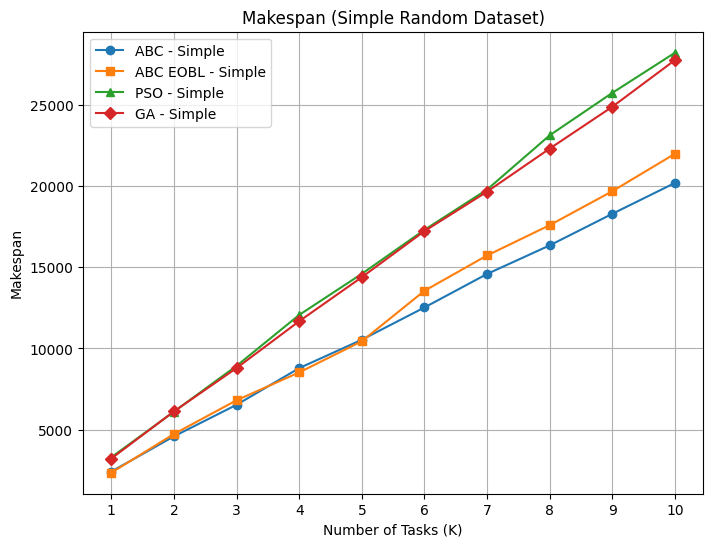
\includegraphics[width=0.75\linewidth]{gambar/Grafik Makespan Simple Random.png}
    \caption{Grafik \textit{makespan simple random}}
\end{figure}

\newpage

\begin{figure} [H]
    \centering
    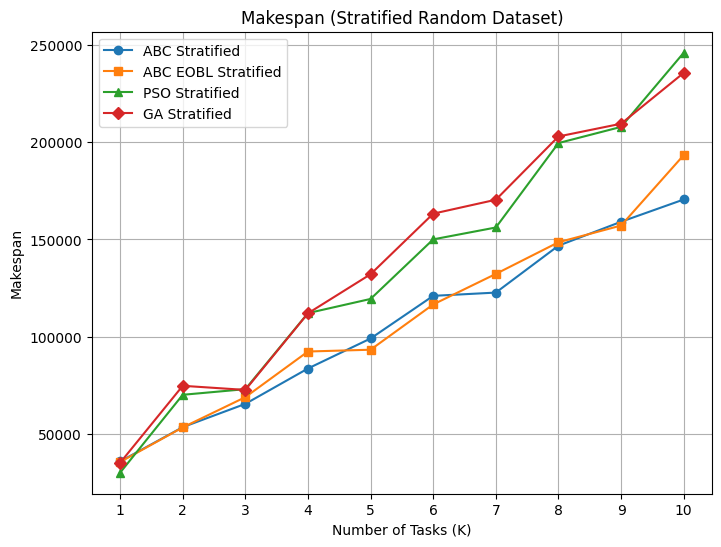
\includegraphics[width=0.75\linewidth]{gambar/Grafik Makespan Stratified Random.png}
    \caption{Grafik \textit{makespan stratified random}}
\end{figure}

\begin{figure} [H]
    \centering
    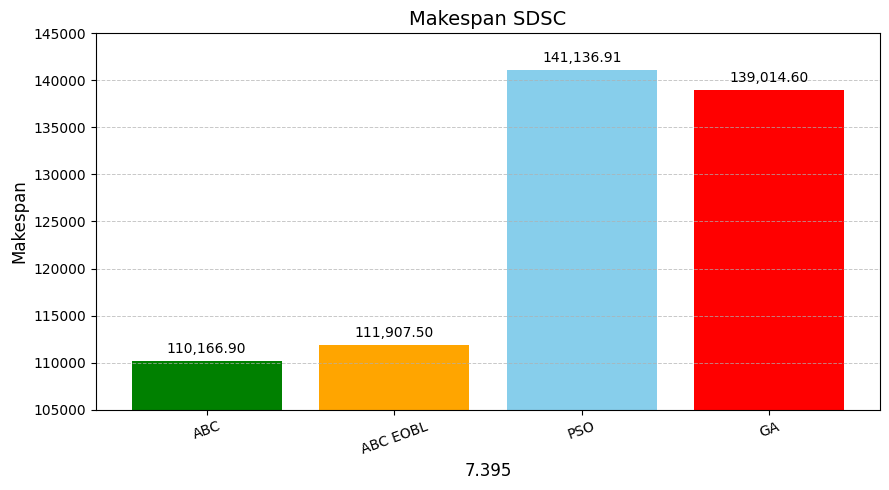
\includegraphics[width=0.75\linewidth]{gambar/Grafik Makespan SDSC.png}
    \caption{Grafik \textit{makespan} SDSC}
\end{figure}

\newpage

\begin{figure} [H]
    \centering
    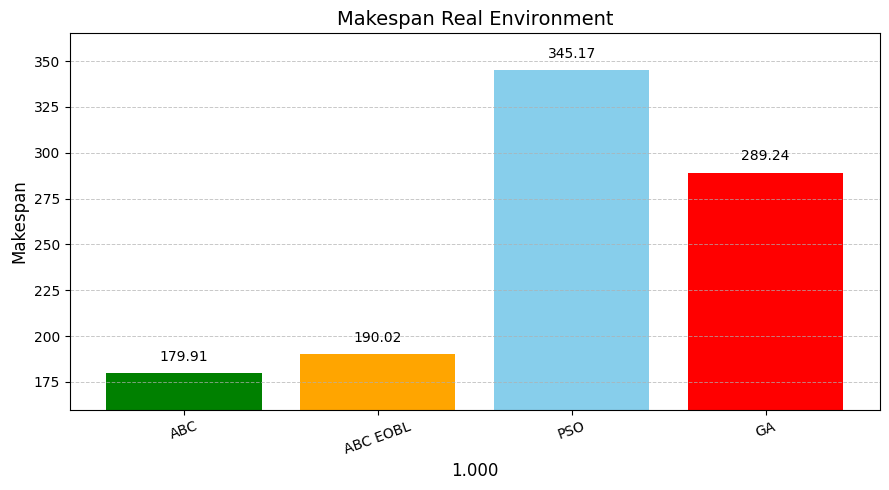
\includegraphics[width=0.75\linewidth]{gambar/Grafik Makespan Real Environment.png}
    \caption{Grafik \textit{makespan real environment}}
\end{figure}

\subsection{\textit{Average Start Time} (\textit{Lower Better})}
\textit{Average start time} mengacu pada waktu rata-rata yang diperlukan oleh algoritma untuk memulai eksekusi sebuah tugas pada lingkungan \textit{cloud}. Semakin rendah nilai \textit{average start time}, maka semakin baik kinerja algoritma tersebut dalam hal efisiensi waktu inisiasi tugas.

\begin{table} [H]
\centering
\caption{\textit{Average start time simple random}}
\begin{tabular}{|>{\raggedleft\arraybackslash}m{0.12\linewidth}|
                >{\raggedleft\arraybackslash}m{0.17\linewidth}|
                >{\raggedleft\arraybackslash}m{0.17\linewidth}|
                >{\raggedleft\arraybackslash}m{0.17\linewidth}|
                >{\raggedleft\arraybackslash}m{0.17\linewidth}|}
\rowcolor{blue!30}
\hline
\multicolumn{1}{|>{\centering\arraybackslash}m{0.12\linewidth}|}{\textbf{\textit{Cloudlets}}} & 
\multicolumn{1}{>{\centering\arraybackslash}m{0.17\linewidth}|}{\textbf{ABC \textit{Simple}}} & 
\multicolumn{1}{>{\centering\arraybackslash}m{0.17\linewidth}|}{\textbf{ABC EOBL \textit{Simple}}} & 
\multicolumn{1}{>{\centering\arraybackslash}m{0.17\linewidth}|}{\textbf{PSO \textit{Simple}}} & 
\multicolumn{1}{>{\centering\arraybackslash}m{0.17\linewidth}|}{\textbf{GA \textit{Simple}}} \\
\hline
1.000 & 738,30 & 732,27 & 1.008,53 & 1.097,42 \\
\hline
2.000 & 1.074,04 & 1.500,95 & 2.064,80 & 2.277,04 \\
\hline
3.000 & 2.246,88 & 2.245,16 & 3.056,15 & 3.380,23 \\
\hline
4.000 & 2.981,69 & 2.967,65 & 4.137,20 & 4.537,59 \\
\hline
5.000 & 3.700,48 & 3.676,07 & 5.142,45 & 5.597,77 \\
\hline
6.000 & 4.454,43 & 4.600,88 & 6.199,46 & 6.786,18 \\
\hline
7.000 & 5.200,75 & 5.380,87 & 7.153,93 & 7.863,54 \\
\hline
8.000 & 5.978,64 & 6.155,85 & 8.291,67 & 9.049,82 \\
\hline
9.000 & 6.714,10 & 6.910,13 & 9.288,67 & 10.157,47 \\
\hline
10.000 & 7.425,45 & 7.672,21 & 10.333,42 & 11.318,84 \\
\hline
\textbf{AVG} & \textcolor{green}{4.051,48} & 4.184,20 & 5.667,63 & 6.206,59 \\
\hline
\end{tabular}
\end{table}

\newpage

\begin{table} [H]
\centering
\caption{\textit{Average start time stratified random}}
\begin{tabular}{|>{\raggedleft\arraybackslash}m{0.12\linewidth}|
                >{\raggedleft\arraybackslash}m{0.17\linewidth}|
                >{\raggedleft\arraybackslash}m{0.17\linewidth}|
                >{\raggedleft\arraybackslash}m{0.17\linewidth}|
                >{\raggedleft\arraybackslash}m{0.17\linewidth}|}
\rowcolor{blue!30}
\hline
\multicolumn{1}{|>{\centering\arraybackslash}m{0.12\linewidth}|}{\textbf{\textit{Cloudlets}}} & 
\multicolumn{1}{>{\centering\arraybackslash}m{0.17\linewidth}|}{\textbf{ABC \textit{Stratified}}} & 
\multicolumn{1}{>{\centering\arraybackslash}m{0.17\linewidth}|}{\textbf{ABC EOBL \textit{Stratified}}} & 
\multicolumn{1}{>{\centering\arraybackslash}m{0.17\linewidth}|}{\textbf{PSO \textit{Stratified}}} & 
\multicolumn{1}{>{\centering\arraybackslash}m{0.17\linewidth}|}{\textbf{GA \textit{Stratified}}} \\
\hline
1.000 & 4.640,92 & 4.792,01 & 5.503,25 & 5.739,04 \\
\hline
2.000 & 10.177,47 & 10.785,78 & 14.849,58 & 16.087,73 \\
\hline
3.000 & 14.791,98 & 14.845,95 & 19.424,48 & 20.590,21 \\
\hline
4.000 & 20.742,34 & 21.314,79 & 28.380,60 & 32.214,32 \\
\hline
5.000 & 25.006,78 & 26.142,43 & 33.360,28 & 37.442,09 \\
\hline
6.000 & 31.639,72 & 31.604,86 & 43.449,62 & 48.034,96 \\
\hline
7.000 & 35.668,25 & 36.673,71 & 46.601,23 & 51.228,05 \\
\hline
8.000 & 41.471,38 & 43.314,06 & 58.719,59 & 63.714,31 \\
\hline
9.000 & 46.771,80 & 46.972,56 & 62.034,10 & 68.314,65 \\
\hline
10.000 & 51.402,64 & 54.759,20 & 72.289,93 & 79.753,82 \\
\hline
\textbf{AVG} & \textcolor{green}{28.231,33} & 29.120,54 & 38.461,27 & 42.311,92 \\
\hline
\end{tabular}
\end{table}

\begin{table} [H]
\centering
\caption{\textit{Average start time} SDSC}
\begin{tabular}{|>{\raggedleft\arraybackslash}m{0.12\linewidth}|
                >{\raggedleft\arraybackslash}m{0.15\linewidth}|
                >{\raggedleft\arraybackslash}m{0.25\linewidth}|
                >{\raggedleft\arraybackslash}m{0.15\linewidth}|
                >{\raggedleft\arraybackslash}m{0.15\linewidth}|}
\rowcolor{blue!30}
\hline
\multicolumn{1}{|>{\centering\arraybackslash}m{0.12\linewidth}|}{\textbf{\textit{Cloudlets}}} & 
\multicolumn{1}{>{\centering\arraybackslash}m{0.15\linewidth}|}{\textbf{ABC SDSC}} & 
\multicolumn{1}{>{\centering\arraybackslash}m{0.25\linewidth}|}{\textbf{ABC EOBL SDSC}} & 
\multicolumn{1}{>{\centering\arraybackslash}m{0.15\linewidth}|}{\textbf{PSO SDSC}} & 
\multicolumn{1}{>{\centering\arraybackslash}m{0.15\linewidth}|}{\textbf{GA SDSC}} \\
\hline
7.395 & \textcolor{green}{27.926,11} & 28.538,28 & 37.766,73 & 41.644,38\\
\hline
\end{tabular}
\end{table}

\begin{table} [H]
\centering
\caption{\textit{Average start time real environment}}
\begin{tabular}{|>{\raggedleft\arraybackslash}m{0.1\linewidth}|
                >{\raggedleft\arraybackslash}m{0.17\linewidth}|
                >{\raggedleft\arraybackslash}m{0.17\linewidth}|
                >{\raggedleft\arraybackslash}m{0.17\linewidth}|
                >{\raggedleft\arraybackslash}m{0.17\linewidth}|}
\rowcolor{blue!30}
\hline
\multicolumn{1}{|>{\centering\arraybackslash}m{0.1\linewidth}|}{\textbf{\textit{Task}}} & 
\multicolumn{1}{>{\centering\arraybackslash}m{0.17\linewidth}|}{\textbf{ABC RE}} & 
\multicolumn{1}{>{\centering\arraybackslash}m{0.17\linewidth}|}{\textbf{ABC EOBL RE}} & 
\multicolumn{1}{>{\centering\arraybackslash}m{0.17\linewidth}|}{\textbf{PSO RE}} & 
\multicolumn{1}{>{\centering\arraybackslash}m{0.17\linewidth}|}{\textbf{GA RE}} \\
\hline
1.000 & \textcolor{green}{89.620,01} & 92.554,11 & 196.952,51 & 144.562,97 \\
\hline
\end{tabular}
\end{table}

Berdasarkan hasil pengujian yang ditampilkan pada tabel dan grafik eksperimen, algoritma \textit{Artificial Bee Colony} (ABC) menunjukkan performa yang lebih baik dengan menghasilkan nilai \textit{average start time} paling rendah dibandingkan dengan algoritma ABC yang dikombinasikan dengan \textit{Elite Opposition-Based Learning} (ABC-EOBL). Hal ini konsisten terlihat pada \textit{dataset simple random}, \textit{stratified random}, maupun SDSC.

Penyebab utama meningkatnya nilai \textit{average start time} pada algoritma ABC-EOBL adalah kompleksitas tambahan yang dimiliki oleh pendekatan EOBL, terutama proses evaluasi solusi lawan yang secara signifikan menambah waktu komputasi. Kondisi ini menyebabkan waktu inisiasi eksekusi tugas menjadi lebih lama dibandingkan dengan algoritma ABC yang lebih sederhana, sehingga meningkatkan nilai \textit{average start time} pada ABC-EOBL.

\newpage

\begin{figure} [H]
    \centering
    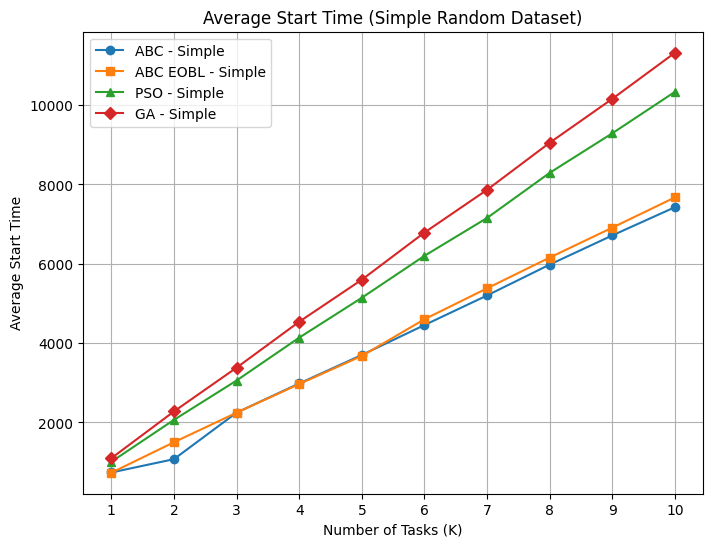
\includegraphics[width=0.75\linewidth]{gambar/Grafik Average Start Time Simple Random.png}
    \caption{Grafik \textit{average start time simple random}}
\end{figure}

\begin{figure} [H]
    \centering
    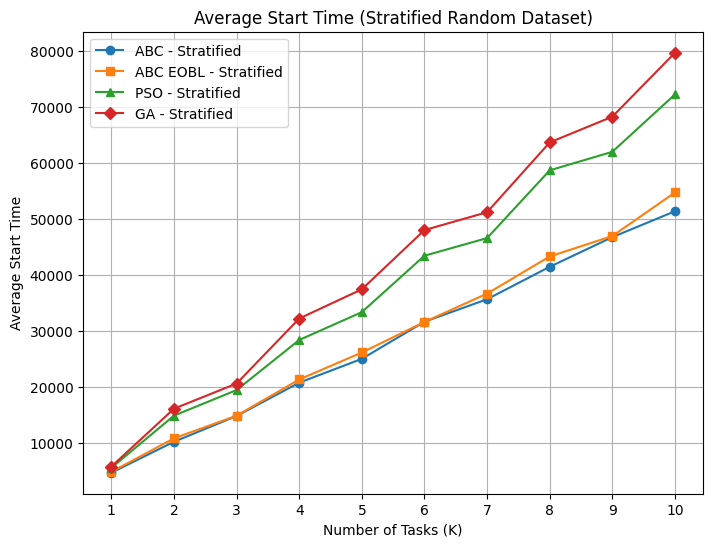
\includegraphics[width=0.75\linewidth]{gambar/Grafik Average Start Time Stratified Random.png}
    \caption{Grafik \textit{average start time stratified random}}
\end{figure}

\newpage

\begin{figure} [H]
    \centering
    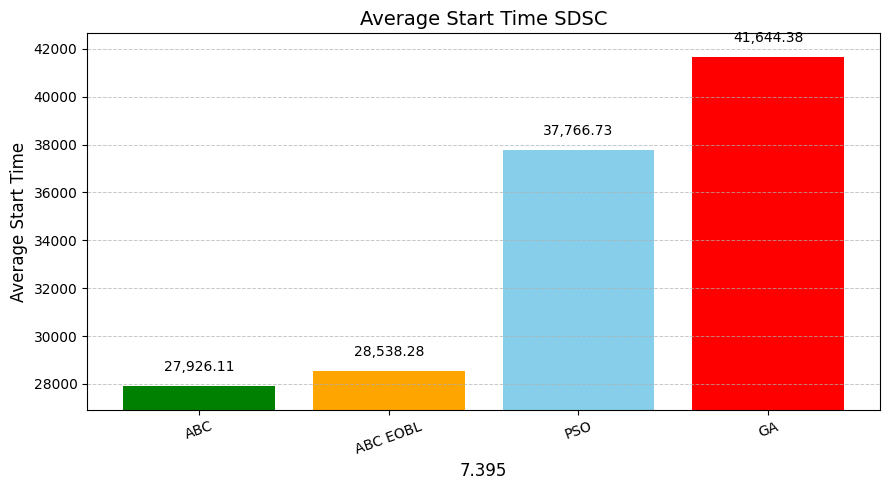
\includegraphics[width=0.75\linewidth]{gambar/Grafik Average Start Time SDSC.png}
    \caption{Grafik \textit{average start time} SDSC}
\end{figure}

\begin{figure} [H]
    \centering
    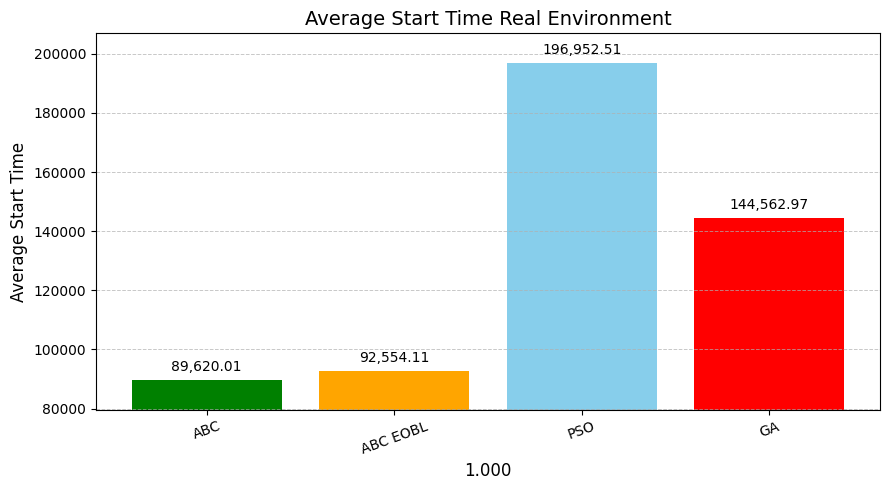
\includegraphics[width=0.75\linewidth]{gambar/Grafik Average Start Time Real Environment.png}
    \caption{Grafik \textit{average start time real environment}}
\end{figure}

\subsection{\textit{Average Finish Time} (\textit{Lower Better})}
\textit{Average finish time} adalah rata-rata waktu yang diperlukan oleh algoritma untuk menyelesaikan eksekusi suatu tugas pada lingkungan \textit{cloud}. Semakin rendah nilai \textit{average finish time}, semakin baik performa algoritma dalam hal efisiensi penyelesaian tugas.

\newpage

\begin{table} [H]
\centering
\caption{\textit{Average finish time simple random}}
\begin{tabular}{|>{\raggedleft\arraybackslash}m{0.12\linewidth}|
                >{\raggedleft\arraybackslash}m{0.17\linewidth}|
                >{\raggedleft\arraybackslash}m{0.17\linewidth}|
                >{\raggedleft\arraybackslash}m{0.17\linewidth}|
                >{\raggedleft\arraybackslash}m{0.17\linewidth}|}
\rowcolor{blue!30}
\hline
\multicolumn{1}{|>{\centering\arraybackslash}m{0.12\linewidth}|}{\textbf{\textit{Cloudlets}}} & 
\multicolumn{1}{>{\centering\arraybackslash}m{0.17\linewidth}|}{\textbf{ABC \textit{Simple}}} & 
\multicolumn{1}{>{\centering\arraybackslash}m{0.17\linewidth}|}{\textbf{ABC EOBL \textit{Simple}}} & 
\multicolumn{1}{>{\centering\arraybackslash}m{0.17\linewidth}|}{\textbf{PSO \textit{Simple}}} & 
\multicolumn{1}{>{\centering\arraybackslash}m{0.17\linewidth}|}{\textbf{GA \textit{Simple}}} \\
\hline
1.000 & 744,15 & 792,42 & 1.066,07 & 1.154,04 \\
\hline
2.000 & 1.155,26 & 1.560,74 & 2.121,92 & 2.333,22 \\
\hline
3.000 & 2.306,88 & 2.305,15 & 3.113,53 & 3.436,73 \\
\hline
4.000 & 3.041,32 & 3.027,39 & 4.194,14 & 4.593,67 \\
\hline
5.000 & 3.760,12 & 3.735,78 & 5.199,39 & 5.653,89 \\
\hline
6.000 & 4.514,15 & 4.660,33 & 6.256,46 & 6.842,31 \\
\hline
7.000 & 5.260,52 & 5.440,37 & 7.211,08 & 7.919,79 \\
\hline
8.000 & 6.038,45 & 6.215,45 & 8.348,82 & 9.106,11 \\
\hline
9.000 & 6.773,92 & 6.969,75 & 9.345,81 & 10.213,75 \\
\hline
10.000 & 7.485,23 & 7.731,69 & 10.390,46 & 11.375,02 \\
\hline
\textbf{AVG} & \textcolor{green}{4.108,00} & 4.243,91 & 5.724,77 & 6.262,85 \\
\hline
\end{tabular}
\end{table}

\begin{table} [H]
\centering
\caption{\textit{Average finish time stratified random}}
\begin{tabular}{|>{\raggedleft\arraybackslash}m{0.12\linewidth}|
                >{\raggedleft\arraybackslash}m{0.17\linewidth}|
                >{\raggedleft\arraybackslash}m{0.17\linewidth}|
                >{\raggedleft\arraybackslash}m{0.17\linewidth}|
                >{\raggedleft\arraybackslash}m{0.17\linewidth}|}
\rowcolor{blue!30}
\hline
\multicolumn{1}{|>{\centering\arraybackslash}m{0.12\linewidth}|}{\textbf{\textit{Cloudlets}}} & 
\multicolumn{1}{>{\centering\arraybackslash}m{0.17\linewidth}|}{\textbf{ABC \textit{Stratified}}} & 
\multicolumn{1}{>{\centering\arraybackslash}m{0.17\linewidth}|}{\textbf{ABC EOBL \textit{Stratified}}} & 
\multicolumn{1}{>{\centering\arraybackslash}m{0.17\linewidth}|}{\textbf{PSO \textit{Stratified}}} & 
\multicolumn{1}{>{\centering\arraybackslash}m{0.17\linewidth}|}{\textbf{GA \textit{Stratified}}} \\
\hline
1.000 & 5.129,75 & 5.269,51 & 5.973,21 & 6.209,89 \\
\hline
2.000 & 10.641,35 & 11.243,58 & 15.286,22 & 16.517,60 \\
\hline
3.000 & 15.266,41 & 15.322,64 & 19.881,74 & 21.040,78 \\
\hline
4.000 & 21.205,64 & 21.776,03 & 28.819,61 & 32.645,10 \\
\hline
5.000 & 25.477,13 & 26.611,62 & 33.812,72 & 37.883,78 \\
\hline
6.000 & 32.102,34 & 32.066,59 & 43.887,95 & 48.464,10 \\
\hline
7.000 & 36.135,94 & 37.140,14 & 47.049,03 & 51.667,85 \\
\hline
8.000 & 41.935,48 & 43.776,96 & 59.159,66 & 64.145,57 \\
\hline
9.000 & 47.237,64 & 47.440,02 & 62.480,53 & 68.752,49 \\
\hline
10.000 & 51.865,55 & 55.217,92 & 72.728,10 & 80.183,74 \\
\hline
\textbf{AVG} & \textcolor{green}{28.699,72} & 29.586,50 & 38.907,88 & 42.751,09 \\
\hline
\end{tabular}
\end{table}

\begin{table} [H]
\centering
\caption{\textit{Average finish time} SDSC}
\begin{tabular}{|>{\raggedleft\arraybackslash}m{0.12\linewidth}|
                >{\raggedleft\arraybackslash}m{0.15\linewidth}|
                >{\raggedleft\arraybackslash}m{0.25\linewidth}|
                >{\raggedleft\arraybackslash}m{0.15\linewidth}|
                >{\raggedleft\arraybackslash}m{0.15\linewidth}|}
\rowcolor{blue!30}
\hline
\multicolumn{1}{|>{\centering\arraybackslash}m{0.12\linewidth}|}{\textbf{\textit{Cloudlets}}} & 
\multicolumn{1}{>{\centering\arraybackslash}m{0.15\linewidth}|}{\textbf{ABC SDSC}} & 
\multicolumn{1}{>{\centering\arraybackslash}m{0.25\linewidth}|}{\textbf{ABC EOBL SDSC}} & 
\multicolumn{1}{>{\centering\arraybackslash}m{0.15\linewidth}|}{\textbf{PSO SDSC}} & 
\multicolumn{1}{>{\centering\arraybackslash}m{0.15\linewidth}|}{\textbf{GA SDSC}} \\
\hline
7.395 & \textcolor{green}{28.277,85} & 28.888,60 & 38.102,26 & 41.970,13 \\
\hline
\end{tabular}
\end{table}

\begin{table} [H]
\centering
\caption{\textit{Average finish time real environment}}
\begin{tabular}{|>{\raggedleft\arraybackslash}m{0.1\linewidth}|
                >{\raggedleft\arraybackslash}m{0.17\linewidth}|
                >{\raggedleft\arraybackslash}m{0.17\linewidth}|
                >{\raggedleft\arraybackslash}m{0.17\linewidth}|
                >{\raggedleft\arraybackslash}m{0.17\linewidth}|}
\rowcolor{blue!30}
\hline
\multicolumn{1}{|>{\centering\arraybackslash}m{0.1\linewidth}|}{\textbf{\textit{Task}}} & 
\multicolumn{1}{>{\centering\arraybackslash}m{0.17\linewidth}|}{\textbf{ABC RE}} & 
\multicolumn{1}{>{\centering\arraybackslash}m{0.17\linewidth}|}{\textbf{ABC EOBL RE}} & 
\multicolumn{1}{>{\centering\arraybackslash}m{0.17\linewidth}|}{\textbf{PSO RE}} & 
\multicolumn{1}{>{\centering\arraybackslash}m{0.17\linewidth}|}{\textbf{GA RE}} \\
\hline
1.000 & \textcolor{green}{89.783,92} & 92.722,07 & 197.276,29 & 144.789,12 \\
\hline
\end{tabular}
\end{table}

Berdasarkan hasil pengujian pada tabel dan grafik eksperimen, algoritma \textit{Artificial Bee Colony} (ABC) menunjukkan nilai \textit{average finish time} paling rendah secara konsisten dibandingkan dengan algoritma ABC yang dikombinasikan dengan \textit{Elite Opposition-Based Learning} (EOBL). Pada \textit{dataset simple random}, ABC secara jelas menunjukkan performa terbaik dengan waktu penyelesaian rata-rata yang lebih cepat dibandingkan ABC-EOBL. Kondisi serupa juga terlihat pada \textit{dataset stratified random}, di mana ABC tanpa modifikasi mampu menyelesaikan tugas lebih efisien dibandingkan dengan algoritma ABC-EOBL.

Penyebab utama nilai \textit{average finish time} yang lebih tinggi pada algoritma ABC-EOBL adalah kompleksitas tambahan dari metode \textit{Elite Opposition-Based Learning}. Metode ini memerlukan evaluasi tambahan terhadap solusi lawan, yang menyebabkan waktu komputasi lebih lama dan memperlambat konvergensi menuju solusi optimal. Akibatnya, algoritma membutuhkan waktu lebih lama untuk menyelesaikan eksekusi tugas.

\begin{figure} [H]
    \centering
    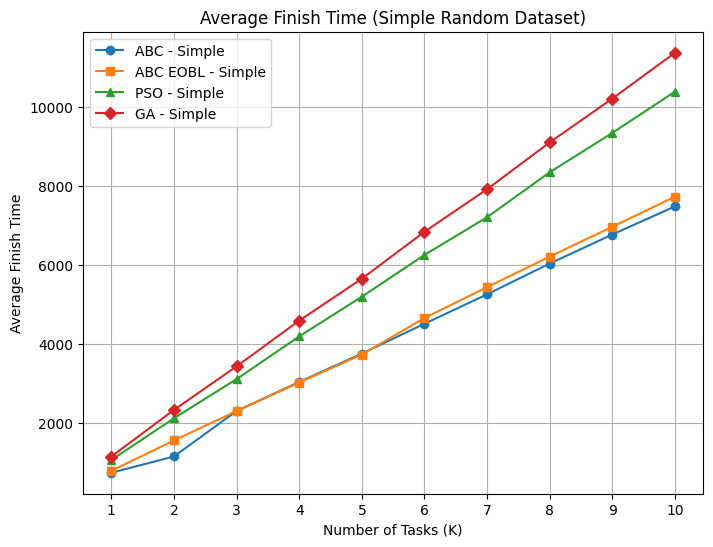
\includegraphics[width=0.75\linewidth]{gambar/Grafik Average Finish Time Simple Random.png}
    \caption{Grafik \textit{average finish time simple random}}
\end{figure}

\newpage

\begin{figure} [H]
    \centering
    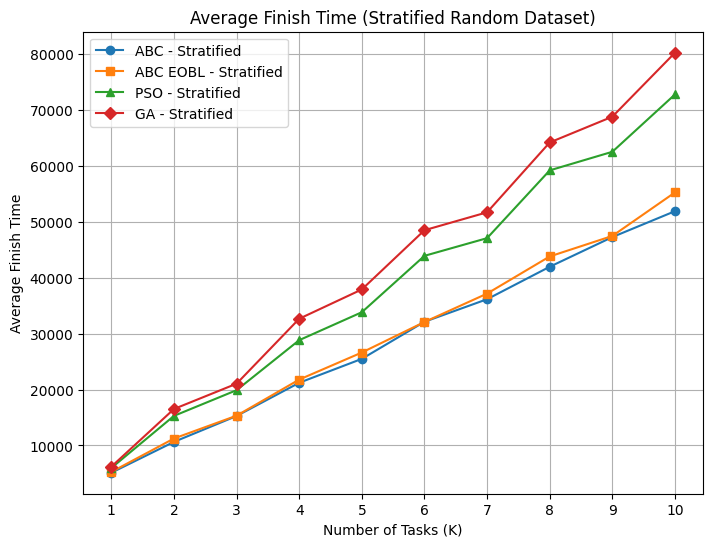
\includegraphics[width=0.75\linewidth]{gambar/Grafik Average Finish Time Stratified Random.png}
    \caption{Grafik \textit{average finish time stratified random}}
\end{figure}

\begin{figure} [H]
    \centering
    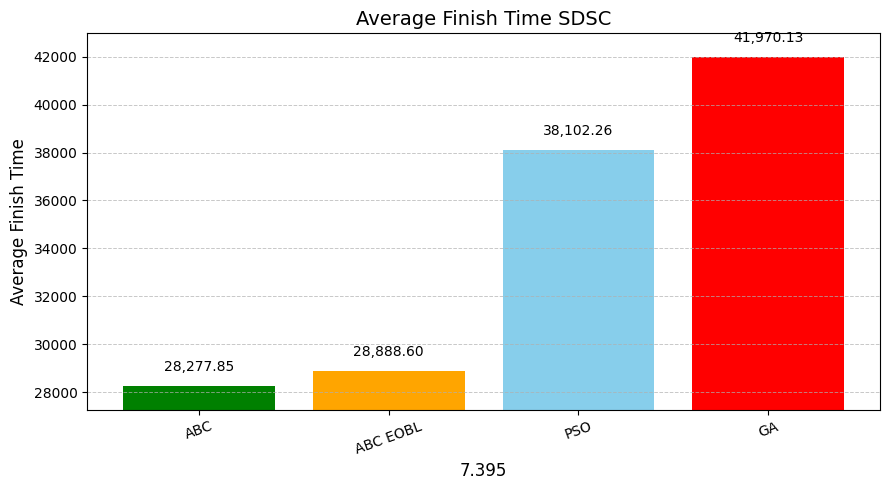
\includegraphics[width=0.75\linewidth]{gambar/Grafik Average Finish Time SDSC.png}
    \caption{Grafik \textit{average finish time} SDSC}
\end{figure}

\newpage

\begin{figure} [H]
    \centering
    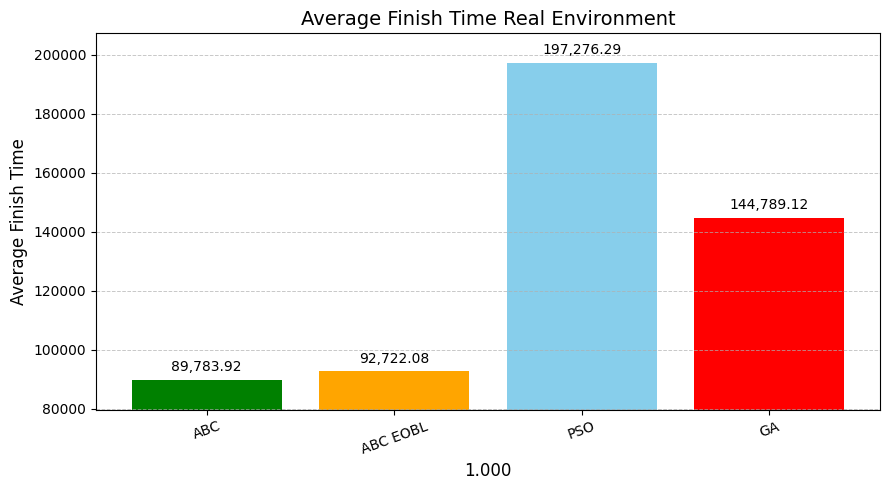
\includegraphics[width=0.75\linewidth]{gambar/Grafik Average Finish Time Real Environment.png}
    \caption{Grafik \textit{average finish time real environment}}
\end{figure}

\subsection{\textit{Average Execution Time} (\textit{Lower Better})}
\textit{Average execution time} merujuk pada waktu rata-rata yang dibutuhkan algoritma untuk menyelesaikan proses eksekusi sebuah tugas pada lingkungan \textit{cloud}. Semakin rendah nilai \textit{average execution time}, semakin baik efisiensi algoritma dalam menjalankan tugas-tugas tersebut.

\begin{table} [H]
\centering
\caption{\textit{Average execution time simple random}}
\begin{tabular}{|>{\raggedleft\arraybackslash}m{0.12\linewidth}|
                >{\raggedleft\arraybackslash}m{0.17\linewidth}|
                >{\raggedleft\arraybackslash}m{0.17\linewidth}|
                >{\raggedleft\arraybackslash}m{0.17\linewidth}|
                >{\raggedleft\arraybackslash}m{0.17\linewidth}|}
\rowcolor{blue!30}
\hline
\multicolumn{1}{|>{\centering\arraybackslash}m{0.12\linewidth}|}{\textbf{\textit{Cloudlets}}} & 
\multicolumn{1}{>{\centering\arraybackslash}m{0.17\linewidth}|}{\textbf{ABC \textit{Simple}}} & 
\multicolumn{1}{>{\centering\arraybackslash}m{0.17\linewidth}|}{\textbf{ABC EOBL \textit{Simple}}} & 
\multicolumn{1}{>{\centering\arraybackslash}m{0.17\linewidth}|}{\textbf{PSO \textit{Simple}}} & 
\multicolumn{1}{>{\centering\arraybackslash}m{0.17\linewidth}|}{\textbf{GA \textit{Simple}}} \\
\hline
1.000 & 59,90 & 60,15 & 57,54 & 56,62 \\
\hline
2.000 & 59,70 & 59,79 & 57,12 & 56,19 \\
\hline
3.000 & 60,00 & 59,99 & 57,38 & 56,49 \\
\hline
4.000 & 59,62 & 59,74 & 56,94 & 56,08 \\
\hline
5.000 & 59,64 & 59,71 & 56,94 & 56,12 \\
\hline
6.000 & 59,71 & 59,45 & 57,00 & 56,13 \\
\hline
7.000 & 59,78 & 59,50 & 57,15 & 56,25 \\
\hline
8.000 & 59,81 & 59,59 & 57,16 & 56,29 \\
\hline
9.000 & 59,82 & 59,61 & 57,15 & 56,28 \\
\hline
10.000 & 59,78 & 59,48 & 57,04 & 56,17 \\
\hline
\textbf{AVG} & 59,78 & 59,70 & 57,14 & \textcolor{green}{56,26} \\
\hline
\end{tabular}
\end{table}

\newpage

\begin{table} [H]
\centering
\caption{\textit{Average execution time stratified random}}
\begin{tabular}{|>{\raggedleft\arraybackslash}m{0.12\linewidth}|
                >{\raggedleft\arraybackslash}m{0.17\linewidth}|
                >{\raggedleft\arraybackslash}m{0.17\linewidth}|
                >{\raggedleft\arraybackslash}m{0.17\linewidth}|
                >{\raggedleft\arraybackslash}m{0.17\linewidth}|}
\rowcolor{blue!30}
\hline
\multicolumn{1}{|>{\centering\arraybackslash}m{0.12\linewidth}|}{\textbf{\textit{Cloudlets}}} & 
\multicolumn{1}{>{\centering\arraybackslash}m{0.17\linewidth}|}{\textbf{ABC \textit{Stratified}}} & 
\multicolumn{1}{>{\centering\arraybackslash}m{0.17\linewidth}|}{\textbf{ABC EOBL \textit{Stratified}}} & 
\multicolumn{1}{>{\centering\arraybackslash}m{0.17\linewidth}|}{\textbf{PSO \textit{Stratified}}} & 
\multicolumn{1}{>{\centering\arraybackslash}m{0.17\linewidth}|}{\textbf{GA \textit{Stratified}}} \\
\hline
1.000 & 488,83 & 477,50 & 469,97 & 470,85 \\
\hline
2.000 & 463,88 & 457,80 & 436,64 & 429,87 \\
\hline
3.000 & 474,44 & 476,69 & 457,27 & 450,56 \\
\hline
4.000 & 463,30 & 461,25 & 439,00 & 430,78 \\
\hline
5.000 & 470,35 & 469,19 & 452,44 & 441,69 \\
\hline
6.000 & 462,62 & 461,73 & 438,33 & 429,15 \\
\hline
7.000 & 467,69 & 466,43 & 447,79 & 439,80 \\
\hline
8.000 & 464,10 & 462,90 & 440,07 & 431,27 \\
\hline
9.000 & 465,85 & 467,46 & 446,43 & 437,84 \\
\hline
10.000 & 462,91 & 458,73 & 438,17 & 429,92 \\
\hline
\textbf{AVG} & 468,40 & 465,97 & 446,61 & \textcolor{green}{439,17} \\
\hline
\end{tabular}
\end{table}

\begin{table} [H]
\centering
\caption{\textit{Average execution time} SDSC}
\begin{tabular}{|>{\raggedleft\arraybackslash}m{0.12\linewidth}|
                >{\raggedleft\arraybackslash}m{0.15\linewidth}|
                >{\raggedleft\arraybackslash}m{0.25\linewidth}|
                >{\raggedleft\arraybackslash}m{0.15\linewidth}|
                >{\raggedleft\arraybackslash}m{0.15\linewidth}|}
\rowcolor{blue!30}
\hline
\multicolumn{1}{|>{\centering\arraybackslash}m{0.12\linewidth}|}{\textbf{Cloudlets}} & 
\multicolumn{1}{>{\centering\arraybackslash}m{0.15\linewidth}|}{\textbf{ABC SDSC}} & 
\multicolumn{1}{>{\centering\arraybackslash}m{0.25\linewidth}|}{\textbf{ABC EOBL SDSC}} & 
\multicolumn{1}{>{\centering\arraybackslash}m{0.15\linewidth}|}{\textbf{PSO SDSC}} & 
\multicolumn{1}{>{\centering\arraybackslash}m{0.15\linewidth}|}{\textbf{GA SDSC}} \\
\hline
7.395 & 351,73 & 350,31 & 335,53 & \textcolor{green}{325,75} \\
\hline
\end{tabular}
\end{table}

\begin{table} [H]
\centering
\caption{\textit{Average execution time real environment}}
\begin{tabular}{|>{\raggedleft\arraybackslash}m{0.1\linewidth}|
                >{\raggedleft\arraybackslash}m{0.17\linewidth}|
                >{\raggedleft\arraybackslash}m{0.17\linewidth}|
                >{\raggedleft\arraybackslash}m{0.17\linewidth}|
                >{\raggedleft\arraybackslash}m{0.17\linewidth}|}
\rowcolor{blue!30}
\hline
\multicolumn{1}{|>{\centering\arraybackslash}m{0.1\linewidth}|}{\textbf{\textit{Task}}} & 
\multicolumn{1}{>{\centering\arraybackslash}m{0.17\linewidth}|}{\textbf{ABC RE}} & 
\multicolumn{1}{>{\centering\arraybackslash}m{0.17\linewidth}|}{\textbf{ABC EOBL RE}} & 
\multicolumn{1}{>{\centering\arraybackslash}m{0.17\linewidth}|}{\textbf{PSO RE}} & 
\multicolumn{1}{>{\centering\arraybackslash}m{0.17\linewidth}|}{\textbf{GA RE}} \\
\hline
1.000 & \textcolor{green}{163,91} & 167,966 & 323,78 & 226.15 \\
\hline
\end{tabular}
\end{table}

Berdasarkan hasil eksperimen yang disajikan dalam tabel dan grafik, terlihat bahwa Genetic Algorithm (GA) secara konsisten menunjukkan nilai Average Execution Time terendah pada seluruh dataset yang diuji, mengindikasikan efisiensi eksekusi tugas yang paling tinggi dibandingkan algoritma lainnya. Kemudian, algoritma Artificial Bee Colony dengan Elite Opposition-Based Learning (ABC-EOBL) menempati posisi ketiga setelah Particle Swarm Optimization (PSO), dengan waktu eksekusi rata-rata yang sedikit lebih tinggi dibandingkan PSO namun lebih rendah daripada algoritma ABC.

Algoritma ABC memiliki nilai Average Execution Time tertinggi, menunjukkan bahwa algoritma ini membutuhkan waktu paling lama dalam menyelesaikan eksekusi tugas. Penyebab utama dari perbedaan ini adalah algoritma ABC yang tidak memiliki mekanisme pencarian adaptif seefisien GA dan PSO ataupun mekanisme diversifikasi solusi yang dimiliki ABC-EOBL, sehingga proses pencarian solusi optimal menjadi lebih lama.

\newpage

\begin{figure} [H]
    \centering
    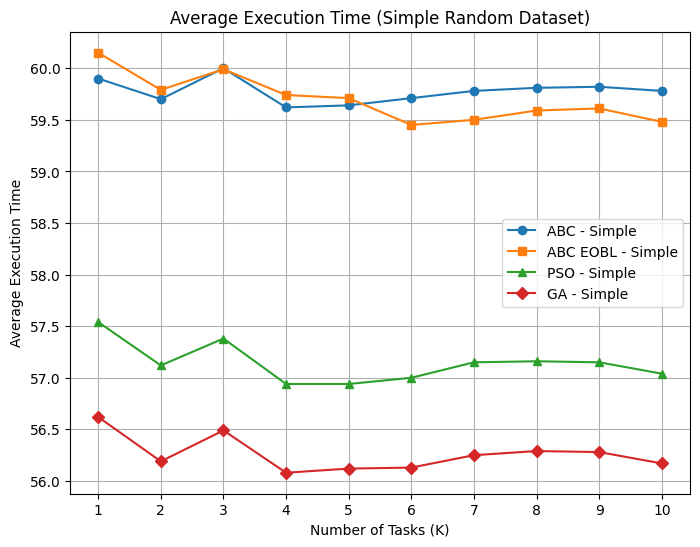
\includegraphics[width=0.75\linewidth]{gambar/Grafik Average Execution Time Simple Random.png}
    \caption{Grafik \textit{average execution time simple random}}
\end{figure}

\begin{figure} [H]
    \centering
    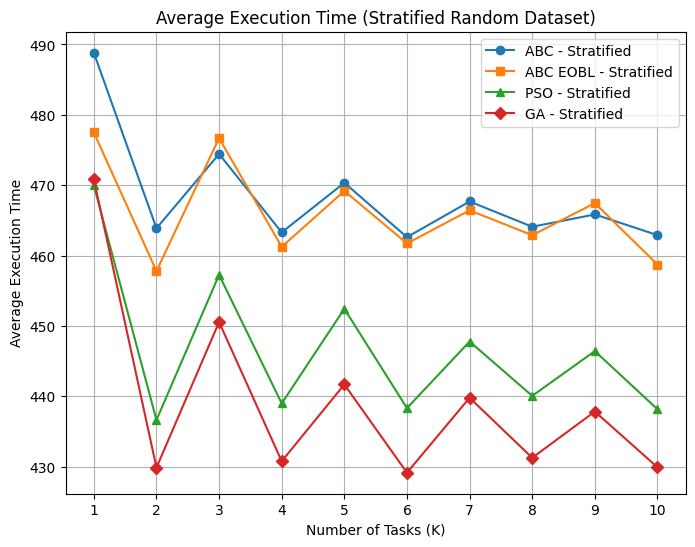
\includegraphics[width=0.75\linewidth]{gambar/Grafik Average Execution Time Stratified Random.png}
    \caption{Grafik \textit{average execution time stratified random}}
\end{figure}

\newpage

\begin{figure} [H]
    \centering
    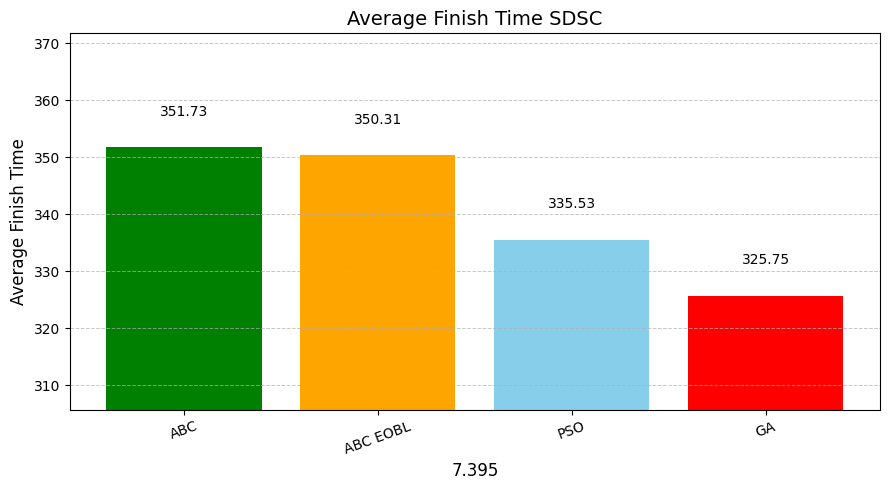
\includegraphics[width=0.75\linewidth]{gambar/Grafik Average Execution Time SDSC.png}
    \caption{Grafik \textit{average execution time} SDSC}
\end{figure}

\begin{figure} [H]
    \centering
    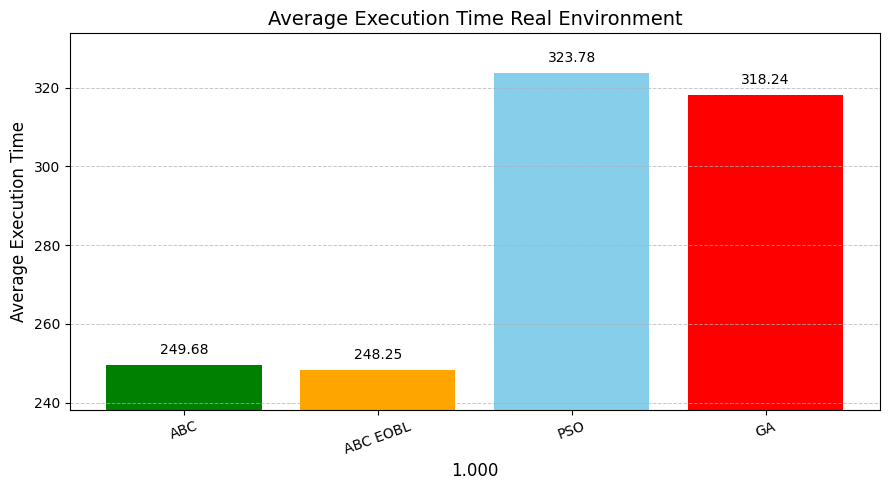
\includegraphics[width=0.75\linewidth]{gambar/Grafik Average Execution Time Real Environment.png}
    \caption{Grafik \textit{average execution time real environment}}
\end{figure}

\subsection{\textit{Average Waiting Time} (\textit{Lower Better})}
\textit{Average waiting time} mengacu pada waktu rata-rata yang dihabiskan oleh setiap tugas dalam antrian sebelum diproses oleh \textit{virtual machine}. Semakin rendah nilai \textit{average waiting time}, maka semakin efisien algoritma dalam mengatur dan mendistribusikan penjadwalan tugas.

\newpage

\begin{table} [H]
\centering
\caption{Average waiting time simple random}
\begin{tabular}{|>{\raggedleft\arraybackslash}m{0.12\linewidth}|
                >{\raggedleft\arraybackslash}m{0.17\linewidth}|
                >{\raggedleft\arraybackslash}m{0.17\linewidth}|
                >{\raggedleft\arraybackslash}m{0.17\linewidth}|
                >{\raggedleft\arraybackslash}m{0.17\linewidth}|}
\rowcolor{blue!30}
\hline
\multicolumn{1}{|>{\centering\arraybackslash}m{0.12\linewidth}|}{\textbf{\textit{Cloudlets}}} & 
\multicolumn{1}{>{\centering\arraybackslash}m{0.17\linewidth}|}{\textbf{ABC \textit{Simple}}} & 
\multicolumn{1}{>{\centering\arraybackslash}m{0.17\linewidth}|}{\textbf{ABC EOBL \textit{Simple}}} & 
\multicolumn{1}{>{\centering\arraybackslash}m{0.17\linewidth}|}{\textbf{PSO \textit{Simple}}} & 
\multicolumn{1}{>{\centering\arraybackslash}m{0.17\linewidth}|}{\textbf{GA \textit{Simple}}} \\
\hline
1.000 & 2,34 & 2,27 & 3,24 & 3,16 \\
\hline
2.000 & 2,26 & 2,34 & 3,02 & 3,03 \\
\hline
3.000 & 2,15 & 2,25 & 2,95 & 2,91 \\
\hline
4.000 & 2,18 & 2,12 & 3,00 & 2,91 \\
\hline
5.000 & 2,10 & 2,08 & 2,91 & 2,87 \\
\hline
6.000 & 2,08 & 2,25 & 2,87 & 2,86 \\
\hline
7.000 & 2,08 & 2,24 & 2,82 & 2,80 \\
\hline
8.000 & 2,04 & 2,19 & 2,88 & 2,78 \\
\hline
9.000 & 2,03 & 2,18 & 2,85 & 2,76 \\
\hline
10.000 & 2,02 & 2,19 & 2,82 & 2,77 \\
\hline
\textbf{AVG} & \textcolor{green}{2,13} & 2,21 & 2,94 & 2,89 \\
\hline
\end{tabular}
\end{table}

\begin{table} [H]
\centering
\caption{\textit{Average waiting time stratified random}}
\begin{tabular}{|>{\raggedleft\arraybackslash}m{0.12\linewidth}|
                >{\raggedleft\arraybackslash}m{0.17\linewidth}|
                >{\raggedleft\arraybackslash}m{0.17\linewidth}|
                >{\raggedleft\arraybackslash}m{0.17\linewidth}|
                >{\raggedleft\arraybackslash}m{0.17\linewidth}|}
\rowcolor{blue!30}
\hline
\multicolumn{1}{|>{\centering\arraybackslash}m{0.12\linewidth}|}{\textbf{\textit{Cloudlets}}} & 
\multicolumn{1}{>{\centering\arraybackslash}m{0.17\linewidth}|}{\textbf{ABC \textit{Stratified}}} & 
\multicolumn{1}{>{\centering\arraybackslash}m{0.17\linewidth}|}{\textbf{ABC EOBL \textit{Stratified}}} & 
\multicolumn{1}{>{\centering\arraybackslash}m{0.17\linewidth}|}{\textbf{PSO \textit{Stratified}}} & 
\multicolumn{1}{>{\centering\arraybackslash}m{0.17\linewidth}|}{\textbf{GA \textit{Stratified}}} \\
\hline
1.000 & 33,91 & 33,64 & 29,14 & 27,68 \\
\hline
2.000 & 26,73 & 26,02 & 34,98 & 37,38 \\
\hline
3.000 & 21,56 & 22,70 & 23,99 & 24,00 \\
\hline
4.000 & 20,79 & 22,95 & 28,01 & 28,00 \\
\hline
5.000 & 19,65 & 18,57 & 23,87 & 26,16 \\
\hline
6.000 & 20,16 & 19,27 & 24,99 & 27,07 \\
\hline
7.000 & 17,46 & 18,88 & 21,85 & 24,24 \\
\hline
8.000 & 18,34 & 18,56 & 24,91 & 25,28 \\
\hline
9.000 & 17,67 & 17,40 & 23,04 & 23,25 \\
\hline
10.000 & 17,01 & 19,30 & 24,58 & 23,53 \\
\hline
\textbf{AVG} & \textcolor{green}{21,33} & 21,73 & 25,94 & 26,66 \\
\hline
\end{tabular}
\end{table}

\begin{table} [H]
\centering
\caption{\textit{Average waiting time} SDSC}
\begin{tabular}{|>{\raggedleft\arraybackslash}m{0.12\linewidth}|
                >{\raggedleft\arraybackslash}m{0.15\linewidth}|
                >{\raggedleft\arraybackslash}m{0.25\linewidth}|
                >{\raggedleft\arraybackslash}m{0.15\linewidth}|
                >{\raggedleft\arraybackslash}m{0.15\linewidth}|}
\rowcolor{blue!30}
\hline
\multicolumn{1}{|>{\centering\arraybackslash}m{0.12\linewidth}|}{\textbf{\textit{Cloudlets}}} & 
\multicolumn{1}{>{\centering\arraybackslash}m{0.15\linewidth}|}{\textbf{ABC SDSC}} & 
\multicolumn{1}{>{\centering\arraybackslash}m{0.25\linewidth}|}{\textbf{ABC EOBL SDSC}} & 
\multicolumn{1}{>{\centering\arraybackslash}m{0.15\linewidth}|}{\textbf{PSO SDSC}} & 
\multicolumn{1}{>{\centering\arraybackslash}m{0.15\linewidth}|}{\textbf{GA SDSC}} \\
\hline
7.395 & \textcolor{green}{14,81} & 15,12 & 19,05 & 18,65 \\
\hline
\end{tabular}
\end{table}

\begin{table} [H]
\centering
\caption{\textit{Average waiting time real environment}}
\begin{tabular}{|>{\raggedleft\arraybackslash}m{0.1\linewidth}|
                >{\raggedleft\arraybackslash}m{0.17\linewidth}|
                >{\raggedleft\arraybackslash}m{0.17\linewidth}|
                >{\raggedleft\arraybackslash}m{0.17\linewidth}|
                >{\raggedleft\arraybackslash}m{0.17\linewidth}|}
\rowcolor{blue!30}
\hline
\multicolumn{1}{|>{\centering\arraybackslash}m{0.1\linewidth}|}{\textbf{\textit{Task}}} & 
\multicolumn{1}{>{\centering\arraybackslash}m{0.17\linewidth}|}{\textbf{ABC RE}} & 
\multicolumn{1}{>{\centering\arraybackslash}m{0.17\linewidth}|}{\textbf{ABC EOBL RE}} & 
\multicolumn{1}{>{\centering\arraybackslash}m{0.17\linewidth}|}{\textbf{PSO RE}} & 
\multicolumn{1}{>{\centering\arraybackslash}m{0.17\linewidth}|}{\textbf{GA RE}} \\
\hline
1.000 & \textcolor{green}{89.604,01} & 92.532,06 & 196.931,12 & 144.499,88 \\
\hline
\end{tabular}
\end{table}

Berdasarkan hasil eksperimen yang disajikan pada tabel dan grafik, algoritma \textit{Artificial Bee Colony} (ABC) secara konsisten menunjukkan nilai \textit{average waiting time} paling rendah pada seluruh \textit{dataset} yang diuji, baik pada \textit{simple random}, \textit{stratified random}, maupun SDSC. Hal ini menunjukkan bahwa ABC memiliki efisiensi tertinggi dalam mengurangi waktu tunggu rata-rata setiap tugas sebelum diproses.

Algoritma ABC dengan \textit{Elite Opposition-Based Learning} (EOBL) menempati posisi kedua, dengan nilai \textit{average waiting time} yang sedikit lebih tinggi dibandingkan ABC, namun tetap lebih baik dibandingkan dengan \textit{Particle Swarm Optimization} (PSO) maupun \textit{Genetic Algorithm} (GA). PSO justru memiliki nilai \textit{average waiting time} tertinggi, diikuti oleh GA pada \textit{dataset} SDSC, sedangkan GA memiliki nilai \textit{average waiting time} tertinggi pada \textit{dataset simple random} dan \textit{stratified random}.

Penyebab utama rendahnya \textit{average waiting time} pada ABC adalah kesederhanaan proses penjadwalan dan kecenderungan algoritma ini untuk langsung mendistribusikan tugas secara optimal tanpa tambahan proses komputasi yang kompleks. Sementara itu, tambahan mekanisme pada ABC-EOBL, dapat menambah beban komputasi, yang menyebabkan akumulasi waktu tunggu yang lebih tinggi.

\begin{figure} [H]
    \centering
    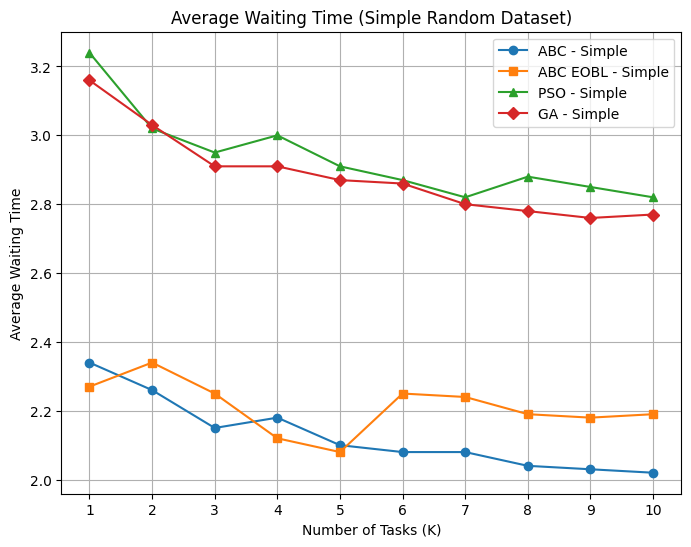
\includegraphics[width=0.75\linewidth]{gambar/Grafik Average Waiting Time Simple Random.png}
    \caption{Grafik \textit{average waiting time simple random}}
\end{figure}

\newpage

\begin{figure} [H]
    \centering
    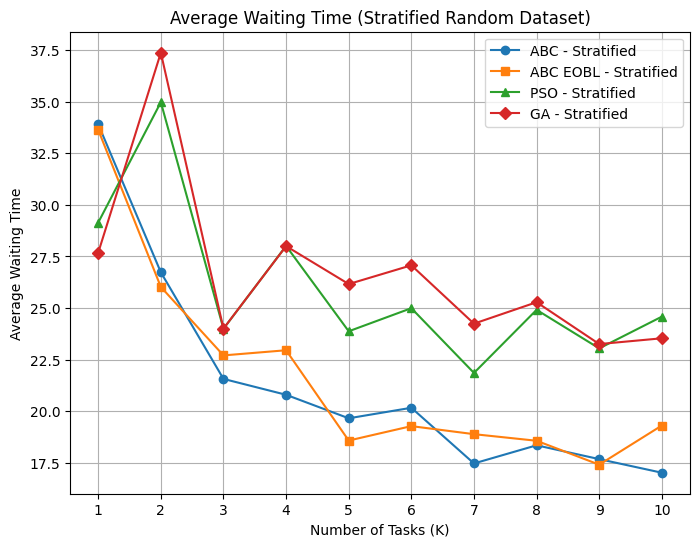
\includegraphics[width=0.75\linewidth]{gambar/Grafik Average Waiting Time Stratified Random.png}
    \caption{Grafik \textit{average waiting time stratified random}}
\end{figure}

\begin{figure} [H]
    \centering
    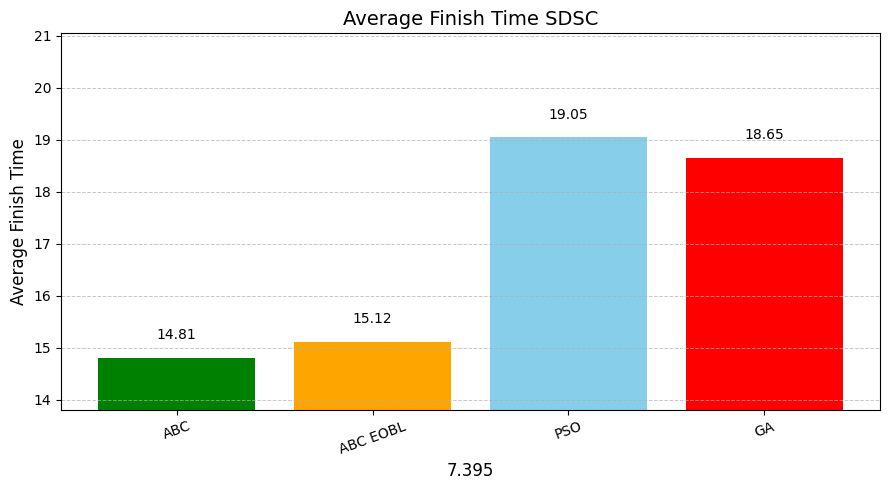
\includegraphics[width=0.75\linewidth]{gambar/Grafik Average Waiting Time SDSC.png}
    \caption{Grafik \textit{average waiting time} SDSC}
\end{figure}

\newpage

\begin{figure} [H]
    \centering
    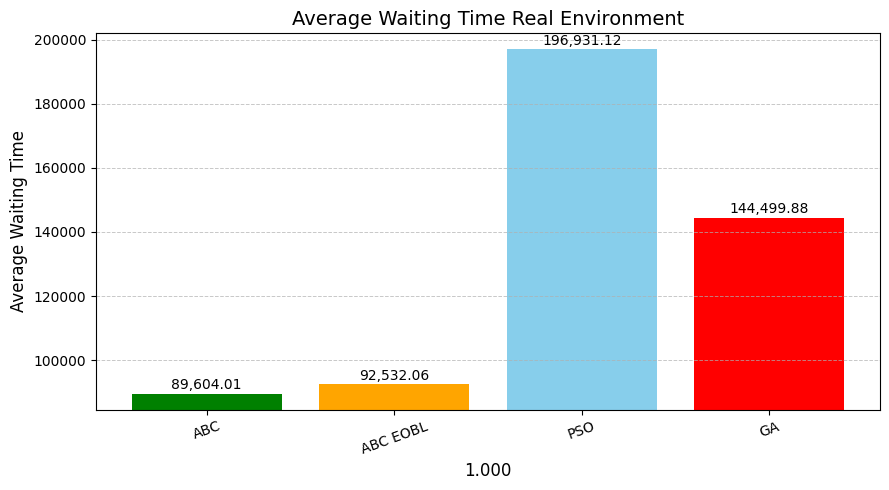
\includegraphics[width=0.75\linewidth]{gambar/Grafik Average Waiting Time Real Environment.png}
    \caption{Grafik \textit{average waiting rime real environment}}
\end{figure}

\subsection{\textit{Scheduling Length} (\textit{Lower Better})}
\textit{Scheduling length} adalah waktu keseluruhan yang diperlukan untuk menyelesaikan seluruh proses penjadwalan dan simulasi \textit{cloud} dari awal hingga akhir. Semakin rendah nilai \textit{scheduling length}, semakin efisien algoritma dalam menyelesaikan seluruh rangkaian tugas yang dijadwalkan.

\begin{table} [H]
\centering
\caption{\textit{Scheduling length simple random}}
\begin{tabular}{|>{\raggedleft\arraybackslash}m{0.12\linewidth}|
                >{\raggedleft\arraybackslash}m{0.17\linewidth}|
                >{\raggedleft\arraybackslash}m{0.17\linewidth}|
                >{\raggedleft\arraybackslash}m{0.17\linewidth}|
                >{\raggedleft\arraybackslash}m{0.17\linewidth}|}
\rowcolor{blue!30}
\hline
\multicolumn{1}{|>{\centering\arraybackslash}m{0.12\linewidth}|}{\textbf{\textit{Cloudlets}}} & 
\multicolumn{1}{>{\centering\arraybackslash}m{0.17\linewidth}|}{\textbf{ABC \textit{Simple}}} & 
\multicolumn{1}{>{\centering\arraybackslash}m{0.17\linewidth}|}{\textbf{ABC EOBL \textit{Simple}}} & 
\multicolumn{1}{>{\centering\arraybackslash}m{0.17\linewidth}|}{\textbf{PSO \textit{Simple}}} & 
\multicolumn{1}{>{\centering\arraybackslash}m{0.17\linewidth}|}{\textbf{GA \textit{Simple}}} \\
\hline
1.000 & 743.400,60 & 734.004,60 & 1.011.223,50 & 1.100.030,10 \\
\hline
2.000 & 2.989.205,70 & 3.005.431,80 & 4.134.511,50 & 4.558.990,20 \\
\hline
3.000 & 6.745.376,40 & 6.740.484,00 & 9.175.560,90 & 10.147.693,20 \\
\hline
4.000 & 11.933.167,20 & 11.876.727,30 & 16.558.460,70 & 18.159.654,30 \\
\hline
5.000 & 18.509.958,60 & 18.387.784,50 & 25.723.842,00 & 28.000.251,60 \\
\hline
6.000 & 26.735.547,30 & 27.615.263,10 & 37.210.486,20 & 40.730.730,90 \\
\hline
7.000 & 36.415.642,20 & 37.677.615,00 & 50.093.097,90 & 55.060.249,20 \\
\hline
8.000 & 47.840.731,80 & 49.259.633,10 & 66.351.669,00 & 72.416.049,00 \\
\hline
9.000 & 60.439.857,00 & 62.205.504,00 & 83.618.349,00 & 91.436.716,50 \\
\hline
10.000 & 74.268.742,20 & 76.738.122,60 & 103.356.471,30 & 113.210.187,00 \\
\hline
\textbf{AVG} & \textcolor{green}{28.662.162,90} & 29.424.057,00 & 39.723.367,20 & 43.482.055,20 \\
\hline
\end{tabular}
\end{table}

\newpage

\begin{table} [H]
\centering
\caption{\textit{Scheduling length stratified random}}
\begin{tabular}{|>{\raggedleft\arraybackslash}m{0.12\linewidth}|
                >{\raggedleft\arraybackslash}m{0.17\linewidth}|
                >{\raggedleft\arraybackslash}m{0.17\linewidth}|
                >{\raggedleft\arraybackslash}m{0.17\linewidth}|
                >{\raggedleft\arraybackslash}m{0.17\linewidth}|}
\rowcolor{blue!30}
\hline
\multicolumn{1}{|>{\centering\arraybackslash}m{0.12\linewidth}|}{\textbf{\textit{Cloudlets}}} & 
\multicolumn{1}{>{\centering\arraybackslash}m{0.17\linewidth}|}{\textbf{ABC \textit{Stratified}}} & 
\multicolumn{1}{>{\centering\arraybackslash}m{0.17\linewidth}|}{\textbf{ABC EOBL \textit{Stratified}}} & 
\multicolumn{1}{>{\centering\arraybackslash}m{0.17\linewidth}|}{\textbf{PSO \textit{Stratified}}} & 
\multicolumn{1}{>{\centering\arraybackslash}m{0.17\linewidth}|}{\textbf{GA \textit{Stratified}}} \\
\hline
1.000 & 4.676.353,80 & 4.827.151,00 & 5.532.900,90 & 5.773.783,20 \\
\hline
2.000 & 20.407.372,80 & 21.623.870,00 & 29.768.208,00 & 32.249.119,20 \\
\hline
3.000 & 44.439.721,80 & 44.605.081,00 & 58.344.773,10 & 61.841.587,20 \\
\hline
4.000 & 83.050.715,40 & 85.349.216,00 & 113.632.170,90 & 128.966.949,60 \\
\hline
5.000 & 125.130.030,00 & 130.802.522,00 & 166.917.843,60 & 187.339.596,00 \\
\hline
6.000 & 189.955.734,00 & 189.742.191,00 & 260.844.148,50 & 288.369.367,80 \\
\hline
7.000 & 249.796.277,70 & 256.844.061,00 & 326.360.551,20 & 358.762.533,00 \\
\hline
8.000 & 331.913.006,70 & 346.656.235,00 & 469.951.368,90 & 509.912.484,00 \\
\hline
9.000 & 421.099.836,00 & 422.904.804,00 & 558.509.244,90 & 615.035.871,60 \\
\hline
10.000 & 514.190.867,10 & 547.779.267,00 & 723.139.092,60 & 797.767.736,10 \\
\hline
\textbf{AVG} & \textcolor{green}{198.465.991,53} & 205.113.440,00 & 271.300.030,26 & 298.601.902,77 \\
\hline
\end{tabular}
\end{table}

\begin{table} [H]
\centering
\caption{\textit{Scheduling length} SDSC}
\begin{tabular}{|>{\raggedleft\arraybackslash}m{0.12\linewidth}|
                >{\raggedleft\arraybackslash}m{0.17\linewidth}|
                >{\raggedleft\arraybackslash}m{0.17\linewidth}|
                >{\raggedleft\arraybackslash}m{0.17\linewidth}|
                >{\raggedleft\arraybackslash}m{0.17\linewidth}|}
\rowcolor{blue!30}
\hline
\multicolumn{1}{|>{\centering\arraybackslash}m{0.12\linewidth}|}{\textbf{\textit{Cloudlets}}} & 
\multicolumn{1}{>{\centering\arraybackslash}m{0.17\linewidth}|}{\textbf{ABC SDSC}} & 
\multicolumn{1}{>{\centering\arraybackslash}m{0.17\linewidth}|}{\textbf{ABC EOBL SDSC}} & 
\multicolumn{1}{>{\centering\arraybackslash}m{0.17\linewidth}|}{\textbf{PSO SDSC}} & 
\multicolumn{1}{>{\centering\arraybackslash}m{0.17\linewidth}|}{\textbf{GA SDSC}} \\
\hline
7.395 & \textcolor{green}{206.619.378,00} & 211.418.069,10 & 279.421.667,03 & 308.094.796,50 \\
\hline
\end{tabular}
\end{table}

\begin{table} [H]
\centering
\caption{\textit{Scheduling length real environment}}
\begin{tabular}{|>{\raggedleft\arraybackslash}m{0.1\linewidth}|
                >{\raggedleft\arraybackslash}m{0.17\linewidth}|
                >{\raggedleft\arraybackslash}m{0.17\linewidth}|
                >{\raggedleft\arraybackslash}m{0.17\linewidth}|
                >{\raggedleft\arraybackslash}m{0.17\linewidth}|}
\rowcolor{blue!30}
\hline
\multicolumn{1}{|>{\centering\arraybackslash}m{0.1\linewidth}|}{\textbf{\textit{Task}}} & 
\multicolumn{1}{>{\centering\arraybackslash}m{0.17\linewidth}|}{\textbf{ABC RE}} & 
\multicolumn{1}{>{\centering\arraybackslash}m{0.17\linewidth}|}{\textbf{ABC EOBL RE}} & 
\multicolumn{1}{>{\centering\arraybackslash}m{0.17\linewidth}|}{\textbf{PSO RE}} & 
\multicolumn{1}{>{\centering\arraybackslash}m{0.17\linewidth}|}{\textbf{GA RE}} \\
\hline
1.000 & \textcolor{green}{89.783.921,80} & 101.247.810,46 & 197.276.296,00 & 144.789.121,00 \\
\hline
\end{tabular}
\end{table}

Berdasarkan hasil pengujian yang disajikan pada tabel dan grafik, algoritma \textit{Artificial Bee Colony} (ABC) secara konsisten menunjukkan nilai \textit{scheduling length} paling rendah pada seluruh \textit{dataset} yang diuji, baik pada \textit{simple random}, \textit{stratified random}, maupun SDSC. Hal ini menunjukkan bahwa ABC memiliki efisiensi tertinggi dalam menyelesaikan seluruh proses penjadwalan dengan waktu yang paling singkat.

Algoritma ABC dengan \textit{Elite Opposition-Based Learning} (EOBL) menempati posisi kedua, dengan nilai \textit{scheduling length} yang sedikit lebih tinggi dibandingkan ABC, namun tetap lebih baik dibandingkan dengan algoritma lain, seperti \textit{Particle Swarm Optimization} (PSO) dan \textit{Genetic Algorithm} (GA).

Penyebab utama rendahnya \textit{scheduling length} pada ABC adalah kesederhanaan dan efektivitas mekanisme penjadwalan yang digunakan, tanpa menambah kompleksitas komputasi seperti pada metode ABC-EOBL. Sementara itu, tambahan mekanisme adaptasi dan diversifikasi solusi pada ABC-EOBL memang meningkatkan kemampuan pencarian solusi, namun menimbulkan \textit{overhead} yang menyebabkan total waktu penjadwalan menjadi lebih panjang dibandingkan dengan ABC saja.

\newpage

\begin{figure} [H]
    \centering
    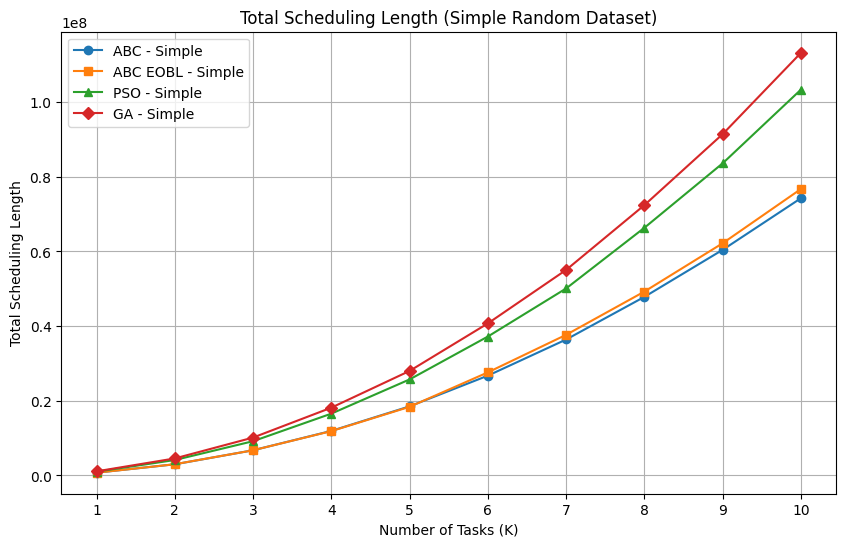
\includegraphics[width=0.75\linewidth]{gambar/Grafik Scheduling Length Simple Random.png}
    \caption{Grafik \textit{scheduling length simple random}}
\end{figure}

\begin{figure} [H]
    \centering
    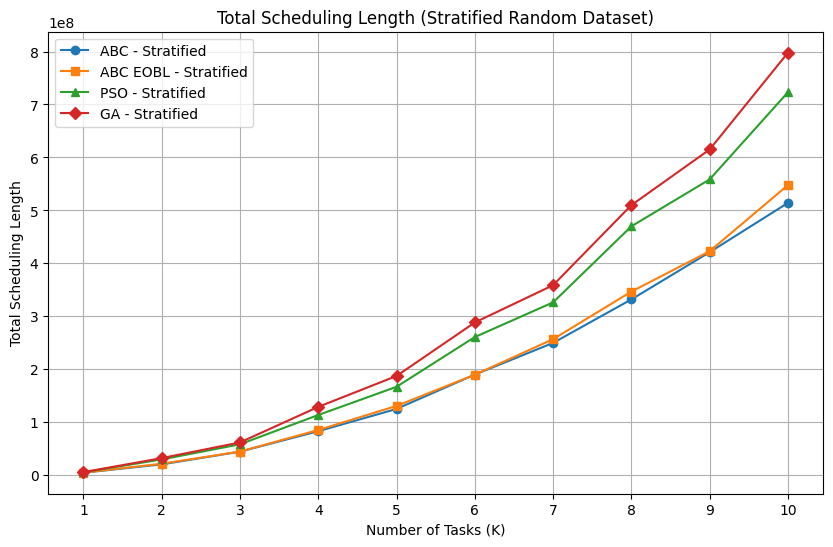
\includegraphics[width=0.75\linewidth]{gambar/Grafik Scheduling Length Stratified Random.png}
    \caption{Grafik \textit{scheduling length stratified random}}
\end{figure}

\newpage

\begin{figure} [H]
    \centering
    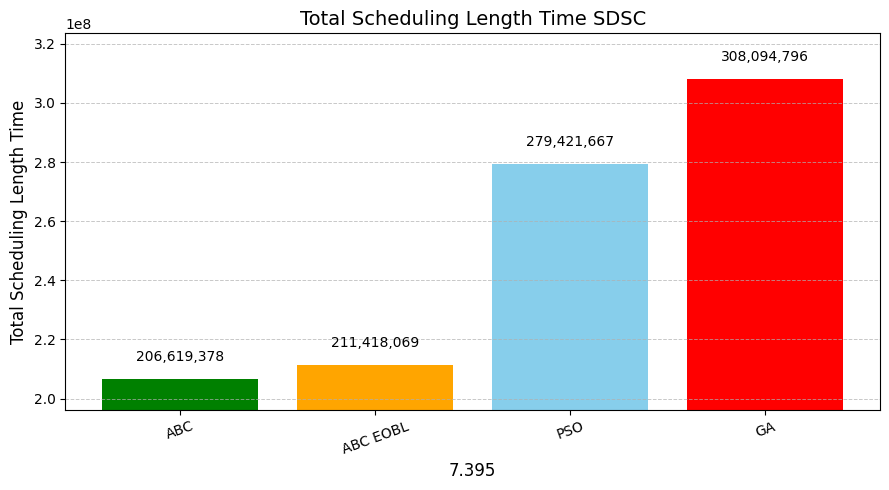
\includegraphics[width=0.75\linewidth]{gambar/Grafik Scheduling Length SDSC.png}
    \caption{Grafik \textit{scheduling length} SDSC}
\end{figure}

\begin{figure} [H]
    \centering
    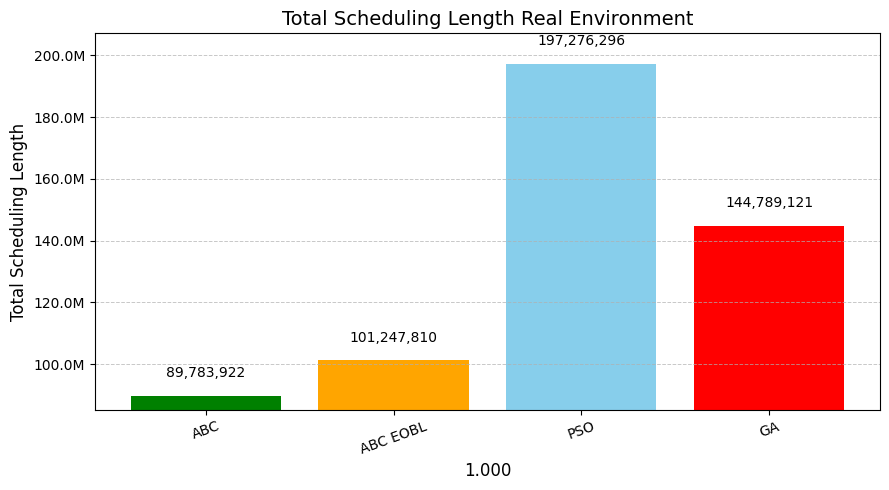
\includegraphics[width=0.75\linewidth]{gambar/Grafik Scheduling Length Real Environment.png}
    \caption{Grafik \textit{scheduling length real environment}}
\end{figure}

\subsection{\textit{Throughput} (\textit{Higher Better})}
\textit{Throughput} adalah jumlah tugas yang berhasil diselesaikan dalam satu unit waktu. Semakin tinggi nilai \textit{throughput}, semakin baik kinerja algoritma dalam menyelesaikan tugas secara efisien.

\newpage

\begin{table} [H]
\centering
\caption{\textit{Throughput simple random}}
\begin{tabular}{|>{\raggedleft\arraybackslash}m{0.12\linewidth}|
                >{\raggedleft\arraybackslash}m{0.17\linewidth}|
                >{\raggedleft\arraybackslash}m{0.17\linewidth}|
                >{\raggedleft\arraybackslash}m{0.17\linewidth}|
                >{\raggedleft\arraybackslash}m{0.17\linewidth}|}
\rowcolor{blue!30}
\hline
\multicolumn{1}{|>{\centering\arraybackslash}m{0.12\linewidth}|}{\textbf{\textit{Cloudlets}}} & 
\multicolumn{1}{>{\centering\arraybackslash}m{0.17\linewidth}|}{\textbf{ABC \textit{Simple}}} & 
\multicolumn{1}{>{\centering\arraybackslash}m{0.17\linewidth}|}{\textbf{ABC EOBL \textit{Simple}}} & 
\multicolumn{1}{>{\centering\arraybackslash}m{0.17\linewidth}|}{\textbf{PSO \textit{Simple}}} & 
\multicolumn{1}{>{\centering\arraybackslash}m{0.17\linewidth}|}{\textbf{GA \textit{Simple}}} \\
\hline
1.000 & 0,4164 & 0,4281 & 0,3060 & 0,3124 \\
\hline
2.000 & 0,4380 & 0,4249 & 0,3280 & 0,3272 \\
\hline
3.000 & 0,4603 & 0,4419 & 0,3370 & 0,3418 \\
\hline
4.000 & 0,4564 & 0,4698 & 0,3330 & 0,3426 \\
\hline
5.000 & 0,4753 & 0,4792 & 0,3430 & 0,3476 \\
\hline
6.000 & 0,4792 & 0,4435 & 0,3470 & 0,3483 \\
\hline
7.000 & 0,4803 & 0,4452 & 0,3540 & 0,3564 \\
\hline
8.000 & 0,4893 & 0,4548 & 0,3460 & 0,3587 \\
\hline
9.000 & 0,4920 & 0,4574 & 0,3500 & 0,3616 \\
\hline
10.000 & 0,4952 & 0,4547 & 0,3550 & 0,3601 \\
\hline
\textbf{AVG} & \textcolor{green}{0,4682} & 0,4500 & 0,3399 & 0,3457 \\
\hline
\end{tabular}
\end{table}

\begin{table} [H]
\centering
\caption{\textit{Throughput stratified random}}
\begin{tabular}{|>{\raggedleft\arraybackslash}m{0.12\linewidth}|
                >{\raggedleft\arraybackslash}m{0.17\linewidth}|
                >{\raggedleft\arraybackslash}m{0.17\linewidth}|
                >{\raggedleft\arraybackslash}m{0.17\linewidth}|
                >{\raggedleft\arraybackslash}m{0.17\linewidth}|}
\rowcolor{blue!30}
\hline
\multicolumn{1}{|>{\centering\arraybackslash}m{0.12\linewidth}|}{\textbf{\textit{Cloudlets}}} & 
\multicolumn{1}{>{\centering\arraybackslash}m{0.17\linewidth}|}{\textbf{ABC \textit{Stratified}}} & 
\multicolumn{1}{>{\centering\arraybackslash}m{0.17\linewidth}|}{\textbf{ABC EOBL \textit{Stratified}}} & 
\multicolumn{1}{>{\centering\arraybackslash}m{0.17\linewidth}|}{\textbf{PSO \textit{Stratified}}} & 
\multicolumn{1}{>{\centering\arraybackslash}m{0.17\linewidth}|}{\textbf{GA \textit{Stratified}}} \\
\hline
1.000 & 0,0282 & 0,0286 & 0,0336 & 0,0296 \\
\hline
2.000 & 0,0380 & 0,0379 & 0,0289 & 0,0271 \\
\hline
3.000 & 0,0466 & 0,0449 & 0,0421 & 0,0418 \\
\hline
4.000 & 0,0486 & 0,0442 & 0,0363 & 0,0361 \\
\hline
5.000 & 0,0518 & 0,0543 & 0,0423 & 0,0381 \\
\hline
6.000 & 0,0500 & 0,0517 & 0,0403 & 0,0369 \\
\hline
7.000 & 0,0575 & 0,0534 & 0,0450 & 0,0418 \\
\hline
8.000 & 0,0552 & 0,0544 & 0,0404 & 0,0395 \\
\hline
9.000 & 0,0570 & 0,0577 & 0,0435 & 0,0431 \\
\hline
10.000 & 0,0588 & 0,0523 & 0,0415 & 0,0426 \\
\hline
\textbf{AVG} & \textcolor{green}{0,0492} & 0,0479 & 0,0394 & 0,0377 \\
\hline
\end{tabular}
\end{table}

\begin{table} [H]
\centering
\caption{\textit{Throughput} SDSC}
\begin{tabular}{|>{\raggedleft\arraybackslash}m{0.12\linewidth}|
                >{\raggedleft\arraybackslash}m{0.15\linewidth}|
                >{\raggedleft\arraybackslash}m{0.25\linewidth}|
                >{\raggedleft\arraybackslash}m{0.15\linewidth}|
                >{\raggedleft\arraybackslash}m{0.15\linewidth}|}
\rowcolor{blue!30}
\hline
\multicolumn{1}{|>{\centering\arraybackslash}m{0.12\linewidth}|}{\textbf{\textit{Cloudlets}}} & 
\multicolumn{1}{>{\centering\arraybackslash}m{0.15\linewidth}|}{\textbf{ABC SDSC}} & 
\multicolumn{1}{>{\centering\arraybackslash}m{0.25\linewidth}|}{\textbf{ABC EOBL SDSC}} & 
\multicolumn{1}{>{\centering\arraybackslash}m{0.15\linewidth}|}{\textbf{PSO SDSC}} & 
\multicolumn{1}{>{\centering\arraybackslash}m{0.15\linewidth}|}{\textbf{GA SDSC}} \\
\hline
7.395 & \textcolor{green}{0,0674} & 0,0666 & 0,0526 & 0,0534 \\
\hline
\end{tabular}
\end{table}

\begin{table} [H]
\centering
\caption{\textit{Throughput real environment}}
\begin{tabular}{|>{\raggedleft\arraybackslash}m{0.1\linewidth}|
                >{\raggedleft\arraybackslash}m{0.17\linewidth}|
                >{\raggedleft\arraybackslash}m{0.17\linewidth}|
                >{\raggedleft\arraybackslash}m{0.17\linewidth}|
                >{\raggedleft\arraybackslash}m{0.17\linewidth}|}
\rowcolor{blue!30}
\hline
\multicolumn{1}{|>{\centering\arraybackslash}m{0.1\linewidth}|}{\textbf{\textit{Task}}} & 
\multicolumn{1}{>{\centering\arraybackslash}m{0.17\linewidth}|}{\textbf{ABC RE}} & 
\multicolumn{1}{>{\centering\arraybackslash}m{0.17\linewidth}|}{\textbf{ABC EOBL RE}} & 
\multicolumn{1}{>{\centering\arraybackslash}m{0.17\linewidth}|}{\textbf{PSO RE}} & 
\multicolumn{1}{>{\centering\arraybackslash}m{0.17\linewidth}|}{\textbf{GA RE}} \\
\hline
1.000 & \textcolor{green}{5,55} & 5,31 & 2,90 & 3,49 \\
\hline
\end{tabular}
\end{table}

Berdasarkan hasil pengujian yang disajikan pada tabel dan grafik, algoritma \textit{Artificial Bee Colony} (ABC) secara konsisten menunjukkan nilai \textit{throughput} tertinggi pada seluruh \textit{dataset} yang diuji, baik pada \textit{simple random}, \textit{stratified random}, maupun SDSC. Hal ini mengindikasikan bahwa ABC memiliki kapasitas penyelesaian tugas per satuan waktu yang paling optimal dibandingkan dengan algoritma lainnya.

Algoritma ABC dengan \textit{Elite Opposition-Based Learning} (EOBL) menempati posisi kedua, dengan nilai \textit{throughput} yang sedikit lebih rendah dibandingkan ABC, tetapi masih lebih tinggi daripada algoritma \textit{Particle Swarm Optimization} (PSO) dan \textit{Genetic Algorithm} (GA).

Keunggulan \textit{throughput} ABC ini disebabkan oleh mekanisme pencarian solusi yang efisien dan distribusi tugas yang optimal, memungkinkan penyelesaian lebih banyak tugas dalam waktu yang lebih singkat. Meskipun ABC-EOBL dirancang untuk memperbaiki pencarian solusi dengan menghindari jebakan lokal dan meningkatkan eksplorasi, proses ini mengarah pada evaluasi solusi lawan yang lebih banyak, yang berpotensi mengurangi efisiensi pencarian dan alokasi tugas dalam waktu singkat. Dengan kata lain, meskipun ABC-EOBL dapat memperbaiki kualitas solusi dengan memperluas ruang pencarian, proses pencarian yang lebih kompleks ini mengurangi kemampuan algoritma untuk menyelesaikan lebih banyak tugas dalam satuan waktu yang terbatas, sehingga menyebabkan penurunan nilai \textit{throughput} jika dibandingkan dengan ABC yang lebih efisien dalam distribusi tugas dan konvergensi solusi.

\begin{figure} [H]
    \centering
    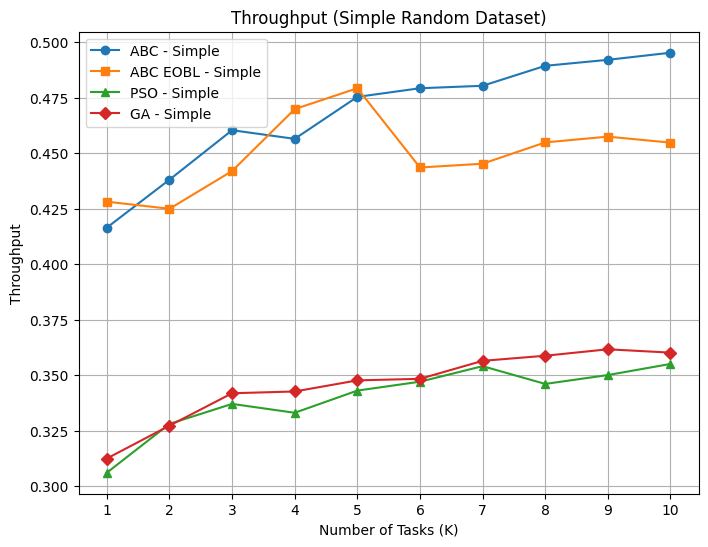
\includegraphics[width=0.75\linewidth]{gambar/Grafik Throughput Simple Random.png}
    \caption{Grafik \textit{throughput simple random}}
\end{figure}

\newpage

\begin{figure} [H]
    \centering
    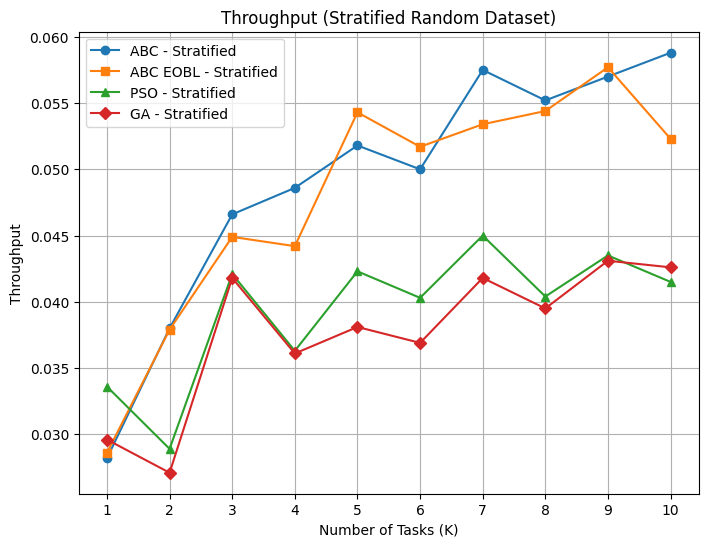
\includegraphics[width=0.75\linewidth]{gambar/Grafik Throughput Stratified Random.png}
    \caption{Grafik \textit{throughput stratified random}}
\end{figure}

\begin{figure} [H]
    \centering
    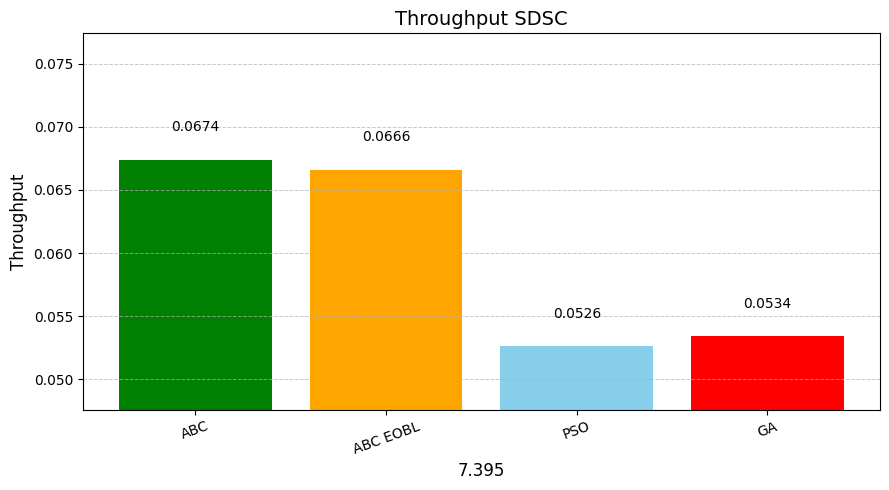
\includegraphics[width=0.75\linewidth]{gambar/Grafik Throughput SDSC.png}
    \caption{Grafik \textit{throughput} SDSC}
\end{figure}

\newpage

\begin{figure} [H]
    \centering
    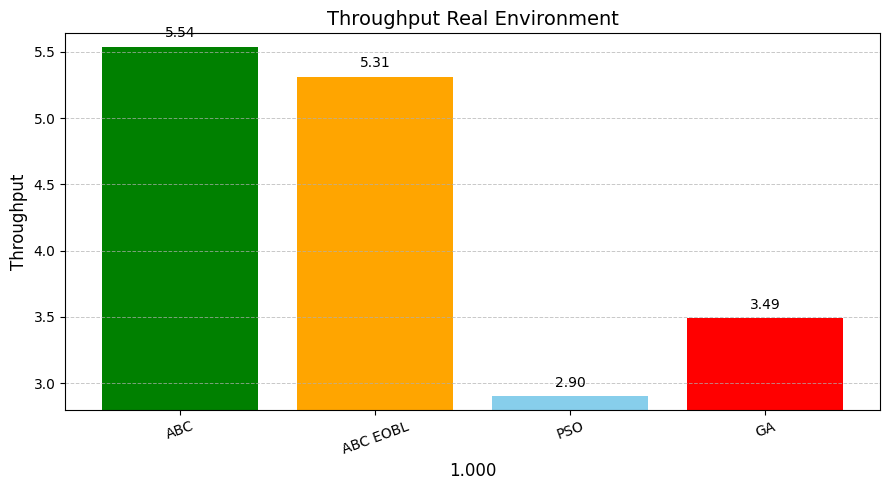
\includegraphics[width=0.75\linewidth]{gambar/Grafik Throughput Real Environment.png}
    \caption{Grafik \textit{throughput real environment}}
\end{figure}

\subsection{\textit{Resource Utilization} (\textit{Higher Better})}
\textit{Resource utilization} mengukur seberapa optimal sumber daya \textit{cloud} digunakan oleh algoritma dalam penjadwalan tugas. Semakin tinggi nilai \textit{resource utilization}, semakin efisien algoritma dalam memanfaatkan sumber daya yang tersedia.

\begin{table} [H]
\centering
\caption{\textit{Resource utilization simple random}}
\begin{tabular}{|>{\raggedleft\arraybackslash}m{0.12\linewidth}|
                >{\raggedleft\arraybackslash}m{0.17\linewidth}|
                >{\raggedleft\arraybackslash}m{0.17\linewidth}|
                >{\raggedleft\arraybackslash}m{0.17\linewidth}|
                >{\raggedleft\arraybackslash}m{0.17\linewidth}|}
\rowcolor{blue!30}
\hline
\multicolumn{1}{|>{\centering\arraybackslash}m{0.12\linewidth}|}{\textbf{\textit{Cloudlets}}} & 
\multicolumn{1}{>{\centering\arraybackslash}m{0.17\linewidth}|}{\textbf{ABC \textit{Simple}}} & 
\multicolumn{1}{>{\centering\arraybackslash}m{0.17\linewidth}|}{\textbf{ABC EOBL \textit{Simple}}} & 
\multicolumn{1}{>{\centering\arraybackslash}m{0.17\linewidth}|}{\textbf{PSO \textit{Simple}}} & 
\multicolumn{1}{>{\centering\arraybackslash}m{0.17\linewidth}|}{\textbf{GA \textit{Simple}}} \\
\hline
1.000 & 46,19 & 47,69 & 32,58 & 32,76 \\
\hline
2.000 & 48,42 & 47,05 & 34,73 & 34,05 \\
\hline
3.000 & 51,14 & 49,10 & 35,76 & 35,76 \\
\hline
4.000 & 50,39 & 51,98 & 35,14 & 35,58 \\
\hline
5.000 & 52,50 & 52,99 & 36,20 & 36,13 \\
\hline
6.000 & 52,99 & 48,83 & 36,61 & 36,20 \\
\hline
7.000 & 53,17 & 49,06 & 37,45 & 37,13 \\
\hline
8.000 & 54,20 & 50,19 & 36,63 & 37,39 \\
\hline
9.000 & 54,50 & 50,50 & 37,00 & 37,69 \\
\hline
10.000 & 54,82 & 50,09 & 37,45 & 37,46 \\
\hline
\textbf{AVG} & \textcolor{green}{51,83} & 49,75 & 35,96 & 36,02 \\
\hline
\end{tabular}
\end{table}

\newpage

\begin{table} [H]
\centering
\caption{\textit{Resource utilization stratified random}}
\begin{tabular}{|>{\raggedleft\arraybackslash}m{0.12\linewidth}|
                >{\raggedleft\arraybackslash}m{0.17\linewidth}|
                >{\raggedleft\arraybackslash}m{0.17\linewidth}|
                >{\raggedleft\arraybackslash}m{0.17\linewidth}|
                >{\raggedleft\arraybackslash}m{0.17\linewidth}|}
\rowcolor{blue!30}
\hline
\multicolumn{1}{|>{\centering\arraybackslash}m{0.12\linewidth}|}{\textbf{\textit{Cloudlets}}} & 
\multicolumn{1}{>{\centering\arraybackslash}m{0.17\linewidth}|}{\textbf{ABC \textit{Stratified}}} & 
\multicolumn{1}{>{\centering\arraybackslash}m{0.17\linewidth}|}{\textbf{ABC EOBL \textit{Stratified}}} & 
\multicolumn{1}{>{\centering\arraybackslash}m{0.17\linewidth}|}{\textbf{PSO \textit{Stratified}}} & 
\multicolumn{1}{>{\centering\arraybackslash}m{0.17\linewidth}|}{\textbf{GA \textit{Stratified}}} \\
\hline
1.000 & 25,51 & 25,32 & 29,23 & 25,84 \\
\hline
2.000 & 32,64 & 32,12 & 23,36 & 21,60 \\
\hline
3.000 & 40,93 & 39,73 & 35,71 & 34,94 \\
\hline
4.000 & 41,69 & 37,76 & 29,48 & 28,77 \\
\hline
5.000 & 45,15 & 47,15 & 35,42 & 31,18 \\
\hline
6.000 & 42,85 & 44,19 & 32,76 & 29,36 \\
\hline
7.000 & 49,82 & 46,13 & 37,36 & 34,04 \\
\hline
8.000 & 47,43 & 46,69 & 32,92 & 31,55 \\
\hline
9.000 & 49,16 & 49,94 & 35,97 & 34,98 \\
\hline
10.000 & 50,40 & 44,47 & 33,68 & 33,91 \\
\hline
\textbf{AVG} & \textcolor{green}{42,56} & 41,35 & 32,59 & 30,62 \\
\hline
\end{tabular}
\end{table}

\begin{table} [H]
\centering
\caption{\textit{Resource utilization} SDSC}
\begin{tabular}{|>{\raggedleft\arraybackslash}m{0.12\linewidth}|
                >{\raggedleft\arraybackslash}m{0.15\linewidth}|
                >{\raggedleft\arraybackslash}m{0.25\linewidth}|
                >{\raggedleft\arraybackslash}m{0.15\linewidth}|
                >{\raggedleft\arraybackslash}m{0.15\linewidth}|}
\rowcolor{blue!30}
\hline
\multicolumn{1}{|>{\centering\arraybackslash}m{0.12\linewidth}|}{\textbf{\textit{Cloudlets}}} & 
\multicolumn{1}{>{\centering\arraybackslash}m{0.15\linewidth}|}{\textbf{ABC SDSC}} & 
\multicolumn{1}{>{\centering\arraybackslash}m{0.25\linewidth}|}{\textbf{ABC EOBL SDSC}} & 
\multicolumn{1}{>{\centering\arraybackslash}m{0.15\linewidth}|}{\textbf{PSO SDSC}} & 
\multicolumn{1}{>{\centering\arraybackslash}m{0.15\linewidth}|}{\textbf{GA SDSC}} \\
\hline
7.395 & \textcolor{green}{43,94} & 43,27 & 32,69 & 32,19 \\
\hline
\end{tabular}
\end{table}

\begin{table} [H]
\centering
\caption{\textit{Resource utilization real environment}}
\begin{tabular}{|>{\raggedleft\arraybackslash}m{0.1\linewidth}|
                >{\raggedleft\arraybackslash}m{0.17\linewidth}|
                >{\raggedleft\arraybackslash}m{0.17\linewidth}|
                >{\raggedleft\arraybackslash}m{0.17\linewidth}|
                >{\raggedleft\arraybackslash}m{0.17\linewidth}|}
\rowcolor{blue!30}
\hline
\multicolumn{1}{|>{\centering\arraybackslash}m{0.1\linewidth}|}{\textbf{\textit{Task}}} & 
\multicolumn{1}{>{\centering\arraybackslash}m{0.17\linewidth}|}{\textbf{ABC RE}} & 
\multicolumn{1}{>{\centering\arraybackslash}m{0.17\linewidth}|}{\textbf{ABC EOBL RE}} & 
\multicolumn{1}{>{\centering\arraybackslash}m{0.17\linewidth}|}{\textbf{PSO RE}} & 
\multicolumn{1}{>{\centering\arraybackslash}m{0.17\linewidth}|}{\textbf{GA RE}} \\
\hline
1.000 & \textcolor{green}{16,97} & 16,59 & 15,94 & 15,31 \\
\hline
\end{tabular}
\end{table}

Berdasarkan hasil pengujian yang disajikan pada tabel dan grafik, algoritma \textit{Artificial Bee Colony} (ABC) menunjukkan pemanfaatan sumber daya tertinggi pada seluruh \textit{dataset} yang diuji, baik pada \textit{simple random}, \textit{stratified random}, maupun SDSC. Hal ini menunjukkan bahwa ABC mampu mengalokasikan sumber daya secara lebih optimal dibandingkan dengan algoritma lainnya.

Algoritma ABC dengan \textit{Elite Opposition-Based Learning} (EOBL) menempati posisi kedua, dengan pemanfaatan yang sedikit lebih rendah dibandingkan ABC, namun masih lebih tinggi daripada \textit{Particle Swarm Optimization} (PSO) dan \textit{Genetic Algorithm} (GA).

Penurunan pemanfaatan sumber daya pada ABC-EOBL disebabkan oleh kompleksitas tambahan dari mekanisme EOBL, yang melibatkan evaluasi solusi lawan yang lebih banyak. Meskipun EOBL bertujuan untuk memperbaiki pencarian solusi dan menghindari jebakan lokal, proses ini membutuhkan lebih banyak waktu komputasi untuk memproses dan mengevaluasi solusi yang lebih banyak. Dengan meningkatnya jumlah solusi yang harus dievaluasi, waktu komputasi yang dibutuhkan menjadi lebih lama, sehingga menyebabkan alokasi sumber daya yang lebih banyak terbuang pada proses evaluasi dan seleksi, bukan pada penyelesaian tugas yang efektif. Akibatnya, alokasi sumber daya menjadi kurang optimal dibandingkan dengan algoritma ABC yang lebih sederhana dan efisien dalam distribusi tugas.

\newpage

\begin{figure} [H]
    \centering
    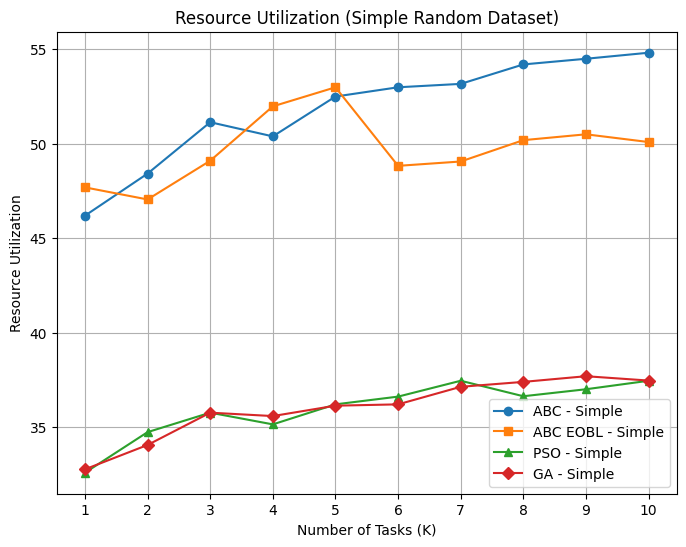
\includegraphics[width=0.75\linewidth]{gambar/Grafik Resource Utilization Simple Random.png}
    \caption{Grafik \textit{resource utilization simple random}}
\end{figure}

\begin{figure} [H]
    \centering
    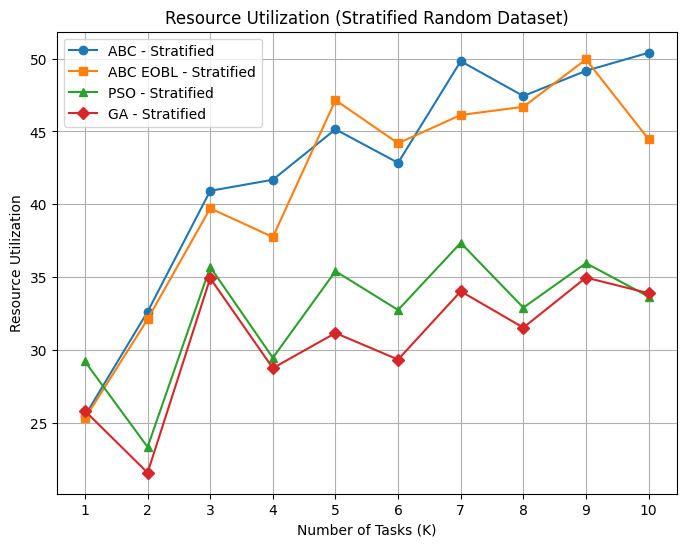
\includegraphics[width=0.75\linewidth]{gambar/Grafik Resource Utilization Stratified Random.png}
    \caption{Grafik \textit{resource utilization stratified random}}
\end{figure}

\newpage

\begin{figure} [H]
    \centering
    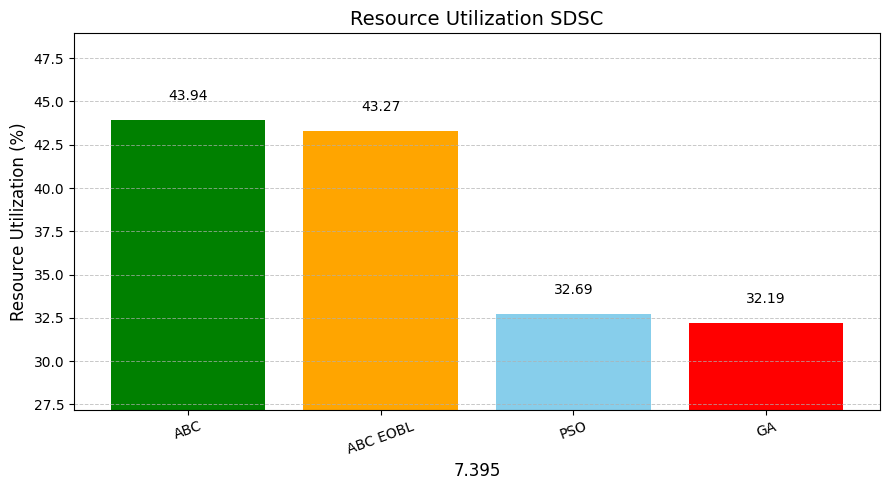
\includegraphics[width=0.75\linewidth]{gambar/Grafik Resource Utilization SDSC.png}
    \caption{Grafik \textit{resource utilization} SDSC}
\end{figure}

\begin{figure} [H]
    \centering
    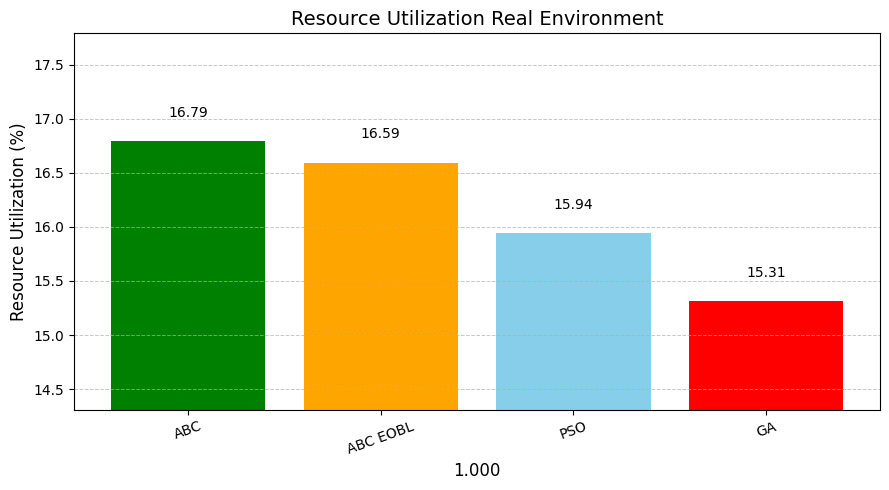
\includegraphics[width=0.75\linewidth]{gambar/Grafik Resource Utilization Real Environment.png}
    \caption{Grafik \textit{resource utilization real environment}}
\end{figure}

\subsection{\textit{Total Energy Consumption} (\textit{Lower Better})}
\textit{Total energy consumption} mengukur tingkat penggunaan energi yang dibutuhkan oleh semua sumber daya \textit{cloud}. Semakin rendah nilai dari parameter ini, semakin efisien algoritma dalam memanfaatkan energi, yang menunjukkan kinerja yang lebih baik.

\newpage

\begin{table} [H]
\centering
\caption{\textit{Total energy consumption simple random}}
\begin{tabular}{|>{\raggedleft\arraybackslash}m{0.12\linewidth}|
                >{\raggedleft\arraybackslash}m{0.17\linewidth}|
                >{\raggedleft\arraybackslash}m{0.17\linewidth}|
                >{\raggedleft\arraybackslash}m{0.17\linewidth}|
                >{\raggedleft\arraybackslash}m{0.17\linewidth}|}
\rowcolor{blue!30}
\hline
\multicolumn{1}{|>{\centering\arraybackslash}m{0.12\linewidth}|}{\textbf{\textit{Cloudlets}}} & 
\multicolumn{1}{>{\centering\arraybackslash}m{0.17\linewidth}|}{\textbf{ABC \textit{Simple}}} & 
\multicolumn{1}{>{\centering\arraybackslash}m{0.17\linewidth}|}{\textbf{ABC EOBL \textit{Simple}}} & 
\multicolumn{1}{>{\centering\arraybackslash}m{0.17\linewidth}|}{\textbf{PSO \textit{Simple}}} & 
\multicolumn{1}{>{\centering\arraybackslash}m{0.17\linewidth}|}{\textbf{GA \textit{Simple}}} \\
\hline
1.000 & 12,52 & 11,48 & 15,33 & 15,73 \\
\hline
2.000 & 20,45 & 23,04 & 30,07 & 30,88 \\
\hline
3.000 & 27,87 & 33,64 & 43,81 & 45,20 \\
\hline
4.000 & 38,33 & 43,61 & 59,17 & 60,46 \\
\hline
5.000 & 42,13 & 53,47 & 73,21 & 73,89 \\
\hline
6.000 & 53,22 & 68,83 & 88,15 & 89,40 \\
\hline
7.000 & 59,62 & 80,70 & 101,62 & 102,90 \\
\hline
8.000 & 68,75 & 91,68 & 118,04 & 117,50 \\
\hline
9.000 & 73,15 & 102,68 & 132,60 & 131,59 \\
\hline
10.000 & 90,62 & 114,18 & 145,75 & 146,19 \\
\hline
\textbf{AVG} & \textcolor{green}{48,67} & 62,33 & 80,78 & 81,37 \\
\hline
\end{tabular}
\end{table}

\begin{table} [H]
\centering
\caption{\textit{Total energy consumption stratified random}}
\begin{tabular}{|>{\raggedleft\arraybackslash}m{0.12\linewidth}|
                >{\raggedleft\arraybackslash}m{0.17\linewidth}|
                >{\raggedleft\arraybackslash}m{0.17\linewidth}|
                >{\raggedleft\arraybackslash}m{0.17\linewidth}|
                >{\raggedleft\arraybackslash}m{0.17\linewidth}|}
\rowcolor{blue!30}
\hline
\multicolumn{1}{|>{\centering\arraybackslash}m{0.12\linewidth}|}{\textbf{\textit{Cloudlets}}} & 
\multicolumn{1}{>{\centering\arraybackslash}m{0.17\linewidth}|}{\textbf{ABC \textit{Stratified}}} & 
\multicolumn{1}{>{\centering\arraybackslash}m{0.17\linewidth}|}{\textbf{ABC EOBL \textit{Stratified}}} & 
\multicolumn{1}{>{\centering\arraybackslash}m{0.17\linewidth}|}{\textbf{PSO \textit{Stratified}}} & 
\multicolumn{1}{>{\centering\arraybackslash}m{0.17\linewidth}|}{\textbf{GA \textit{Stratified}}} \\
\hline
1.000 & 130,93 & 125,19 & 125,80 & 122,14 \\
\hline
2.000 & 195,26 & 204,49 & 260,78 & 269,33 \\
\hline
3.000 & 279,38 & 278,69 & 315,51 & 315,64 \\
\hline
4.000 & 362,91 & 383,29 & 479,57 & 479,46 \\
\hline
5.000 & 420,67 & 421,32 & 535,27 & 560,04 \\
\hline
6.000 & 527,21 & 532,18 & 696,44 & 722,26 \\
\hline
7.000 & 563,93 & 596,23 & 711,64 & 758,35 \\
\hline
8.000 & 675,69 & 687,52 & 907,06 & 949,97 \\
\hline
9.000 & 739,10 & 731,50 & 952,50 & 993,14 \\
\hline
10.000 & 809,38 & 906,22 & 1.108,87 & 1.143,16 \\
\hline
\textbf{AVG} & \textcolor{green}{470,45} & 486,66 & 609,34 & 631,35 \\
\hline
\end{tabular}
\end{table}

\begin{table} [H]
\centering
\caption{\textit{Total energy consumption} SDSC}
\begin{tabular}{|>{\raggedleft\arraybackslash}m{0.12\linewidth}|
                >{\raggedleft\arraybackslash}m{0.15\linewidth}|
                >{\raggedleft\arraybackslash}m{0.25\linewidth}|
                >{\raggedleft\arraybackslash}m{0.15\linewidth}|
                >{\raggedleft\arraybackslash}m{0.15\linewidth}|}
\rowcolor{blue!30}
\hline
\multicolumn{1}{|>{\centering\arraybackslash}m{0.12\linewidth}|}{\textbf{\textit{Cloudlets}}} & 
\multicolumn{1}{>{\centering\arraybackslash}m{0.15\linewidth}|}{\textbf{ABC SDSC}} & 
\multicolumn{1}{>{\centering\arraybackslash}m{0.25\linewidth}|}{\textbf{ABC EOBL SDSC}} & 
\multicolumn{1}{>{\centering\arraybackslash}m{0.15\linewidth}|}{\textbf{PSO SDSC}} & 
\multicolumn{1}{>{\centering\arraybackslash}m{0.15\linewidth}|}{\textbf{GA SDSC}} \\
\hline
7.395 & \textcolor{green}{497,37} & 498,76 & 613,34 & 656,95 \\
\hline
\end{tabular}
\end{table}

Berdasarkan hasil pengujian yang disajikan pada tabel dan grafik, algoritma ABC menunjukkan konsumsi energi paling rendah pada seluruh \textit{dataset} yang diuji, baik pada \textit{simple random}, \textit{stratified random}, maupun SDSC. Ini menunjukkan bahwa ABC sangat efisien dalam memanfaatkan energi dibandingkan dengan algoritma lainnya.

Algoritma ABC dengan \textit{Elite Opposition-Based Learning} (EOBL) menempati posisi kedua, dengan konsumsi energi yang sedikit lebih tinggi dibandingkan ABC, namun tetap lebih baik dibandingkan dengan \textit{Particle Swarm Optimization} (PSO) dan \textit{Genetic Algorithm} (GA). Pada \textit{dataset} SDSC, selisih konsumsi energi antara ABC dan ABC-EOBL sangat kecil, yang menunjukkan bahwa meskipun penambahan strategi EOBL pada ABC memberikan sedikit peningkatan dalam efisiensi, ABC tetap menjadi pilihan terbaik dalam hal penghematan energi.

Peningkatan konsumsi energi pada algoritma ABC-EOBL disebabkan oleh tambahan kompleksitas dari proses evaluasi solusi lawan yang dilakukan oleh metode EOBL. Setiap evaluasi solusi lawan memerlukan lebih banyak perhitungan dan proses komputasi, yang berimbas pada penggunaan daya yang lebih tinggi. Meskipun EOBL bertujuan untuk memperbaiki pencarian solusi dan menghindari jebakan lokal, kompleksitas tambahan ini menyebabkan peningkatan waktu komputasi dan konsumsi energi yang lebih besar dibandingkan dengan algoritma ABC yang lebih sederhana dan langsung dalam alokasi tugas.

\begin{figure} [H]
    \centering
    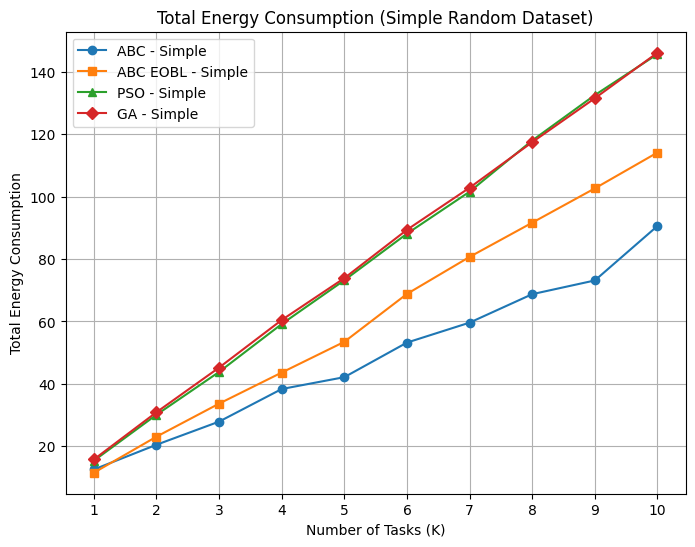
\includegraphics[width=0.75\linewidth]{gambar/Grafik Total Energy Consumption Simple Random.png}
    \caption{Grafik \textit{total energy consumption simple random}}
\end{figure}

\newpage

\begin{figure} [H]
    \centering
    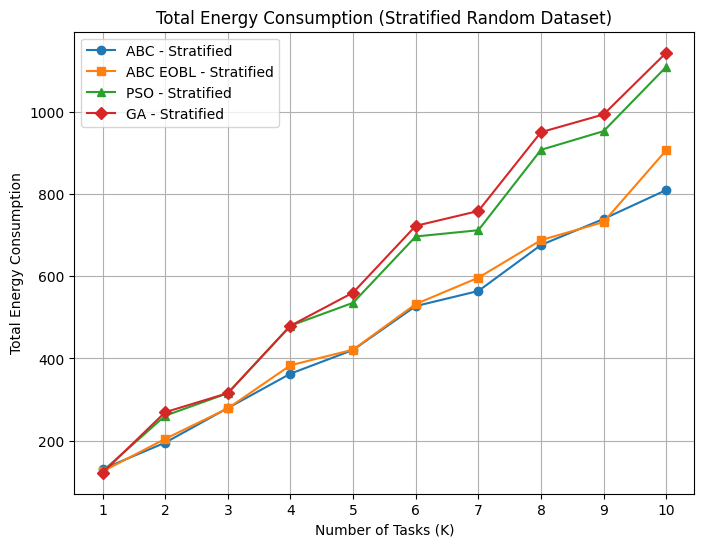
\includegraphics[width=0.75\linewidth]{gambar/Grafik Total Energy Consumption Stratified Random.png}
    \caption{Grafik \textit{total energy consumption stratified random}}
\end{figure}

\begin{figure} [H]
    \centering
    \includegraphics[width=0.75\linewidth]{gambar/Grafik Total Energy Consumption SDSC.png}
    \caption{Grafik \textit{total energy consumption} SDSC}
\end{figure}

\subsection{\textit{Imbalance Degree} (\textit{Lower Better})}
\textit{Imbalance degree} mengukur ketidakseimbangan dalam durasi pemrosesan tugas. Semakin rendah nilai \textit{imbalance degree}, semakin baik kinerja algoritma dalam mendistribusikan beban tugas secara merata, yang berarti durasi pemrosesan antar tugas lebih seimbang.

\newpage

\begin{table} [H]
\centering
\caption{\textit{Imbalance degree simple random}}
\begin{tabular}{|>{\raggedleft\arraybackslash}m{0.12\linewidth}|
                >{\raggedleft\arraybackslash}m{0.17\linewidth}|
                >{\raggedleft\arraybackslash}m{0.17\linewidth}|
                >{\raggedleft\arraybackslash}m{0.17\linewidth}|
                >{\raggedleft\arraybackslash}m{0.17\linewidth}|}
\rowcolor{blue!30}
\hline
\multicolumn{1}{|>{\centering\arraybackslash}m{0.12\linewidth}|}{\textbf{\textit{Cloudlets}}} & 
\multicolumn{1}{>{\centering\arraybackslash}m{0.17\linewidth}|}{\textbf{ABC \textit{Simple}}} & 
\multicolumn{1}{>{\centering\arraybackslash}m{0.17\linewidth}|}{\textbf{ABC EOBL \textit{Simple}}} & 
\multicolumn{1}{>{\centering\arraybackslash}m{0.17\linewidth}|}{\textbf{PSO \textit{Simple}}} & 
\multicolumn{1}{>{\centering\arraybackslash}m{0.17\linewidth}|}{\textbf{GA \textit{Simple}}} \\
\hline
1.000 & 1,80 & 1,80 & 1,88 & 1,89 \\
\hline
2.000 & 1,81 & 1,80 & 1,89 & 1,86 \\
\hline
3.000 & 1,80 & 1,80 & 1,88 & 1,91 \\
\hline
4.000 & 1,81 & 1,80 & 1,90 & 1,91 \\
\hline
5.000 & 1,81 & 1,80 & 1,90 & 1,92 \\
\hline
6.000 & 1,81 & 1,81 & 1,90 & 1,92 \\
\hline
7.000 & 1,81 & 1,81 & 1,89 & 1,92 \\
\hline
8.000 & 1,81 & 1,81 & 1,89 & 1,92 \\
\hline
9.000 & 1,81 & 1,81 & 1,89 & 1,92 \\
\hline
10.000 & 1,81 & 1,81 & 1,89 & 1,92 \\
\hline
\textbf{AVG} & 1,808 & \textcolor{green}{1,805} & 1,891 & 1,909 \\
\hline
\end{tabular}
\end{table}

\begin{table} [H]
\centering
\caption{\textit{Imbalance degree stratified random}}
\begin{tabular}{|>{\raggedleft\arraybackslash}m{0.12\linewidth}|
                >{\raggedleft\arraybackslash}m{0.17\linewidth}|
                >{\raggedleft\arraybackslash}m{0.17\linewidth}|
                >{\raggedleft\arraybackslash}m{0.17\linewidth}|
                >{\raggedleft\arraybackslash}m{0.17\linewidth}|}
\rowcolor{blue!30}
\hline
\multicolumn{1}{|>{\centering\arraybackslash}m{0.12\linewidth}|}{\textbf{\textit{Cloudlets}}} & 
\multicolumn{1}{>{\centering\arraybackslash}m{0.17\linewidth}|}{\textbf{ABC \textit{Stratified}}} & 
\multicolumn{1}{>{\centering\arraybackslash}m{0.17\linewidth}|}{\textbf{ABC EOBL \textit{Stratified}}} & 
\multicolumn{1}{>{\centering\arraybackslash}m{0.17\linewidth}|}{\textbf{PSO \textit{Stratified}}} & 
\multicolumn{1}{>{\centering\arraybackslash}m{0.17\linewidth}|}{\textbf{GA \textit{Stratified}}} \\
\hline
1.000 & 41,25 & 35,91 & 42,12 & 43,40 \\
\hline
2.000 & 44,90 & 42,23 & 49,72 & 48,72 \\
\hline
3.000 & 45,47 & 44,18 & 47,53 & 47,02 \\
\hline
4.000 & 46,14 & 43,13 & 48,75 & 49,94 \\
\hline
5.000 & 46,41 & 45,99 & 48,47 & 49,68 \\
\hline
6.000 & 47,01 & 46,90 & 48,80 & 50,67 \\
\hline
7.000 & 46,86 & 46,46 & 48,94 & 49,34 \\
\hline
8.000 & 47,23 & 47,03 & 49,77 & 50,78 \\
\hline
9.000 & 46,74 & 46,60 & 48,87 & 50,08 \\
\hline
10.000 & 47,43 & 47,01 & 50,08 & 51,01 \\
\hline
\textbf{AVG} & 45,94 & \textcolor{green}{44,54} & 48,31 & 49,06 \\
\hline
\end{tabular}
\end{table}

\begin{table} [H]
\centering
\caption{\textit{Imbalance degree} SDSC}
\begin{tabular}{|>{\raggedleft\arraybackslash}m{0.12\linewidth}|
                >{\raggedleft\arraybackslash}m{0.15\linewidth}|
                >{\raggedleft\arraybackslash}m{0.25\linewidth}|
                >{\raggedleft\arraybackslash}m{0.15\linewidth}|
                >{\raggedleft\arraybackslash}m{0.15\linewidth}|}
\rowcolor{blue!30}
\hline
\multicolumn{1}{|>{\centering\arraybackslash}m{0.12\linewidth}|}{\textbf{\textit{Cloudlets}}} & 
\multicolumn{1}{>{\centering\arraybackslash}m{0.15\linewidth}|}{\textbf{ABC SDSC}} & 
\multicolumn{1}{>{\centering\arraybackslash}m{0.25\linewidth}|}{\textbf{ABC EOBL SDSC}} & 
\multicolumn{1}{>{\centering\arraybackslash}m{0.15\linewidth}|}{\textbf{PSO SDSC}} & 
\multicolumn{1}{>{\centering\arraybackslash}m{0.15\linewidth}|}{\textbf{GA SDSC}} \\
\hline
7.395 & 56,01 & \textcolor{green}{54,78} & 56,88 & 56,83 \\
\hline
\end{tabular}
\end{table}

\begin{table} [H]
\centering
\caption{\textit{Imbalance degree real environment}}
\begin{tabular}{|>{\raggedleft\arraybackslash}m{0.1\linewidth}|
                >{\raggedleft\arraybackslash}m{0.17\linewidth}|
                >{\raggedleft\arraybackslash}m{0.17\linewidth}|
                >{\raggedleft\arraybackslash}m{0.17\linewidth}|
                >{\raggedleft\arraybackslash}m{0.17\linewidth}|}
\rowcolor{blue!30}
\hline
\multicolumn{1}{|>{\centering\arraybackslash}m{0.1\linewidth}|}{\textbf{\textit{Task}}} & 
\multicolumn{1}{>{\centering\arraybackslash}m{0.17\linewidth}|}{\textbf{ABC RE}} & 
\multicolumn{1}{>{\centering\arraybackslash}m{0.17\linewidth}|}{\textbf{ABC EOBL RE}} & 
\multicolumn{1}{>{\centering\arraybackslash}m{0.17\linewidth}|}{\textbf{PSO RE}} & 
\multicolumn{1}{>{\centering\arraybackslash}m{0.17\linewidth}|}{\textbf{GA RE}} \\
\hline
1.000 & 0,334 & \textcolor{green}{0,246} & 1,395 & 0,861 \\
\hline
\end{tabular}
\end{table}

\newpage

Berdasarkan hasil pengujian yang disajikan pada tabel dan grafik eksperimen, algoritma \textit{Artificial Bee Colony} (ABC) yang diintegrasikan dengan \textit{Elite Opposition-Based Learning} menunjukkan \textit{imbalance degree} terendah dibandingkan dengan ABC, PSO, dan GA. Hal ini menunjukkan bahwa integrasi EOBL memungkinkan distribusi tugas yang lebih merata dan seimbang, karena mekanisme EOBL membantu menghindari jebakan lokal dan memperluas eksplorasi solusi yang lebih optimal.

Pada \textit{dataset simple random} dan \textit{stratified random}, ABC-EOBL juga menunjukkan nilai \textit{imbalance degree} yang lebih rendah dibandingkan dengan algoritma lainnya. Ini menandakan bahwa algoritma ABC-EOBL lebih efektif dalam distribusi beban tugas, berkat kemampuan EOBL dalam menjaga keseimbangan durasi pemrosesan tugas. Pendekatan ini mencegah ketidakseimbangan beban kerja antar tugas, mengoptimalkan pemanfaatan sumber daya, dan meningkatkan efisiensi secara keseluruhan.

Secara keseluruhan, integrasi EOBL pada ABC meningkatkan kemampuan algoritma untuk mengeksplorasi solusi lebih luas, yang dimana menghasilkan distribusi beban tugas yang lebih seimbang dan menghasilkan \textit{imbalance degree} yang lebih rendah. Hal ini menjadikan ABC-EOBL lebih efektif dalam mengoptimalkan alokasi sumber daya dan meningkatkan keseimbangan dalam penyelesaian tugas.

\begin{figure} [H]
    \centering
    \includegraphics[width=0.75\linewidth]{gambar/Grafik Imbalance Degree Simple Random.png}
    \caption{Grafik \textit{imbalance degree simple random}}
\end{figure}

\newpage

\begin{figure} [H]
    \centering
    \includegraphics[width=0.75\linewidth]{gambar/Grafik Imbalance Degree Stratified Random.png}
    \caption{Grafik \textit{imbalance degree stratified random}}
\end{figure}

\begin{figure} [H]
    \centering
    \includegraphics[width=0.75\linewidth]{gambar/Grafik Imbalance Degree SDSC.png}
    \caption{Grafik \textit{imbalance degree} SDSC}
\end{figure}

\newpage

\begin{figure} [H]
    \centering
    \includegraphics[width=0.75\linewidth]{gambar/Grafik Imbalance Degree Real Environment.png}
    \caption{Grafik \textit{imbalance degree real environment}}
\end{figure}

\subsection{Analisis Performa}
Analisis performa algoritma pada tiga \textit{dataset} yang berbeda, yaitu \textit{simple random}, \textit{stratified random}, dan SDSC menunjukkan perbedaan dalam kinerja masing-masing algoritma berdasarkan berbagai parameter evaluasi. Tabel \ref{tabel:Perbandingan Algoritma22} merangkum algoritma terbaik yang diidentifikasi berdasarkan performa terbaik pada setiap parameter.

\begin{table} [H]
\label{tabel:Perbandingan Algoritma22}
\centering
\caption{Perbandingan algoritma pada berbagai parameter di lingkungan nyata}
\begin{tabular}{|>{\raggedright\arraybackslash}m{0.15\linewidth}|
                >{\centering\arraybackslash}m{0.15\linewidth}|
                >{\centering\arraybackslash}m{0.2\linewidth}|
                >{\centering\arraybackslash}m{0.15\linewidth}|
                >{\centering\arraybackslash}m{0.15\linewidth}|}
\rowcolor{blue!30}
\hline
\multicolumn{1}{|>{\centering\arraybackslash}m{0.15\linewidth}|}{\textbf{Parameter}} & 
\multicolumn{1}{>{\centering\arraybackslash}m{0.15\linewidth}|}{\textbf{\textit{Simple Random}}} & 
\multicolumn{1}{>{\centering\arraybackslash}m{0.2\linewidth}|}{\textbf{\textit{Stratified Random}}} & 
\multicolumn{1}{>{\centering\arraybackslash}m{0.15\linewidth}|}{\textbf{SDSC}} &
\multicolumn{1}{>{\centering\arraybackslash}m{0.15\linewidth}|}{\textbf{\textit{Real Environment}}} \\
\hline
\textit{Makespan} & \cellcolor{green!30} ABC & \cellcolor{green!30} ABC & \cellcolor{green!30} ABC & \cellcolor{green!30} ABC \\
\hline
\textit{Average Start Time} & \cellcolor{green!30} ABC & \cellcolor{green!30} ABC & \cellcolor{green!30} ABC & \cellcolor{green!30} ABC \\
\hline
\textit{Average Finish Time} & \cellcolor{green!30} ABC & \cellcolor{green!30} ABC & \cellcolor{green!30} ABC & \cellcolor{green!30} ABC \\
\hline
\textit{Average Execution Time} & GA & GA & GA & \cellcolor{green!30} ABC \\
\hline
\textit{Average Waiting Time} & \cellcolor{green!30} ABC & \cellcolor{green!30} ABC & \cellcolor{green!30} ABC & \cellcolor{green!30} ABC \\
\hline
\textit{Scheduling Length} & \cellcolor{green!30} ABC & \cellcolor{green!30} ABC & \cellcolor{green!30} ABC & \cellcolor{green!30} ABC \\
\hline
\textit{Throughput} & \cellcolor{green!30} ABC & \cellcolor{green!30} ABC & \cellcolor{green!30} ABC & \cellcolor{green!30} ABC \\
\hline
\textit{Resource Utilization} & \cellcolor{green!30} ABC & \cellcolor{green!30} ABC & \cellcolor{green!30} ABC & \cellcolor{green!30} ABC \\
\hline
\textit{Total Energy Consumption} & \cellcolor{green!30} ABC & \cellcolor{green!30} ABC & \cellcolor{green!30} ABC & - \\
\hline
\textit{Imbalance Degree} & \cellcolor{green!30} ABC - EOBL & \cellcolor{green!30} ABC - EOBL & \cellcolor{green!30} ABC - EOBL & \cellcolor{green!30} ABC - EOBL \\
\hline
\end{tabular}
\end{table}

Pada \textit{dataset simple random}, ABC unggul dalam \textit{makespan} (\textit{lower better}) dengan nilai 11.480,73, yang lebih baik ($\approx 19,91\%$), \textit{average start time} (\textit{lower better}) dengan nilai 4.051,48, yang lebih baik ($\approx 22,13\%$), \textit{average finish time} (\textit{lower better}) dengan nilai 4.108,00, yang lebih baik ($\approx 21,95\%$), \textit{average waiting time} (\textit{lower better}) dengan nilai 2,13, yang lebih baik ($\approx 19,15\%$), \textit{scheduling length} (\textit{lower better}) dengan nilai 28.662.162,90, yang lebih baik ($\approx 21,51\%$), \textit{throughput} (\textit{higher better}) dengan nilai 0,4682, yang lebih baik ($\approx 16,54\%$), \textit{resource utilization} (\textit{higher better}) dengan nilai 51,83, yang lebih baik ($\approx 19,03\%$), \textit{total energy consumption} (\textit{lower better}) dengan nilai 48,67, yang lebih baik ($\approx 33,94\%$) dibandingkan ketiga algoritma lain. Namun, ABC EOBL menunjukkan keunggulan dalam hal \textit{imbalance degree} (\textit{lower better}), dengan nilai 1,808, yang lebih rendah ($\approx 3,39\%$).

Pada \textit{dataset stratified random}, ABC dominan dalam \textit{makespan} (\textit{lower better}) dengan nilai 105.823,95, yang lebih baik ($\approx 16,81\%$), \textit{average start time} (\textit{lower better}) dengan nilai 28.231,33, yang lebih baik ($\approx 20,96\%$), \textit{average finish time} (\textit{lower better}) dengan nilai 28.699,72, yang lebih baik ($\approx 20,69\%$), \textit{average waiting time} (\textit{lower better}) dengan nilai 21,33, yang lebih baik ($\approx 13,21\%$), \textit{scheduling length} (\textit{lower better}) dengan nilai 198.465.991,53, yang lebih baik ($\approx 21,23\%$), \textit{throughput} (\textit{higher better}) dengan nilai 0,0492, yang lebih baik ($\approx 13,56\%$), \textit{resource utilization} (\textit{higher better}) dengan nilai 42,56, yang lebih baik ($\approx 16,21\%$), \textit{total energy consumption} (\textit{lower better)} dengan nilai 470,45, yang lebih baik ($\approx 17,20\%$) dibandingkan ketiga algoritma lain. Namun, ABC EOBL menunjukkan keunggulan dalam hal \textit{imbalance degree} (\textit{lower better}), dengan nilai 44,54, yang lebih rendah ($\approx 6,69\%$).

Pada \textit{dataset} SDSC, ABC mendominasi dalam \textit{makespan} (\textit{lower better}) dengan nilai 110. 166,90, yang lebih baik ($\approx 14,76\%$), \textit{average start time} (\textit{lower better}) dengan nilai 27.926,11, yang lebih baik ($\approx 20,38\%$), \textit{average finish time} (\textit{lower better}) dengan nilai 28.277,85, yang lebih baik ($\approx 20,18\%$), \textit{average waiting time} (\textit{lower better}) dengan nilai 14,81, yang lebih baik ($\approx 14,98\%$), \textit{scheduling length} (\textit{lower better}) dengan nilai 206.619.378,00, yang lebih baik ($\approx 20,42\%$), \textit{throughput} (\textit{higher better}) dengan nilai 0,0674, yang lebih baik ($\approx 13,85\%$), \textit{resource utilization} (\textit{higher better}) dengan nilai 43,94, yang lebih baik ($\approx 16,94\%$), \textit{total energy consumption} (\textit{lower better}) dengan nilai 497,37, yang lebih baik ($\approx 14,49\%$) dibandingkan ketiga algoritma lain. Namun, ABC EOBL menunjukkan keunggulan dalam hal \textit{imbalance degree} (\textit{lower better}), dengan nilai 54,78, yang lebih rendah ($\approx 3,17\%$).
\cleardoublepage

% Bab 5 penutup
\chapter{PENUTUP}

\section{Kesimpulan}
Berdasarkan hasil pengujian yang telah dilakukan dari berbagai skenario, dapat disimpulkan sebagai berikut:
\begin{enumerate} [nolistsep]
\item Penerapan algoritma \textit{Artificial Bee Colony} (ABC) yang dikombinasikan dengan \textit{Elite Opposition-Based Learning} (EOBL) dimulai dengan inisialisasi populasi dan evaluasi \textit{fitness} setiap individu. Berdasarkan probabilitas acak (\textit{Pr}), sistem memilih apakah akan melanjutkan dengan prosedur ABC atau menggunakan EOBL untuk menghasilkan solusi berbasis oposisi \textit{elite}. Jika probabilitas acak lebih kecil dari ambang batas (\textit{Pe}), solusi \textit{elite} dipilih untuk memperluas ruang pencarian, memberikan variasi dalam populasi, dan memungkinkan pencarian solusi yang lebih optimal. Fase-fase lebah pekerja, pengamat, dan penjelajah dari ABC tetap berjalan, dengan tujuan meningkatkan eksplorasi dan pencarian solusi optimal selama iterasi.

\item Penerapan EOBL pada algoritma ABC membantu menghindari jebakan lokal, mempercepat konvergensi, dan meningkatkan pengalokasian sumber daya. Secara keseluruhan, ABC-EOBL lebih efisien 18,40\% dibandingkan dengan algoritma lainnya pada semua skenario yang diuji pada parameter \textit{imbalance degree}, menunjukkan distribusi sumber daya yang lebih seimbang dan efisien. Hal ini membuktikan bahwa ABC-EOBL memiliki keunggulan dalam hal penjadwalan tugas, terutama dalam menjaga keseimbangan alokasi sumber daya. Namun, meskipun ada peningkatan dalam distribusi sumber daya, penerapan EOBL juga menyebabkan penurunan kinerja pada beberapa parameter lainnya, seperti \textit{makespan}, \textit{average start time}, \textit{average finish time}, \textit{average execution time}, \textit{average waiting time}, \textit{scheduling length}, \textit{throughput}, \textit{resource utilization}, dan \textit{energy consumption}, yang disebabkan oleh peningkatan kompleksitas dalam pencarian solusi yang lebih beragam.
\end{enumerate}

\section{Saran}
Berdasarkan hasil temuan dan keterbatasan yang ada, beberapa saran pengembangan yang dapat dilakukan untuk penelitian selanjutnya adalah:
\begin{enumerate} [nolistsep]
\item Pengujian algoritma ABC-EOBL pada \textit{dataset} yang lebih besar dan beragam, untuk memberikan gambaran yang lebih komprehensif mengenai kinerja algoritma dalam menangani variasi data dan skala yang lebih kompleks, sesuai dengan penerapan \textit{cloud environment}.
\item Mengingat penurunan kinerja pada beberapa parameter, seperti \textit{makespan}, \textit{average start time,} \textit{average finish time}, \textit{average waiting time}, \textit{average execution time}, \textit{throughput}, \textit{scheduling length}, \textit{resource utilization}, dan \textit{energy consumption}, penelitian selanjutnya dapat mengeksplorasi modifikasi algoritma ABC-EOBL untuk memperbaiki kinerja pada parameter-parameter tersebut. Salah satu pendekatannya adalah dengan mengurangi kompleksitas pencarian solusi untuk meningkatkan efisiensi pada parameter waktu. Selain itu, untuk evaluasi yang lebih komprehensif, penelitian selanjutnya dapat mempertimbangkan pengukuran kinerja menggunakan parameter tambahan sesuai studi yang ada.
\item Eksperimen dengan kombinasi ABC-EOBL dengan algoritma lain dalam \textit{Swarm Intelligence} atau algoritma \textit{metaheuristik} lainnya, seperti \textit{Ant Colony Optimization} (ACO) atau \textit{Grey Wolf Optimization} (GWO), guna memperbaiki aspek-aspek yang kurang optimal, seperti waktu eksekusi, serta meningkatkan kinerja penjadwalan tugas di \textit{cloud environment}.
\item Pengujian dengan skala yang lebih besar dan lebih representatif dari \textit{cloud environment} nyata untuk memastikan algoritma yang dikembangkan dapat diterapkan secara efektif pada sistem \textit{cloud} yang lebih dinamis dan kompleks, sesuai dengan tujuan pengembangan algoritma yang aplikatif.
\end{enumerate}
\cleardoublepage

\chapter*{DAFTAR PUSTAKA}
\addcontentsline{toc}{chapter}{DAFTAR PUSTAKA}
\renewcommand\refname{}
\vspace{2ex}
\renewcommand{\bibname}{}
\begingroup
\def\chapter*#1{}
\printbibliography
\endgroup
\cleardoublepage

% Biografi penulis
\begin{center}
  \Large
  \textbf{BIOGRAFI PENULIS}
\end{center}

\addcontentsline{toc}{chapter}{BIOGRAFI PENULIS}

\vspace{2ex}

\begin{wrapfigure}{L}{0.3\textwidth}
  \centering
  \vspace{-3ex}
  % Ubah file gambar berikut dengan file foto dari mahasiswa
  \includegraphics[width=0.3\textwidth]{gambar/Dzakirozaan Uzlahwasata.jpg}
  \vspace{-4ex}
\end{wrapfigure}

% Ubah kalimat berikut dengan biografi dari mahasiswa
\name{}, lahir di Yogyakarta pada tanggal 16 Februari 2003. Penulis menempuh pendidikan dasar di SD Muhammadiyah Sleman, melanjutkan pendidikan menengah pertama di SMPN 4 Pakem, dan menamatkan pendidikan menengah atas di SMAN 1 Teladan Yogyakarta. Pada tahun 2021, penulis secara resmi terdaftar sebagai mahasiswa Program Studi Teknologi Informasi di Institut Teknologi Sepuluh Nopember.

Selama masa perkuliahan, penulis aktif berkontribusi dalam berbagai kegiatan organisasi, kepanitiaan, dan pengembangan diri. Penulis mengawali keterlibatannya dengan menjadi Wakil Ketua di Ini Lho ITS! Region Yogyakarta pada tahun 2021. Selanjutnya, penulis aktif di BEM FTEIC ITS, sebagai \textit{Staff Internal Affairs} pada periode 2023-2024. Penulis juga dipercaya memegang peran dalam berbagai kepanitiaan kampus, seperti Wakil Ketua Region di GERIGI ITS 2023 dan Ketua Divisi Acara di ARA 5.0. Di samping itu, penulis juga mendapatkan amanah sebagai Kepala Divisi pada Riset dan Teknologi BEM FTEIC ITS periode 2024-2025.

Untuk mendalami minat dan keahlian di bidang \textit{Cloud Computing} dan \textit{Software}, penulis berpartisipasi dalam program Studi Independen Bersertifikat Kampus Merdeka di Bangkit Academy by Google, GoTo, Traveloka pada jalur pembelajaran \textit{Cloud Computing Path}. Pengalaman ini diperkuat dengan pengalaman kerja profesional melalui program magang sebagai \textit{Software Engineer} di PLN Nusantara Power Services dan sebagai \textit{Assistant Project Controller} di Huawei.

Di luar kegiatan organisasi dan profesional, penulis juga aktif sebagai bentuk kontribusi di lingkungan akademik, penulis dipercaya menjadi asisten dosen untuk mata kuliah Sistem Operasi dan Arsitektur \textit{Enterprise}.
\cleardoublepage

\end{document}
